\documentclass[english,11pt,a4paper,titlepage]{article}

\usepackage{fontspec} % !!!Requires compiling with either XeLaTeX or LuaLaTeX!!! - allows for advanced font selection - also handles font encoding. If you wish to use PDFLaTeX with a natively supported font, you can use the following package instead:
% \usepackage[T1]{fontenc} 

\usepackage{amsmath} % Package for math notation
\usepackage{fontspec} % Requires either XeLaTeX or LuaLaTeX
\usepackage{titlesec} % Allows alternative section titles
\usepackage{lastpage} % Used for "n of m" page numbering
\usepackage{afterpage} % Used to remove background color from pages after title page
\usepackage{amsmath} % Package for math notation
\usepackage{amsfonts}
\usepackage{setspace}% Package for easy line spacing 
\usepackage{titlesec} % Allows alternative section titles
\usepackage{lastpage} % Used for "n of m" page numbering
\usepackage{afterpage} % Used to remove custom page color of the front page from the remaining pages
\usepackage{microtype} % Improves spacing between words and letters
\usepackage{abstract} % Custom abstract section
\usepackage{setspace} % Package for easy line spacing 
\usepackage{xcolor} % Kind of self-explanatory... Handles colors
\usepackage{graphicx} % Handling graphics
\usepackage{fancyhdr} % Increased control over headers and footers
\usepackage{caption}
\usepackage{rotating}
\usepackage{multicol}
\usepackage{tikz}
\usetikzlibrary{matrix, positioning, shapes.geometric, arrows}
\usepackage{adjustbox}
\usepackage{float}

% ------Package suggestions------
\usepackage[backend=biber, style=numeric-comp, sorting=none]{biblatex} % Management of bibliography
% \usepackage{cleveref} % Enhanced cross-referencing of sections, figures, equations, etc.
\usepackage{booktabs} % For better looking tables - highly recommended!
% \usepackage{siunitx} % Useful for typesetting units and numbers
\usepackage{hyperref} % Enables hyperlinks within the LaTeX document and can make ToC, references, and more clickable
% \usepackage{listings} % Useful for writing algorithms / pseudocode
% \usepackage{mhchem} % Typesetting of chemical formulas and reactions
% ------------------------------

% Bibliography
\addbibresource{references.bib}

% Custom colours
\definecolor{sectioncolor}{RGB}{0,61,115} % Dark blue color 
\definecolor{subsectioncolor}{RGB}{75,75,74} % Grey color

% Heading font
\newfontfamily\headingfont{AUPassata_RG} % Standard AU font, replace this with your favourite font if needed

\titleformat*{\section}{\LARGE\headingfont\color{sectioncolor}}
\titleformat*{\subsection}{\Large\headingfont\color{subsectioncolor}}

% Configure the header
\pagestyle{fancy}
\fancyhf{} % Clears all header and footer fields
%\fancyhead[L]{
\includegraphics[height=1.1cm]{img/au_blue2.png}} % No department
%\fancyhead[L]{
\includegraphics[height=1.5cm]{img/inano.png}} % Interdisciplinary Nanoscience department
%\fancyhead[L]{
\includegraphics[height=1.5cm]{img/mbg.png}} % Molecular Biology department
\fancyhead[L]{
\includegraphics[height=1.5cm]{img/birc.png}} % Bioinformatics Research department

\fancyhead[R]{
\includegraphics[height=1.5cm]{img/ausegl.png}} % Dolphin seal

\fancyfoot[C]{\headingfont\thepage} % Page number in footer
%\fancyfoot[C]{\headingfont\thepage\ of \pageref{LastPage}} % "m of n" page numbering in footer


\usepackage{geometry} % Allows easy change of page layout (margin size etc.)
% Page layout
\geometry{
	top=0.5cm, % Adjust top margin
	right=4.2cm, % Adjust right margin
	left=4.2cm, % Adjust left margin,
	bottom=3cm, % Adjust bottom margin
	headheight=3.5cm, % Adjust header height
	headsep=1.0cm, % Spacing between header and text
	includeheadfoot % Include header and footer
	}

% Main font
\setmainfont{Georgia}



\tikzstyle{startstop} = [rectangle, rounded corners, minimum width=3cm, minimum height=1cm, text centered, draw=black, fill=red!30]
\tikzstyle{process} = [rectangle, rounded corners, minimum width=3cm, minimum height=1cm, text centered, draw=black, fill=orange!30]
\tikzstyle{arrow} = [thick,->,>=stealth]
\tikzstyle{decision} = [diamond, minimum width=3cm, minimum height=1cm, text centered, draw=black, fill=blue!30]



\newfontfamily\titlefont{AUPassata_BOLD} % Font for paper title

% ------------------------------ Custom Front Page Commands ------------------------------
% These commands define the layout and styling for the front pages of the document.
% They require 7 parameters:
% #1: The title of the document.
% #2: The first author's name.
% #3: The department or affiliation of the first author.
% #4: The second author's name (if applicable).
% #5: The department or affiliation of the second author (if applicable).
% #6: Path to an image file to be displayed on the front page.
% #7: Any additional information or text to be included at the bottom (e.g., supervisor's name).
% Example usage: \frontpageBlue{My Title}{My Name}{My Department}{Partner's Name}{Partner's Department}{path/to/image.jpg}{Additional Info}


% Setup for front page with blue background color
\newcommand{\frontpageBlue}[8]{
	\begin{titlepage}
		\pagecolor{sectioncolor}\afterpage{\nopagecolor}
		\centering
		\includegraphics[width=0.5\textwidth]{#7}\par
		\vspace{1cm}
		{\fontsize{34}{40}\selectfont\color{white}\titlefont #1\par} % Title
		\vspace{2cm}
		{\color{white}\Large\headingfont #2\par} % Author 1
		{\color{white}\large\headingfont #3\par} % Department author 1
		\vspace{1cm}
		{\color{white}\Large\headingfont #4\par} % Author 2
		{\color{white}\large\headingfont #5\par} % Department author 2
		\vspace{1cm}
		\includegraphics[width=0.5\textwidth]{#8} % Image
		\vfill
		%{\color{white}\Large\headingfont Supervisor\par} % Additional info
		{\color{white}\Large\headingfont #6}
	\end{titlepage}
}


% Setup for front page with white background color
\newcommand{\frontpageWhite}[8]{
	\begin{titlepage}
		\centering
		\includegraphics[width=0.5\textwidth]{#7}\par
		\vspace{1cm}
		{\fontsize{26}{28}\selectfont\color{sectioncolor}\titlefont #1\par} % Title
		\vspace{2cm}
		{\Large\headingfont\color{sectioncolor} #2\par} % Author 1
		{\large\headingfont\color{sectioncolor} #3\par} % Department author 1
		\vspace{0.1cm}
		{\Large\headingfont\color{sectioncolor} #4\par} % Author 2
		{\large\headingfont\color{sectioncolor} #5\par} % Department author 2
		\vspace{1cm}
		\includegraphics[width=0.5\textwidth]{#8} % Image
		\vfill
		%{\Large\headingfont\color{sectioncolor} Supervisor\par} % Additional information
		{\Large\headingfont\color{sectioncolor} #6}
	\end{titlepage}	
}

% Setting up the abstract section
\renewcommand{\abstractnamefont}{\normalfont\Large\bfseries} % Set the "Abstract" title to bold
\renewcommand{\abstracttextfont}{\normalfont\small\itshape} % Set the abstract itself to italic



%-----------------Beginning of document--------------------


\begin{document}
\setstretch{1.309} % Line spacing
\setlength{\parindent}{25pt} % Indentation at beginning of new paragraph


% ------ Blue front page ------
%\frontpageBlue{A systematic review of...}{Sample Author One}{Sample Department One}{Sample Author Two}{Sample Department Two}{}{img/ausegl_hvid.png}{img/au_white.png}


% ------ White front page ------
\frontpageWhite{Enhancing Antimicrobial Resistance Prediction with Convolutional Neural Networks}{Rasmus Freund}{Bioinformatics Research Center}{}{}{Supervisor\\Palle Villesen}{img/ausegl.png}{img/au_blue.png}


\begin{abstract}
	\noindent % No indentation for abstracts!
	Antimicrobial resistance (AMR) poses a critical threat to global health, necessitating rapid and accurate diagnostic tools. Matrix-assisted laser desorption/ionization time-of-flight mass spectrometry (MALDI-TOF MS), combined with advanced machine learning models, offers a promising approach to this challenge. In this study, we evaluated the effectiveness of Ridge regression, random forests, and Convolutional Neural Networks (CNNs) in predicting antibiotic resistance using the DRIAMS dataset. My results demonstrate that while random forests achieved high accuracy with a mean AUROC of 0.89, CNNs performed slightly better with a mean AUROC of 0.90. Preprocessing steps such as log-transformation, LOWESS smoothing, and rescaling were crucial for enhancing model performance. Shapley values and GradCAM were employed for feature importance mapping, revealing critical spectral regions pivotal for resistance prediction. Both methods largely agreed on important features, though GradCAM was computationally more efficient. This study underscores the significant potential of machine learning in AMR diagnostics, providing a pathway to more accurate and reliable predictive models. Future work should focus on optimizing these models further and exploring advanced techniques such as Transformer models and Kolmogorov-Arnold Networks. Integrating experimental validation of identified features and expanding datasets will likely enhance model generalizability and clinical applicability.
\end{abstract}

\captionsetup{font=small}

\section*{Introduction}
Antimicrobial resistance (AMR) presents one of the most daunting challenges in global public health, threatening to render ineffective the very drugs designed to protect us from bacterial infections. The pervasiveness and impact of AMR are profound, as bacteria continue to evolve mechanisms to survive against antibiotics, which have historically revolutionized the management of infectious diseases. 

In 2019, an estimated 4.95 million deaths were associated with bacterial AMR, with 1.27 million directly attributable to drug resistance	\cite{murrayGlobalBurdenBacterial2022}. The predominant pathogens contributing to AMR-related deaths include \textit{E. coli}, \textit{S. aureus}, and \textit{K. pneumoniae}, among others, which are responsible for a significant proportion of the mortality associated with drug-resistant infections. These bacteria are particularly dangerous due to their ability to resist multiple drugs, which complicates treatment options and increases the risk of severe outcomes \cite{murrayGlobalBurdenBacterial2022}.

Given the critical need for rapid and accurate antimicrobial resistance testing, this thesis explores advanced machine learning approaches to predict AMR directly from matrix-assisted laser desorption/ionization time-of-flight mass spectra (MALDI-TOF MS) of clinical isolates, which is a commonly used proteomic method \cite{dauwalderMatrixAssistedLaser2023}. Central to this work is the use of the Database of Resistance Information on Antimicrobials and MALDI-TOF Mass Spectra (DRIAMS), a comprehensive and publicly available dataset created by a collaborative effort of researchers from ETH Zürich, the University of Basel, and other institutions \cite{weis2021driams}.

From 2016 to 2018, DRIAMS compiled over 300,000 mass spectra and more than 750,000 antimicrobial resistance phenotypes from clinical isolates collected across four diagnostic laboratories in Switzerland. This extensive dataset encompasses 803 different species of bacterial and fungal pathogens and is organized into four subcollections (DRIAMS-A to DRIAMS-D) \cite{weisDirectAntimicrobialResistance2022}. DRIAMS-A, the largest subcollection, serves as the primary focus of this thesis and contains 145,341 mass spectra linked to 71 different antimicrobial drugs.

To address the challenges posed by AMR, this thesis adopts a multi-stage approach, starting with the application of standard machine learning models to predict bacterial species from MALDI-TOF mass spectra. Building on this foundation, the focus then shifts to predicting AMR using a variety of machine learning techniques. As the complexity of the problem increases, more advanced techniques are employed to better capture the intricate patterns in the data and potentially enhance prediction accuracy and reliability. The following sections will explore these techniques in detail.


	\subsection*{Understanding Machine Learning}
	Machine learning (ML) is a subfield of artificial intelligence (AI) focused on developing algorithms that allow computers to learn from and make predictions or decisions based on data. Unlike traditional programming, where specific instructions are coded by humans, ML systems improve their performance on tasks through experience.
	
	The essence of ML lies in its ability to identify patterns and relationships with large datasets, which might be too complex or subtle for humans to discern. This capability is particularly valuable in fields like bioinformatics, where the volume and complexity of data, such as those found in genomic sequences or mass spectra, require advanced analytical methods.
	
	\subsubsection*{Basic Concepts of Machine Learning}
	At its core, ML can be divided into three main types: supervised learning, unsupervised learning, and reinforcement learning.
	\begin{itemize}
		\item \textbf{Supervised Learning}: In supervised learning, the algorithm is trained on a labeled dataset, meaning that each training example is paired with an output label. The goal is to learn a mapping from inputs to outputs that can be used to predict the labels of new, unseen examples. Common algorithms include linear regression, decision trees, and neural networks \cite{jordanMachineLearningTrends2015}.
		\item \textbf{Unsupervised Learning}: Unsupervised learning deals with unlabeled data. The algorithm tries to learn the underlying structure of the data without explicit instructions on what to predict. Techniques like clustering and dimensionality reduction fall under this category. Probabilistic models, such as Gaussian Mixture Models (GMM) and algorithms like k-means or principal component analysis (PCA), are often used to uncover hidden patterns in the data \cite{ghahramaniProbabilisticMachineLearning2015}.
		\item \textbf{Reinforcement Learning}: In reinforcement learning, an agent learns to make decisions by performing actions in an environment to maximize cumulative reward. The agent, which can be a software program or a robot, interacts with the environment by taking actions and receiving feedback in the form of rewards or penalties. This feedback helps the agent learn the optimal strategy to achieve its goals over time \cite{suttonReinforcementLearningIntroduction}. While reinforcement learning represents a significant area of ML research, it is not utilized in this thesis. Its mention here merely serves to provide a comprehensive overview of the main types of machine learning.
	\end{itemize}
	
	\subsection*{Regularized Linear Regression: Ridge and LASSO}
	Regularized linear regression techniques, such as Ridge and LASSO (short for Least Absolute Shrinkage and Selection Operator), address overfitting by introducing a penalty term to the least squares objective function. Overfitting occurs when a model is too complex and captures noise in the training data, leading to poor generalization on unseen data. These methods are particularly useful in high-dimensional scenarios, where they can improve generalization and perform feature selection.
	
	\subsubsection*{Mathematical Formulation}
	In standard linear regression, the objective is to minimize the sum of squared residuals:
	\begin{equation*} 
		\min_\beta \sum_{i=1}^{n}(y_i - X_i\beta)^2
	\end{equation*}
	where $X$ is the matrix of input features, $y$ is the vector of target values, and $\beta$ is the vector of coefficients. 
	
	Ridge Regression modifies the objective by adding a regularization term that penalizes large coefficients:
	\begin{equation*}
		\min_\beta \left[\sum_{i=1}^{n}(y_i - X_i\beta)^2 + \lambda \sum_{j=1}^{p}\beta_{j}^{2}\right]
	\end{equation*}
	Here, $\sum_{j=1}^{p}\beta_{j}^{2}$ represents the L2 norm (Euclidean norm) of the coefficients, which is the sum of the squared values of the coefficients. The L2 norm penalizes large coefficients, encouraging them to be small but not necessarily zero. \( \lambda \) determines how much weight the regularization term carries in the optimization objective. A higher \( \lambda \) results in greater regularization, while a \( \lambda \) close to zero results in minimal regularization.
	
	LASSO Regression, on the other hand, adds a regularization term that penalizes the absolute values of the coefficients:
	\begin{equation*}
		\min_\beta \left[\sum_{i=1}^{n}(y_i - X_i\beta)^2 + \lambda \sum_{j=1}^{p}|\beta_{j}|\right]
	\end{equation*}
	Here, $\sum_{j=1}^{p}|\beta_{j}|$ represents the L1 norm (Manhattan norm) of the coefficients, which is the sum of the absolute values of the coefficients. The L1 norm can drive some coefficients to exactly zero, performing feature selection.
	
	Additionally, we can see that setting \( \lambda = 0 \) for either Ridge or LASSO reduces the respective expression to ordinary least squares (OLS) regression.
	
	\subsubsection*{Application to Classification}
	While Ridge and LASSO are primarily used for regression tasks, they can be adapted for classification through logistic regression \cite{friedmanRegularizationPathsGeneralized2010,hastieElementsStatisticalLearning2009}. Logistic regression uses the logistic function to model the probability that a given input point belongs to a specific class:
	\begin{equation*}
		P(y=1|X) = \frac{1}{1 + e^{-X\beta}}
	\end{equation*}
	To fit a logistic regression model, we maximize the likelihood of the observed data. The likelihood function measures the probability of the observed labels given the input data and model parameters \cite{whitlockAnalysisBiologicalData2015}. For binary classification, the likelihood of the data is given by:
	\begin{equation*}
		L(\beta) = \prod_{i=1}^{n} P(y_i | X_i)
	\end{equation*}
	Taking the natural logarithm of the likelihood function, we obtain the log-likelihood:
	\begin{equation*}
		\log L(\beta) = \sum_{i=1}^{n} \left[ y_i \log P(y=1|X_i) + (1-y_i) \log (1 - P(y=1|X_i)) \right]
	\end{equation*}
	Maximizing the log-likelihood is equivalent to minimizing the negative log-likelihood (NLL), which measures the discrepancy between the observed labels (\( y_i \)) and the predicted probabilities (\( P(y = 1 | X_i )\)):
	\begin{equation*}
		\text{NLL}(\beta) = -\sum_{i=1}^{n} \left[ y_i \log P(y=1|X_i) + (1-y_i) \log (1 - P(y=1|X_i)) \right]
	\end{equation*}
	To regularize logistic regression, the NLL is combined with a penalty term, as shown below.\\
	
	\noindent
	\textbf{Ridge Logistic Regression} \\
	Adds an L2 penalty term to the negative log-likelihood:
	\begin{equation*}
		\min_{\beta} \left[ -\sum_{i=1}^{n} \left( y_i \log P(y=1|X_i) + (1-y_i) \log (1 - P(y=1|X_i)) \right) + \lambda \sum_{j=1}^{p}\beta_{j}^{2} \right]
	\end{equation*}
	
	\noindent
	\textbf{LASSO Logistic Regression} \\
	Adds an L1 penalty term to the negative log-likelihood:
	\begin{equation*}
		\min_{\beta} \left[ -\sum_{i=1}^{n} \left( y_i \log P(y=1|X_i) + (1-y_i) \log (1 - P(y=1|X_i)) \right) + \lambda \sum_{j=1}^{p}|\beta_{j}| \right]
	\end{equation*}
	
	\subsubsection*{Properties and Benefits}
	\begin{itemize}
		\item \textbf{Bias-Variance Tradeoff}: Both Ridge and LASSO introduce bias by shrinking the coefficients, but this can reduce the model's variance and improve generalization performance \cite{sohilIntroductionStatisticalLearning2022} (see Figures \ref{fig:ridgelambdaeffect} and \ref{fig:lassolambdaeffect}).
		\item \textbf{Handling Multicollinearity (Ridge)}: Ridge Regression mitigates multicollinearity (high level of correlation between several input features) by shrinking coefficients, thus providing more stable estimates \cite{hoerlRidgeRegressionBiased1970,marquardtRidgeRegressionPractice1975}.
		\item \textbf{Feature Selection (LASSO)}: LASSO can shrink some coefficients to exactly zero, thus performing feature selection and simplifying the model. This is particularly beneficial in high-dimensional datasets \cite{tibshiraniRegressionShrinkageSelection1996}.
	\end{itemize}
	
	To effectively apply Ridge and LASSO regression, it is crucial to select the appropriate regularization parameter \( \lambda \), where cross-validation is a robust technique for determining an optimal value \cite{sohilIntroductionStatisticalLearning2022}. This process involves:
	\begin{enumerate}
		\item \textbf{Splitting the data}: Divide the dataset into \( k \) folds (e.g., \( k = 5 \) or \( k = 10 \)).
		\item \textbf{Training and Validation}: Train the model on \( k - 1 \) folds and validate it on the remaining fold. This process is repeated \( k \) times, with each fold serving as the validation set once.
		\item \textbf{Averaging Performance}: Calculate the average performance metric (e.g., mean squared error) across all \( k \) folds for different values of \( \lambda \).
		\item \textbf{Selecting \( \lambda \)}: Choose the \( \lambda \) that minimizes the average validation error, ensuring the model generalizes well to unseen data.
	\end{enumerate}
	
	\subsection*{Elastic Net Regression}
	Elastic net regression is a regularized regression technique that linearly combines the penalties of Ridge and LASSO. It is particularly useful when dealing with high-dimensional data where multicollinearity is present and when feature selection is necessary.
	
	\subsubsection*{Mathematical Formulation}
	Elastic net modifies the objective of standard linear regression by adding two regularization terms:
	\begin{equation*}
		\min_\beta \left[\sum_{i=1}^{n}(y_i - X_i\beta)^2 + \lambda_1 \sum_{j=1}^{p}|\beta_{j}| + \lambda_2 \sum_{j=1}^{p}\beta_{j}^{2}\right]
	\end{equation*}
	Here, $\lambda_1$ controls the LASSO penalty (L1 norm) and $\lambda_2$ controls the Ridge penalty (L2 norm). When both $\lambda_1$ and $\lambda_2$ are zero, elastic net reduces to OLS regression. By adjusting these parameters, elastic net can balance between the benefits of Ridge and LASSO, shrinking some coefficients while performing feature selection \cite{zouRegularizationVariableSelection2005}.
	
	\begin{figure}[!t]
		\centering
		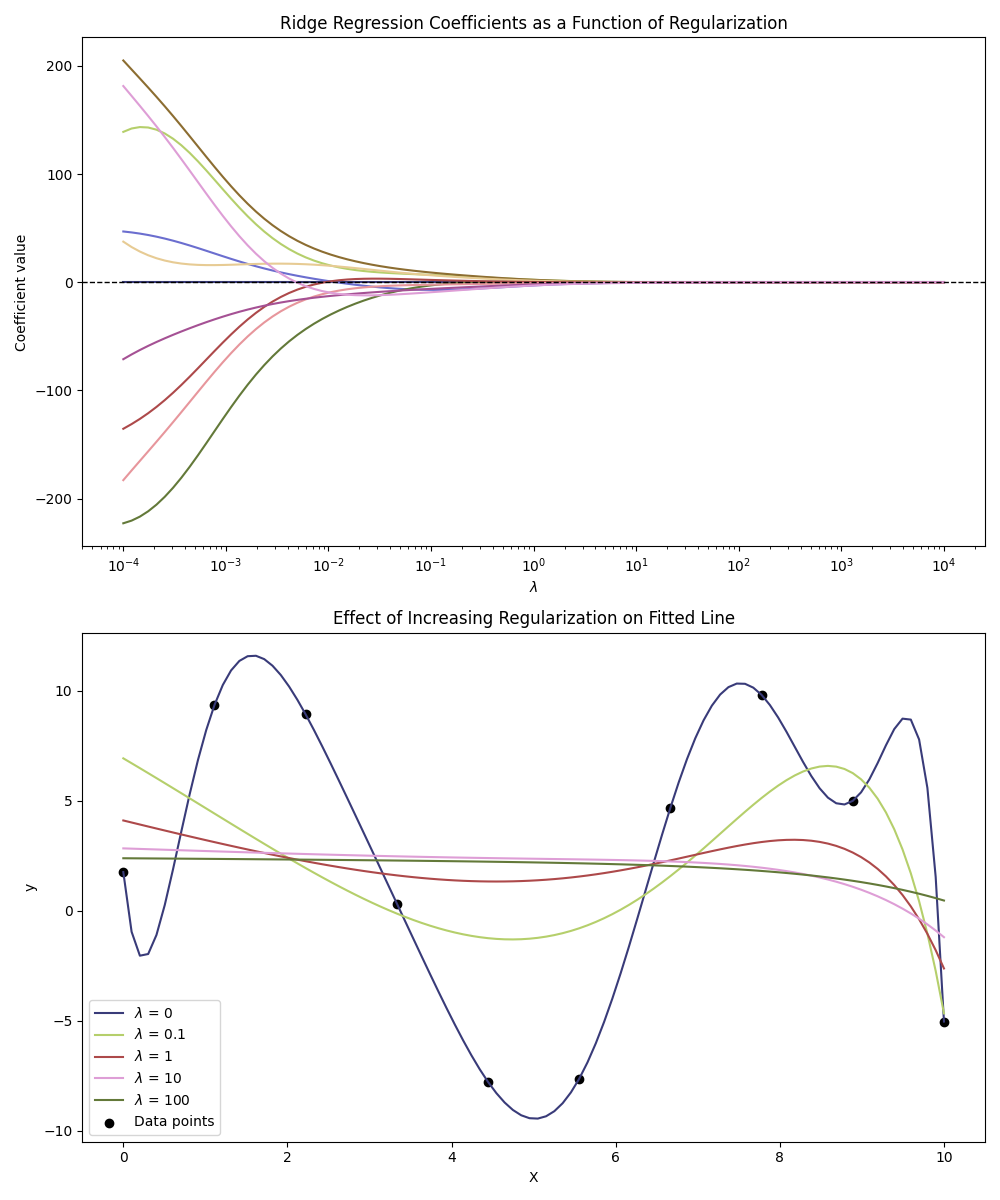
\includegraphics[width=1.0\linewidth]{img/ridge_lambda_effect}
		\caption{Ridge Regression Coefficients and the Effect of Regularization. \\ The \textbf{top plot} shows Ridge Regression coefficients as a function of the regularization parameter $\lambda$. Each line represents a different feature's coefficient, demonstrating how increasing $\lambda$ causes the coefficients to shrink towards zero. The \textbf{bottom plot} illustrates the effect of $\lambda$ on the fitted non-linear model for 10 data points (synthetic data). As $\lambda$ increases, the model transitions from overfitting (high variance) to better generalization (low variance), as seen by the smoothing of the fitted lines.}
		\label{fig:ridgelambdaeffect}
	\end{figure}
	\clearpage
	
	\begin{figure}[!t]
		\centering
		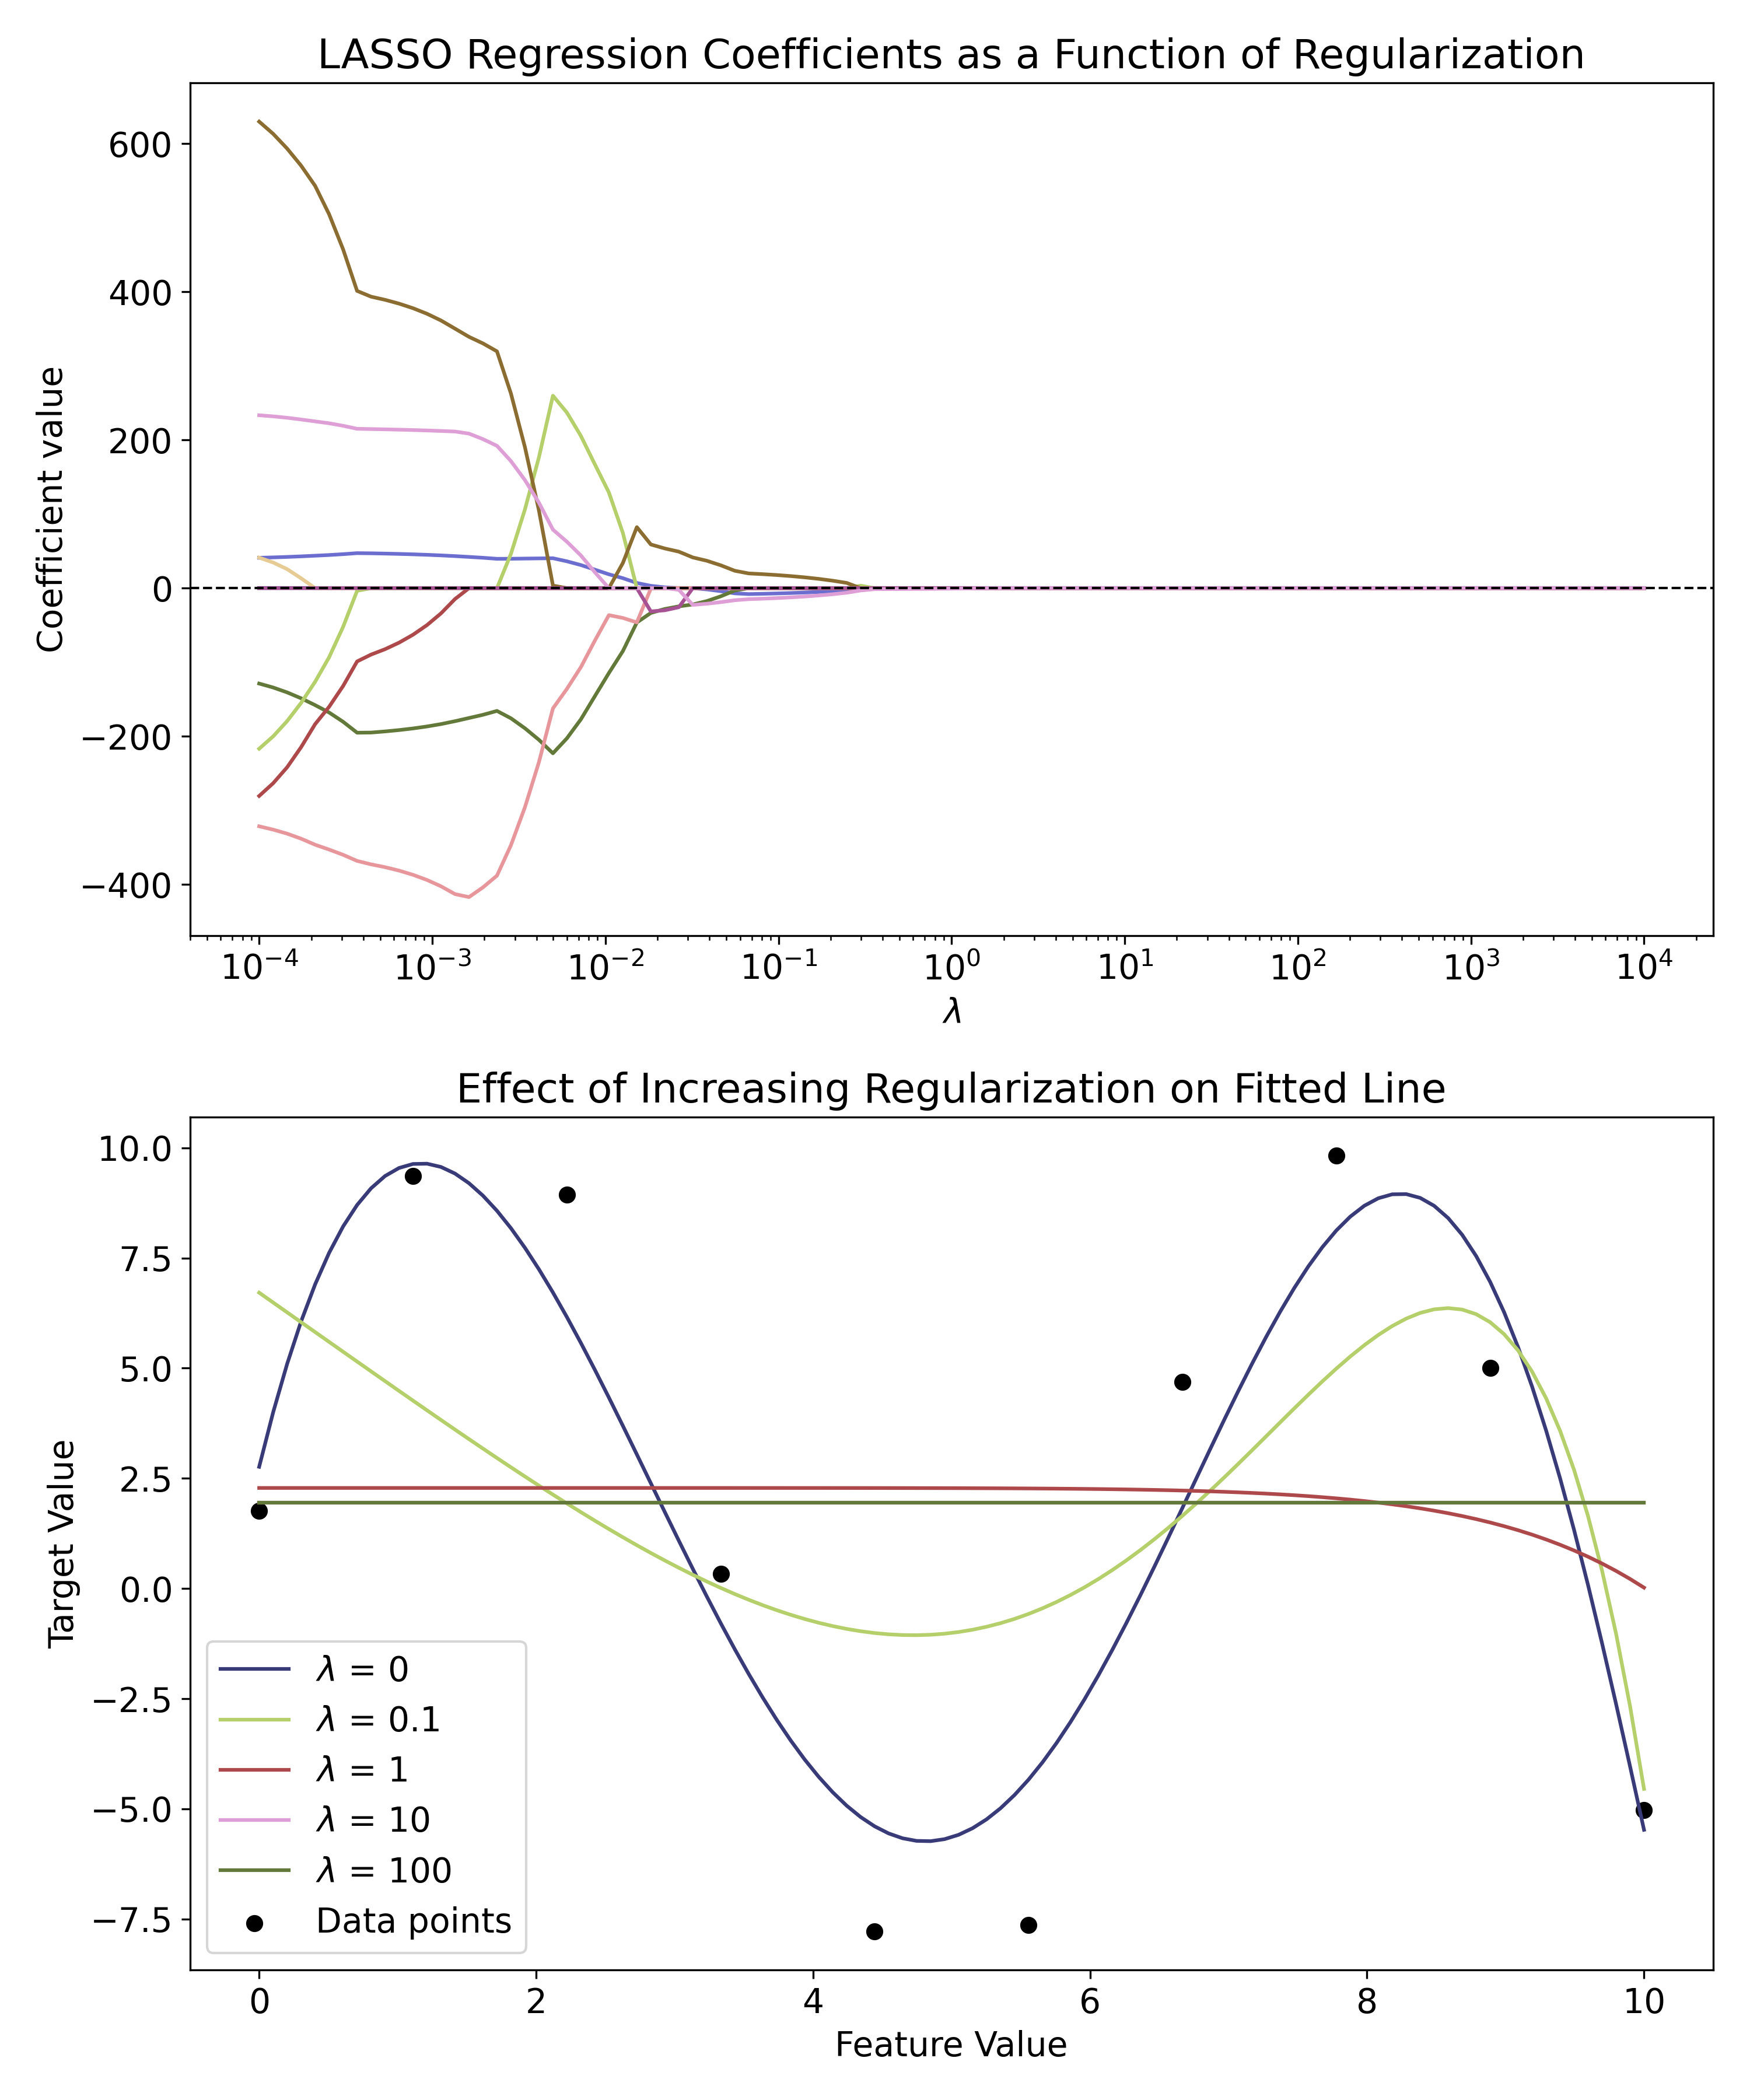
\includegraphics[width=1.0\linewidth]{img/lasso_lambda_effect}
		\caption{LASSO Regression Coefficients and the Effect of Regularization. \\ The \textbf{top plot} shows LASSO Regression coefficients as a function of the regularization parameter $\lambda$. Each line represents a different feature's coefficient, demonstrating how increasing $\lambda$ causes some coefficients to shrink to zero, effectively performing feature selection. The \textbf{bottom plot} illustrates the effect of $\lambda$ on the fitted non-linear model for 10 data points (synthetic data). As $\lambda$ increases, the model transitions from overfitting (high variance) to better generalization (low variance), as seen by the smoothing of the fitted lines.}
		\label{fig:lassolambdaeffect}
	\end{figure}
	\clearpage
	
	\subsection*{Random Forest}
	Random forest is an ensemble learning method used for both classification and regression tasks. It operates by constructing multiple decision trees during training, and outputting the mode of the classes (classification) or mean prediction (regression) of the individual trees. We will first explore how decision trees are created and move on to understanding the random forest method. Note that only the classification case will be explained, as this is the focus of the current work.
	
	\subsubsection*{Decision Trees}
	A decision tree is a flowchart-like structure in which each internal node represents a feature, each branch represents a decision rule, and each leaf node represents an outcome. The path from the root to a leaf represents classification rules \cite{hastieElementsStatisticalLearning2009}. An example of a simple decision tree is shown in Figure \ref{fig:decisiontreevisualization}A; the Gini impurity value shown in the tree will be explained in the text below.
	
	\begin{figure}[t!]
		\centering
		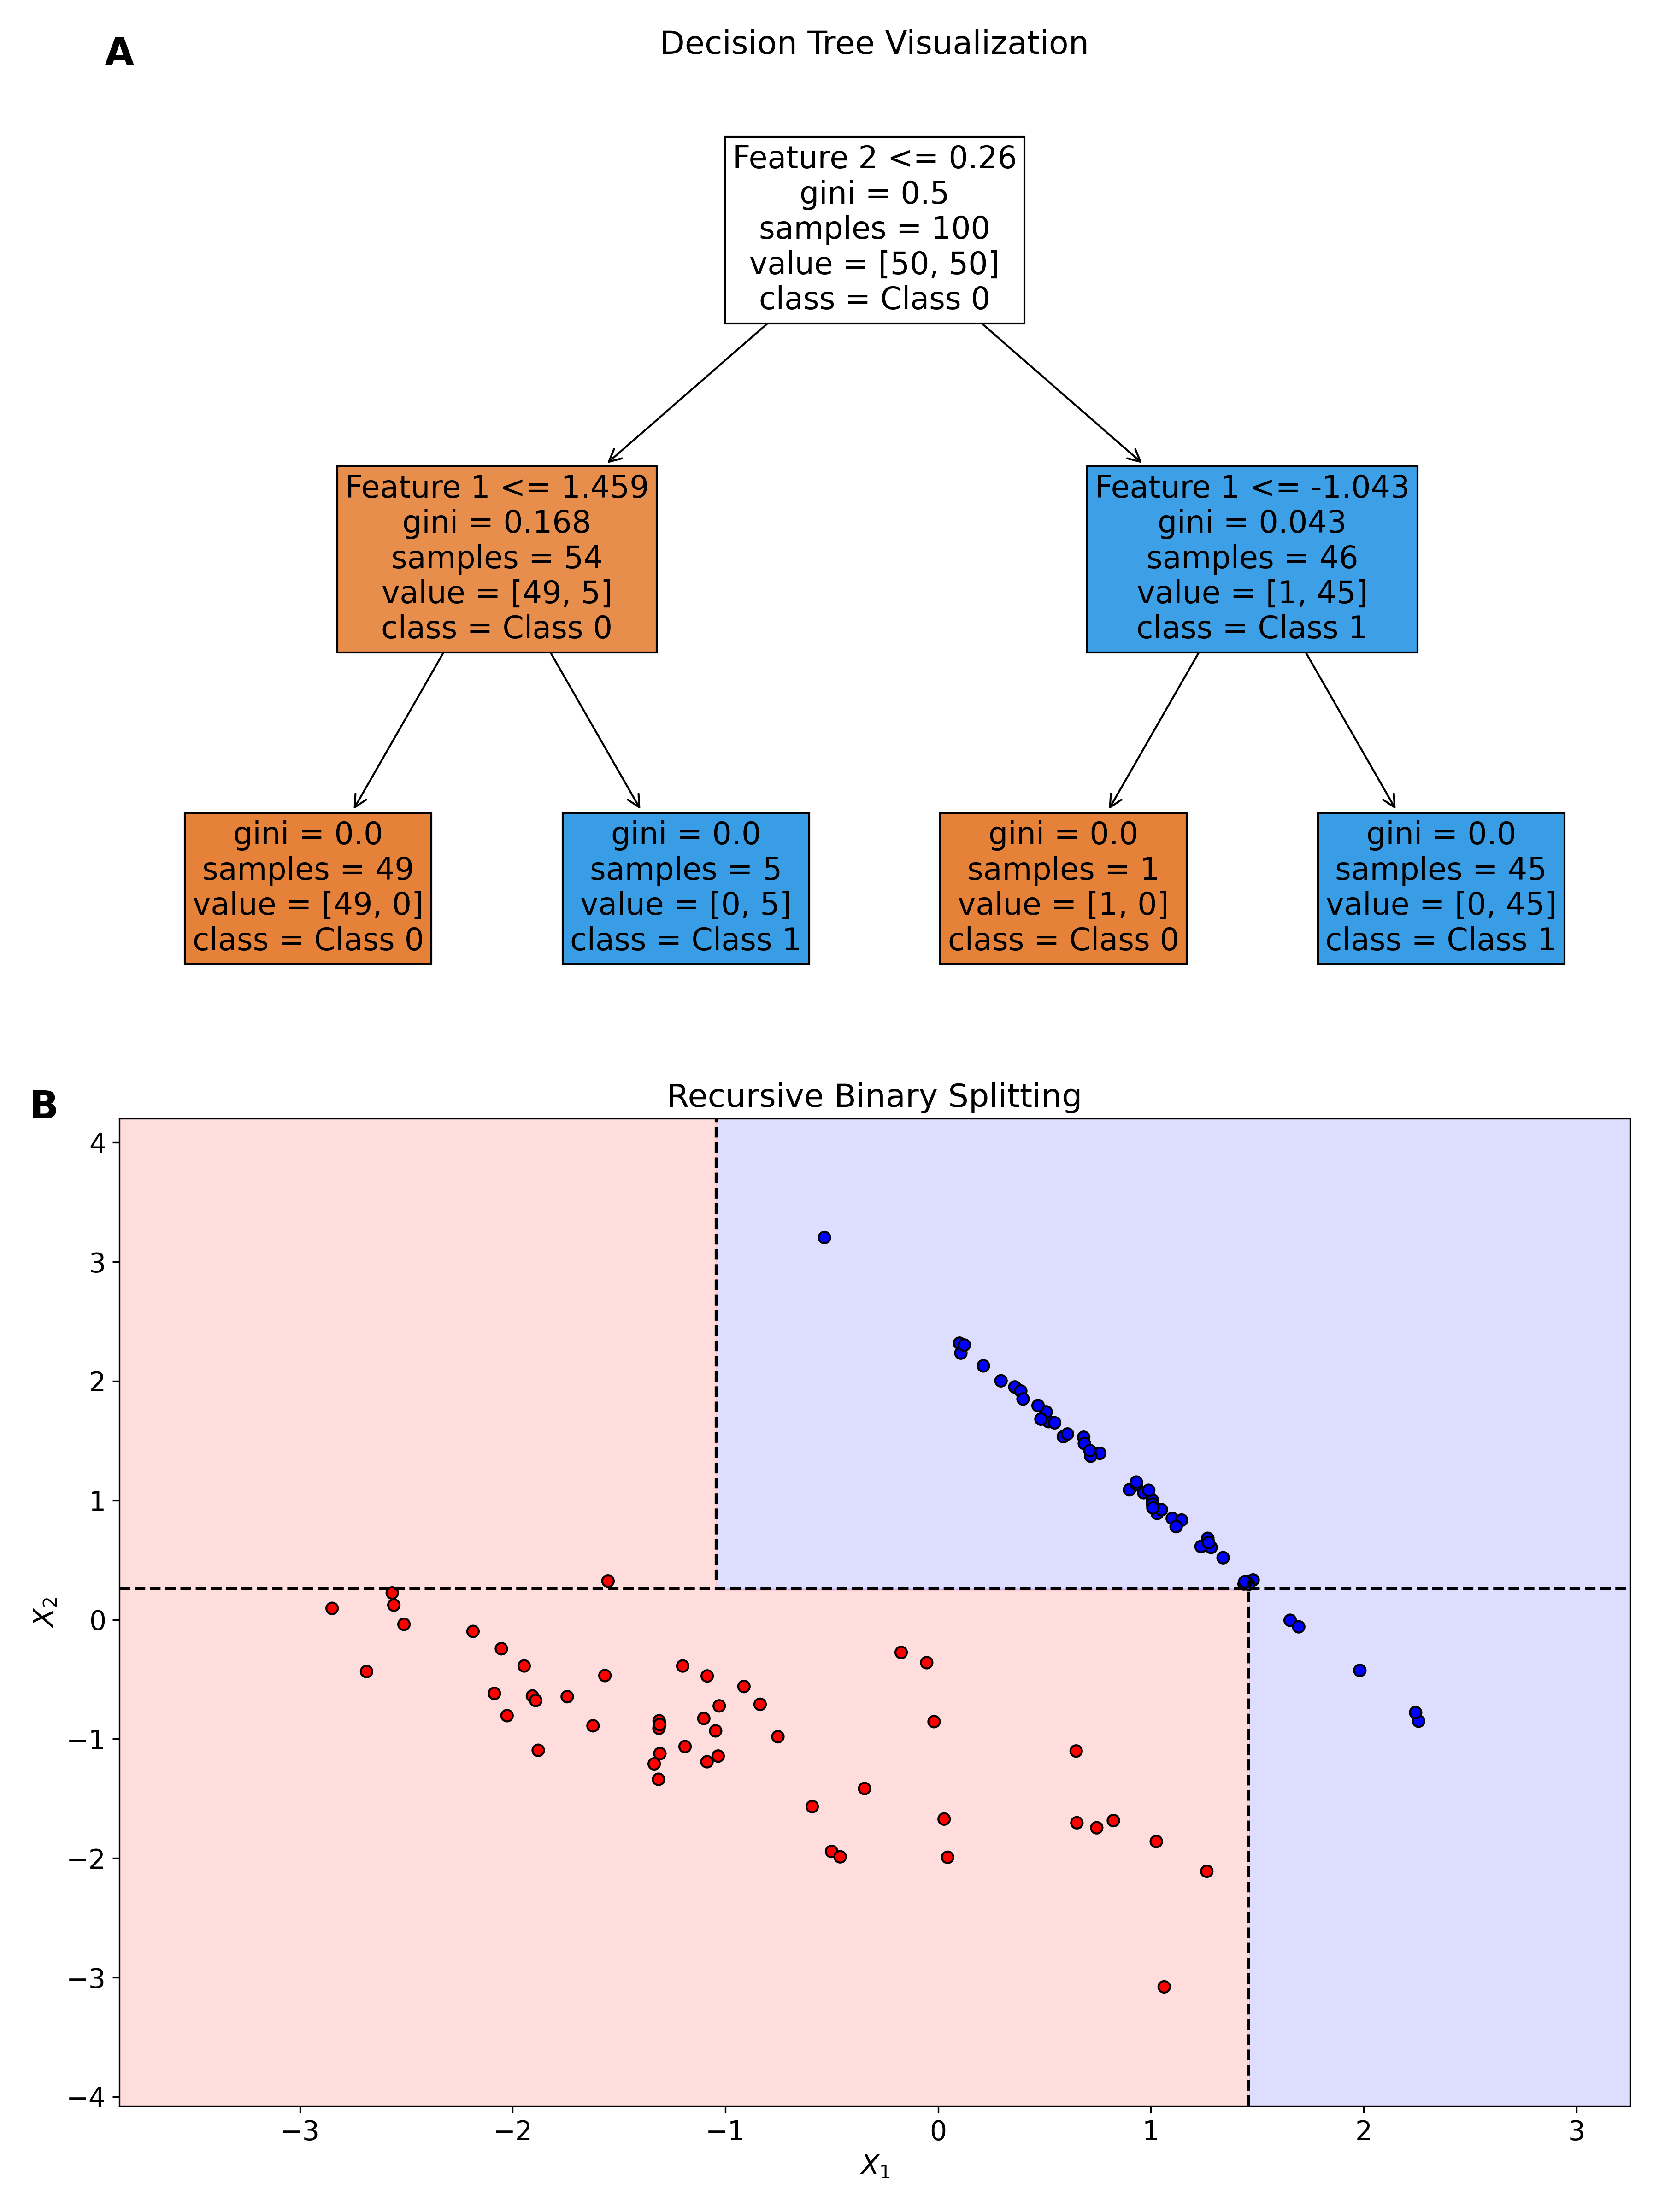
\includegraphics[width=0.9\linewidth]{img/decision_tree}
		\caption{Recursive Binary Splitting and Decision Tree Visualization. \\ This figure demonstrates the process of recursive binary splitting and the resulting decision tree on data that has two features: $X_1$ and $X_2$. The top plot (A) visualizes the decision tree, with each internal node representing a decision rule based on feature thresholds, and leaf nodes representing class outcomes. Nodes are color-coded by the majority class, with class distributions and impurity measures (Gini index) displayed. The bottom plot (B) shows the corresponding decision boundaries created by a decision tree trained on a synthetic dataset, illustrating how the feature space is recursively split into regions, as indicated by the dashed lines. }
		\label{fig:decisiontreevisualization}
	\end{figure}
	
	In constructing a decision tree, we aim to partition the feature space into regions where the response variable is as homogeneous as possible. This is done by recursively splitting the data based on certain criteria until a stopping condition is met.
	
	Given data that consists of \( p \) features and a response, for each of \( N \) observations \((x_i, y_i)\) for \( i = 1, 2, \ldots, N \), with \( x_i = (x_{i1}, x_{i2}, \ldots, x_{ip}) \), we model the response by partitioning the feature space into \( M \) regions \( R_1, R_2, \ldots, R_M \) and assigning class \( c_m \) to each region. The example in Figure \ref{fig:decisiontreevisualization} is split as follows:	
	\begin{enumerate}
		\item Feature 2 is split at \(X_2 = 0.26\) where the feature space at or below this point is assigned to class 0.
		\item Feature 1 is now split at \(X_1 = 1.459\).
		\item Finally, feature 1 is again split, now at \(X_1 = -1.043\).
	\end{enumerate}
	
	As visualized, this creates four regions in the feature space, which allows us to model the response as:
	\begin{equation*}
		\hat{f}(x) = \sum_{m=1}^{4} c_m I(x \in R_m)
	\end{equation*}
	where \( c_m \) is the class assigned to each region, and \( I(\cdots) \) is the indicator function, which is 1 if \( x \) is in region \( R_m \), and 0 otherwise. Since the data has only two classes, \( c_m \) will be either class 0 or class 1 for each region.
	
	But how do we decide where to split along each of the features? This is where we get into the splitting criterion, where there are two popular methods for classification tasks:
	
	\begin{itemize}
		\item \textbf{Gini impurity}:
		\begin{equation*}
			G = \sum_{i=1}^{C}p_i(1-p_i)
		\end{equation*}
		where $p_i$ is the probability of class $i$ in the node. This measures how often a randomly chosen element would be incorrectly classified.
		\item \textbf{Entropy}:
		\begin{equation*}
			H = -\sum_{i=1}^{C}p_i\log(p_i)
		\end{equation*}
		This measures the disorder or randomness of the data points in the node.
	\end{itemize}
	Since it is preferable to minimize both the Gini impurity and the entropy, the following step works for either criterion. Consider a feature \( j \) and a split point \( s \), and define the regions:
	\begin{equation*}
		R_1(j, s) = \{X|X_j \leq s\}\ \text{and}\ R_2(j, s) = \{X|X_j > s\}
	\end{equation*}
	
	The goal is then to find a \( j \) and \( s \) that minimize the function:
	\begin{equation*}
		\min_{j,s} \left[\frac{N_{R_1}}{N}C_{R_1} + \frac{N_{R_2}}{N}C_{R_2}\right]
	\end{equation*}
	where \( N_{R_1} \) and \( N_{R_2} \) are the number of samples in \( R_1 \) and \( R_2 \), and \( C_{R_1} \) and \( C_{R_2} \) is the splitting criterion value of these regions.
	
	After finding the best split, we now assign the class label for each region \( R_m \) as the majority class in that region:
	\begin{equation*}
		c_m = \arg \max_k \sum_{x_i \in R_m} I(y_i = k)
	\end{equation*}
	that is, the class label assigned for a given region is the class that appears most frequently within that region \cite{hastieElementsStatisticalLearning2009,sohilIntroductionStatisticalLearning2022}.
	
	Utilizing the functions mentioned so far for producing a decision tree could, however, lead to a problematic situation. One way to optimize the tree would be to grow it deep enough to assign each data point to its own node, resulting in an overly complex model. To prevent this, several methods can be employed:
	\begin{itemize}
		\item \textbf{Maximum depth}: Directly limit how deep the tree is allowed to grow.
		\item \textbf{Minimum samples per leaf}: Require a minimum number of samples in each leaf to avoid splits that result in nodes with very few data points.
		\item \textbf{Minimum samples per split}: Require a minimum number of samples to be present at a node before it can be split further.
		\item \textbf{Maximum leaf nodes}: Limit the number of leaf nodes in the tree to prevent excessive growth.
	\end{itemize}
	
	Once again, determining the optimal value for these hyperparameters is typically done through cross-validation.
	
	\subsubsection*{Random Forest}
	Building on the foundation of decision trees, random forest enhances the model's performance by combining multiple decision trees to form an ensemble. Each tree in the random forest is built using a bootstrap sample of the data, and at each split, a random subset of features is considered for splitting. The randomness helps in creating diverse trees that reduce the overall variance of the model.
	
	The random forest algorithm involves the following steps:
	\begin{enumerate}
		\item \textbf{Bootstrap sampling}: Randomly sample the dataset with replacement to create multiple bootstrap samples. Each tree is trained on a different bootstrap sample, introducing variability in the training data.
		\item \textbf{Tree construction}: For each bootstrap sample, grow a decision tree using a random subset of features at each split. This random selection of features further decorrelates the trees.
		\item \textbf{Aggregation}: Aggregate the predictions of all the trees to make the final prediction. For classification, the mode of the predicted classes is used.
	\end{enumerate}
	
	One might notice the aggressive attempt at decorrelating different trees in random forests. The reason for this is that if we can successfully create an ensemble of decorrelated trees, the variance of the model is reduced significantly more than if the trees are correlated. To understand this, consider \( n \) uncorrelated random variables \( X_1, X_2, \ldots, X_n \), each with the same variance \( \sigma^2 \). The variance of the sum of these variables is the sum of their variances \cite{moodIntroductionTheoryStatistics1973}. Mathematically:
	\begin{equation*}
		\text{Var}\left(\frac{1}{n} \sum_{i=1}^{n} X_i \right) = \frac{1}{n^2} \sum_{i=1}^{n} \text{Var}(X_i)
	\end{equation*}
	Simplifying:
	\begin{equation*}
		\frac{1}{n^2} \sum_{i=1}^{n} \text{Var}(X_i) = \frac{1}{n^2} \sum_{i=1}^{n} \sigma^2 = \frac{\sigma^2}{n}
	\end{equation*}
	Thus, the variance of the average of uncorrelated random variables decreases proportionally to \( \frac{1}{n} \).
	
	Now, if we instead consider \( n \) random variables \( X_1, X_2, \ldots, X_n \) that are highly correlated, let \( \rho \) represent the average correlation coefficient between any two variables.  For correlated variables, the covariance \( \text{Cov}(X_i, X_j) \) for \( i \neq j \) is \( \rho \sigma^2 \). 
	
	The variance now includes both the variance of the individual variables and the covariance between them:
	\begin{equation*}
		\text{Var}\left(\frac{1}{n}\sum_{i=1}^{n}X_i\right) = \frac{1}{n^2} \left(\sum_{i=1}^{n} \text{Var}(X_i) + \sum_{i \neq j} \text{Cov}(X_i, X_j)\right)
	\end{equation*}
	Given that \( \text{Var}(X_i) = \sigma^2 \) and \( \text{Cov}(X_i, X_j) = \rho \sigma^2 \), we can simplify further:
	\begin{align*}
		\frac{1}{n^2} \left(\sum_{i=1}^{n} \text{Var}(X_i) + \sum_{i \neq j} \text{Cov}(X_i, X_j)\right) &= \frac{1}{n^2}(n\sigma^2 + n(n-1)\rho\sigma^2) \\
		&= \frac{\sigma^2}{n} + \rho\sigma^2\left(1 - \frac{1}{n}\right)
	\end{align*}
	
	This shows that the variance reduction achieved through averaging is much less significant when the variables are correlated, as the additional term \( \rho\sigma^2\left(1 - \frac{1}{n}\right) \) does not decrease as rapidly with increasing \( n \). Hence, the effectiveness of random forests in reducing variance is due to the decorrelation of trees, leading to a more robust and generalizable model.
	
	\subsection*{Support Vector Machines (SVMs)}
	Support Vector Machines (SVMs) are a powerful set of supervised learning methods used for classification, regression, and outlier detection. They are particularly effective in high-dimensional spaces and are versatile in terms of the different kernel functions that can be specified for the decision function.
	
	\subsubsection*{Mathematical Formulation}
	The primary goal of SVM is to find a hyperplane in an \( N \)-dimensional space (\( N \) being the number of features) that distinctly classifies the data points. The best hyperplane for an SVM means the one with the largest margin between the classes.
	
	\begin{equation*}
		\text{maximize} \quad M = \frac{2}{||\mathbf{w}||}
	\end{equation*}
	
	Subject to the constraints:
	\begin{equation*}
		y_i (\mathbf{w} \cdot \mathbf{x}_i + b) \geq 1 \quad \text{for all } i
	\end{equation*}
	
	Here, \( \mathbf{w} \) is the weight vector, \( \mathbf{x}_i \) are the feature vectors, \( y_i \) are the class labels, and \( b \) is the bias term. The margin \( M \) is defined as the distance between the hyperplane and the nearest data point from either class \cite{hastieElementsStatisticalLearning2009,cortesSupportvectorNetworks1995}. 
	
	\subsubsection*{Soft Margin SVM}
	In many real-world scenarios, data may not be perfectly linearly separable. To handle such cases, SVMs introduce slack variables \( \xi_i \) to allow some misclassifications:
	
	\begin{equation*}
		\text{minimize} \quad \frac{1}{2} ||\mathbf{w}||^2 + C \sum_{i=1}^{n} \xi_i
	\end{equation*}
	
	Subject to:
	\begin{equation*}
		y_i (\mathbf{w} \cdot \mathbf{x}_i + b) \geq 1 - \xi_i \quad \text{and} \quad \xi_i \geq 0 \quad \text{for all } i
	\end{equation*}
	
	Here, \( C \) is a regularization parameter that controls the trade-off between maximizing the margin and minimizing the classification error \cite{hastieElementsStatisticalLearning2009,sohilIntroductionStatisticalLearning2022}.
	
	\subsubsection*{Kernel Trick}
	The power of SVMs lies in their ability to use kernel functions to handle non-linearly separable data by mapping the input features into high-dimensional feature spaces. Commonly used kernels include:
	
	\begin{itemize}
		\item \textbf{Linear kernel}: \( K(\mathbf{x}_i, \mathbf{x}_j) = \mathbf{x}_i \cdot \mathbf{x}_j \)
		\item \textbf{Polynomial kernel}: \( K(\mathbf{x}_i, \mathbf{x}_j) = (\mathbf{x}_i \cdot \mathbf{x}_j + 1)^d \)
		\item \textbf{Radial Basis Function (RBF) kernel}: \( K(\mathbf{x}_i, \mathbf{x}_j) = \exp(-\gamma ||\mathbf{x}_i - \mathbf{x}_j||^2) \)
		\item \textbf{Sigmoid kernel}: \( K(\mathbf{x}_i, \mathbf{x}_j) = \tanh(\alpha \mathbf{x}_i \cdot \mathbf{x}_j + c) \)
	\end{itemize}
	
	The kernel trick allows SVMs to perform linear separation in these higher-dimensional spaces without explicitly computing the coordinates of the data in that space \cite{sohilIntroductionStatisticalLearning2022,hastieElementsStatisticalLearning2009} (see Figure \ref{fig:svm_examples}).
	
	\subsubsection*{Properties and Benefits}
	\begin{itemize}
		\item \textbf{Effective in high-dimensional spaces}: SVMs are particularly effective when the number of dimensions exceeds the number of samples.
		\item \textbf{Memory efficiency}: Only a subset of training points (support vectors) are used in the decision function.
		\item \textbf{Versatility}: Different kernel functions can be specified for the decision function, making SVMs a versatile tool for various types of data.
	\end{itemize}
	
	\begin{figure}[th]
		\centering
		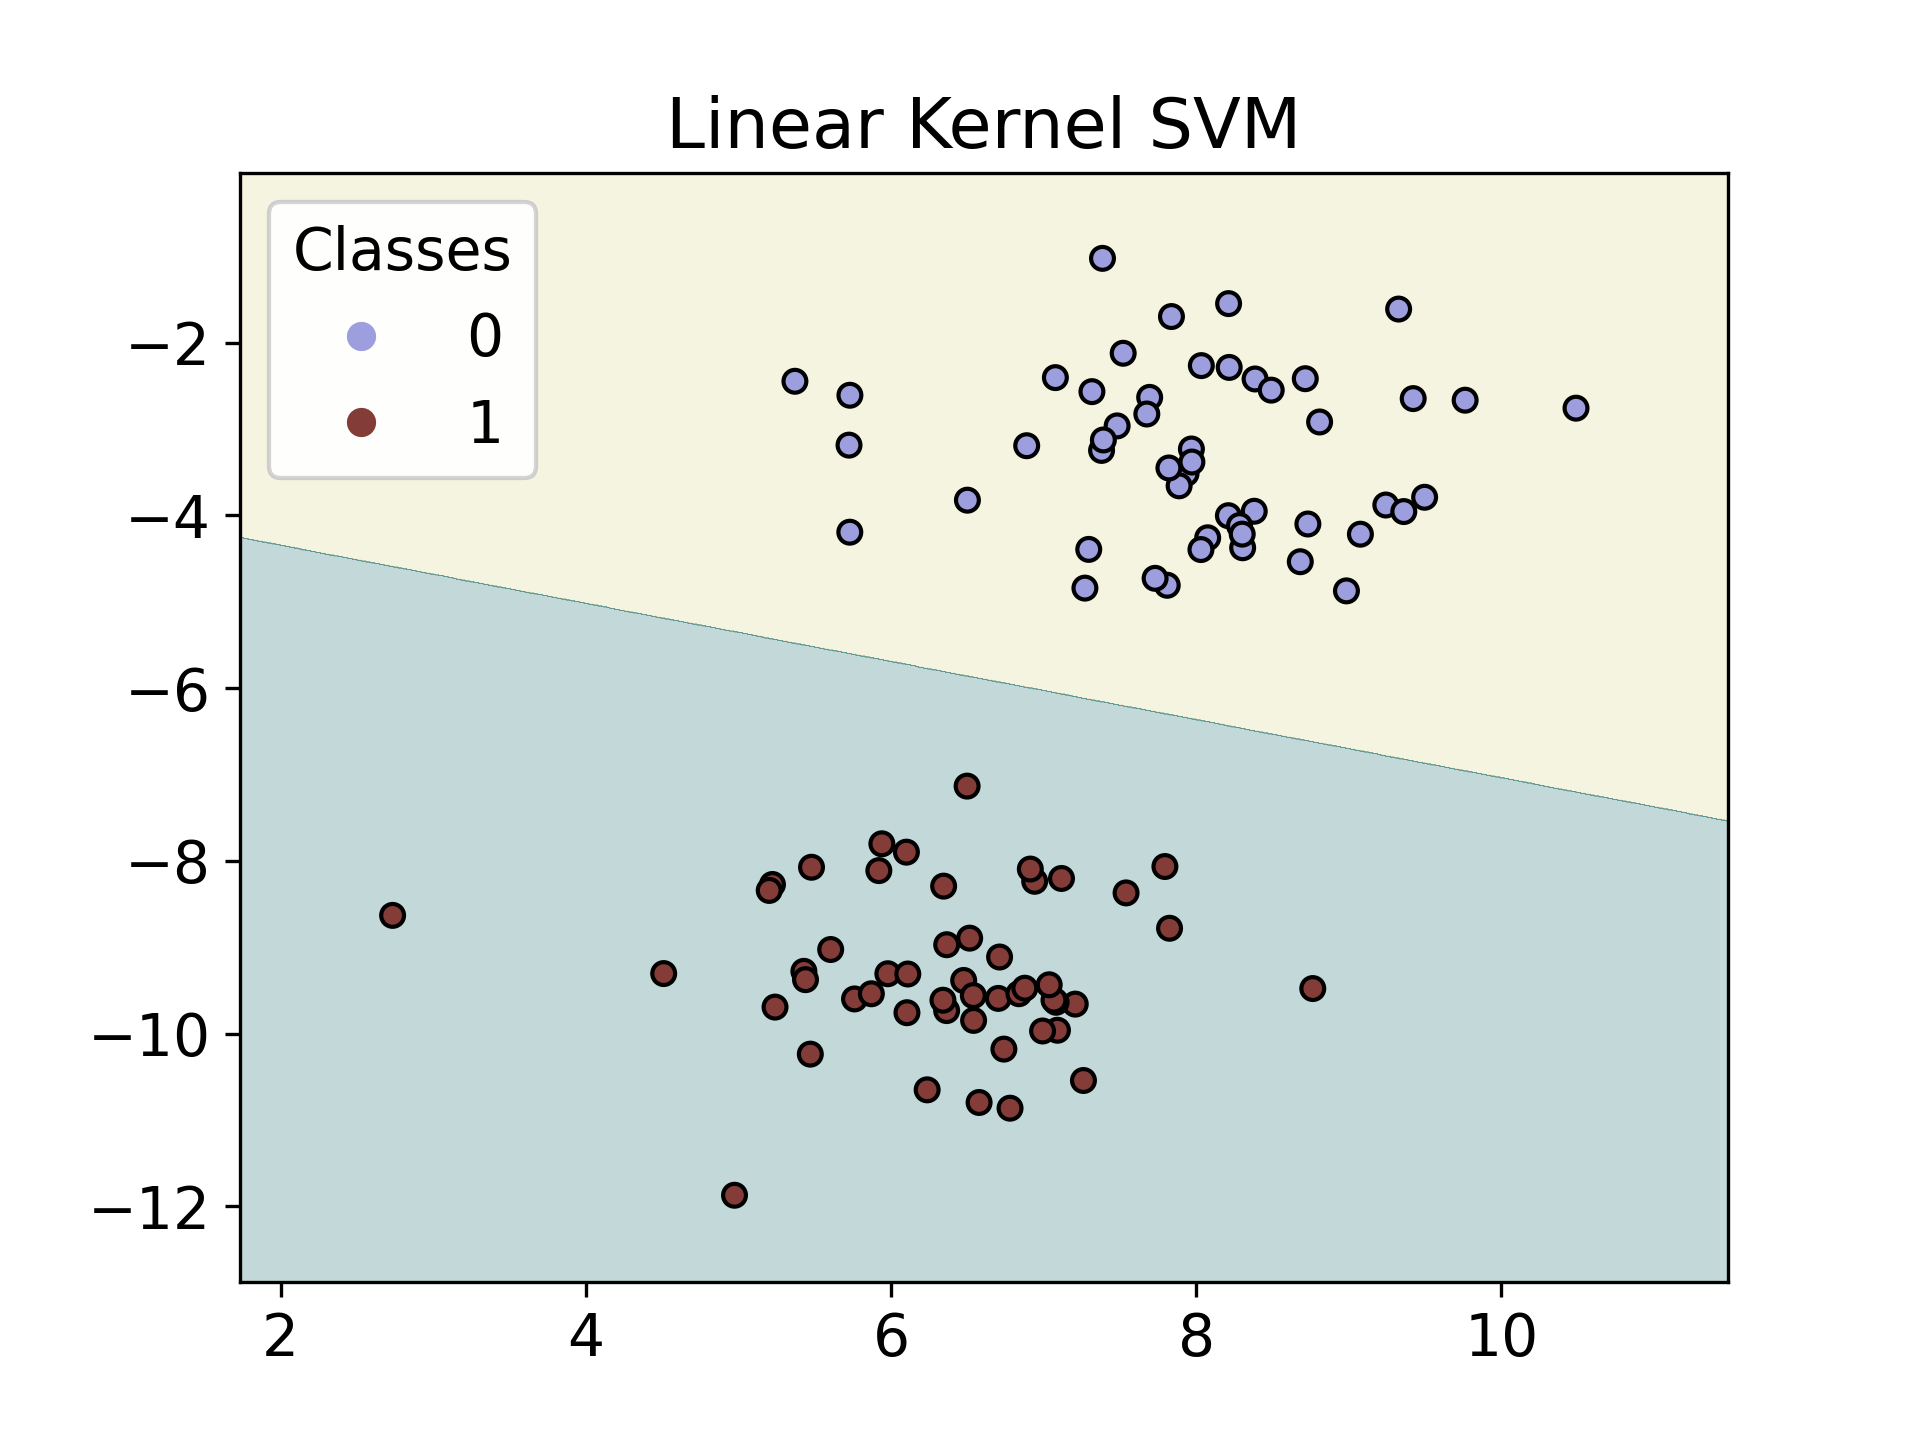
\includegraphics[width=0.45\linewidth]{img/svm_linear.png}
		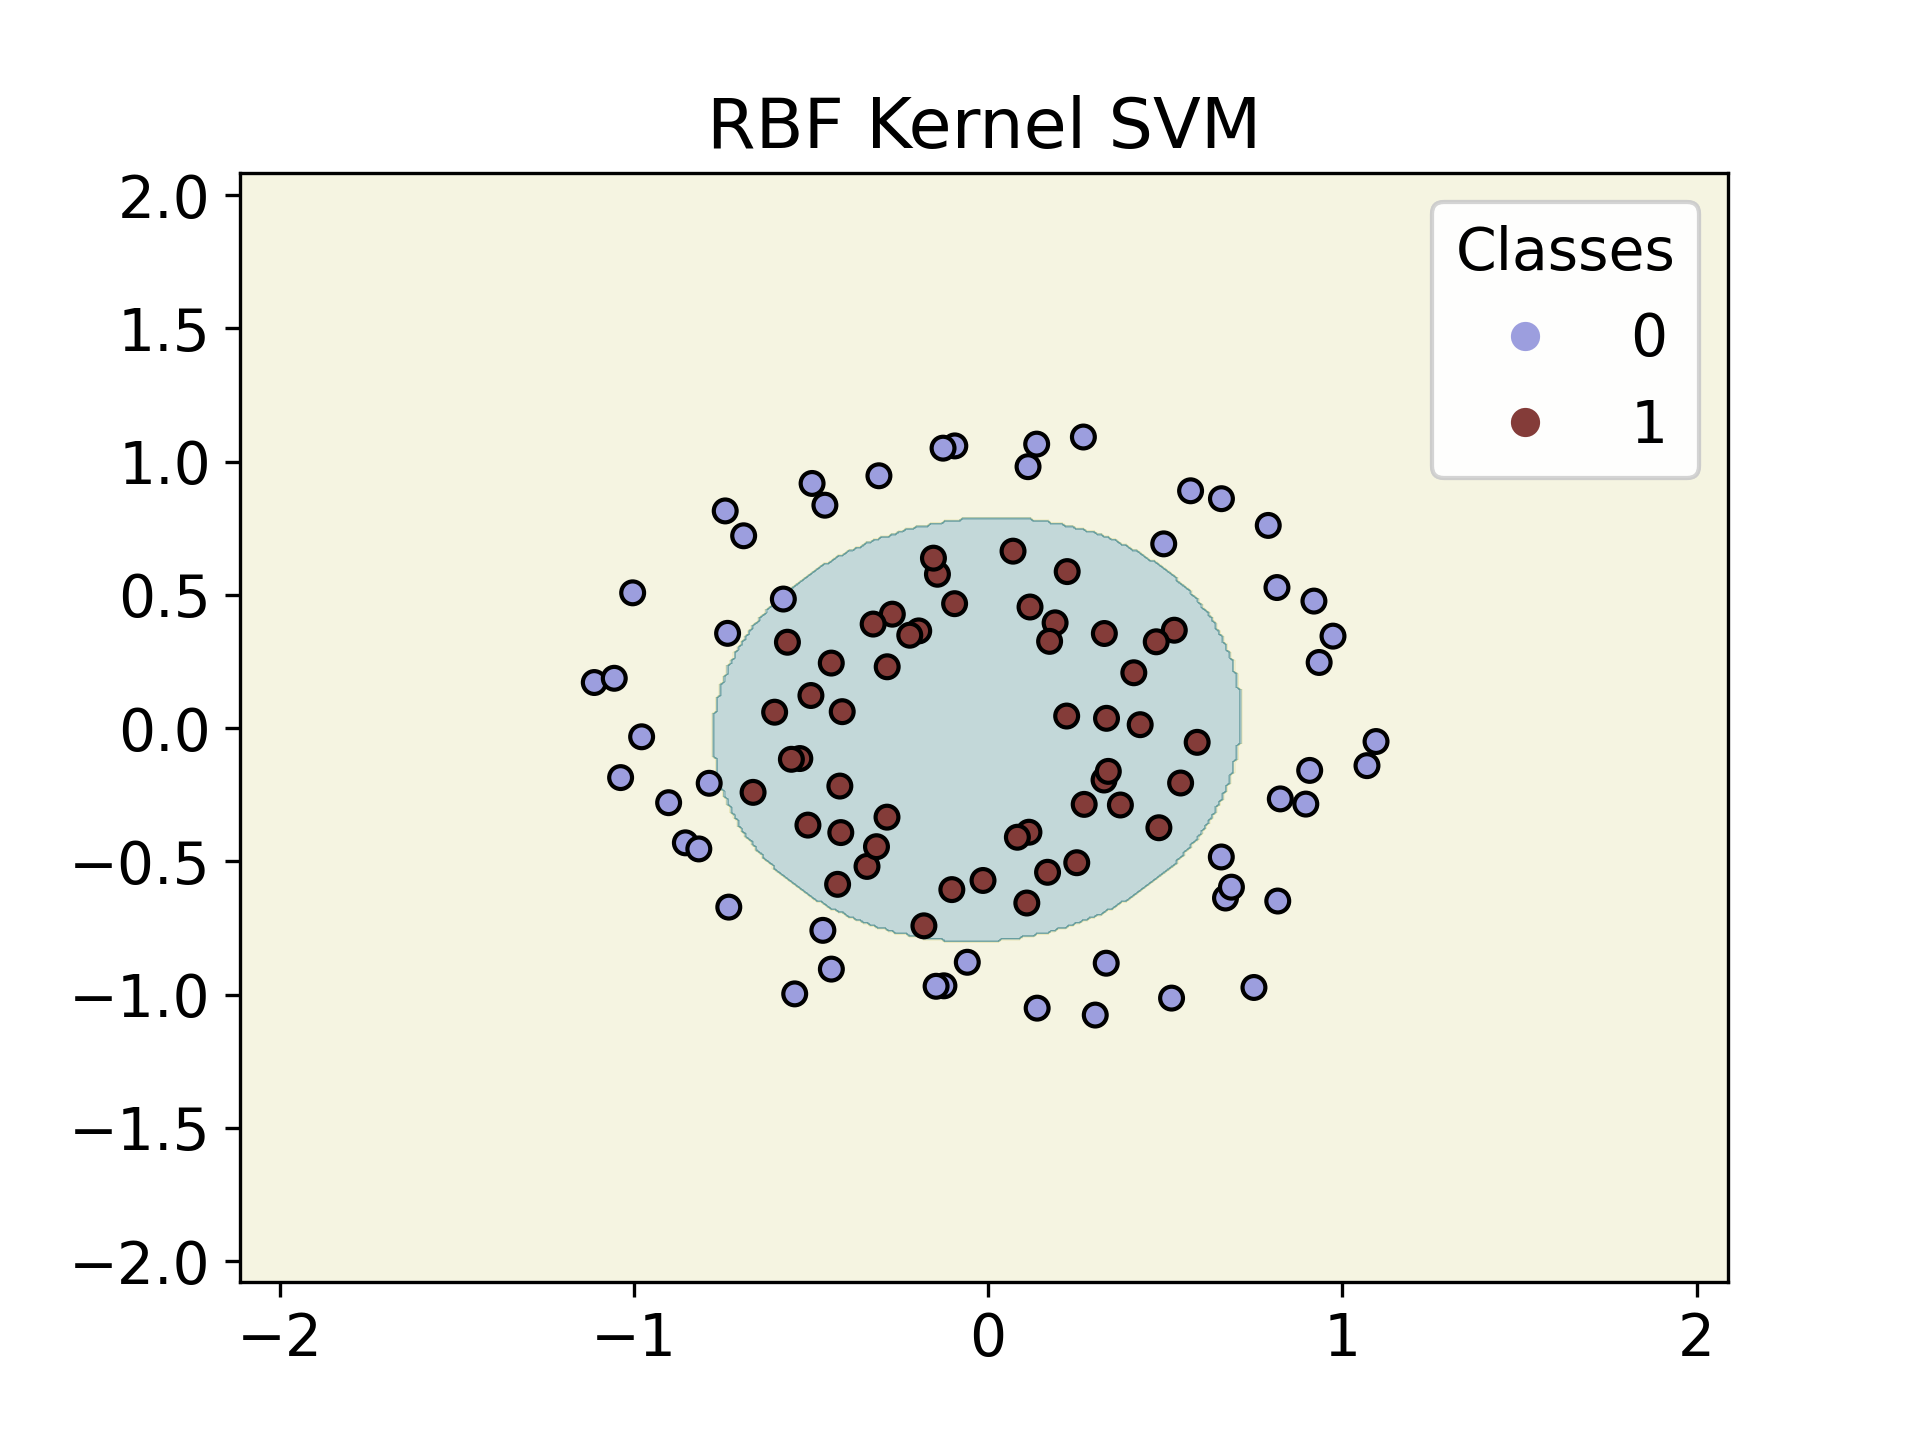
\includegraphics[width=0.45\linewidth]{img/svm_nonlinear.png}
		\caption{Support Vector Machines: Linear and Non-linear Decision Boundaries. \\ \textbf{Left}: SVM with a linear kernel creating a linear decision boundary. \textbf{Right}: SVM with a radial basis function (RBF) kernel creating a non-linear decision boundary.}
		\label{fig:svm_examples}
	\end{figure}
	
	\subsubsection*{Hyperparameter Tuning}
	Choosing the right hyperparameters, such as the regularization parameter \( C \) and kernel-specific parameters like \( \gamma \) for the RBF kernel, is crucial for the performance of SVMs. Techniques such as cross-validation can be used to tune these parameters.
	
	In conclusion, SVMs provide a robust method for classification tasks, especially in high-dimensional spaces. Their ability to handle non-linearly separable data through kernel functions make them highly versatile and effective in diverse applications.
	
	\subsection*{Neural Networks}
	Neural networks are a class of machine learning models inspired by the human brain's structure and function. They consist of layers of interconnected neurons (nodes), each performing a simple computation. Neural networks are capable of learning complex patterns in data and have been successfully applied to a wide range of tasks, including image recognition, natural language processing, robotics, finance, and more.
	
	\subsubsection*{Perceptron Algorithm}
	The perceptron algorithm, developed by Frank Rosenblatt in 1957 \cite{rosenblattPerceptronProbabilisticModel1958}, is a fundamental building block of neural networks. It is a type of linear classifier, used for binary classification tasks. The perceptron algorithm updates its weights iteratively to minimize classification errors.

	The Perceptron algorithm works as follows:
	\begin{enumerate}
		\item Initialize the weights to small random values.
		\item For each training example, compute the output:
		\begin{equation*}
			\hat{y} = \begin{cases}
				1 & \text{if } \mathbf{w} \cdot \mathbf{x} + b > 0 \\
				0 & \text{otherwise}
			\end{cases}
		\end{equation*}
		\item Update the weights if there is a misclassification:
		\begin{equation*}
			\mathbf{w} \leftarrow \mathbf{w} + \eta (y - \hat{y}) \mathbf{x}
		\end{equation*}
		\item Repeat steps 2 and 3 until convergence or for a fixed number of iterations.
	\end{enumerate}
	
	Here, \( \mathbf{w} \) represents the weight vector, \( \mathbf{x} \) is the input vector, \( b \) is the bias, \( y \) is the true label, \( \hat{y} \) is the predicted label, and \( \eta \) is the learning rate. Figure \ref{fig:perceptron_algorithm} shows a visualization of this process.
	
	\begin{figure}[h]
		\centering
		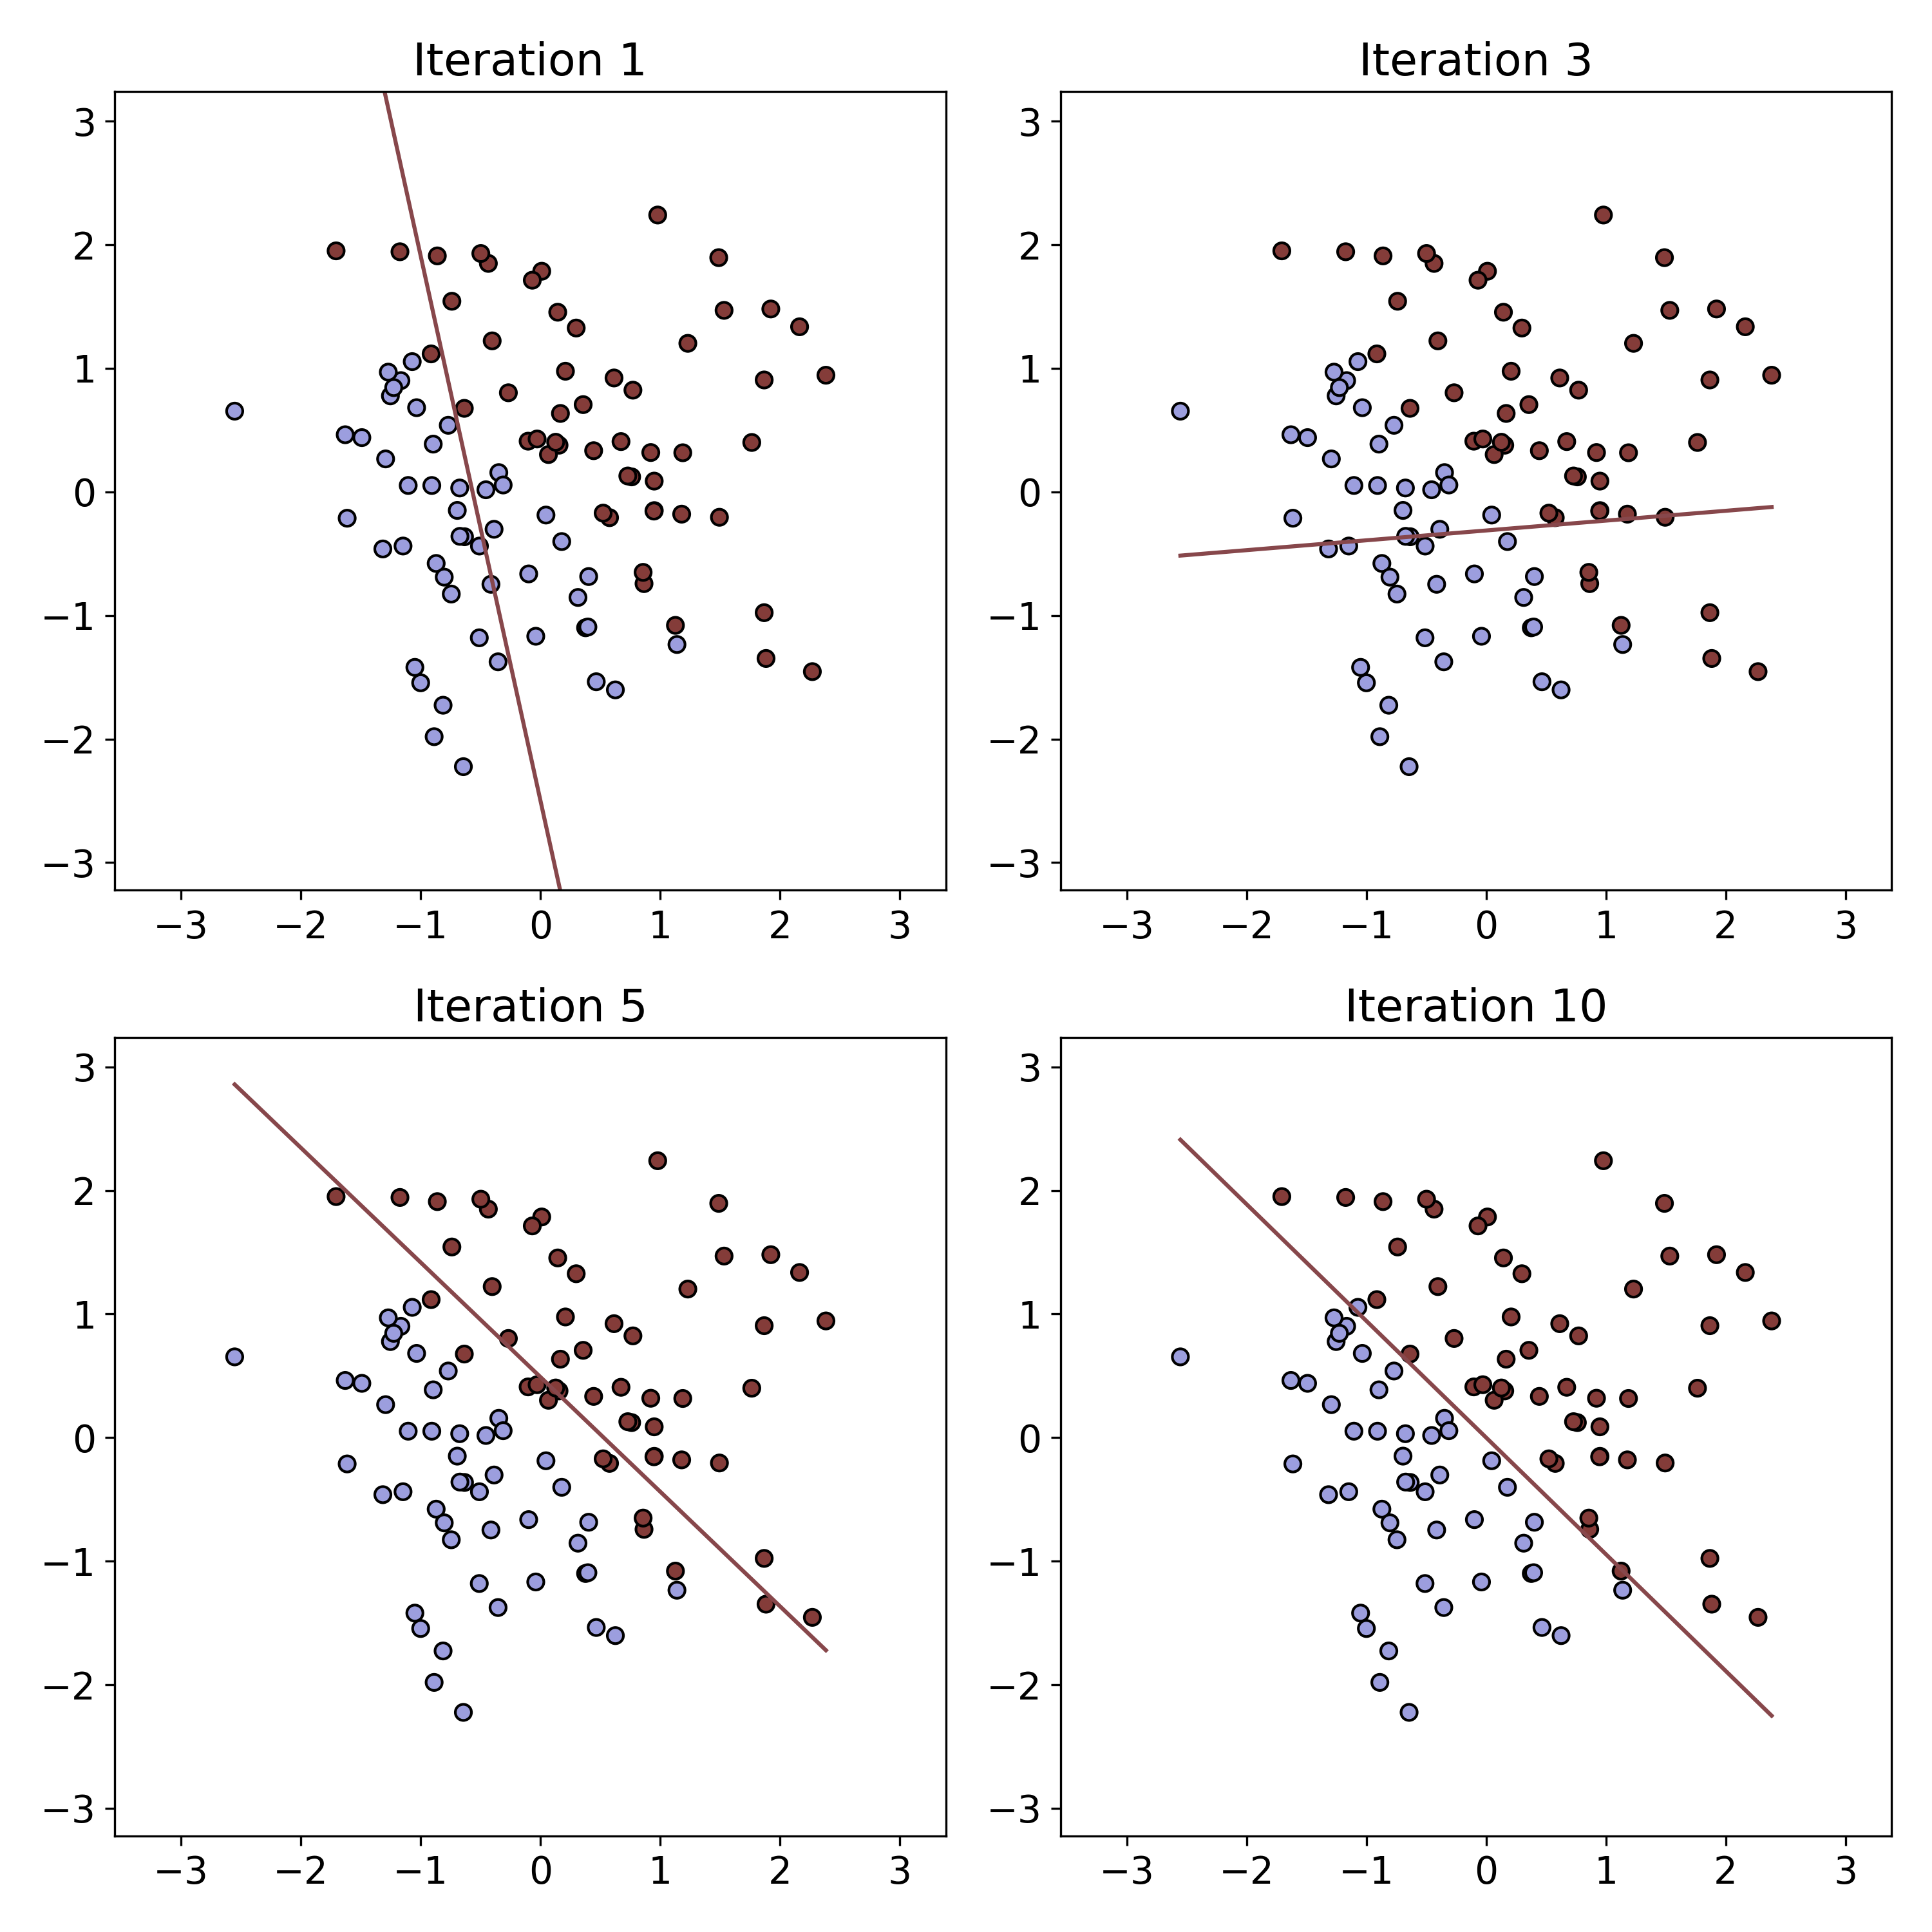
\includegraphics[width=0.8\linewidth]{img/perceptron.png}
		\caption{Perceptron algorithm process. The figure shows the progression of the decision boundary (solid line) over multiple iterations of the algorithm.}
		\label{fig:perceptron_algorithm}
	\end{figure}
	
	\subsubsection*{Multi-Layer Perceptron}
	The Multi-Layer Perceptron (MLP) is an extension of the perceptron, consisting of multiple layers of neurons, including input, hidden, and output layers. Each layer in an MLP performs a linear transformation followed by a non-linear activation function, enabling the network to learn complex, non-linear patterns \cite{hintonConnectionistLearningProcedures1989}. Figure \ref{fig:perceptron_vs_mlp} shows a comparison between the perceptron and MLP on a non-linearly separable dataset.
	
	\begin{figure}[h]
		\centering
		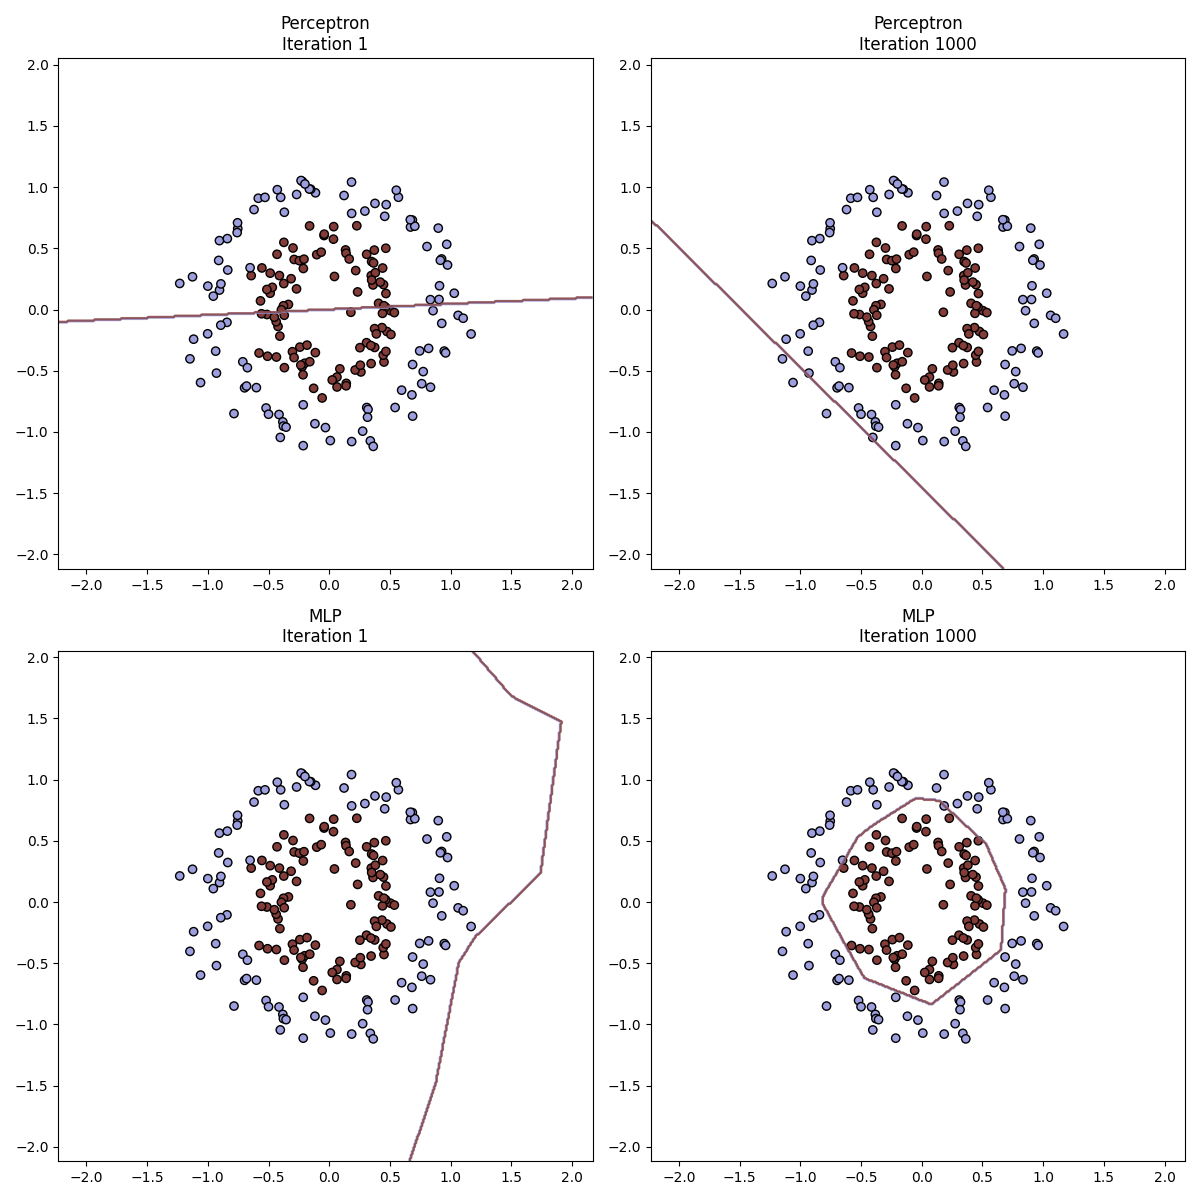
\includegraphics[width=0.8\linewidth]{img/perceptron_vs_mlp.png}
		\caption{Comparison of perceptron and Multi-Layer Perceptron (MLP) on a non-linearly separable dataset. The top plots show the decision boundary progression for a Perceptron, while the bottom plots show the progression for an MLP.}
		\label{fig:perceptron_vs_mlp}
	\end{figure}
	
	\subsubsection*{Universal Approximation Theorem}
	The universal approximation theorem states that a feed-forward neural network with a single hidden layer containing a finite number of neurons can approximate any continuous function on compact subsets of \(\mathbb{R}^n\), given sufficient number of neurons in the hidden layer \cite{hornikMultilayerFeedforwardNetworks1989}. This theorem deserves some attention to understand what it says, so let us break down the key parts:
	\begin{itemize}
		\item \textbf{Feed-forward neural network}: Neural network that takes some input data, passes it through its layers, and generates an output. The feed-forward process will be explained in further details below.
		\item \textbf{Compact subsets of \( \mathbb{R}^n \) }: This means that we are looking at functions defined in a specific, limited region of space (imagine a box in the \(n\)-dimensional space). The term "compact" ensures that this region is finite and closed, meaning it includes its boundary.
	\end{itemize}
	To reiterate, the theorem tells us that with just one hidden layer and a sufficient number of neurons, a neural network can model highly complex behaviors and patterns in data. This underscores the theoretical power of neural networks to approximate any continuous function effectively:
	\begin{equation*}
		f(x) = \sum_{i=1}^{N} \alpha_i \sigma(\mathbf{w}_i \cdot \mathbf{x} + b_i)
	\end{equation*}
	where \( \sigma \) is an activation function, \( \mathbf{w}_i \) are the weights, \( \alpha_i \) and \( b_i \) are coefficients and biases \cite{hornikMultilayerFeedforwardNetworks1989}.
	
	\subsubsection*{Feed-Forward Process}
	The feed-forward process in a neural network involves taking the input data and passing it through each layer of the network to produce an output. Think of it as a flow of information from the input layer, through any hidden layers, and finally to the output layer. Each neuron in these layers takes the inputs it receives, processes them by applying certain weights (which can be thought of as importance levels), adds a bias (an additional adjustable value), and then passes this result through an activation function (which decides whether the neuron should be activated or not, much like a gate that either opens or closes).
	
	\textbf{Example:}
	Imagine a neural network designed to recognize handwritten digits. The input layer receives an image of a digit. This image is passed through a hidden layer of neurons, each of which transforms the input in some way and sends it to the next layer. Finally, the output layer produces the network's prediction of what digit the image represents.
	
	\subsubsection*{Backpropagation Algorithm}
	Backpropagation is a method used to train neural networks by adjusting the weights and biases to minimize the error in the network's predictions. After the feed-forward process, the network's output is compared to the actual target output, and the difference (or error) is calculated using a loss function. The loss function quantifies how well the network's predictions match the actual targets, guiding the optimization process. Backpropagation then works backward through the network to update the weights and biases so that the next time the same input is presented, the network's prediction will be closer to the actual target.
	
	This process involves two main steps:
	\begin{enumerate}
		\item \textbf{Forward Pass:} Just like in the feed-forward process, the input data is passed through the network to produce an output.
		\item \textbf{Backward Pass:} The error is propagated back through the network, starting from the output layer to the input layer. During this step, the network adjusts the weights and biases in a way that reduces the error.
	\end{enumerate}
	
	\textbf{Example:}
	Continuing with our handwritten digit recognition example, suppose the network incorrectly identifies a "3" as an "8." The error (difference between the correct label "3" and the incorrect prediction "8") is calculated. Backpropagation then adjusts the network's parameters (weights and biases) so that next time, the network is less likely to make the same mistake. Over many iterations with many images, the network learns to recognize digits accurately.
	
	By repeatedly performing these steps on a large dataset, the neural network gradually improves its performance and becomes better at making accurate predictions.
	
	
	For a more mathematically rigorous walkthrough of these processes, Nielsen, Michael A. (2015) \cite{nielsenNeuralNetworksandDeepLearning2015} is highly recommended.
	
	\subsubsection*{Single vs. Multiple Output Neurons}
	Neural networks can be designed with different output structures depending on the task:
	\begin{itemize}
		\item \textbf{Single Output Neuron:} Used for binary classification tasks. Typically employs a sigmoid activation function at the output layer to produce probabilities.
		\begin{equation*}
			\sigma(z) = \frac{1}{1 + e^{-z}}
		\end{equation*}
		\item \textbf{Multiple Output Neurons:} Used for multi-class classification tasks. Employs the softmax activation function at the output layer to produce a probability distribution over classes.
		\begin{equation*}
			\text{softmax}(z_i) = \frac{e^{z_i}}{\sum_{j} e^{z_j}}
		\end{equation*}
	\end{itemize}
	
	In summary, neural networks are a flexible and powerful model for learning complex patterns in data. Understanding the theoretical underpinnings such as the universal approximation theorem, and practical aspects like feed-forward processing and backpropagation, is essential for leveraging their full potential in various applications. However, traditional neural networks, such as MLPs, face challenges when dealing with high-dimensional data, particularly images and spectral data, due to their lack of inherent spatial structure. CNNs, which we will dive into as the next topic, address these limitations by utilizing convolutional layers that can efficiently capture spatial hierarchies and patterns within the data, making them highly effective for image recognition, signal processing, and analysis of spectral data such as MALDI-TOF MS.
	
	\subsection*{Convolutional Neural Networks}
	It is important to note that while my work focuses on one-dimensional data from MALDI-TOF MS, this section will primarily use images (two-dimensional data) to explain the concepts of CNNs. The reason for this approach is that I believe images provide a more intuitive understanding of the subject due to their visual and spatial properties. The theory behind CNNs is directly applicable to one-dimensional data as well, allowing for a seamless transition of these concepts to MALDI-TOF MS data. Therefore, understanding CNNs in the context of image data will facilitate a clearer comprehension of their application to spectral and signal data.
	
	\subsubsection*{Feature Extraction with Convolutions}
	Convolutions are the fundamental building blocks of CNNs, allowing the network to extract meaningful features from the input data. By applying a set of filters (kernels) across the input, convolutions help identify patterns such as edges, textures, and more complex features in later layers \cite{osheaIntroductionConvolutionalNeural2015}.
	
	\textbf{Example:} Consider a simple 3x3 filter applied to an image. The filter slides over the image, performing element-wise multiplication and summing the results to produce a feature map. This process helps detect specific features, such as vertical or horizontal edges. This effect is shown in Figure \ref{fig:nn_featureextraction} where the input image (left) is convolved with two different kernels that detect vertical edges (middle) and horizontal edges (right).
	
	\begin{figure}[h]
		\centering
		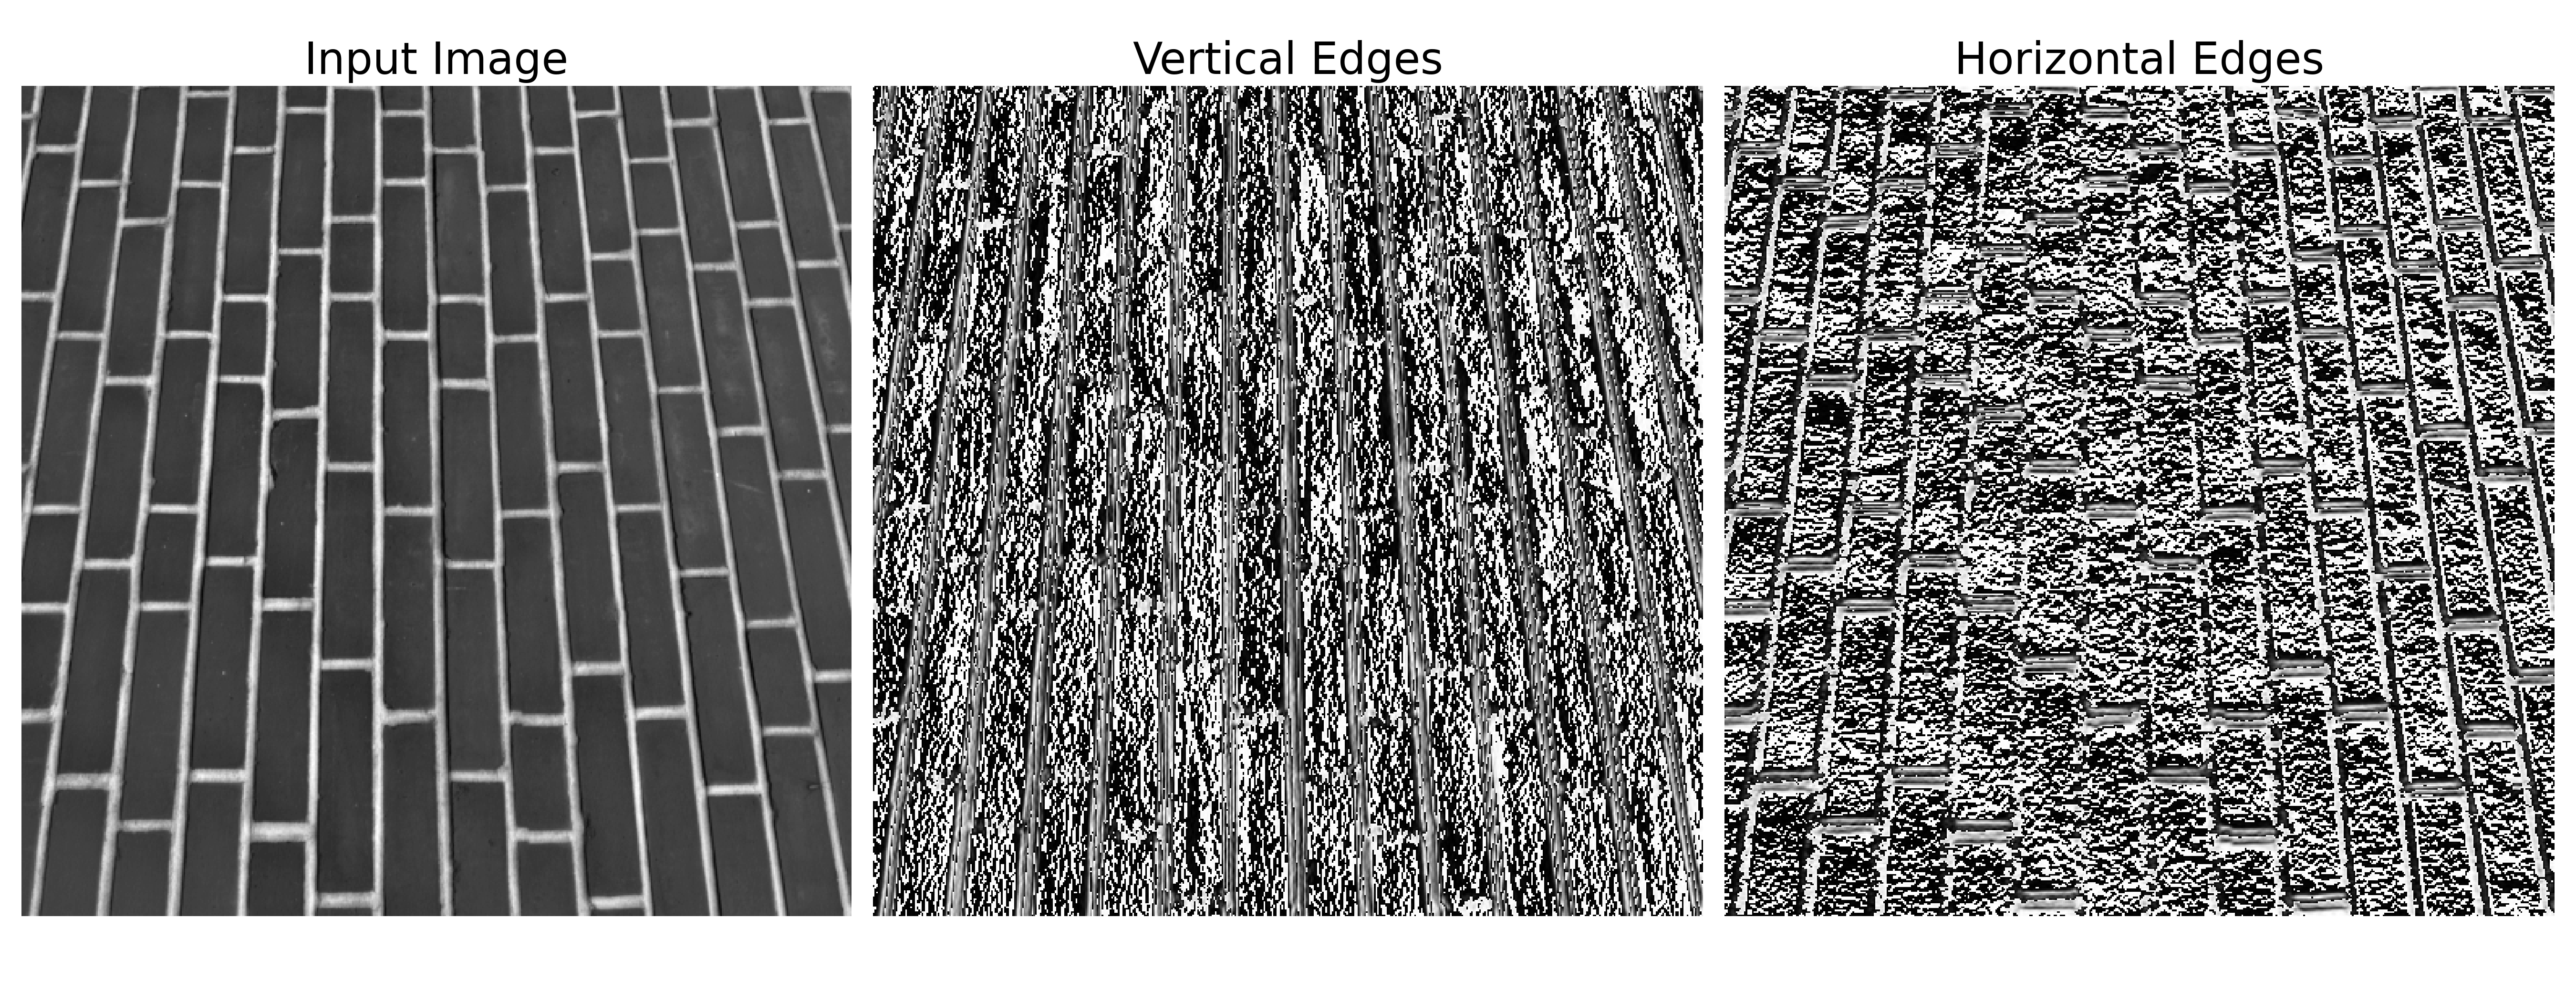
\includegraphics[width=0.9\linewidth]{img/kernels.png}
		\caption{Illustration of feature extraction using convolutions. The input image (left) is convolved with a vertical edge detection kernel (middle) and a horizontal edge detection kernel (right). The resulting feature maps highlight vertical and horizontal edges, respectively.}
		\label{fig:nn_featureextraction}
	\end{figure}
	
	\subsubsection*{Sparse Interactions}
	In a CNN, each neuron in a layer is connected to a small region of the input known as the receptive field, rather than the entire input. This sparse connectivity ensures that the network focuses on local patterns, making the model more efficient and reducing the number of parameters compared to fully connected layers.
	
	Sparse interactions mean that a single convolutional filter (kernel) is applied locally, which allows the network to learn spatial hierarchies. For instance, in an image, lower layers might learn to detect simple features such as edges or textures, while higher layers might combine these features to detect more complex patterns like shapes or objects. By limiting the connections to a local region, CNNs can efficiently capture spatial dependencies.
	
	\paragraph{Benefits of Sparse Interactions}
	\begin{itemize}
		\item \textbf{Efficiency}: Sparse interactions significantly reduce the number of parameters in the model. For a typical fully connected layer with \(n\) input units and \(m\) output units, there are \(n \times m\) parameters. In contrast, a convolutional layer with a filter size of \(k \times k\) applied to an \(n \times n\) input has \(k^2\) parameters per filter. Since CNNs typically use multiple filters, the number of parameters is \( k^2 \times f \), where \( f \) is the number of filters. This is still much smaller and depends only on the filter size and the number of filters, not the input size.
		\item \textbf{Parameter Sharing}: The same filter (set of parameters) is applied across different regions of the input, which allows the network to detect the same feature in different parts of the input. This parameter sharing leads to better generalization and reduces the risk of overfitting.
		\item \textbf{Local Receptive Fields}: Each neuron only focuses on a small region of the input, which enables the network to learn local features effectively. This local focus is crucial for tasks like image recognition, where spatial hierarchies are essential.
	\end{itemize}
	
	\textbf{Example:} Consider an input image of size 32x32 pixels. A convolutional layer with a 5x5 filter scans across the image, creating a feature map. Each neuron in this feature map is connected to a 5x5 region of the input image, resulting in a sparse interaction. If the filter moves one pixel at a time (stride of 1), the feature map will have a size of 28x28 (since the filter cannot go beyond the boundaries of the image without padding). This localized interaction helps the network learn relevant features while keeping the number of parameters low.\\
	
	By leveraging sparse interactions, CNNs are able to efficiently process high-dimensional data such as images, learning hierarchical features that are essential for complex pattern recognition tasks.
	
	\subsubsection*{Receptive Field}
	The receptive field refers to the region of the input that a particular neuron is responsive to. In a CNN, neurons in a layer are connected only to a small, localized region of the input, known as the receptive field. As the network goes deeper, the receptive field increases, allowing the network to capture more complex and abstract features \cite{osheaIntroductionConvolutionalNeural2015}.
	
	For example, in the first convolutional layer, each neuron might be connected to a 3x3 region of the input image (as shown in Figure \ref{fig:nn_receptivefield}). As we add more convolutional layers, the receptive field of neurons in higher layers becomes larger. This means that each neuron in these deeper layers is influenced by a larger portion of the original input image. Consequently, the network can learn hierarchical features, starting with simple edges and textures in the early layers and moving to more complex patterns and objects in the deeper layers.
	
	\begin{figure}[h]
		\centering
		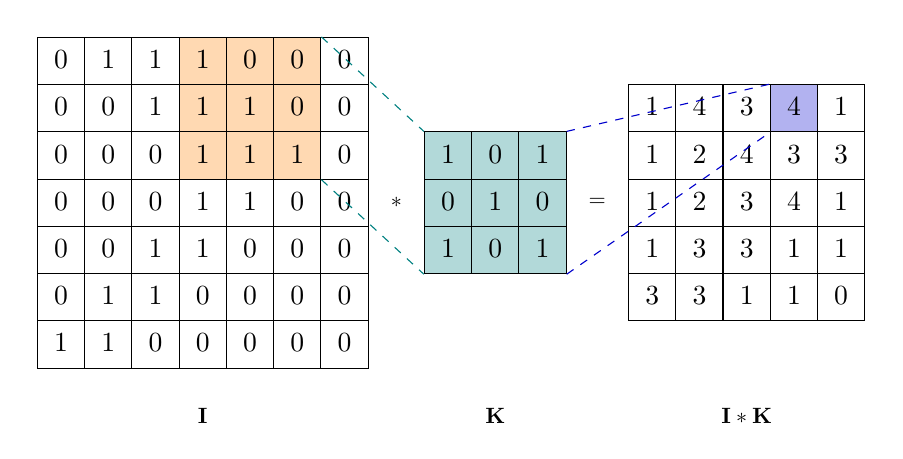
\begin{tikzpicture}[
			scale=0.8, transform shape,
			2d-arr/.style={matrix of nodes, row sep=-\pgflinewidth, column sep=-\pgflinewidth, nodes={draw, anchor=center, minimum size=0.6cm, text height=1.5ex, text depth=.25ex}}
			]
			
			\matrix (mtr) [2d-arr] {
				0 & 1 & 1 & |[fill=orange!30]| 1 & |[fill=orange!30]| 0 & |[fill=orange!30]| 0 & 0\\
				0 & 0 & 1 & |[fill=orange!30]| 1 & |[fill=orange!30]| 1 & |[fill=orange!30]| 0 & 0\\
				0 & 0 & 0 & |[fill=orange!30]| 1 & |[fill=orange!30]| 1 & |[fill=orange!30]| 1 & 0\\
				0 & 0 & 0 & 1 & 1 & 0 & 0\\
				0 & 0 & 1 & 1 & 0 & 0 & 0\\
				0 & 1 & 1 & 0 & 0 & 0 & 0\\
				1 & 1 & 0 & 0 & 0 & 0 & 0\\
			};
			
			\node[below=of mtr-5-4, yshift=-1cm] {$\mathbf I$};
			
			\node[right=0.2em of mtr] (str) {$*$};
			
			\matrix (K) [2d-arr, right=0.2em of str, nodes={draw, fill=teal!30}] {
				1 & 0 & 1 \\
				0 & 1 & 0 \\
				1 & 0 & 1 \\
			};
			\node[below=of K-3-2, yshift=-1cm] {$\mathbf K$};
			
			\node[right=0.2em of K] (eq) {$=$};
			
			\matrix (ret) [2d-arr, right=0.2em of eq] {
				1 & 4 & 3 & |[fill=blue!80!black!30]| 4 & 1\\
				1 & 2 & 4 & 3 & 3\\
				1 & 2 & 3 & 4 & 1\\
				1 & 3 & 3 & 1 & 1\\
				3 & 3 & 1 & 1 & 0\\
			};
			\node[below=of ret-4-3, yshift=-1cm] {$\mathbf{I * K}$};
			
			\draw[dashed, teal] (mtr-1-6.north east) -- (K-1-1.north west);
			\draw[dashed, teal] (mtr-3-6.south east) -- (K-3-1.south west);
			
			\draw[dashed, blue!80!black] (K-1-3.north east) -- (ret-1-4.north west);
			\draw[dashed, blue!80!black] (K-3-3.south east) -- (ret-1-4.south west);
		\end{tikzpicture}
		\caption{Visualization of a 2D convolution in a CNN. The input matrix \( \mathbf{I} \) (left) is convolved with a 3x3 kernel \( \mathbf{K} \) (center) to produce the output matrix \( \mathbf{I * K} \) (right). The orange-highlighted region in \( \mathbf{I} \) corresponds to the receptive field for the blue-highlighted element in \( \mathbf{I * K} \). Dashed lines indicate the alignment and contribution of the kernel to the output value.}
		\label{fig:nn_receptivefield}
	\end{figure}
	
	\subsubsection*{Pooling Layers}
	Pooling layers are a critical component of CNNs. They perform downsampling operations that reduce the spatial dimensions (width and height) of the input feature maps while retaining important features \cite{nirthikaPoolingConvolutionalNeural2022}. Pooling serves several key purposes in CNNs:
	\begin{itemize}
		\item \textbf{Dimensionality Reduction:} By reducing the spatial dimensions of the feature maps, pooling layers decrease the number of parameters and computational complexity of the model. This makes the network more efficient and faster to train.
		\item \textbf{Translation Invariance:} Pooling helps the network to become more robust to translations and distortions in the input data. By summarizing local regions, it ensures that small shifts or changes in the input do not significantly affect the output.
		\item \textbf{Overfitting Reduction:} By reducing the number of parameters, pooling layers help to prevent overfitting, especially when working with smaller datasets.
	\end{itemize}
	
	\paragraph{Common Pooling Methods}:
	\begin{itemize}
		\item \textbf{Max Pooling:} Max pooling selects the maximum value within a local patch of the feature map. It effectively retains the most prominent features in the local region.
		\begin{equation*}
			y_{i,j} = \max \left( x_{i+k,j+l} \right), \quad \forall \, 0 \leq k,l < f
		\end{equation*}
		where \( f \) is the filter size, and \( x \) is the input feature map.
		
		\item \textbf{Average Pooling:} Average pooling computes the average value within a local patch of the feature map. It smooths the feature map and reduces noise by averaging the values.
		\begin{equation*}
			y_{i,j} = \frac{1}{f^2} \sum_{k=0}^{f-1} \sum_{l=0}^{f-1} x_{i+k,j+l}
		\end{equation*}
		
		\item \textbf{Pooling via Convolutional Layers:} Pooling via convolutional layers, often referred to as strided convolutions, involves using a convolutional layer with a stride greater than one. This method applies a convolution operation but skips over certain elements of the input feature map, effectively reducing its dimensionality. Pooling via convolutional layers allows the network to learn the pooling operation itself, potentially capturing more complex patterns compared to traditional pooling methods.
	\end{itemize}
	
	\textbf{Example}: Consider a 4x4 feature map that we apply 2x2 max pooling to with a stride of 2. The resulting 2x2 feature map will contain the maximum values from each 2x2 patch of the input feature map. This process reduces the spatial dimensions by a factor of 2 while preserving the most significant features.
	
	In summary, pooling layers play a crucial role in reducing the spatial dimensions of feature maps, enhancing computational efficiency, and promoting translation invariance in convolutional neural networks. The most commonly used pooling methods are max pooling and average pooling, each with its own advantages depending on the application.
	
	\subsubsection*{Fully Connected Layers in CNNs}
	After several convolutional and pooling layers, CNNs typically include fully connected layers. These layers integrate the features learned by the convolutional layers to make the final prediction, and perform duties similar to layers in standard neural networks \cite{osheaIntroductionConvolutionalNeural2015}.
	
	\subsection*{Feature importance in CNNs}
	The theoretical aspects of CNNs presented so far, are implemented to identify and utilize the most relevant parts of the input data to make predictions. This involves the previously mentioned use of convolutional layers to apply filters and produce feature maps, activation functions to introduce non-linearity, and pooling layers to reduce the spatial dimensions of the feature maps while retaining important information. Fully connected layers then use these extracted features for final classification or prediction tasks. Effective feature extraction is critical for the performance and interpretability of CNN models. Visualizing the importance of features enhance the interpretability of CNN models by highlighting which parts of the input data are most influential in making predictions. Two prominent methods for feature importance visualization are Shapley values and Gradient-weighted Class Activation Mapping (GradCAM), each offering unique approaches to understanding and visualizing model decisions.
	
	\subsubsection*{Shapley Values for Feature Attributions}
	Shapley values provide a fair and theoretically grounded method for attributing the contribution of each feature to a model's prediction. By considering the marginal contribution of each feature across all possible subsets, Shapley values help identify which features are most influential in the model's decision-making process. This approach is particularly valuable in understanding the underlying biological mechanisms in complex tasks such as predicting antimicrobial resistance \cite{wrobelEfficientExplanationIndividual}.
	
	\subsubsection*{GradCAM for Visual Explanations}
	GradCAM is a technique that generates visual explanations for decisions made by CNN-based models. By using the gradients flowing into the final convolutional layer, GradCAM produces localization maps that highlight the important regions in the input for predicting a specific class. This method enhances the interpretability of CNNs, making it easier to understand and trust their predictions in applications such as image classification and  resistance predictions \cite{selvarajuGradCAMVisualExplanations2020}.
		
\clearpage
\section*{Methods}
	Different methodologies were employed for predicting species and resistances, and these will be described in their respective sections. However, common practices were followed for both methodologies. Specifically, Python (version 3.11) \cite{python} was used as the programming language, and all computations were performed on the GenomeDK cluster (\url{genome.au.dk}) at Aarhus University.

	Figure \ref{fig:workflow} illustrates the workflow of the analysis process, highlighting the distinct paths taken for species classification and resistance classification, encompassing filtering, splitting, modeling, and evaluation stages.

	
	\begin{figure}[h!]
		\centering
		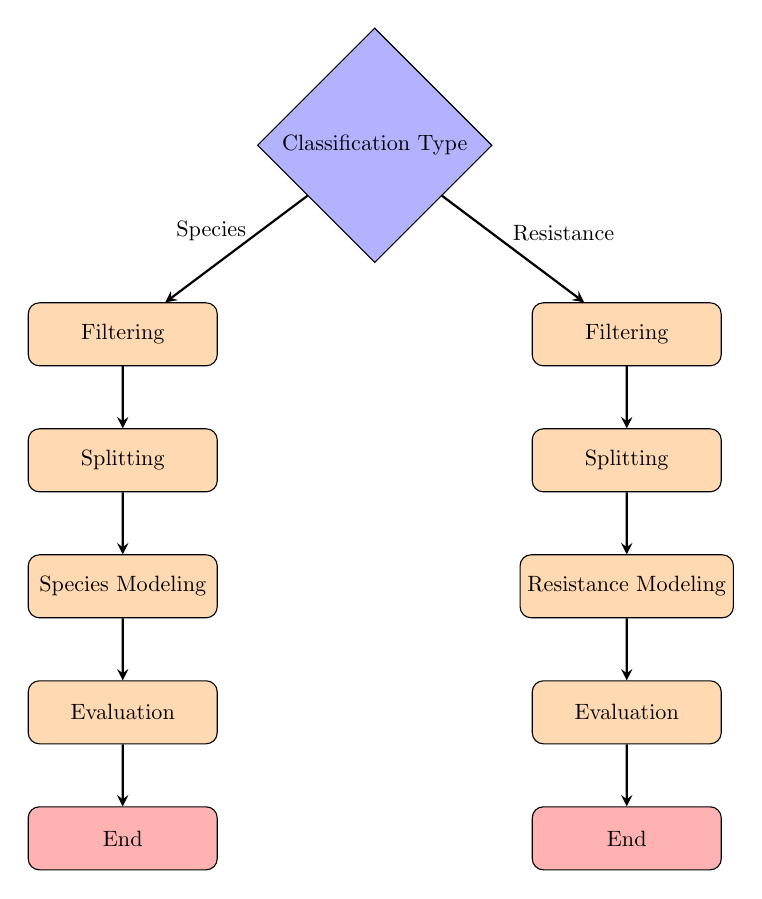
\begin{tikzpicture}[node distance=2cm and 3cm,scale=0.8, transform shape,]
			% Nodes
			\node (decision) [decision] {Classification Type};
			
			\node (species_filter) [process, below of=decision, xshift=-4cm, yshift=-1cm] {Filtering};
			\node (species_split) [process, below of=species_filter] {Splitting};
			\node (species_model) [process, below of=species_split] {Species Modeling};
			\node (species_evaluate) [process, below of=species_model] {Evaluation};
			\node (species_end) [startstop, below of=species_evaluate] {End};
			
			\node (resistance_filter) [process, below of=decision, xshift=4cm, yshift=-1cm] {Filtering};
			\node (resistance_split) [process, below of=resistance_filter] {Splitting};
			\node (resistance_model) [process, below of=resistance_split] {Resistance Modeling};
			\node (resistance_evaluate) [process, below of=resistance_model] {Evaluation};
			\node (resistance_end) [startstop, below of=resistance_evaluate] {End};
			
			% Arrows			
			\draw [arrow] (decision) -- node[anchor=south, xshift=-0.4cm] {Species} (species_filter);
			\draw [arrow] (species_filter) -- (species_split);
			\draw [arrow] (species_split) -- (species_model);
			\draw [arrow] (species_model) -- (species_evaluate);
			\draw [arrow] (species_evaluate) -- (species_end);
			
			\draw [arrow] (decision) -- node[anchor=south, xshift=0.8cm] {Resistance} (resistance_filter);
			\draw [arrow] (resistance_filter) -- (resistance_split);
			\draw [arrow] (resistance_split) -- (resistance_model);
			\draw [arrow] (resistance_model) -- (resistance_evaluate);
			\draw [arrow] (resistance_evaluate) -- (resistance_end);
		\end{tikzpicture}
		\caption{Workflow of the analysis process, showing separate paths for species classification and resistance classification, including preprocessing, filtering, splitting, modeling, and evaluation steps.}
		\label{fig:workflow}
	\end{figure}
	
	\subsection*{Species classification}
	For species classification, the data used was sourced directly from the dataset described in Weis et al. (2022) \cite{weis2021driams,weisDirectAntimicrobialResistance2022}. Specifically, the mass spectra were binned into 6000 fixed bins of 3 Da each, ranging from 2,000 Da to 20,000 Da, to create a consistent 6000-dimensional feature vector for each sample. This binning process ensures that each spectrum is uniformly represented, enabling the effective application of machine learning algorithms.
	
	The preprocessing steps involved in creating the binned data include the following, as described by Weis et al.:
	
	\begin{itemize}
		\item \textbf{Mass-to-Charge Ratio (m/z) Partitioning}: The m/z axis is divided into equal-sized bins of 3 Da.
		\item \textbf{Intensity Summation}: The intensity of all measurements falling within each bin is summed to produce the feature vector.
	\end{itemize}
	
	Prior to creating any models, the data was filtered to exclude data points that included the string "MIX!" in their species label (e.g. "MIX!Klebsiella pneumoniae"), as it was unclear how this label should be interpreted. Additionally, species containing fewer than five samples were excluded to ensure more reliable modeling. The data was then split into training (80\%) and validation (20\%) sets using a stratified split method based on species to ensure that all species were represented in both sets.
	
	All machine learning models for species classification, including elastic net, Ridge, random forest, and SVM, were implemented using scikit-learn \cite{scikit-learn}.
	
	\subsection*{Resistance classification}
	For resistance classification, the mass spectra underwent several preprocessing steps to ensure the data was suitable for model training and prediction. These preprocessing steps included log-transformation, smoothing, normalization, and rescaling, as detailed below. These steps were originally implemented in R by PhD student Johan Kjeldbjerg Lassen at Bioinformatics Research Center, Aarhus University, and had been completed prior to me beginning this project.
	
	\subsubsection*{Preprocessing steps}
	\begin{enumerate}
		\item \textbf{Log-transformation}: The intensity values of the mass spectra were log-transformed to stabilize variance and make the data more normally distributed:
		\begin{equation*}
			int_{log} = log(int + 1)
		\end{equation*}
		\item \textbf{Smoothing with LOWESS}: A two-step Locally Weighted Scatterplot Smoothing (LOWESS) procedure was applied to the log-transformed intensities:
		\begin{itemize}
			\item \textbf{First LOWESS}: Applied with a smoothing parameter \( \alpha = 0.0008 \) to smooth out the data.
			\item \textbf{Second LOWESS}: Applied with \( \alpha = 0.3 \) to further smooth and normalize the data.
		\end{itemize}
		\item \textbf{Rescaling}: The normalized intensities were rescaled to a range of \( [-1, 1] \):
		\begin{equation}
			int_{rescaled} = 2 \left( \frac{int_{normalized} - int_{min}}{int_{max} - int_{min}} \right) - 1
		\end{equation}
		\item \textbf{Mapping to new scale}: The m/z values were mapped to a new scale ranging from 2000 Da to 20000 Da with 0.5 Da increments using a final LOWESS \( \alpha = 0.0003 \).
	\end{enumerate}
	These preprocessing steps ensured that the mass spectra were uniformly represented and smoothed, reducing noise and enhancing signal clarity. A visualization of these steps is shown in Figure \ref{fig:preprocessing_steps}.
	
	\subsubsection*{Data filtering and splitting}
	In order to standardize and focus the analysis on the most prevalent resistances, I identified the top 25 most frequent resistances from each dataset in the DRIAMS-A collection using a custom Python script. The script filters out entries labeled as 'MIX!' in the species column, counts the occurrences of each resistance phenotype, and selects the most common resistances. Subsequently, the script consolidates these resistances across all datasets, retaining only those resistances in the filtered datasets, thus ensuring that the final datasets include a consistent set of the most frequent resistance phenotypes for analysis.
	
	The filtered datasets were initially divided into training/validation (90\%) and testing (10\%) sets. Due to the multilabel nature of the resistance classification problem, the split was performed using scikit-multilearn \cite{2017arXiv170201460S}, which ensures an even distribution of label combinations across the splits (as demonstrated in \ref{fig:multilabel_split}). The training/validation set was further divided into training (80\%) and validation (20\%) subsets using the same method.
	
	\subsubsection*{Model implementations}
	Ridge and random forest classification models were implemented using scikit-learn \cite{scikit-learn}. CNN models were implemented using PyTorch \cite{NEURIPS2019_9015}, PyTorch Lightning \cite{falcon2019pytorch}, and Weights and Biases \cite{wandb}.
	
	\begin{figure}[h]
		\centering
		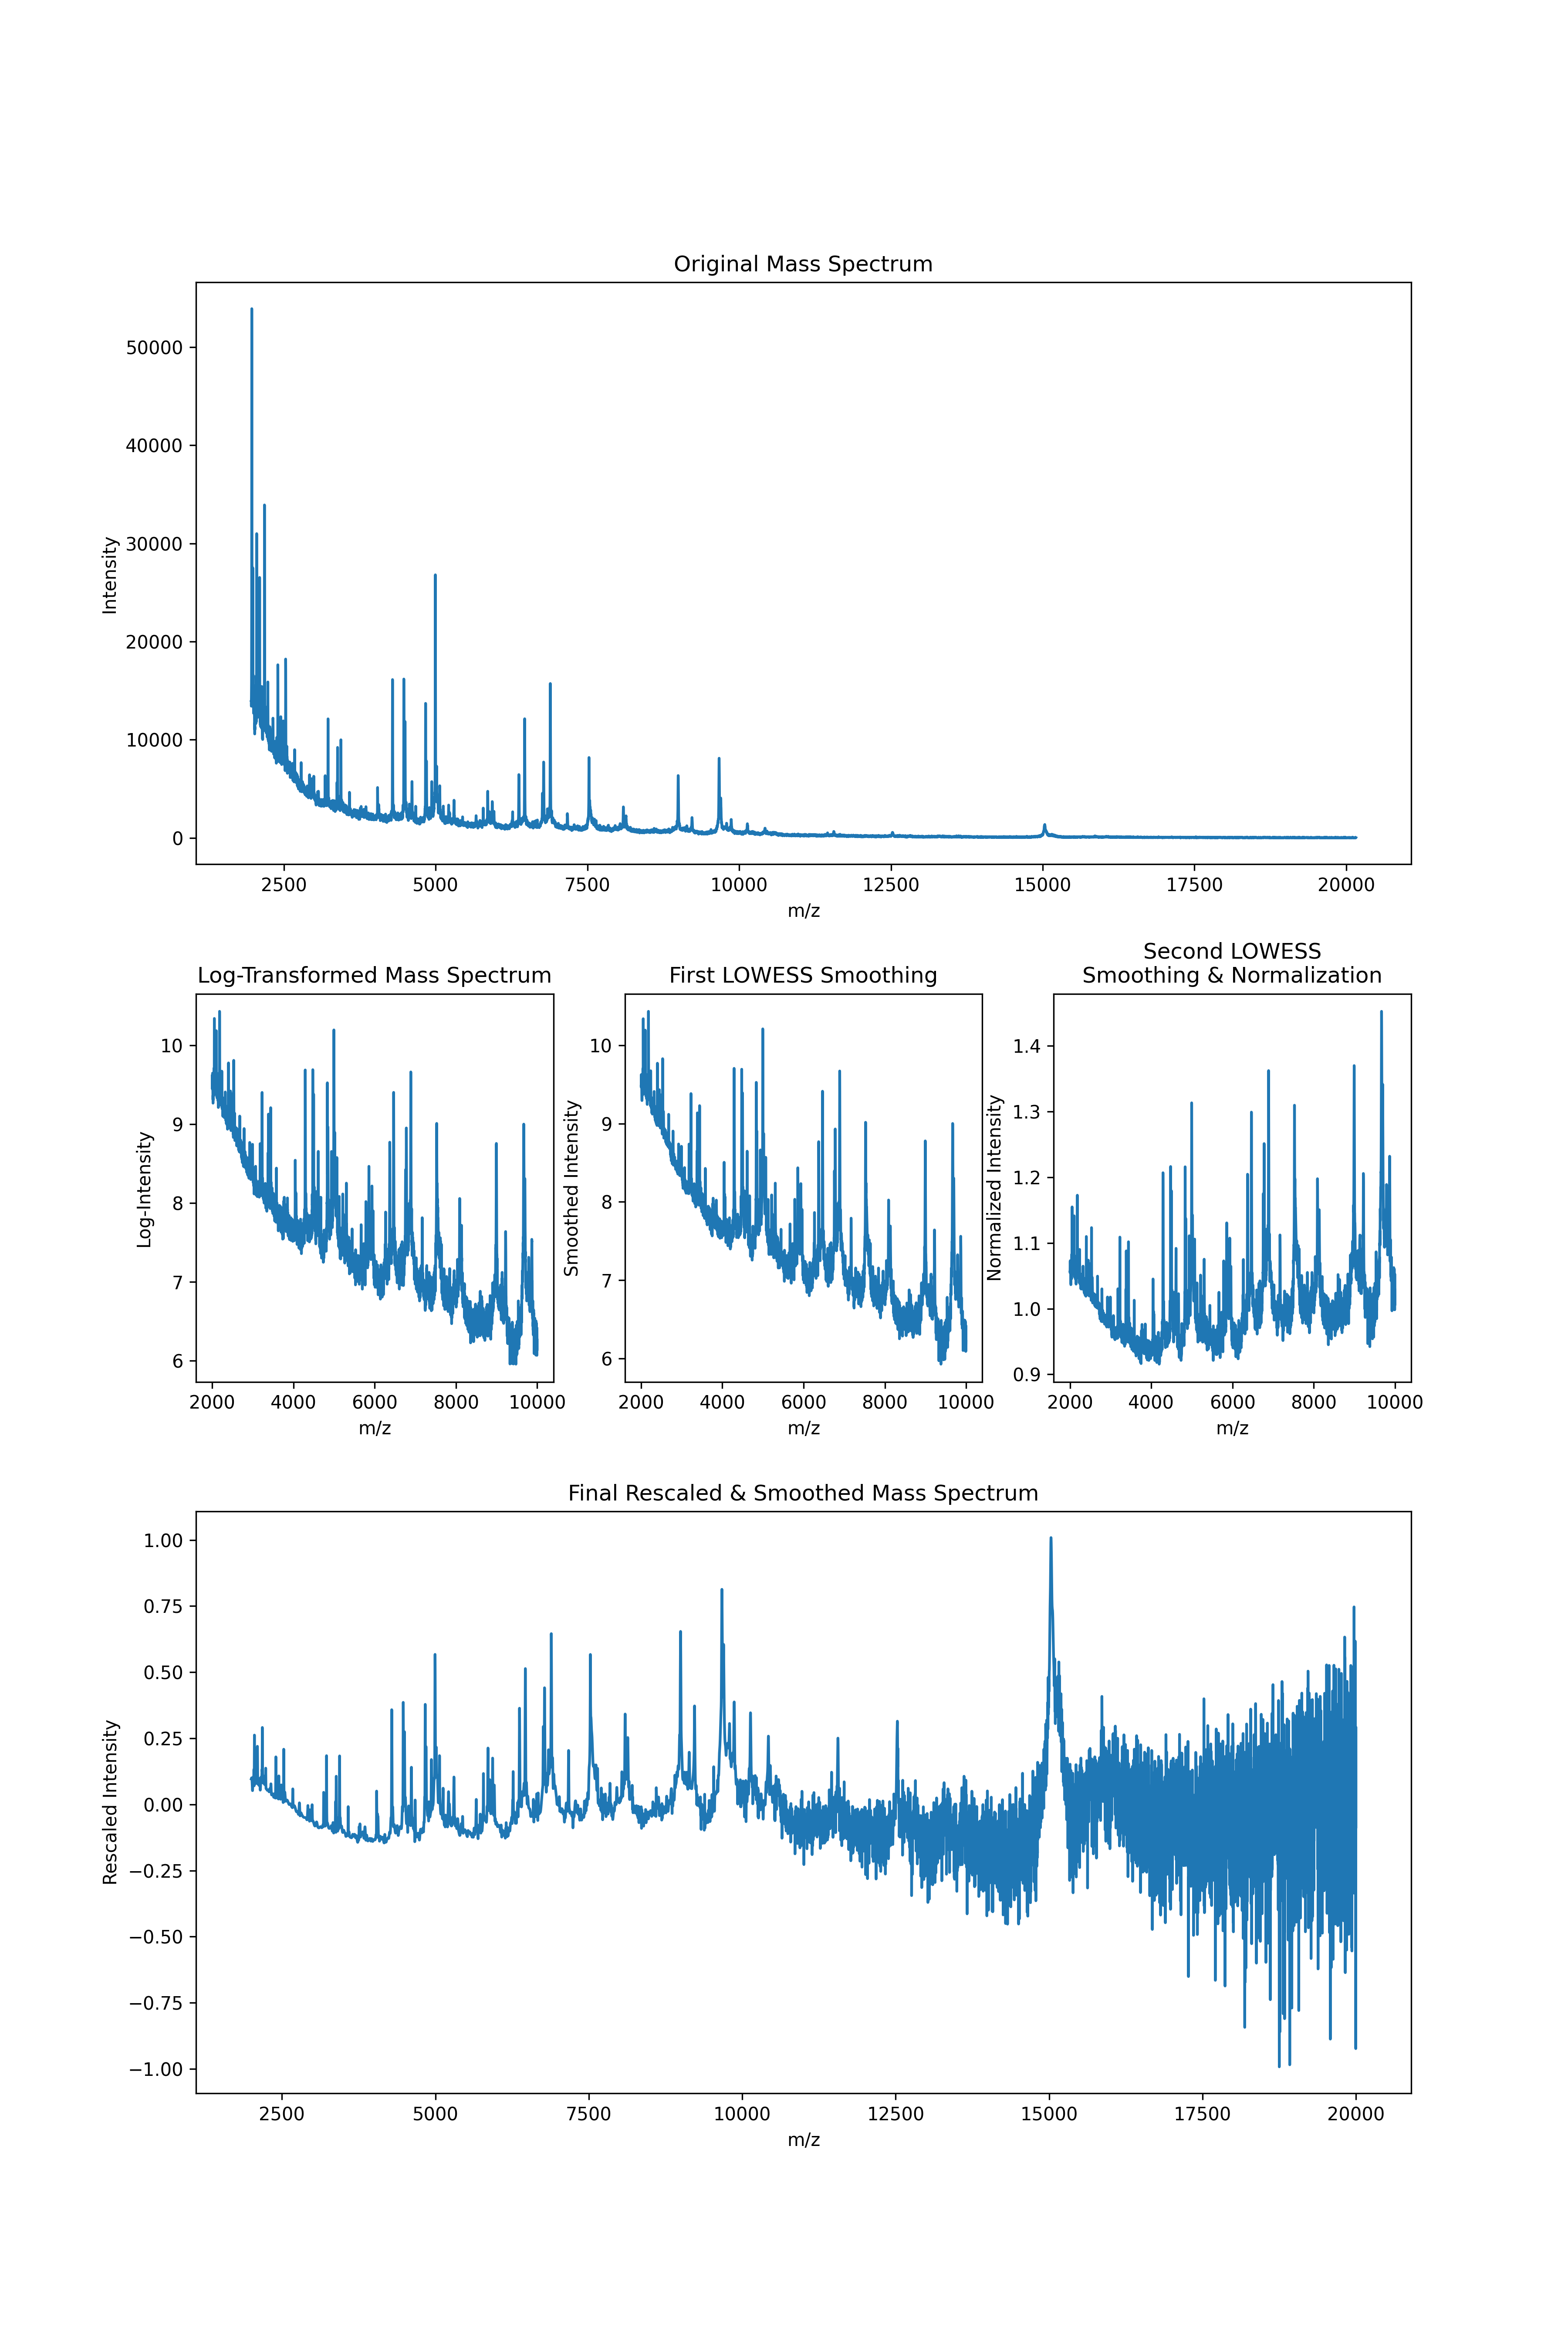
\includegraphics[width=0.9\linewidth]{img/preprocessing_steps_combined.png}
		\caption{Illustration of the preprocessing steps applied to an original MALDI-TOF mass spectrum. The top plot shows the original mass spectrum. The middle row includes three subplots displaying the intermediate steps: the log-transformed mass spectrum (left), the first LOWESS smoothing (middle), and the second LOWESS smoothing with normalization (right). The bottom plot presents the final rescaled and smoothed mass spectrum. This step-by-step preprocessing enhances the data quality by reducing noise and normalizing intensity values, facilitating more effective downstream analysis.}
		\label{fig:preprocessing_steps}
	\end{figure}
	
	\subsubsection*{Performance Metrics}
	To evaluate the effectiveness of the machine learning models implemented in this thesis, I employed different performance metrics for species classification and resistance classification.
	
	For species classification, accuracy was used as the performance metric. This is defined as the proportion of correct predictions made by the model out of the total number of predictions. This metric provides a straightforward measure of how well the model is performing in terms of correctly identifying the species from the MALDI-TOF mass spectra.
	
	For resistance classification, the Area Under the Receiver Operating Characteristic Curve (AUROC) was used as the performance metric. The ROC curve is created by plotting the true positive rate (sensitivity) against the false positive rate (1-specificity). 
	
	The Area Under the Curve (AUC) provides a single scalar value to summarize the performance of the classifier. An AUC value of 1 indicates perfect performance, while an AUC value of 0.5 suggests no discriminative power, equivalent to random guessing. Higher AUC values indicate better performance. The AUROC metric is particularly useful in evaluating the resistance classification models as it accounts for the trade-off between sensitivity and specificity, providing a comprehensive measure of the model's performance.
	
	All ROC curve plots presented in the thesis have been created from model predictions of the test set defined under "Data filtering and splitting".
	
	\begin{multicols}{2}
		\subsubsection*{CNN architecture}
		The architecture of the CNN used in this study is designed to effectively capture patterns in the MALDI-TOF mass spectra data. Batch normalization layers are used after each convolution to normalize the output and improve the stability of the network. The activation function used in each layer is the Sigmoid Linear Unit (SiLU), which introduces non-linearity to the model, allowing it to learn more complex patterns. An illustration of the model architecture is presented in Figure \ref{fig:cnn_architecture}.
		
		The architecture includes two stages of convolutional operations followed by pooling layers. The pooling layers reduce the dimensionality of the feature maps, which helps in reducing computational complexity and preventing overfitting. 
		\columnbreak
		
		\begin{figure}[H] % Use H for exact placement within multicols
			\centering
			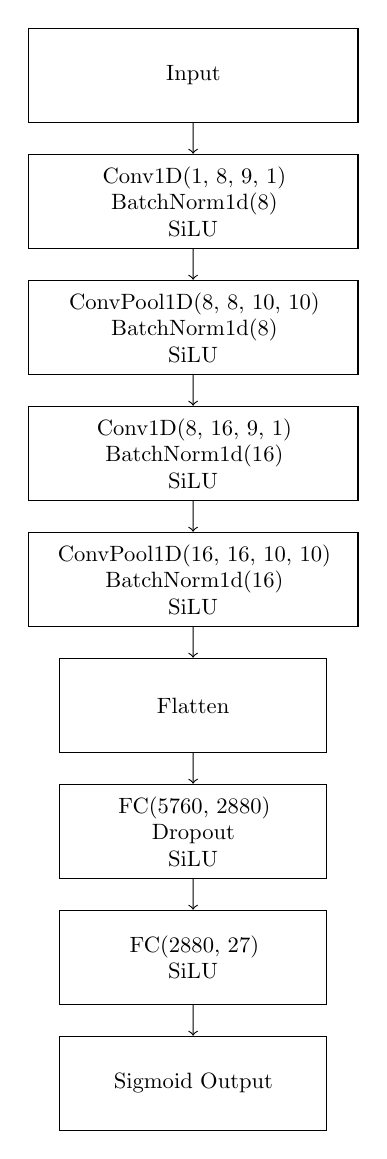
\begin{tikzpicture}[
				scale=0.8, transform shape,
				conv/.style={draw, minimum width=5cm, minimum height=1.5cm, text width=5cm, align=center},
				fc/.style={draw, minimum width=4cm, minimum height=1.5cm, text width=4cm, align=center},
				softmax/.style={draw, minimum width=4cm, minimum height=1.5cm, text width=4cm, align=center}
				]
				
				\node (input) at (0,0) [conv] {Input};
				\node (conv1) at (0,-2) [conv] {Conv1D(1, 8, 9, 1)\\ BatchNorm1d(8)\\ SiLU};
				\node (convPool1) at (0,-4) [conv] {ConvPool1D(8, 8, 10, 10)\\ BatchNorm1d(8)\\ SiLU};
				\node (conv2) at (0,-6) [conv] {Conv1D(8, 16, 9, 1)\\ BatchNorm1d(16)\\ SiLU};
				\node (convPool2) at (0,-8) [conv] {ConvPool1D(16, 16, 10, 10)\\ BatchNorm1d(16)\\ SiLU};
				\node (flatten) at (0,-10) [fc] {Flatten};
				\node (fc0) at (0,-12) [fc] {FC(5760, 2880)\\ Dropout\\ SiLU};
				\node (fc1) at (0,-14) [fc] {FC(2880, 27)\\ SiLU};
				\node (output) at (0,-16) [softmax] {Sigmoid Output};
				
				\draw[->] (input) -- (conv1);
				\draw[->] (conv1) -- (convPool1);
				\draw[->] (convPool1) -- (conv2);
				\draw[->] (conv2) -- (convPool2);
				\draw[->] (convPool2) -- (flatten);
				\draw[->] (flatten) -- (fc0);
				\draw[->] (fc0) -- (fc1);
				\draw[->] (fc1) -- (output);
			\end{tikzpicture}
			\caption{CNN Architecture}
			\label{fig:cnn_architecture}
		\end{figure}
		
	\end{multicols}
	
	Convolutional layers with increased stride are used as pooling layers. After the convolutional and pooling stages, the feature maps are flattened into a one-dimensional vector. This vector is then passed through fully connected layers (FC) which act as a classifier. Dropout is applied after the first fully connected layer to prevent overfitting by randomly setting a fraction of input units to zero during training.
	
	The final output layer uses a sigmoid activation function to output a probability for each class, indicating the presence or absence of antibiotic resistance.
	
	Using Conv1D(1, 8, 9, 1) as an example, the function's arguments from left to right are:
	\begin{itemize}
		\item \textbf{In channels:} 1 - The number of channels in the input data.
		\item \textbf{Out channels:} 8 - The number of channels produced by the convolution.
		\item \textbf{Kernel size:} 9 - The size of the convolving kernel.
		\item \textbf{Stride:} 1 - The stride of the convolution. 
	\end{itemize}
	
 	The loss function optimized during training was the \( F_{\beta} \) score \cite{leeSurrogateLossFunction2021}, which is particularly suited for imbalanced datasets by allowing the prioritization of precision or recall. The optimal \( \beta \) value was, however, found to be 1, meaning that it effectively was the \( F_1 \) score being optimized.
	
	The \( F_\beta \) Loss function can be defined as follows:
	
	\begin{equation*}
		\text{F}_\beta \text{ Loss} = 1 - \frac{(1 + \beta^2) \cdot (precision \times recall)}{(\beta^2 \cdot precision) + recall + \text{smooth}}
	\end{equation*}
	
	Where:
	\begin{align*}
		\text{precision} &= \frac{\text{true\_pos}}{\text{true\_pos} + \text{false\_pos} + \text{smooth}} \\
		\\
		\text{recall} &= \frac{\text{true\_pos}}{\text{true\_pos} + \text{false\_neg} + \text{smooth}}
	\end{align*}
	
	And:
	\begin{align*}
		\text{true\_pos} &= \sum(\text{predictions} \times \text{targets}) \\
		\text{false\_neg} &= \sum((1 - \text{predictions}) \times \text{targets}) \\
		\text{false\_pos} &= \sum(\text{predictions} \times (1 - \text{targets}))
	\end{align*}
	
	Here, $\beta$ is the beta value, and $\text{smooth}$ is a smoothing term to avoid division by zero.
	
	\subsubsection*{Feature Importance}
	To understand the contribution of different m/z ratios to the prediction of antibiotic resistance, two methods were employed: Shapley Values and GradCAM. To visualize these contributions, a representative sample for each antibiotic resistance was selected. This involved filtering the data to find instances where only one resistance phenotype was present, ensuring clear attribution. Data points where only a single resistance phenotype was present existed for 24 of the 27 resistance types, and as such it wasn't possible to generate feature importance maps for every resistance.
	
	Calculations of Shapley Values and GradCAM values were performed using the Captum \cite{kokhlikyanCaptumUnifiedGeneric} module for Python.
	
	\subsubsection*{Code Availability}
	The code used for the analyses and models presented in this thesis is available on GitHub at the following repository: \url{https://github.com/rasmusfreund/Masters-project}. This repository contains all scripts, data preprocessing steps, model training procedures, and evaluation metrics used in the study.

\section*{Results}
\subsection*{Species Classification}
\subsubsection*{Distribution of Species}
The species distribution for each year from 2015 to 2018 was analyzed using the top 10 most common species found in the dataset. The distribution of these species as a percentage of the total species count per year is shown in Figure \ref{fig:species_distribution}, illustrates the percentage distribution of each species, with each color representing a different species.. 
The top 10 species for each year were determined, and the remaining species were grouped together as "Remaining Species". The figure  The top 10 species make up \( 38.7\% \), \( 43.0\% \), \( 44.8\% \), and \( 45.9\% \) of the species in the dataset for the years 2015, 2016, 2017, and 2018, respectively.
\begin{figure}[h]
	\centering
	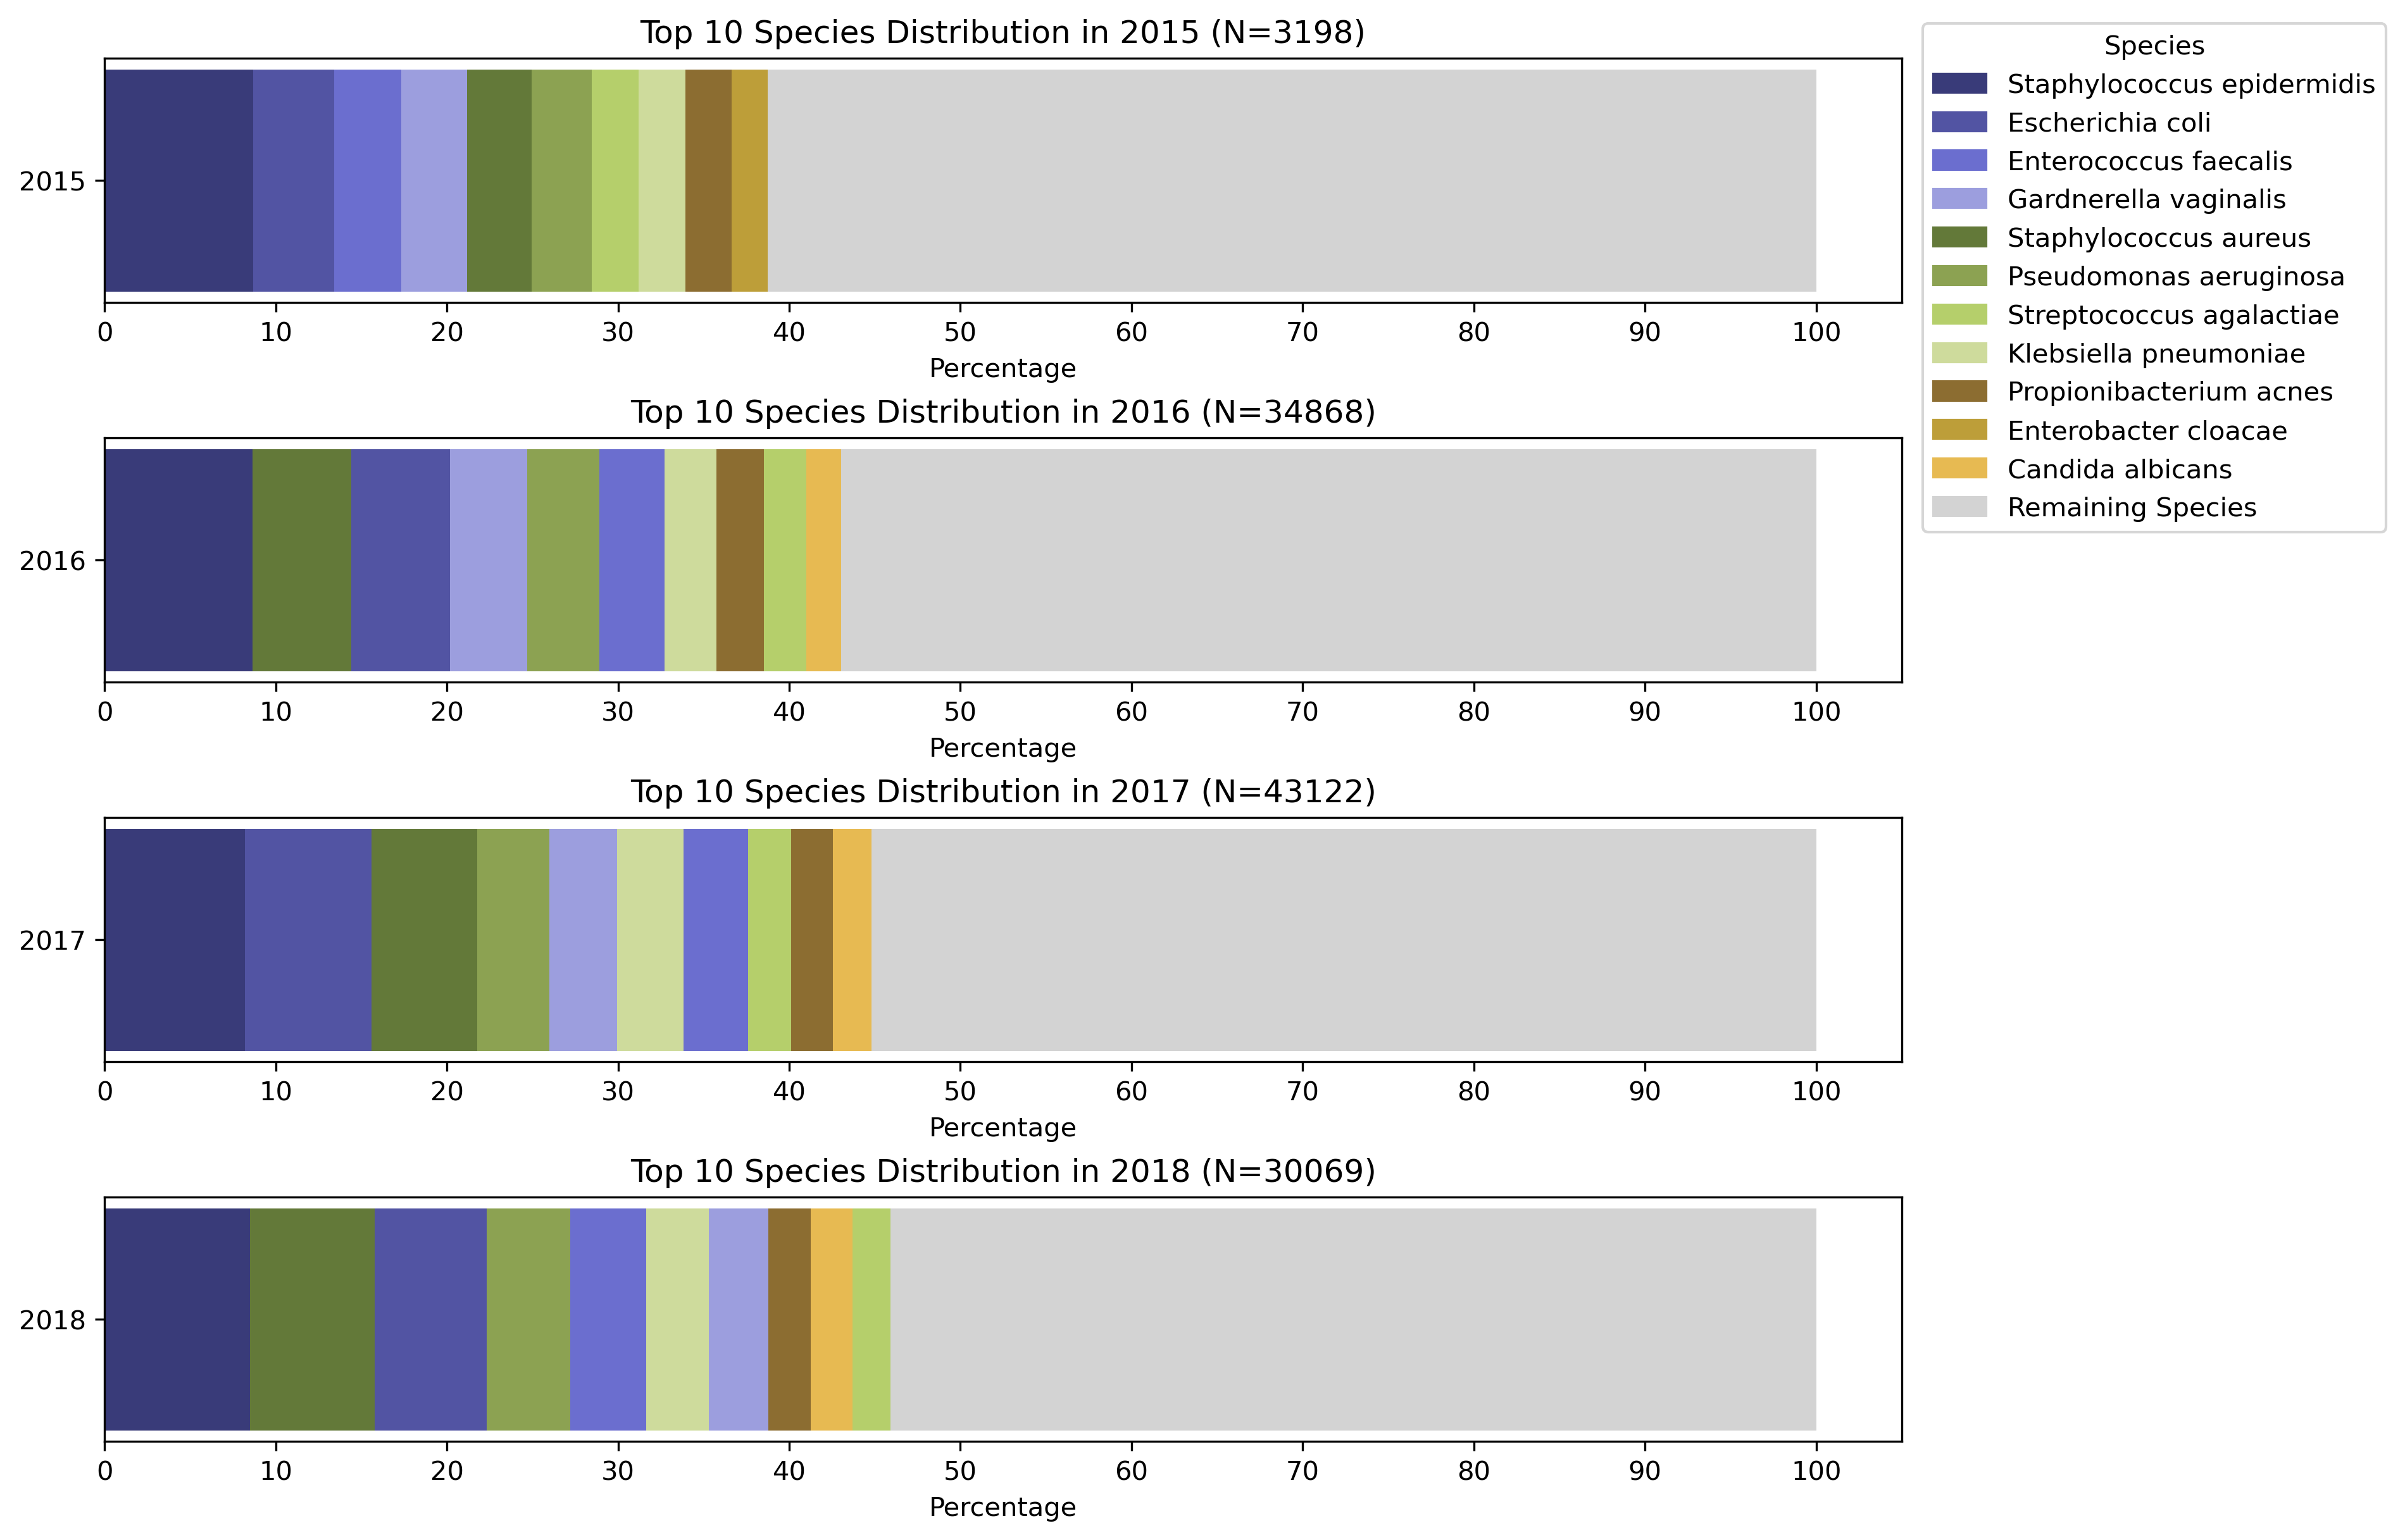
\includegraphics[width=0.9\linewidth]{img/species_distribution.png}
	\caption{Distribution of Top 10 Species from 2015 to 2018. Each bar represents the percentage of the total species count for that year, with different colors indicating different species. The legend on the right shows the species names corresponding to each color. The "Remaining Species" category includes all species not within the top 10 for each respective year.}
	\label{fig:species_distribution}
\end{figure}

\subsubsection*{Dimensionality Reduction Methods}
For both Principal Component Analysis (PCA) and Uniform Manifold Approximation and Projection (UMAP), visualizations of the dataset from the year 2017 are presented here due to it being the largest of the four datasets. Figures for the remaining three years can be found in the supplementary materials (Figures S4-S9).

PCA of the 2017 dataset, categorized by species, was performed. The top plot of Figure \ref{fig:species_pca} represents the distribution of samples based on the first two principal components (PC1 and PC2), while the bottom plot shows the distribution based on the third and fourth principal components (PC3 and PC4). Each point in the plots represents a sample, with colors indicating different species. Only the top 10 species are shown.

In the PC1 vs. PC2 plot, distinct clusters for several species are visible, suggesting that PCA has effectively captured some of the variance that separates these species. However, significant overlap between species clusters is observed, particularly for \textit{S. epidermidis} (dark blue) and \textit{S. aureus} (dark green).

The PC3 vs. PC4 plot also shows the separation of species but with different overlaps compared to the PC1 vs. PC2 plot. Clusters such as those for \textit{P. acnes} (purple) and \textit{S. agalactiae} (pink) are more dispersed, suggesting that PC3 and PC4 capture different aspects of the variance in the data.

Overall, these PCA plots demonstrate how the data can be reduced to lower dimensions while still retaining the ability to visualize the separation between different species.

\begin{figure}[h!]
	\centering
	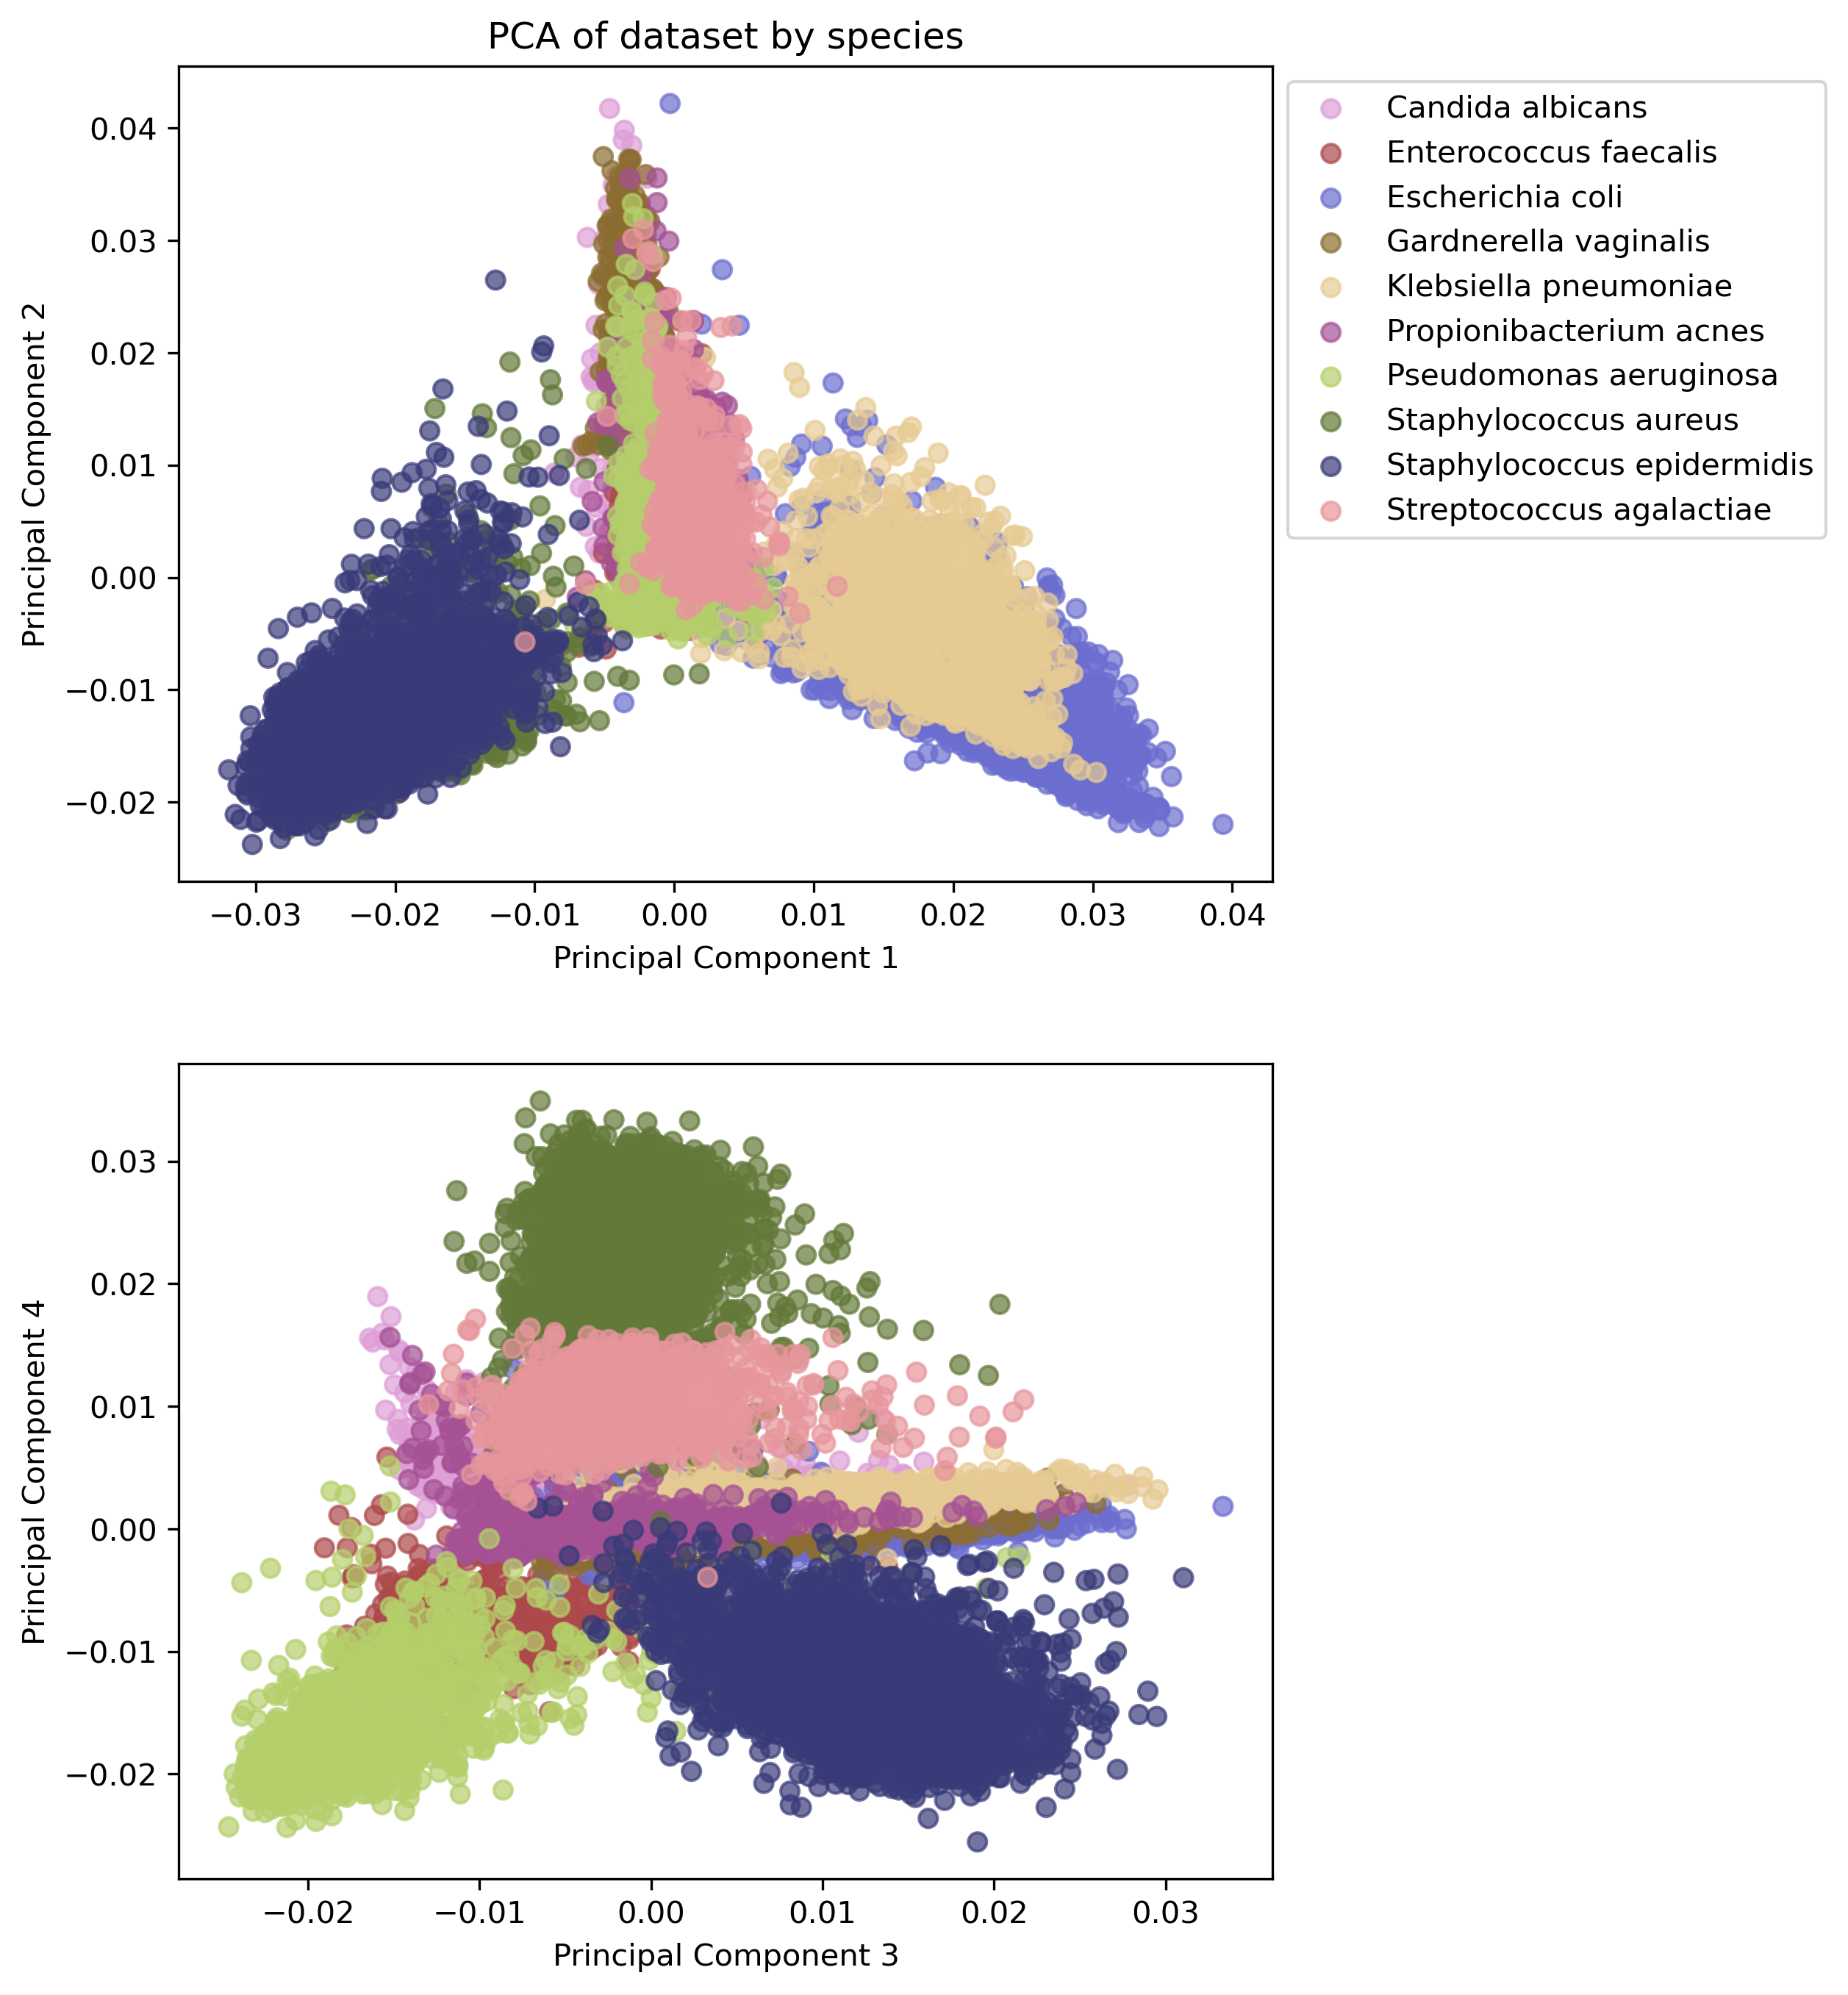
\includegraphics[width=0.9\linewidth]{img/PCA_combined.png}
	\caption{Principal Component Analysis (PCA) of the 2017 dataset by species. The top plot shows the distribution of samples based on the first two principal components (PC1 and PC2), while the bottom plot shows the distribution based on the third and fourth principal components (PC3 and PC4). Each point represents a sample, and the colors correspond to different species.}
	\label{fig:species_pca}
\end{figure}

UMAP was performed on the dataset, categorized by species. Figure \ref{fig:species_umap} illustrates the distribution of samples from the 2017 dataset in the UMAP space. Each point represents a sample, with colors indicating different species. Only the top 10 species are shown.

The UMAP plot reveals distinct clusters for several species, indicating that UMAP has effectively captured the structure of the dataset. For instance, clusters for \textit{S. epidermidis} (dark blue), \textit{S. aureus} (dark green), and \textit{E. coli} (light blue) are clearly visible.

Overall, the UMAP plot demonstrates the utility of UMAP in reducing the dimensionality of the dataset while preserving the local structure, allowing for clear visualization of species clusters.
\begin{figure}[h]
	\centering
	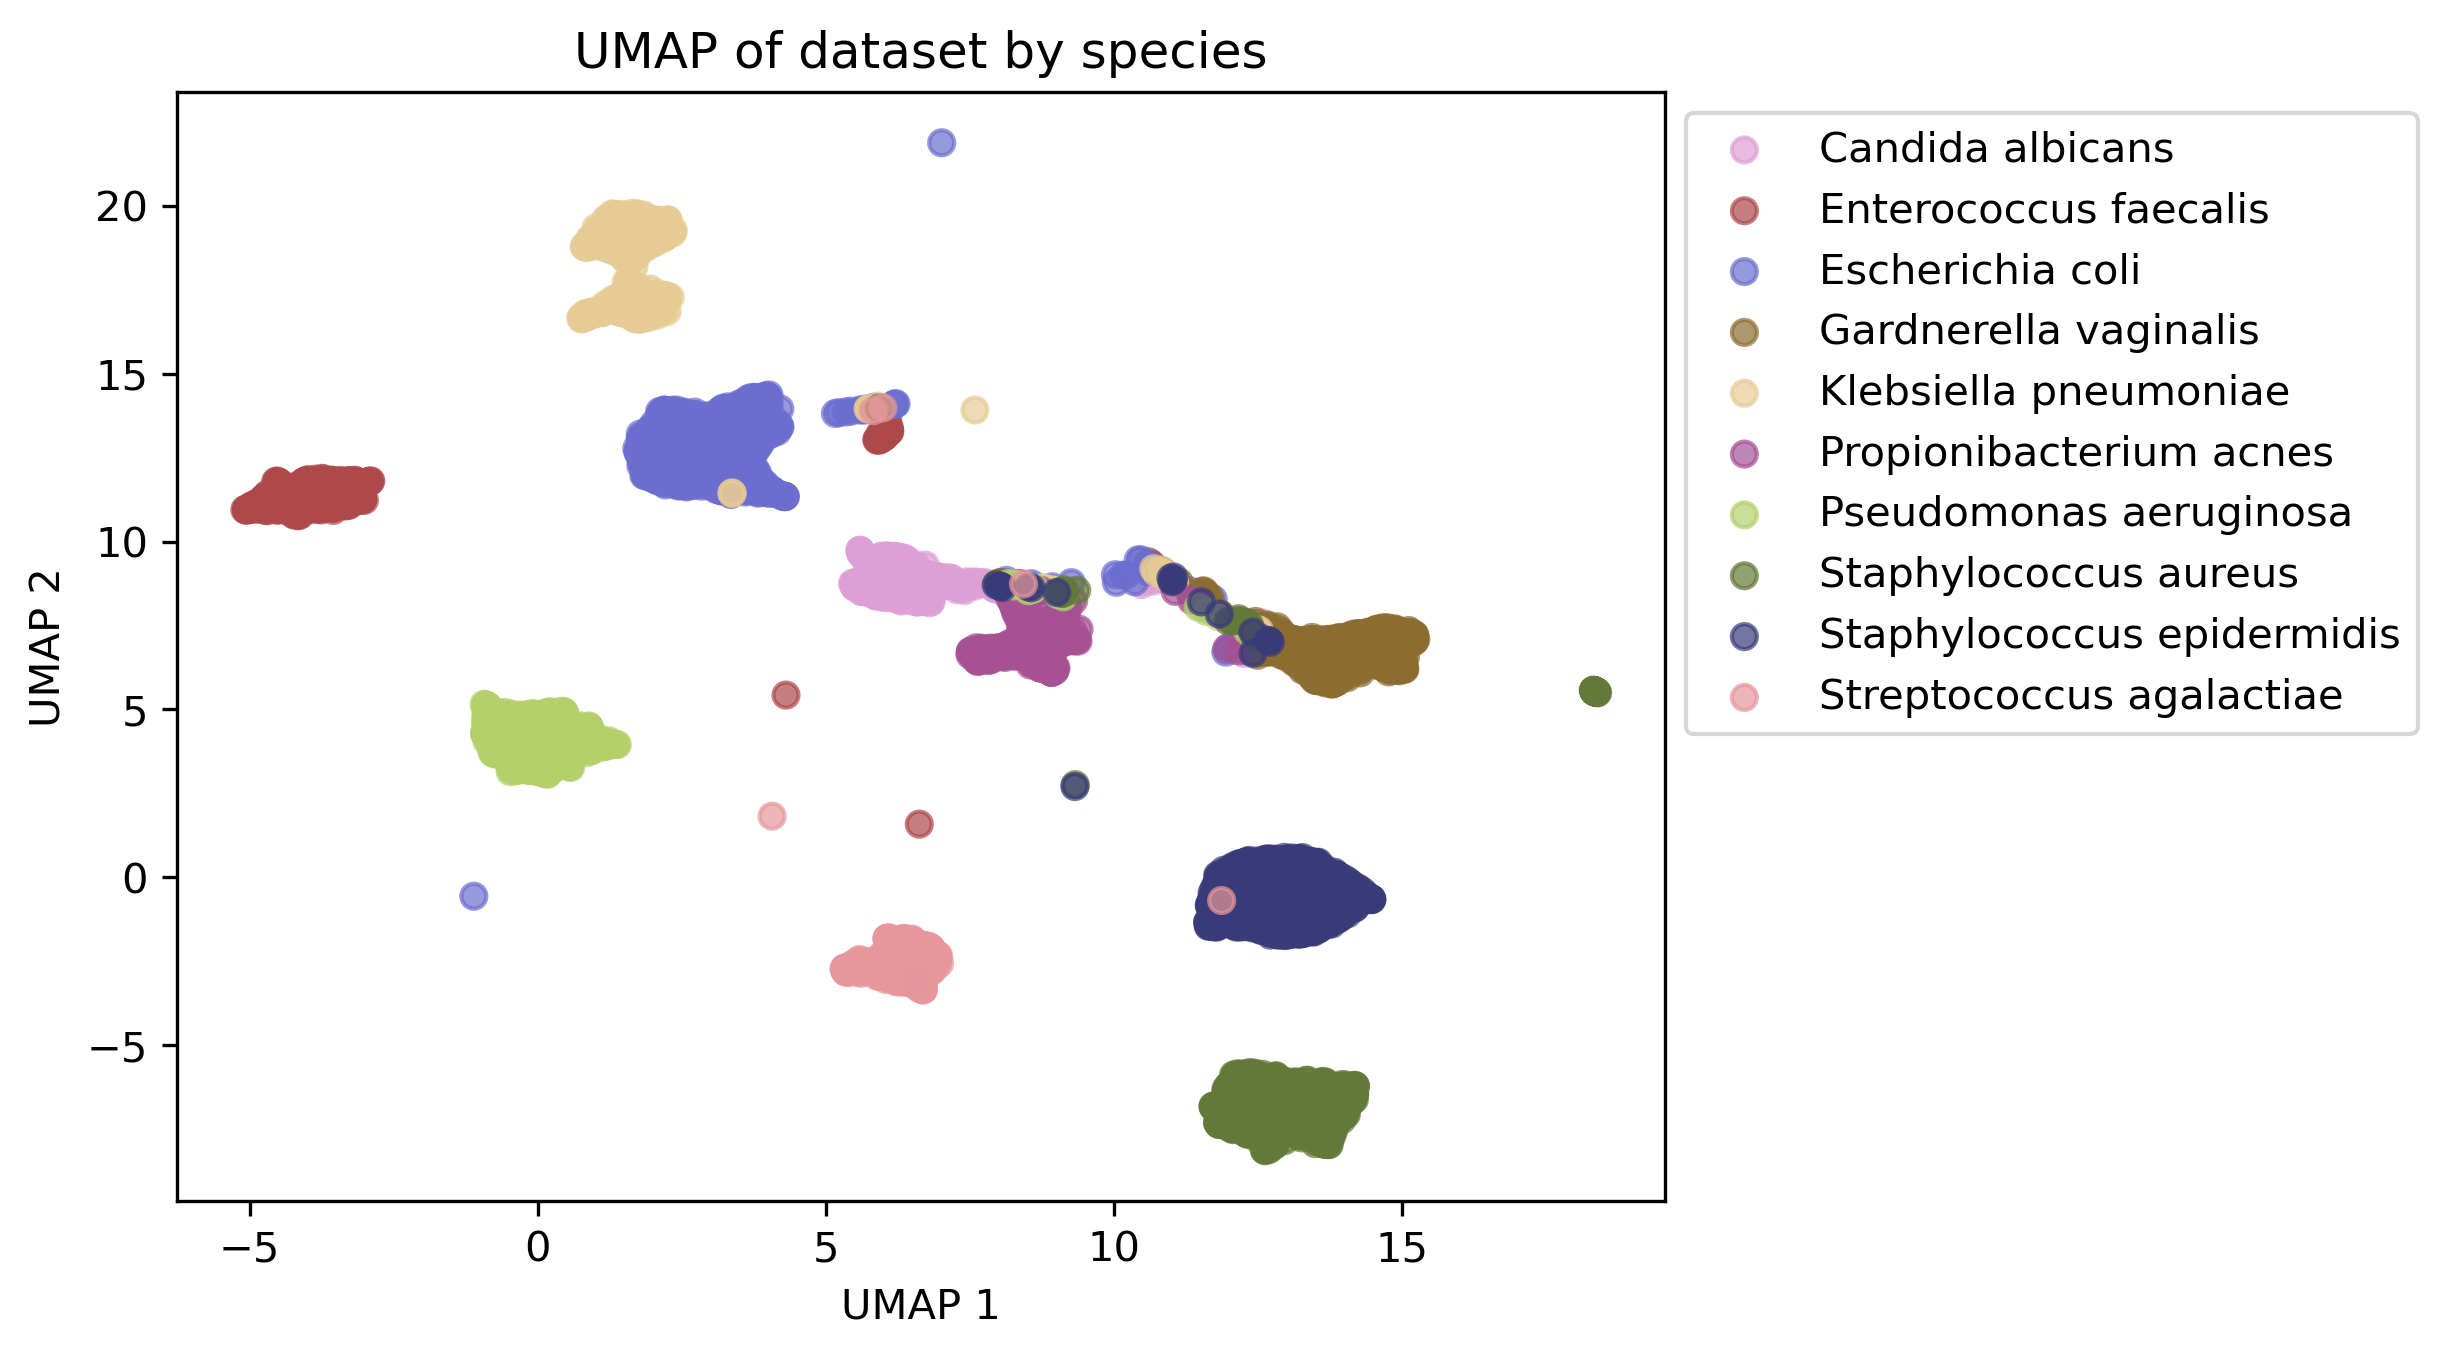
\includegraphics[width=0.9\linewidth]{img/UMAP_species_noRemaining.png}
	\caption{Uniform Manifold Approximation and Projection (UMAP) of the 2017 dataset by species. Each point represents a sample, and the colors correspond to different species. The UMAP plot reveals distinct clusters for several species, indicating effective capture of dataset structure.}
	\label{fig:species_umap}
\end{figure}

\subsubsection*{Machine Learning Model Comparison}
Figure \ref{fig:model_comparison_species} presents a comparison of the performance of four different machine learning models — Ridge, random forest, elastic net, and SVM — on predicting species from the dataset. The performance is measured in terms of mean test score (accuracy). Each point in the plot represents a five-fold cross-validation of a single hyper-parameter combination of that model for a given year. The boxplots summarize the distribution of these points for each model and year. The x-axis categorizes the data by year (2015, 2016, 2017, 2018) and includes an aggregated category for all years combined.

The plot reveals several key observations:
\begin{itemize}
	\item \textbf{Ridge}: Exhibits moderate performance across all years, with mean test scores ranging approximately between 0.2 and 0.6. There is some variability in performance, but generally, Ridge  does not achieve the highest accuracy among the models.
	\item \textbf{Random Forest}: Demonstrates relatively high and consistent performance, with mean test scores often exceeding 0.8.
	\item \textbf{Elastic Net}: Shows poor performance compared to other models, with mean test scores mostly below 0.2. This model appears to struggle with species classification.
	\item \textbf{SVM}: Achieves the highest mean test scores, often close to 1.0 for the years 2016 through 2018. SVM also shows high performance for 2015 but with slightly more variability.
\end{itemize}

Overall, the SVM model outperforms the other models, followed by random forest. Ridge regression shows moderate performance, while elastic net consistently underperforms.

\begin{figure}[h]
	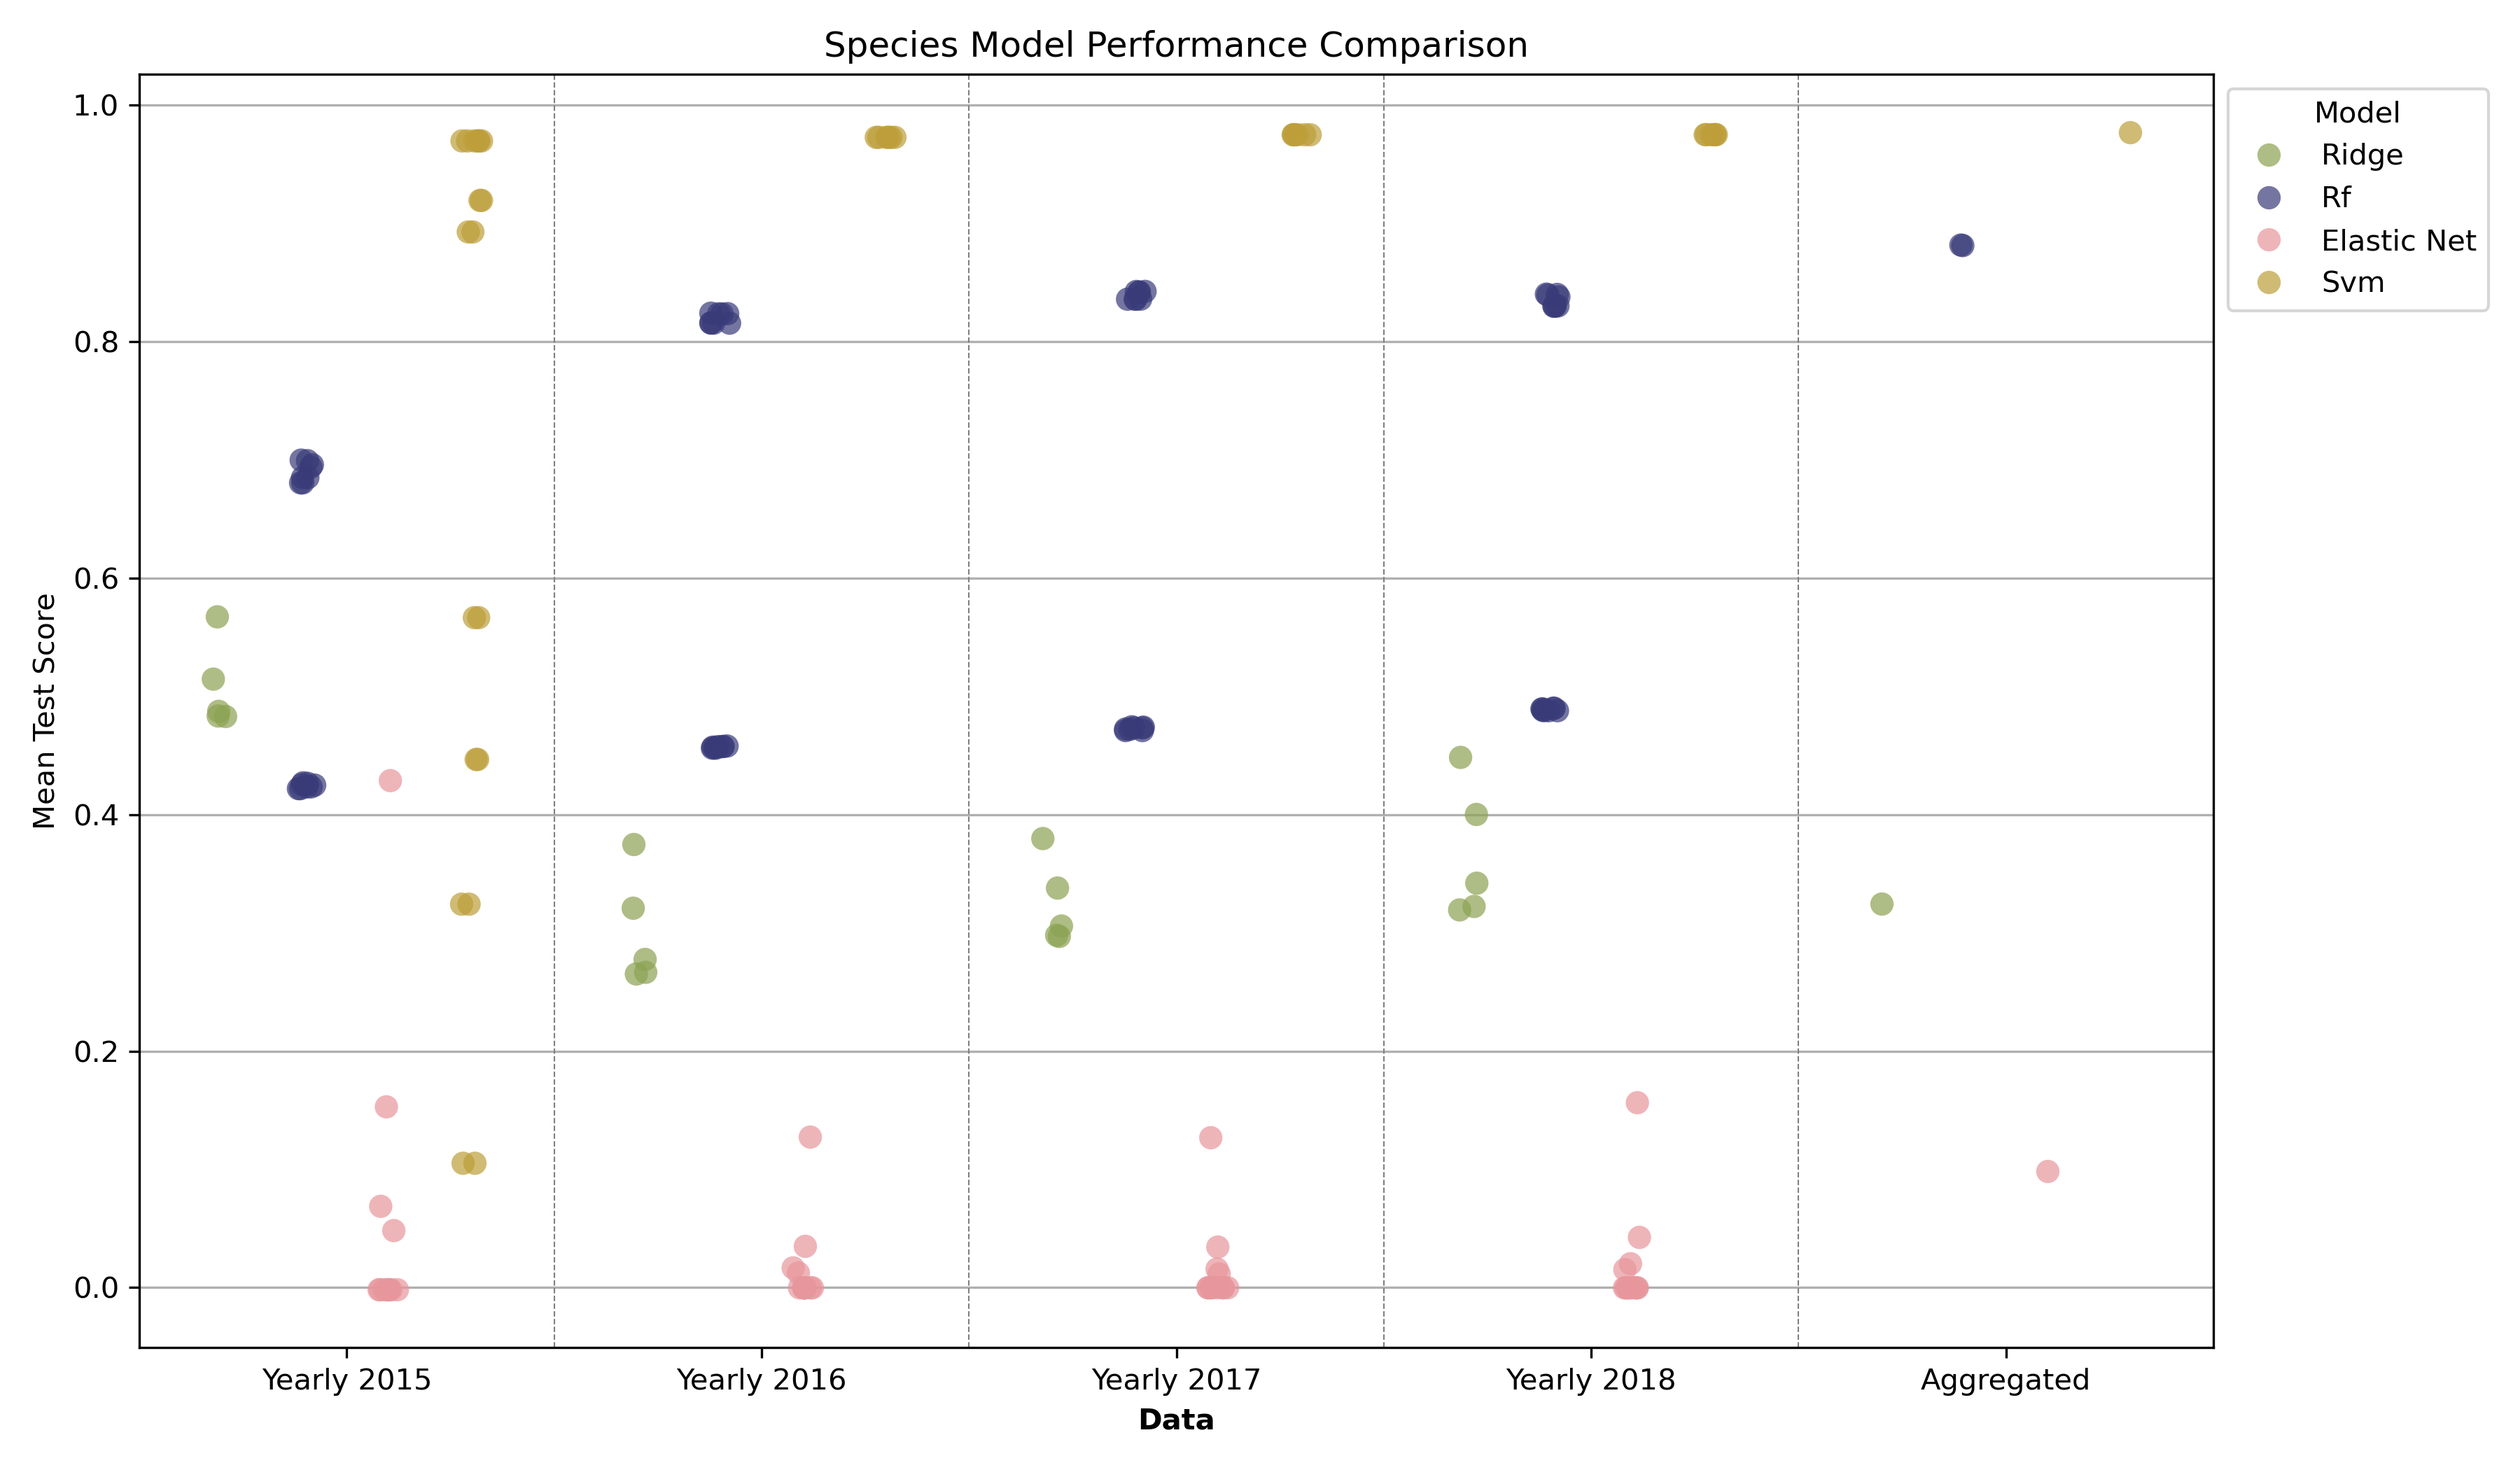
\includegraphics[width=0.9\linewidth]{img/model_comparison.png}
	\caption{Comparison of species prediction performance across different machine learning models (Ridge, random forest (RF), Elastic Net, and Support Vector Machine (SVM)). Each point represents a five-fold cross-validation of a single hyper-parameter combination for the respective model and year. The boxplots summarize the distribution of these points for each model and year, including an aggregated category for all years combined. The y-axis shows the mean test score (accuracy).}
	\label{fig:model_comparison_species}
\end{figure}

\subsection*{Antimicrobial Resistance}
For the year 2017, the antibiotic resistance distribution was visualized (Figure \ref{fig:antibiotic_resistance_distribution}), illustrating the frequency of resistance for the top 25 antibiotics across different species. The stacked bar plot represents the log-transformed frequency of resistance for each antibiotic. Each bar is divided by species, showing the contribution of each species to the overall resistance for that antibiotic. Within each bar, species are sorted by their frequency of resistance, with species contributing fewer samples placed lower in the bar.

\begin{figure}[h]
	\centering
	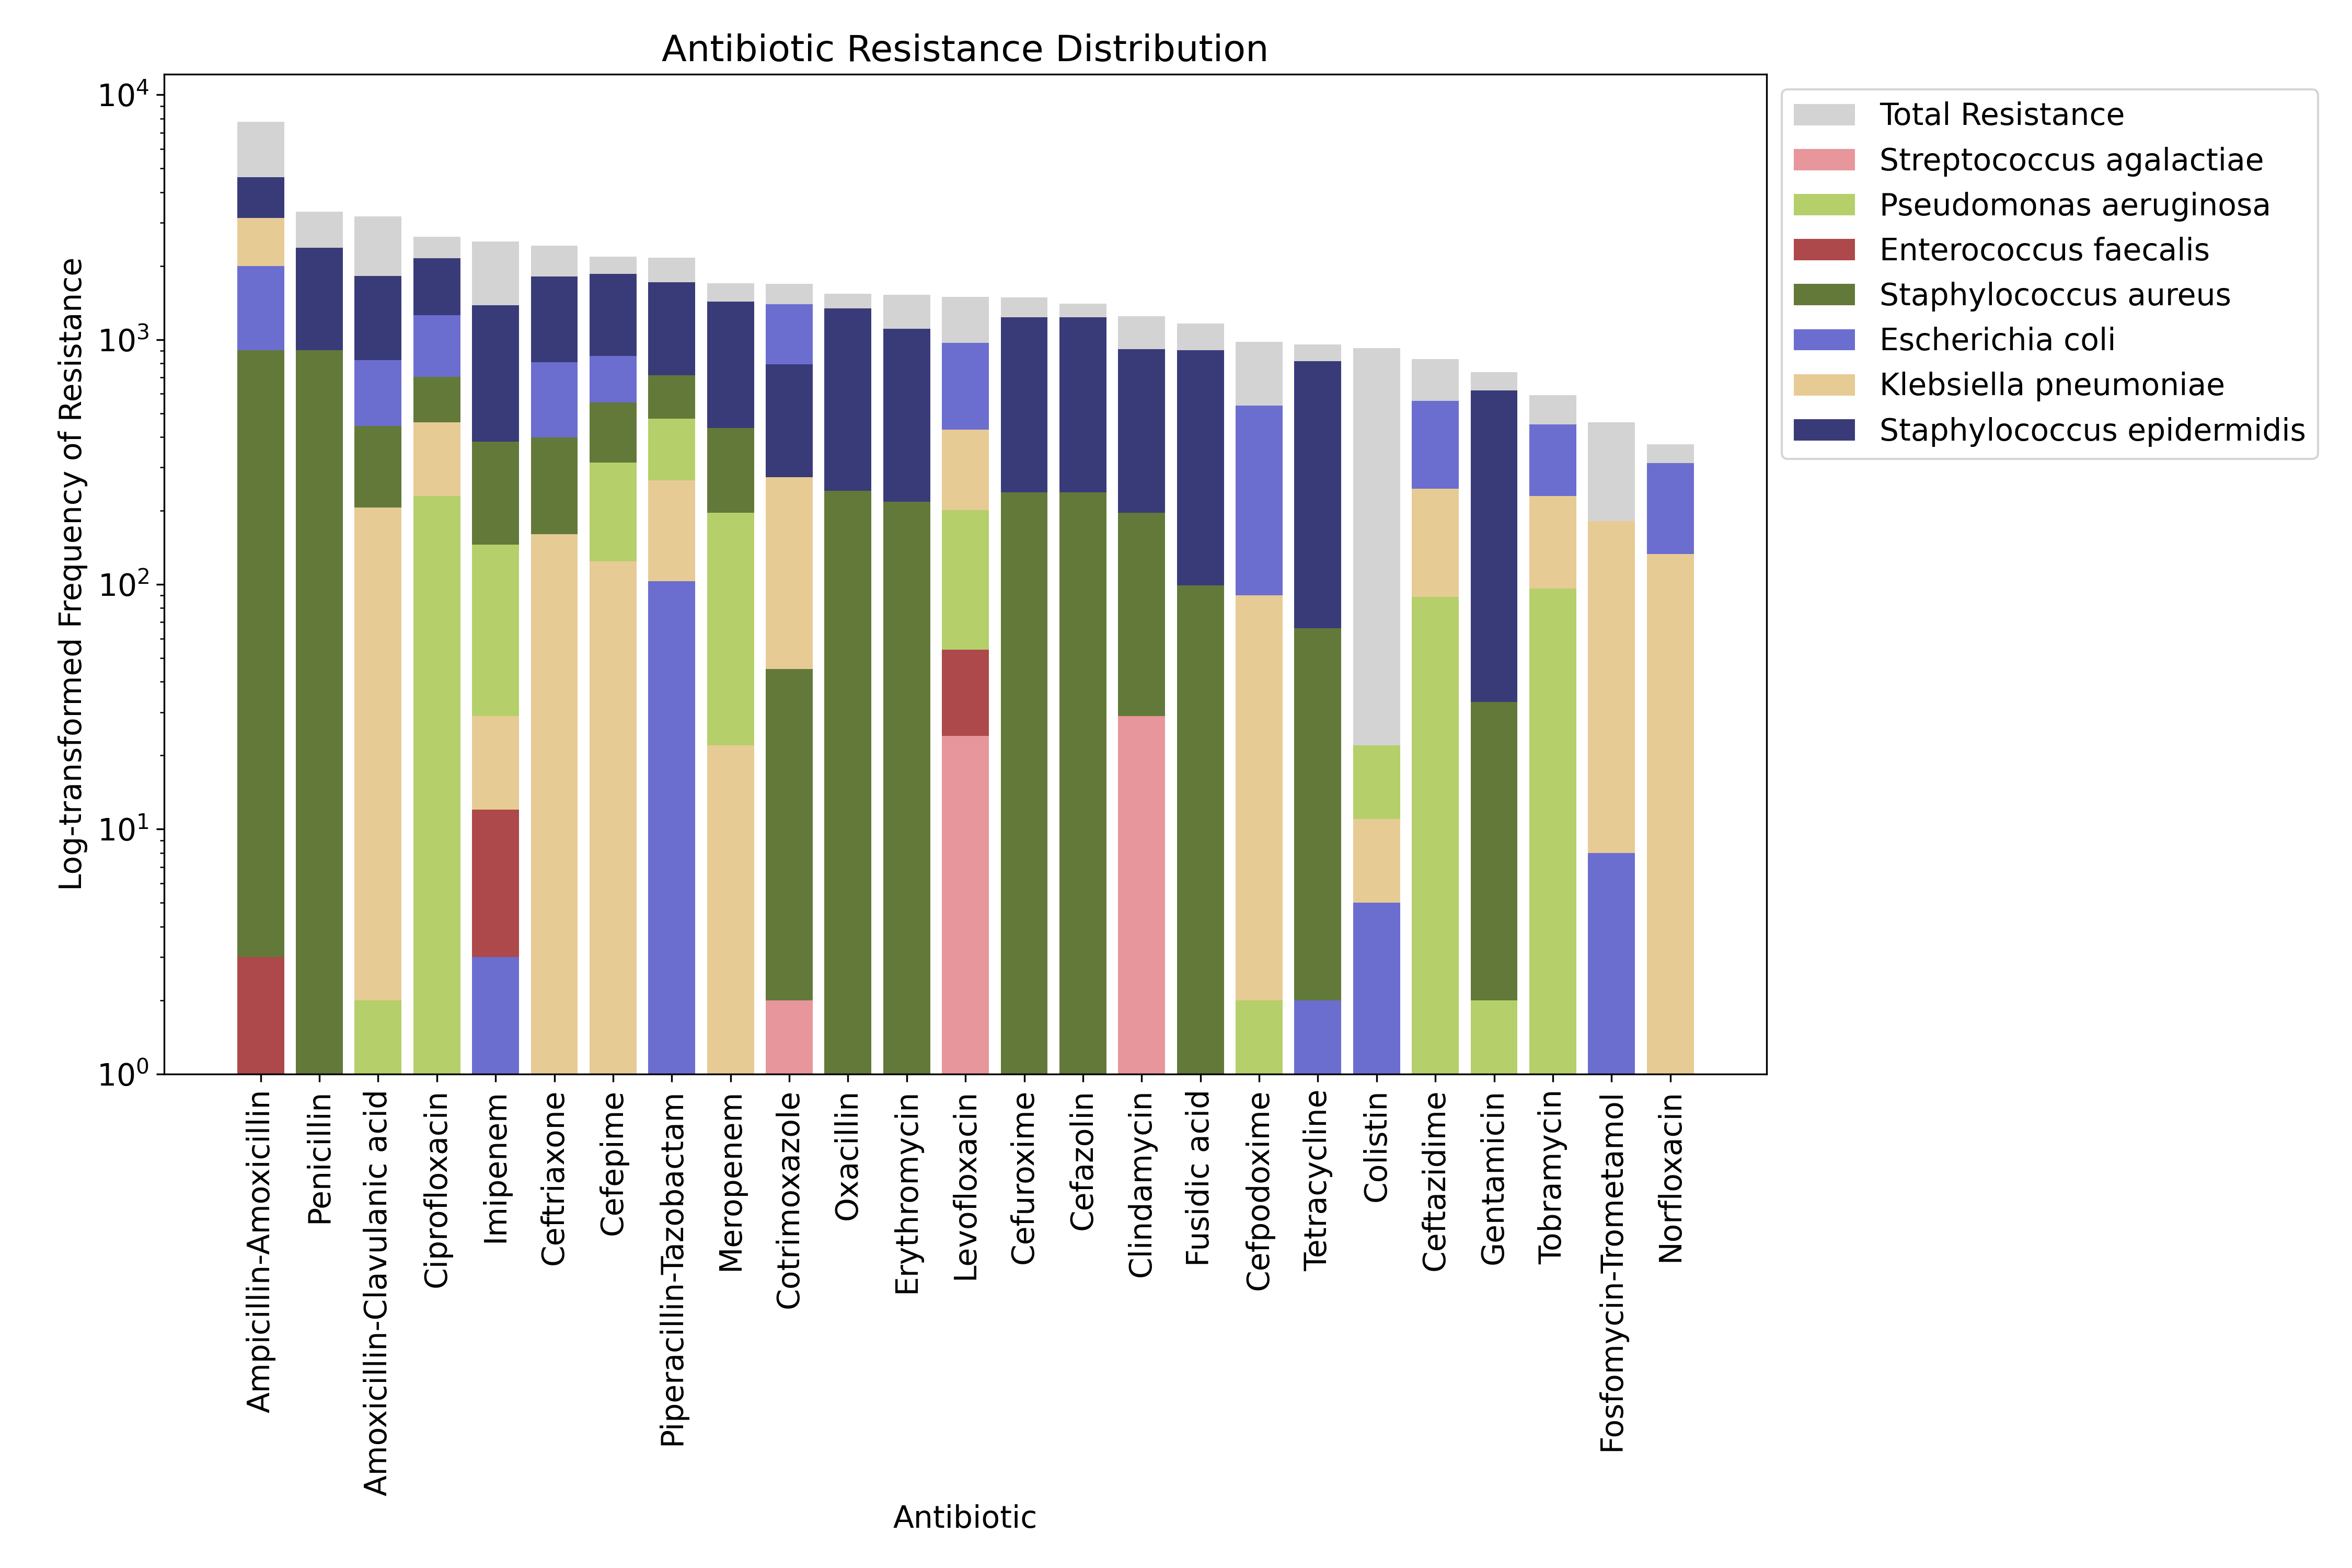
\includegraphics[width=0.95\textwidth]{img/antibiotic_resistance_distribution_filtered_2017.png}
	\caption{Antibiotic resistance distribution for the year 2017. The stacked bar plot shows the log-transformed frequency of resistance for the top 25 antibiotics. Each bar is divided by species, with colors representing different species. The total resistance count for each antibiotic is shown in gray, with contributions from individual species stacked below. Within each bar, species are sorted by their frequency of resistance, with species contributing fewer samples placed lower in the bar. The plot highlights the predominant species contributing to antibiotic resistance.}
	\label{fig:antibiotic_resistance_distribution}
\end{figure}

The data reveal that resistance is predominantly observed in a few species, with notable contributions from \textit{P. aeruginosa} (light green), \textit{S. aureus} (dark green), \textit{S. agalactiae} (pink), \textit{K. pneumoniae} (light brown), \textit{E. coli} (light blue), and \textit{S. epidermidis} (dark blue). These species frequently appear across multiple antibiotics.

The antibiotics with the highest frequency of resistance are Ampicillin-Amoxicillin, Penicillin, and Amoxicillin-Clavulanic acid. The resistance is primarily driven by \textit{S. epidermidis}, \textit{E. coli}, and \textit{S. aureus}. There is a noticeable variation in the species composition of resistance for different antibiotics.

\subsubsection*{Ridge Model Classification}
Figure \ref{fig:ROC_ridge} shows the ROC curves for the Ridge model. The top plot displays the ROC curves for the first 15 classes of antibiotics, with AUC values ranging from 0.78 to 0.87. Antibiotics such as Oxacillin and Cefazolin achieved the highest AUC values of 0.87, while Ciprofloxacin, Cotrimoxazole, and Levofloxacin had the lowest AUC values of 0.78. The bottom plot includes the ROC curves for the remaining 12 classes of antibiotics, where the AUC values range from 0.78 to 0.95. Colistin exhibited the highest AUC value, whereas Ceftriaxone and Piperacillin-Tazobactam had the lowest AUC values of 0.78. Overall, the Ridge model demonstrated a mean AUC value of 0.83 across the 27 antibiotics.

\begin{figure}[h]
	\centering
	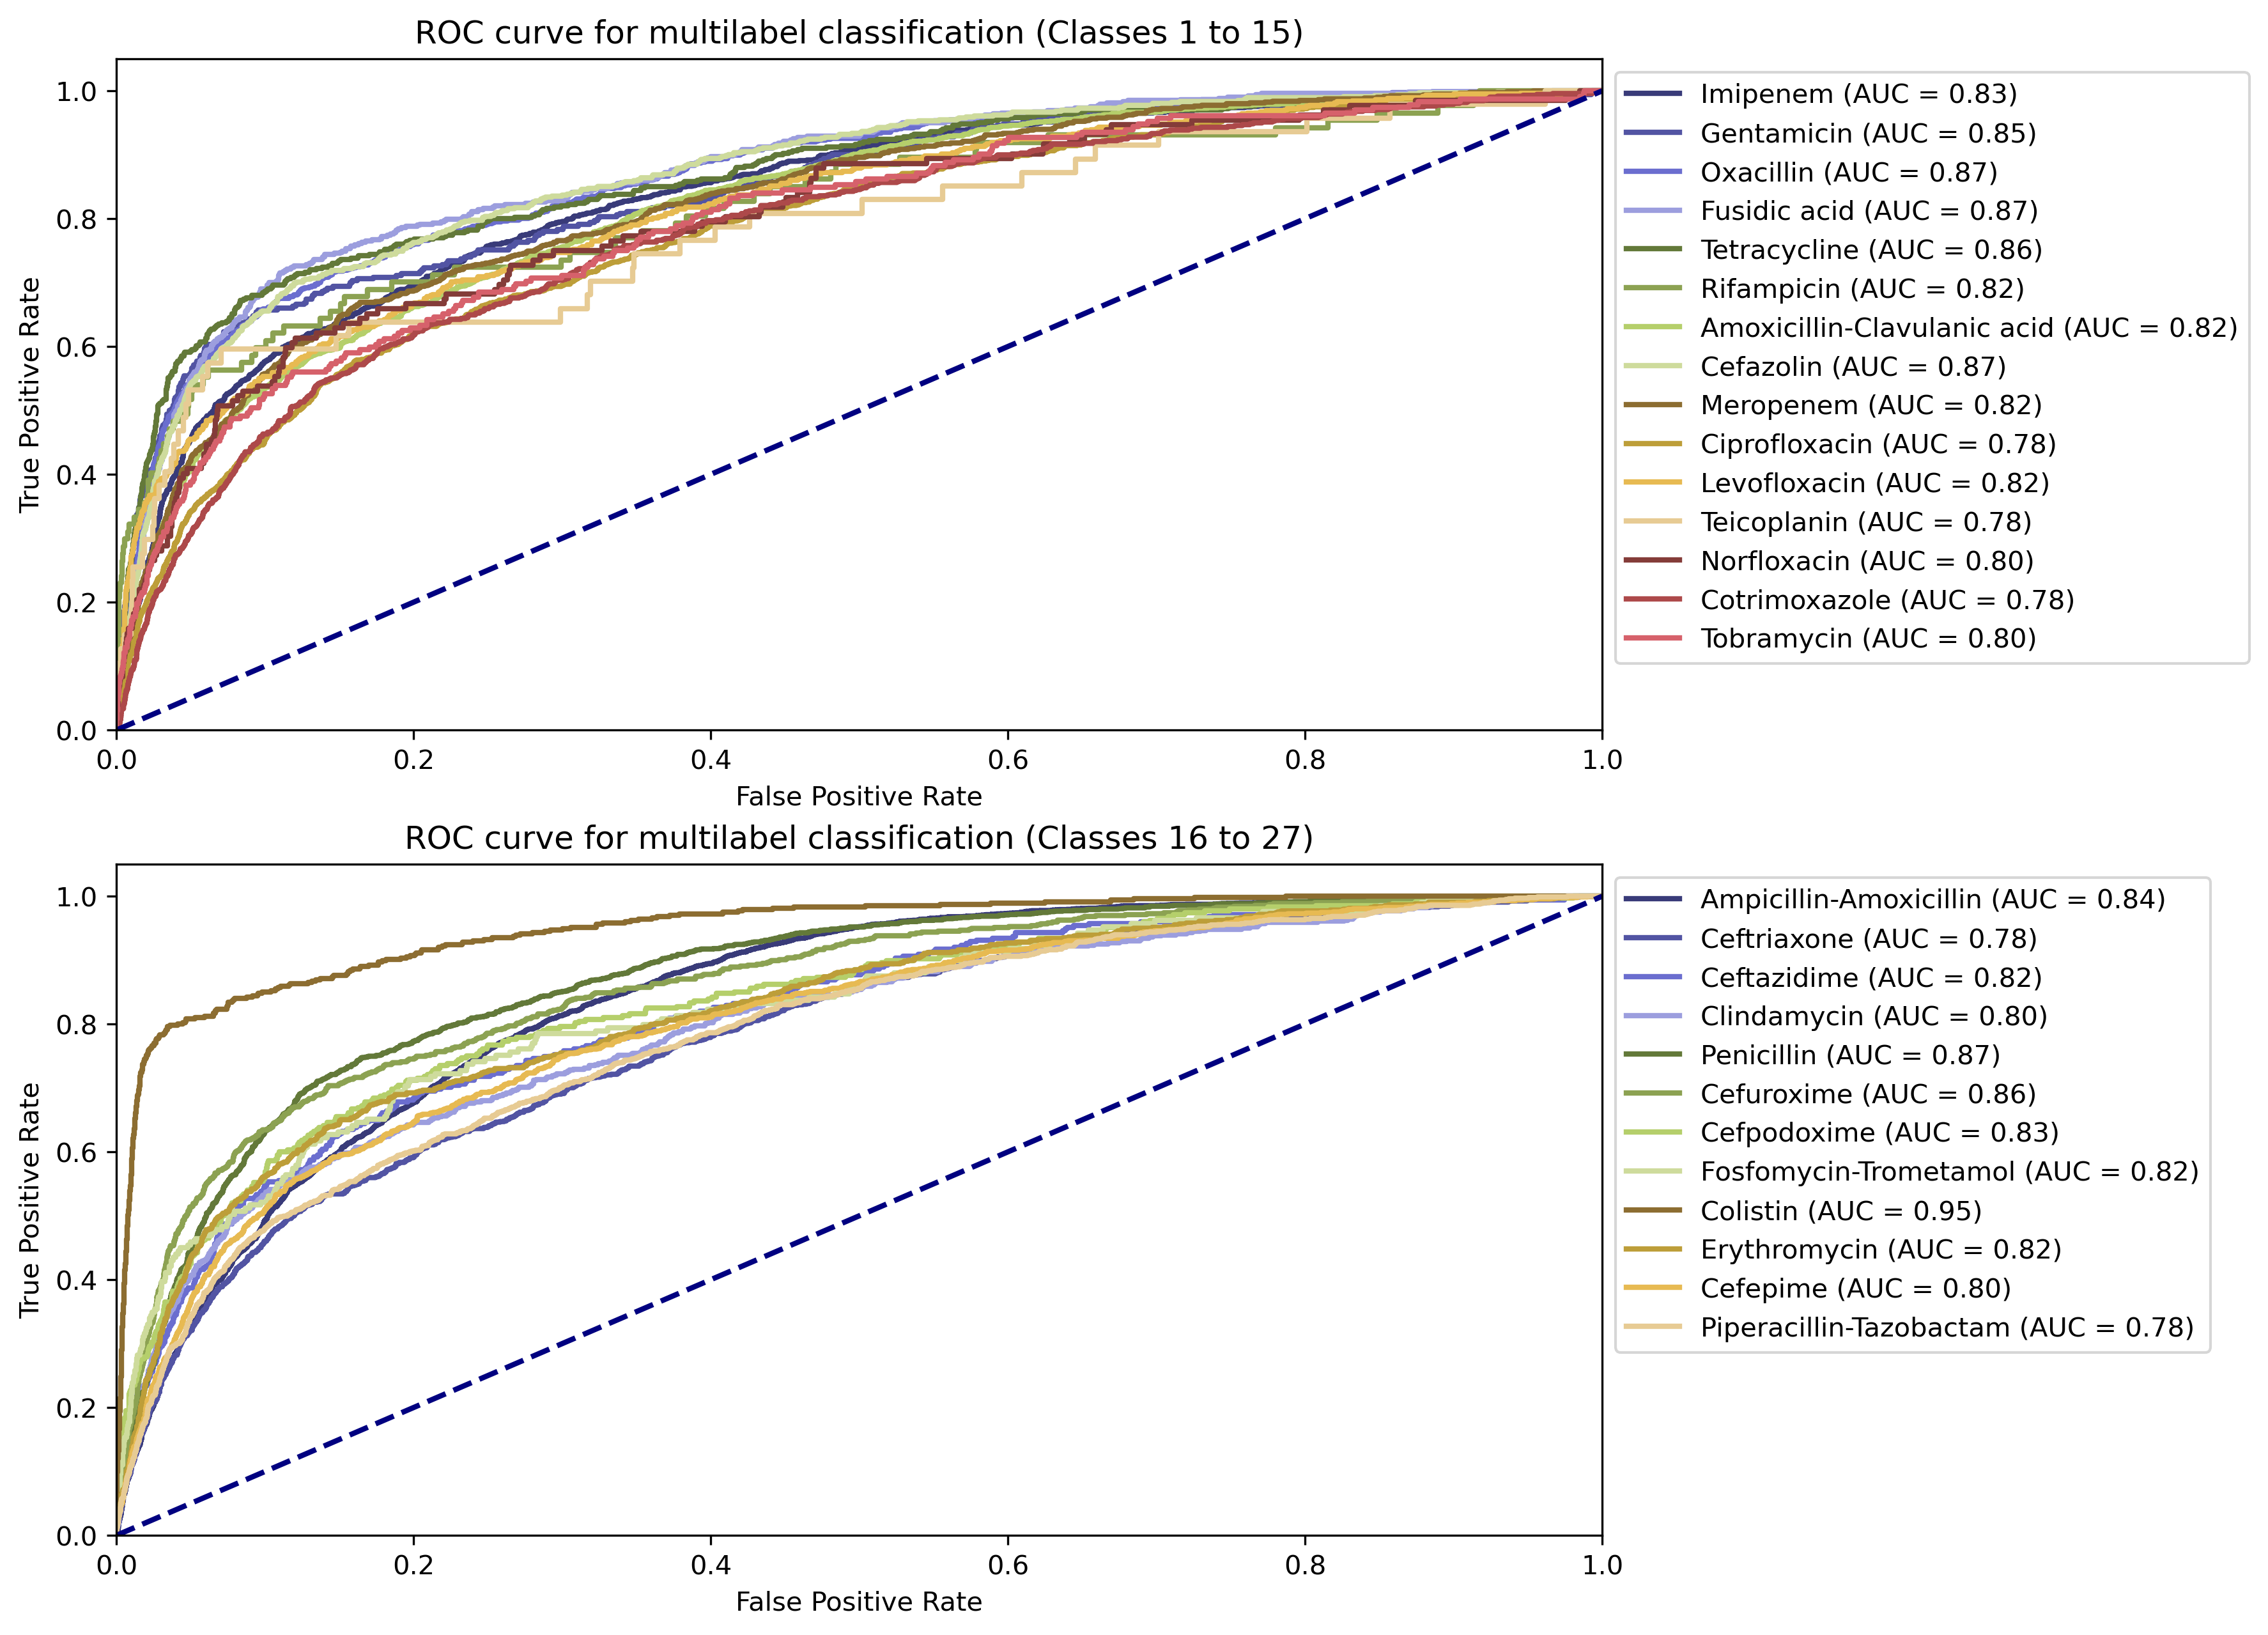
\includegraphics[width=0.9\textwidth]{img/ROC_curves_ridge.png}
	\caption{Receiver Operating Charateristic (ROC) curves for a Ridge model trained on the entire DRIAMS-A dataset (years 2015 to 2018 concatenated).The top plot displays the ROC curves for the first 15 antibiotics, with AUC values ranging from 0.78 to 0.87. The bottom plot shows the ROC curves for the remaining 12 antibiotics, with AUC values ranging from 0.78 to 0.95. The ROC curves illustrate the model's performance in classifying antibiotic resistance, with most antibiotics achieving AUC values above 0.8.}
	\label{fig:ROC_ridge}
\end{figure}

\subsubsection*{Random Forest Model Classification}
The ROC curves for the random forest model are presented in Figure \ref{fig:ROC_rf}. The top plot shows the ROC curves for the first 15 antibiotics, with AUC values ranging from 0.86 to 0.93. Tetracycline achieved the highest AUC value at 0.93, followed by Fusidic acid, Oxacillin, and Cefazolin with AUC values of 0.92. Ciprofloxacin and Cotrimoxazole had the lowest AUC values of 0.81 and 0.85, respectively. The bottom plot illustrates the ROC curves for the remaining 12 antibiotics, with AUC values ranging from 0.82 to 0.96. Colistin had the highest AUC value, while Ceftriaxone and Piperacillin-Tazobactam had the lowest AUC values of 0.82 and 0.85. The random forest model exhibited a mean AUC value of 0.89 across the 27 antibiotics.
\begin{figure}[h]
	\centering
	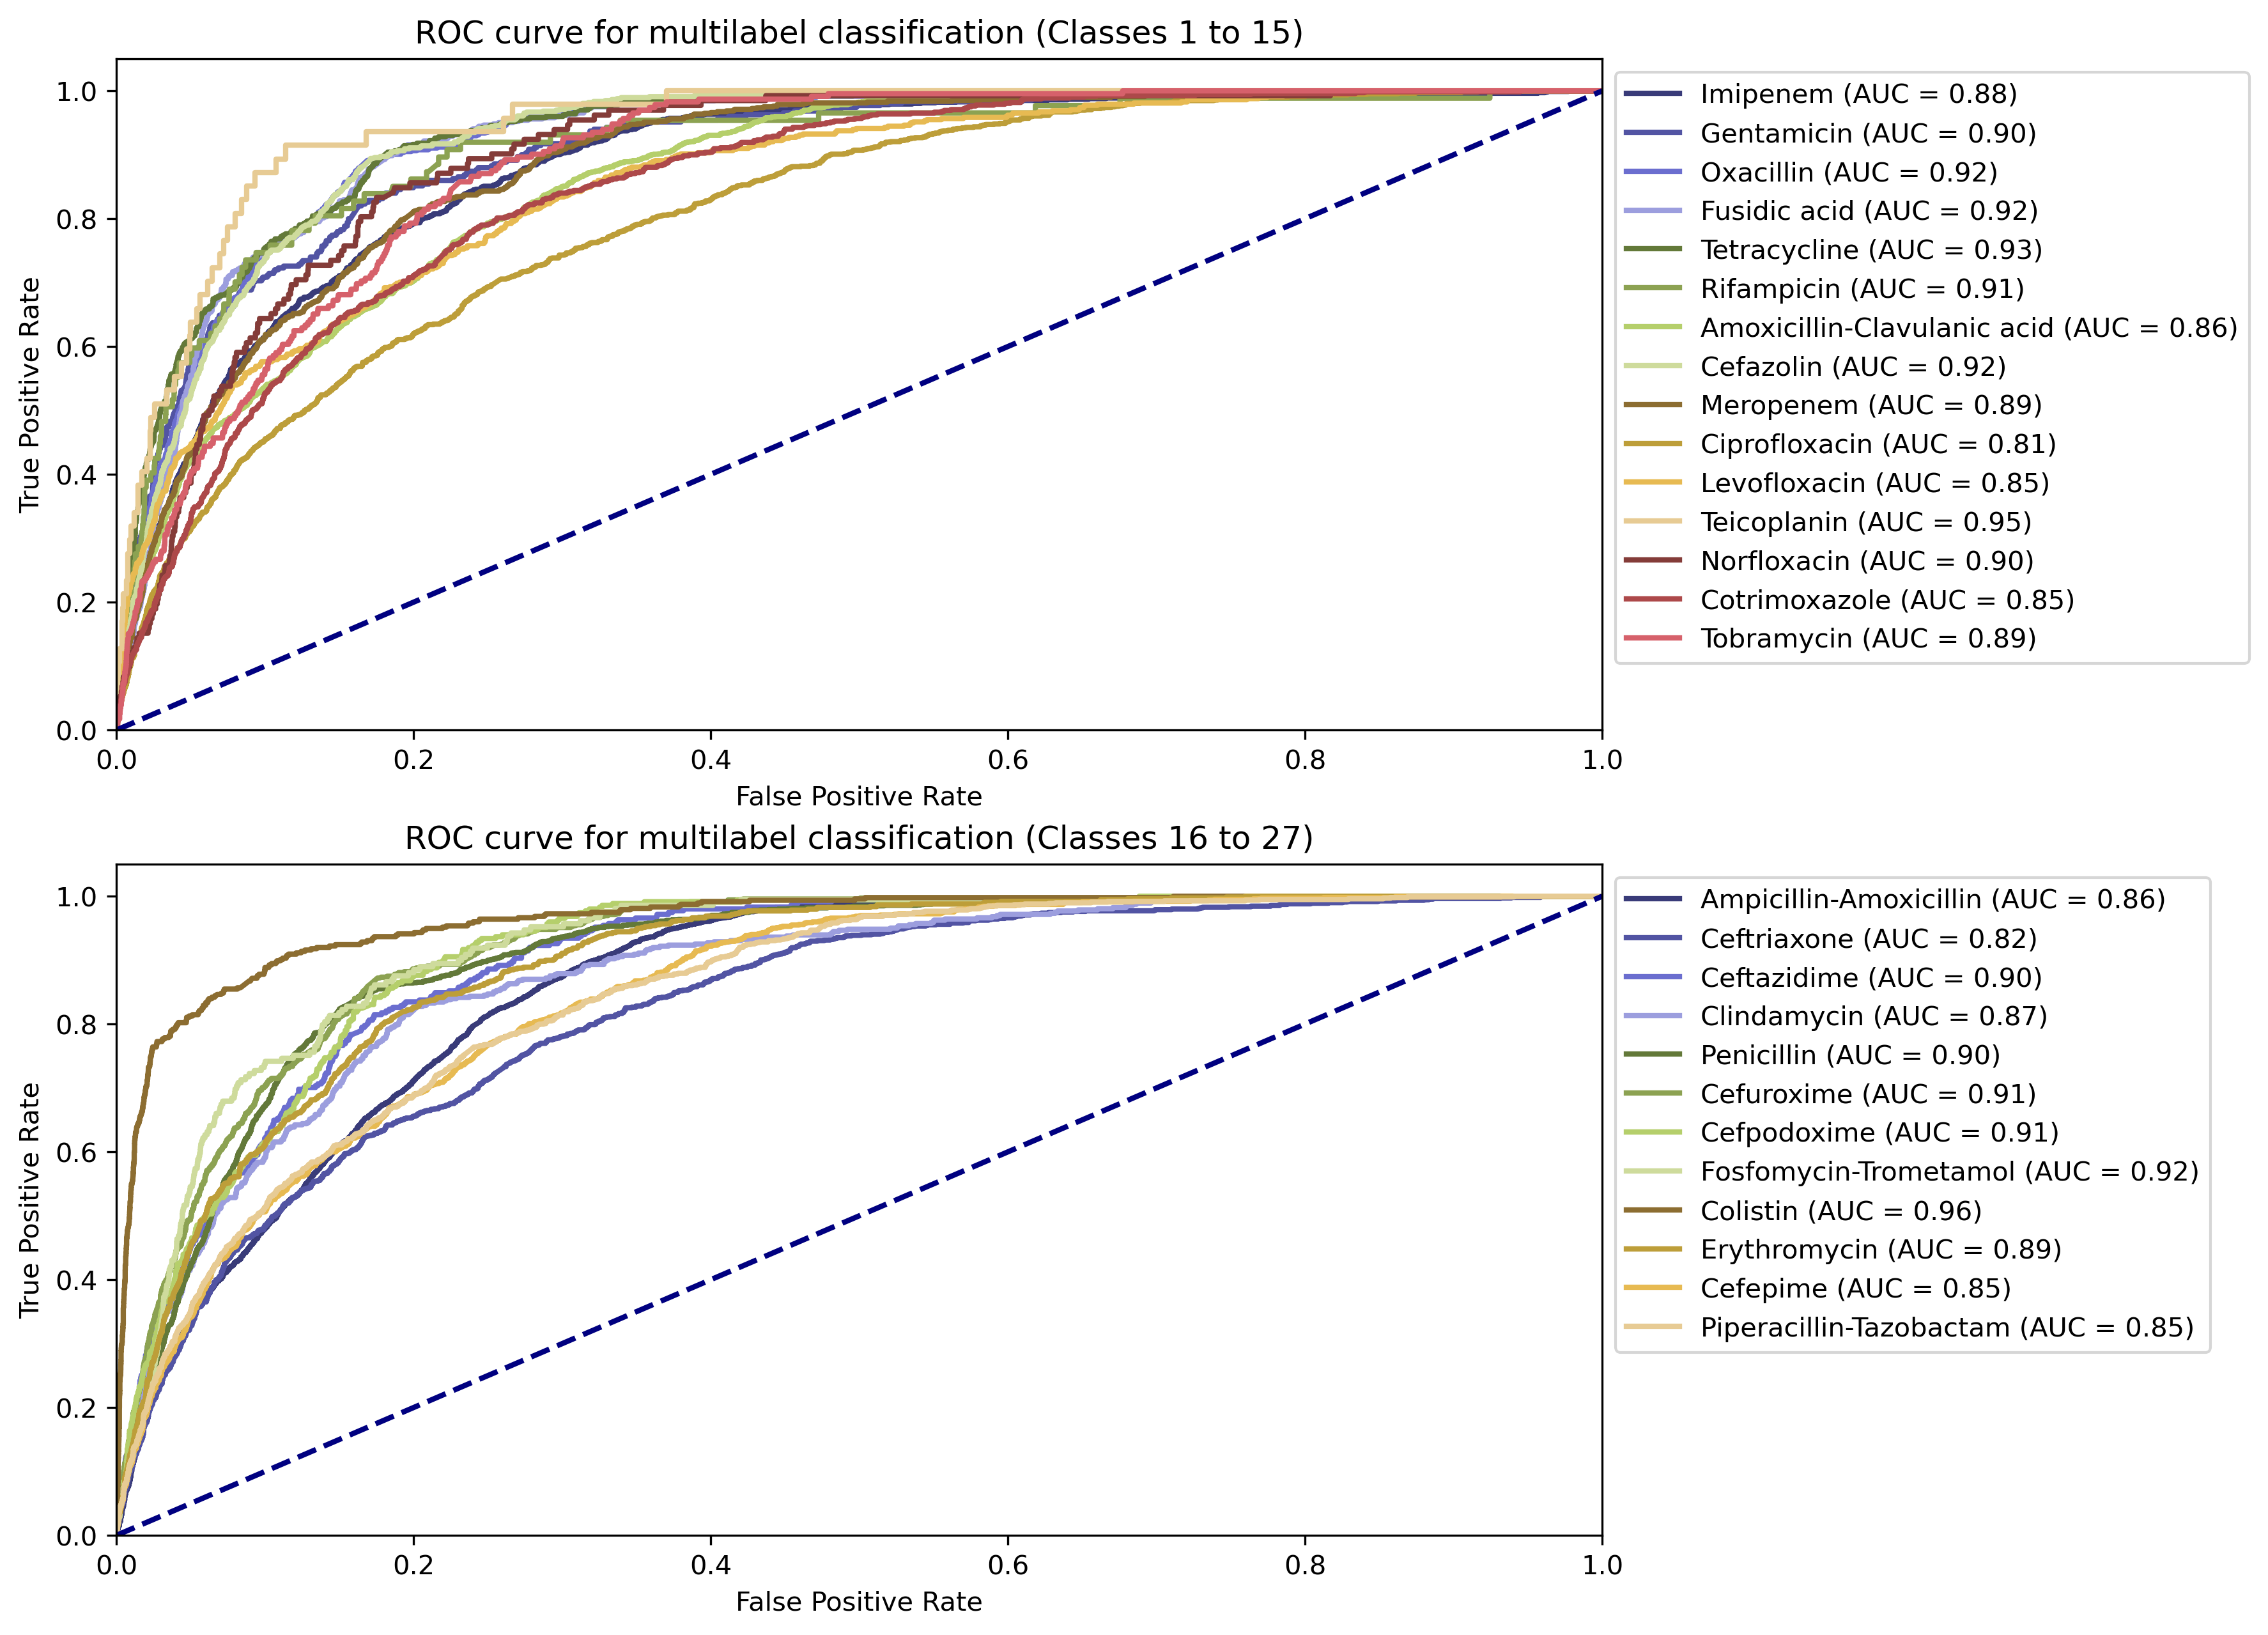
\includegraphics[width=0.9\textwidth]{img/ROC_curves_rf.png}
	\caption{Receiver Operating Characteristic (ROC) curves for a Random Forest model trained on the entire DRIAMS-A dataset (years 2015 to 2018 concatenated). The top plot displays the ROC curves for the first 15 antibiotics, with AUC values ranging from 0.86 to 0.93. The bottom plot shows the ROC curves for the remaining 12 antibiotics, with AUC values ranging from 0.82 to 0.96. The ROC curves illustrate the model's performance in classifying antibiotic resistance, with most antibiotics achieving AUC values above 0.8.}
	\label{fig:ROC_rf}
\end{figure}

\subsubsection*{Convolutional Neural Network Classification}
Figure \ref{fig:ROC_cnn} depicts the ROC curves for the CNN model. The top plot shows the ROC curves for the first 15 antibiotics, with AUC values ranging from 0.85 to 0.94. Oxacillin, Fusidic acid, Cefazolin, and Tetracycline achieved the highest AUC values of 0.94 each. Ciprofloxacin and Cotrimoxazole had the lowest AUC values of 0.85 and 0.86. The bottom plot presents the ROC curves for the remaining 12 antibiotics, with AUC values ranging from 0.85 to 0.98. Colistin had the highest AUC value, while Ceftriaxone had the lowest AUC value of 0.85. The CNN model had a mean AUC value of 0.90 across the 27 antibiotics.

\begin{figure}[h!]
	\centering
	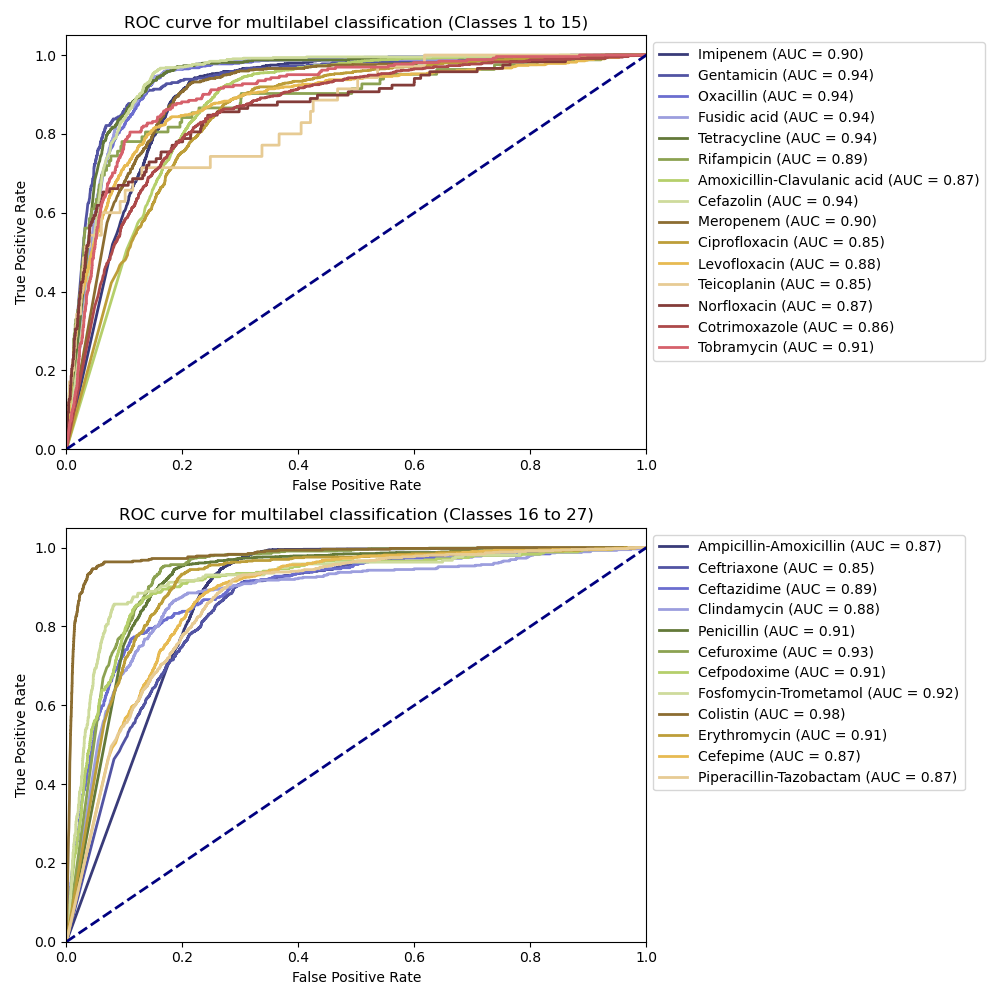
\includegraphics[width=0.9\textwidth]{img/FBeta_SiLU_ROC_curve.png}
	\caption{Receiver Operating Characteristic (ROC) curves for a Convolutional Neural Network (CNN) model trained on the entire DRIAMS-A dataset (years 2015 to 2018 concatenated). The top plot displays the ROC curves for the first 15 antibiotics, with AUC values ranging from 0.85 to 0.94. The bottom plot shows the ROC curves for the remaining 12 antibiotics, with AUC values ranging from 0.85 to 0.98. The ROC curves illustrate the model's performance in classifying antibiotic resistance, with most antibiotics achieving AUC values above 0.85.}
	\label{fig:ROC_cnn}
\end{figure}

\subsection*{Feature Extraction}
Feature importance values were extracted from the CNN model for 24 different types of antibiotics using two methods: Shapley Value Sampling and GradCAM. Below is shown the results of both methods for Tobramycin resistance.

\subsubsection*{Shapley Value Sampling}
The Shapley value sampling method's results are illustrated in the Figure \ref{fig:feature_shapley}. The top plot shows the Shapley value feature importance across the m/z ratio mass spectrum. The bottom plot overlays these Shapley values on the original mass spectrum. Positive Shapley values indicate features that positively contribute to the prediction of Tobramycin resistance, while negative values indicate features that negatively contribute. The distribution of Shapley values appears relatively sparse, with significant positive and negative peaks around specific m/z values, suggesting certain regions of the mass spectrum are critical for predicting resistance.

\subsubsection*{GradCAM}
The GradCAM method's results are shown in Figure \ref{fig:feature_gradcam}. Similarly, the top plot shows the GradCAM feature importance across the mass spectrum, while the bottom plot overlays these values on the original mass spectrum. GradCAM values highlight regions of the spectrum that significantly influence the CNN's prediction. The feature importance appears sparser across the spectrum compared to the Shapley values, but also highlights specific peaks that are crucial for the model's decision-making.

\begin{figure}[h]
	\centering
	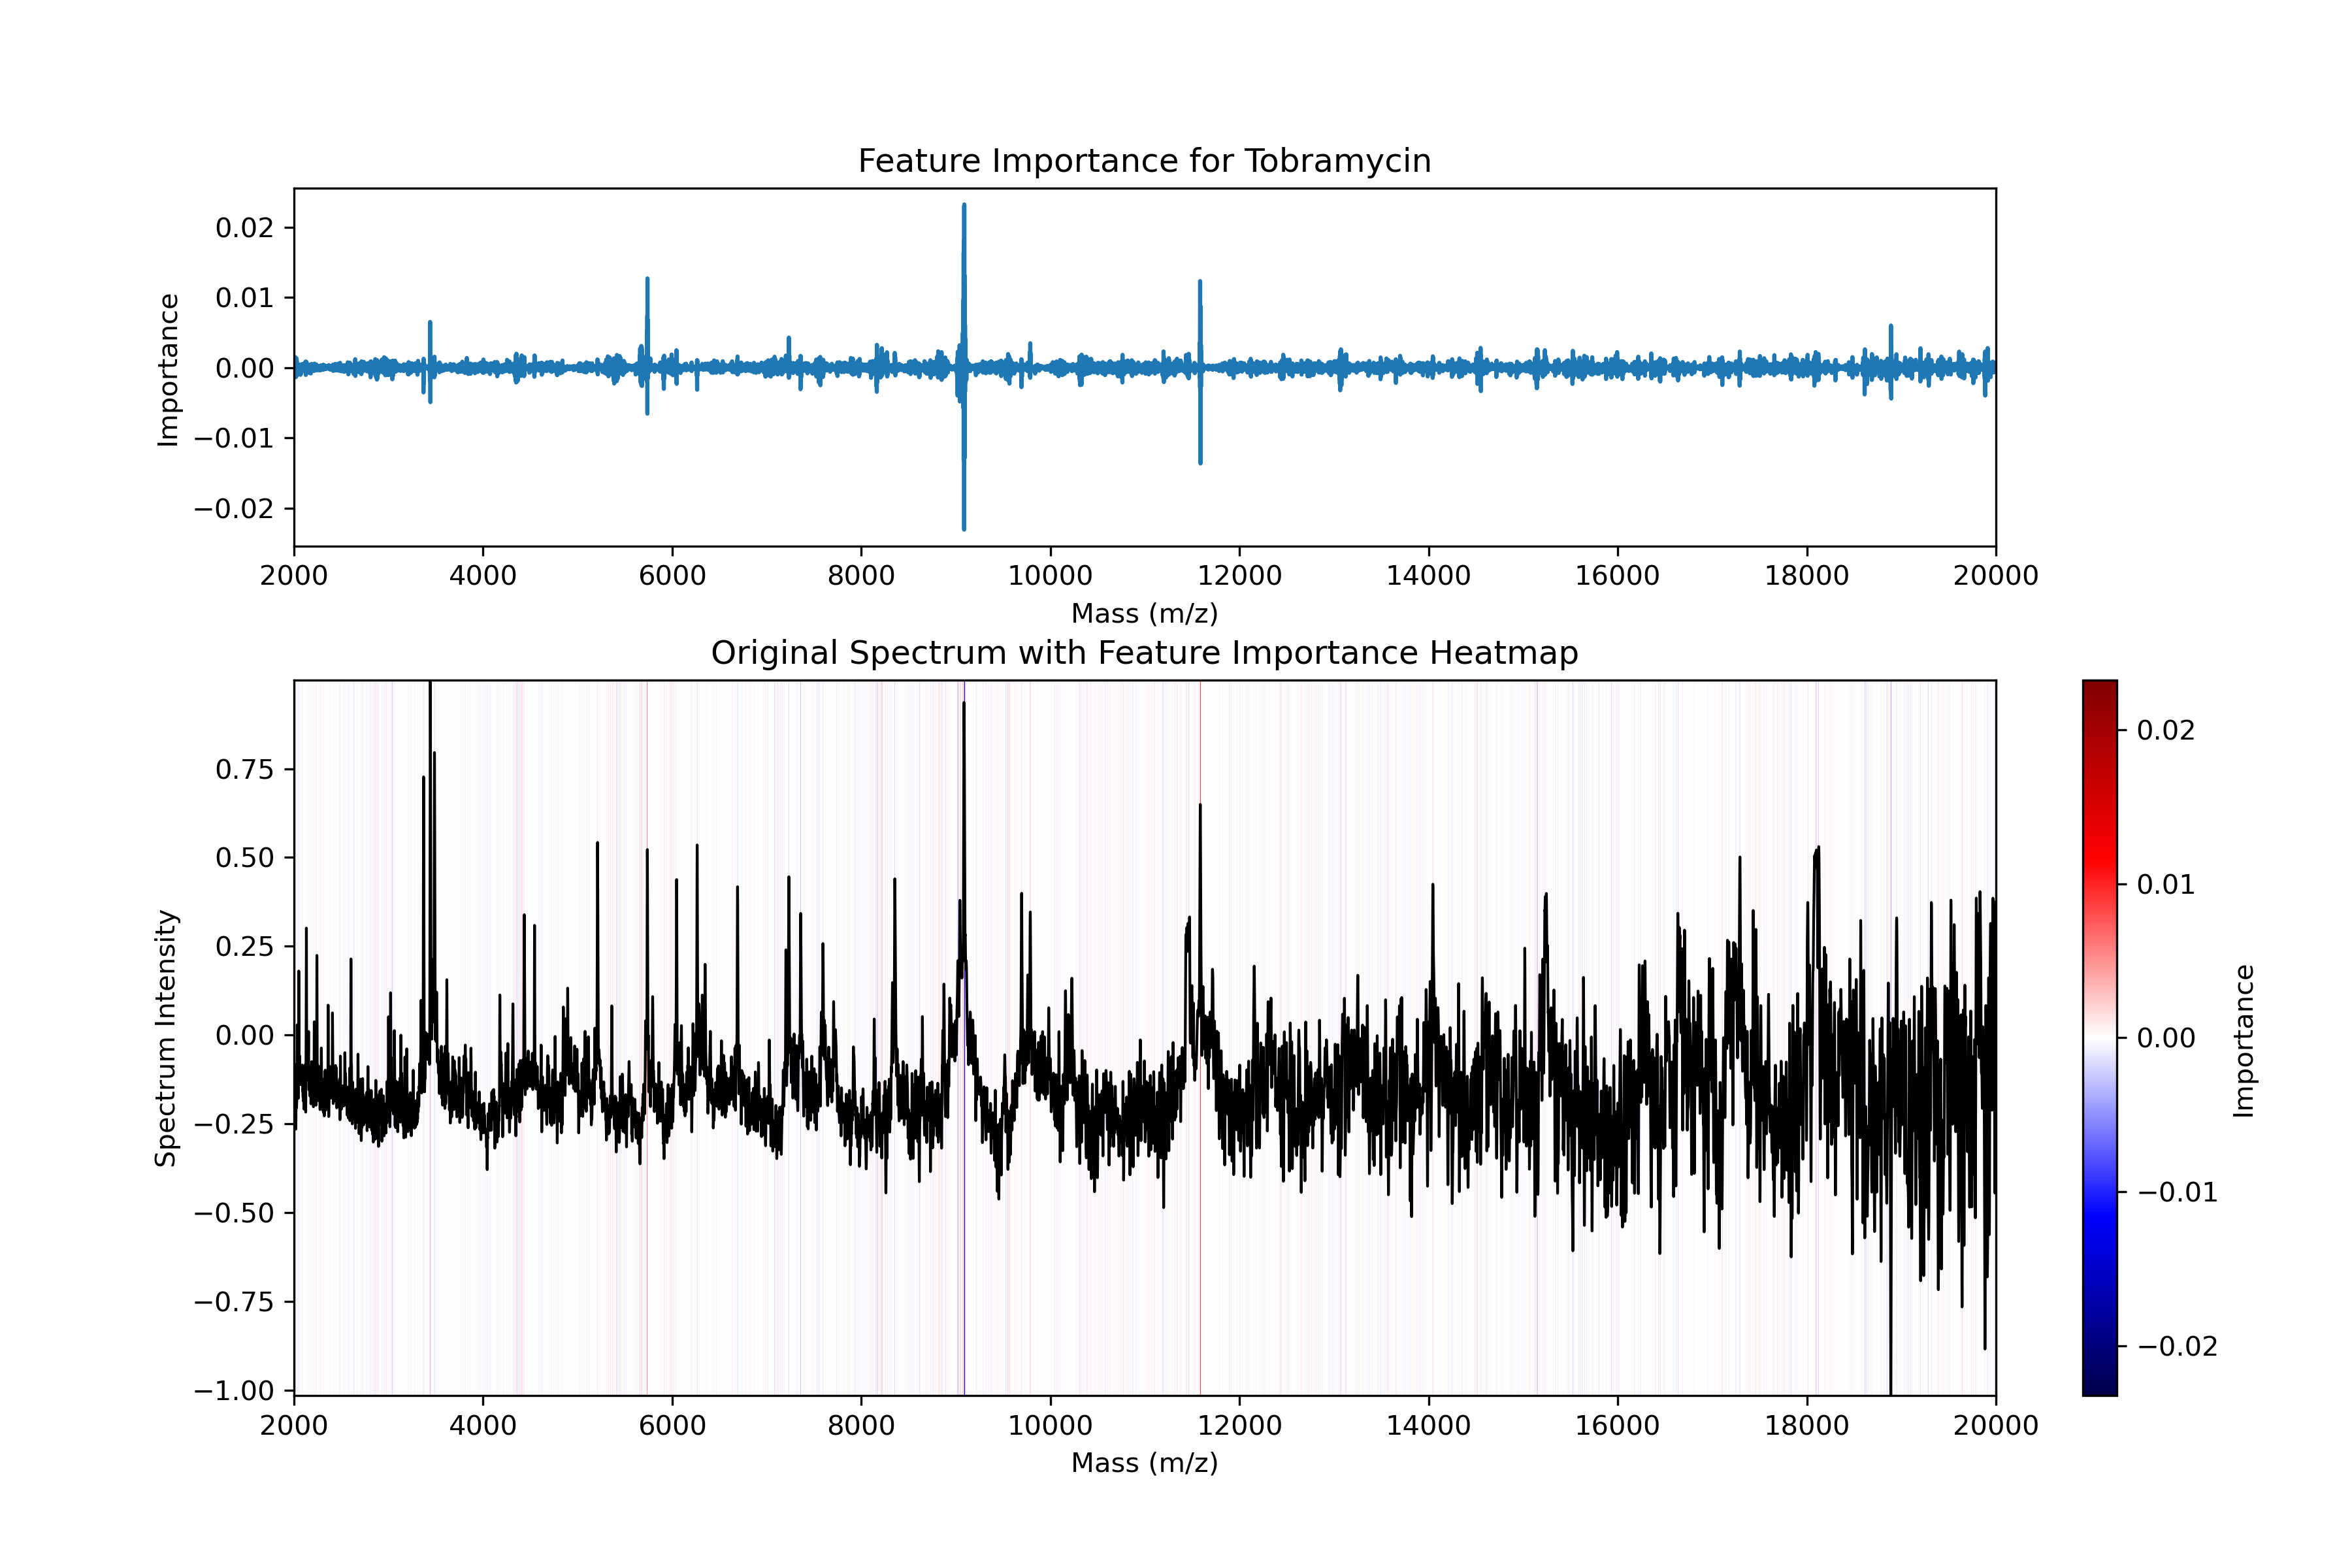
\includegraphics[width=0.9\textwidth]{img/Tobramycin_shapley.png}
	\caption{Feature importance values derived using Shapley value sampling for a CNN model predicting Tobramycin resistance. The top plot shows Shapley values across the mass spectrum, while the bottom plot overlays these values on the original MALDI-TOF mass spectrum. Positive and negative Shapley values indicate features that contribute positively and negatively to the prediction, respectively.}
	\label{fig:feature_shapley}
\end{figure}
\begin{figure}[h]
	\centering
	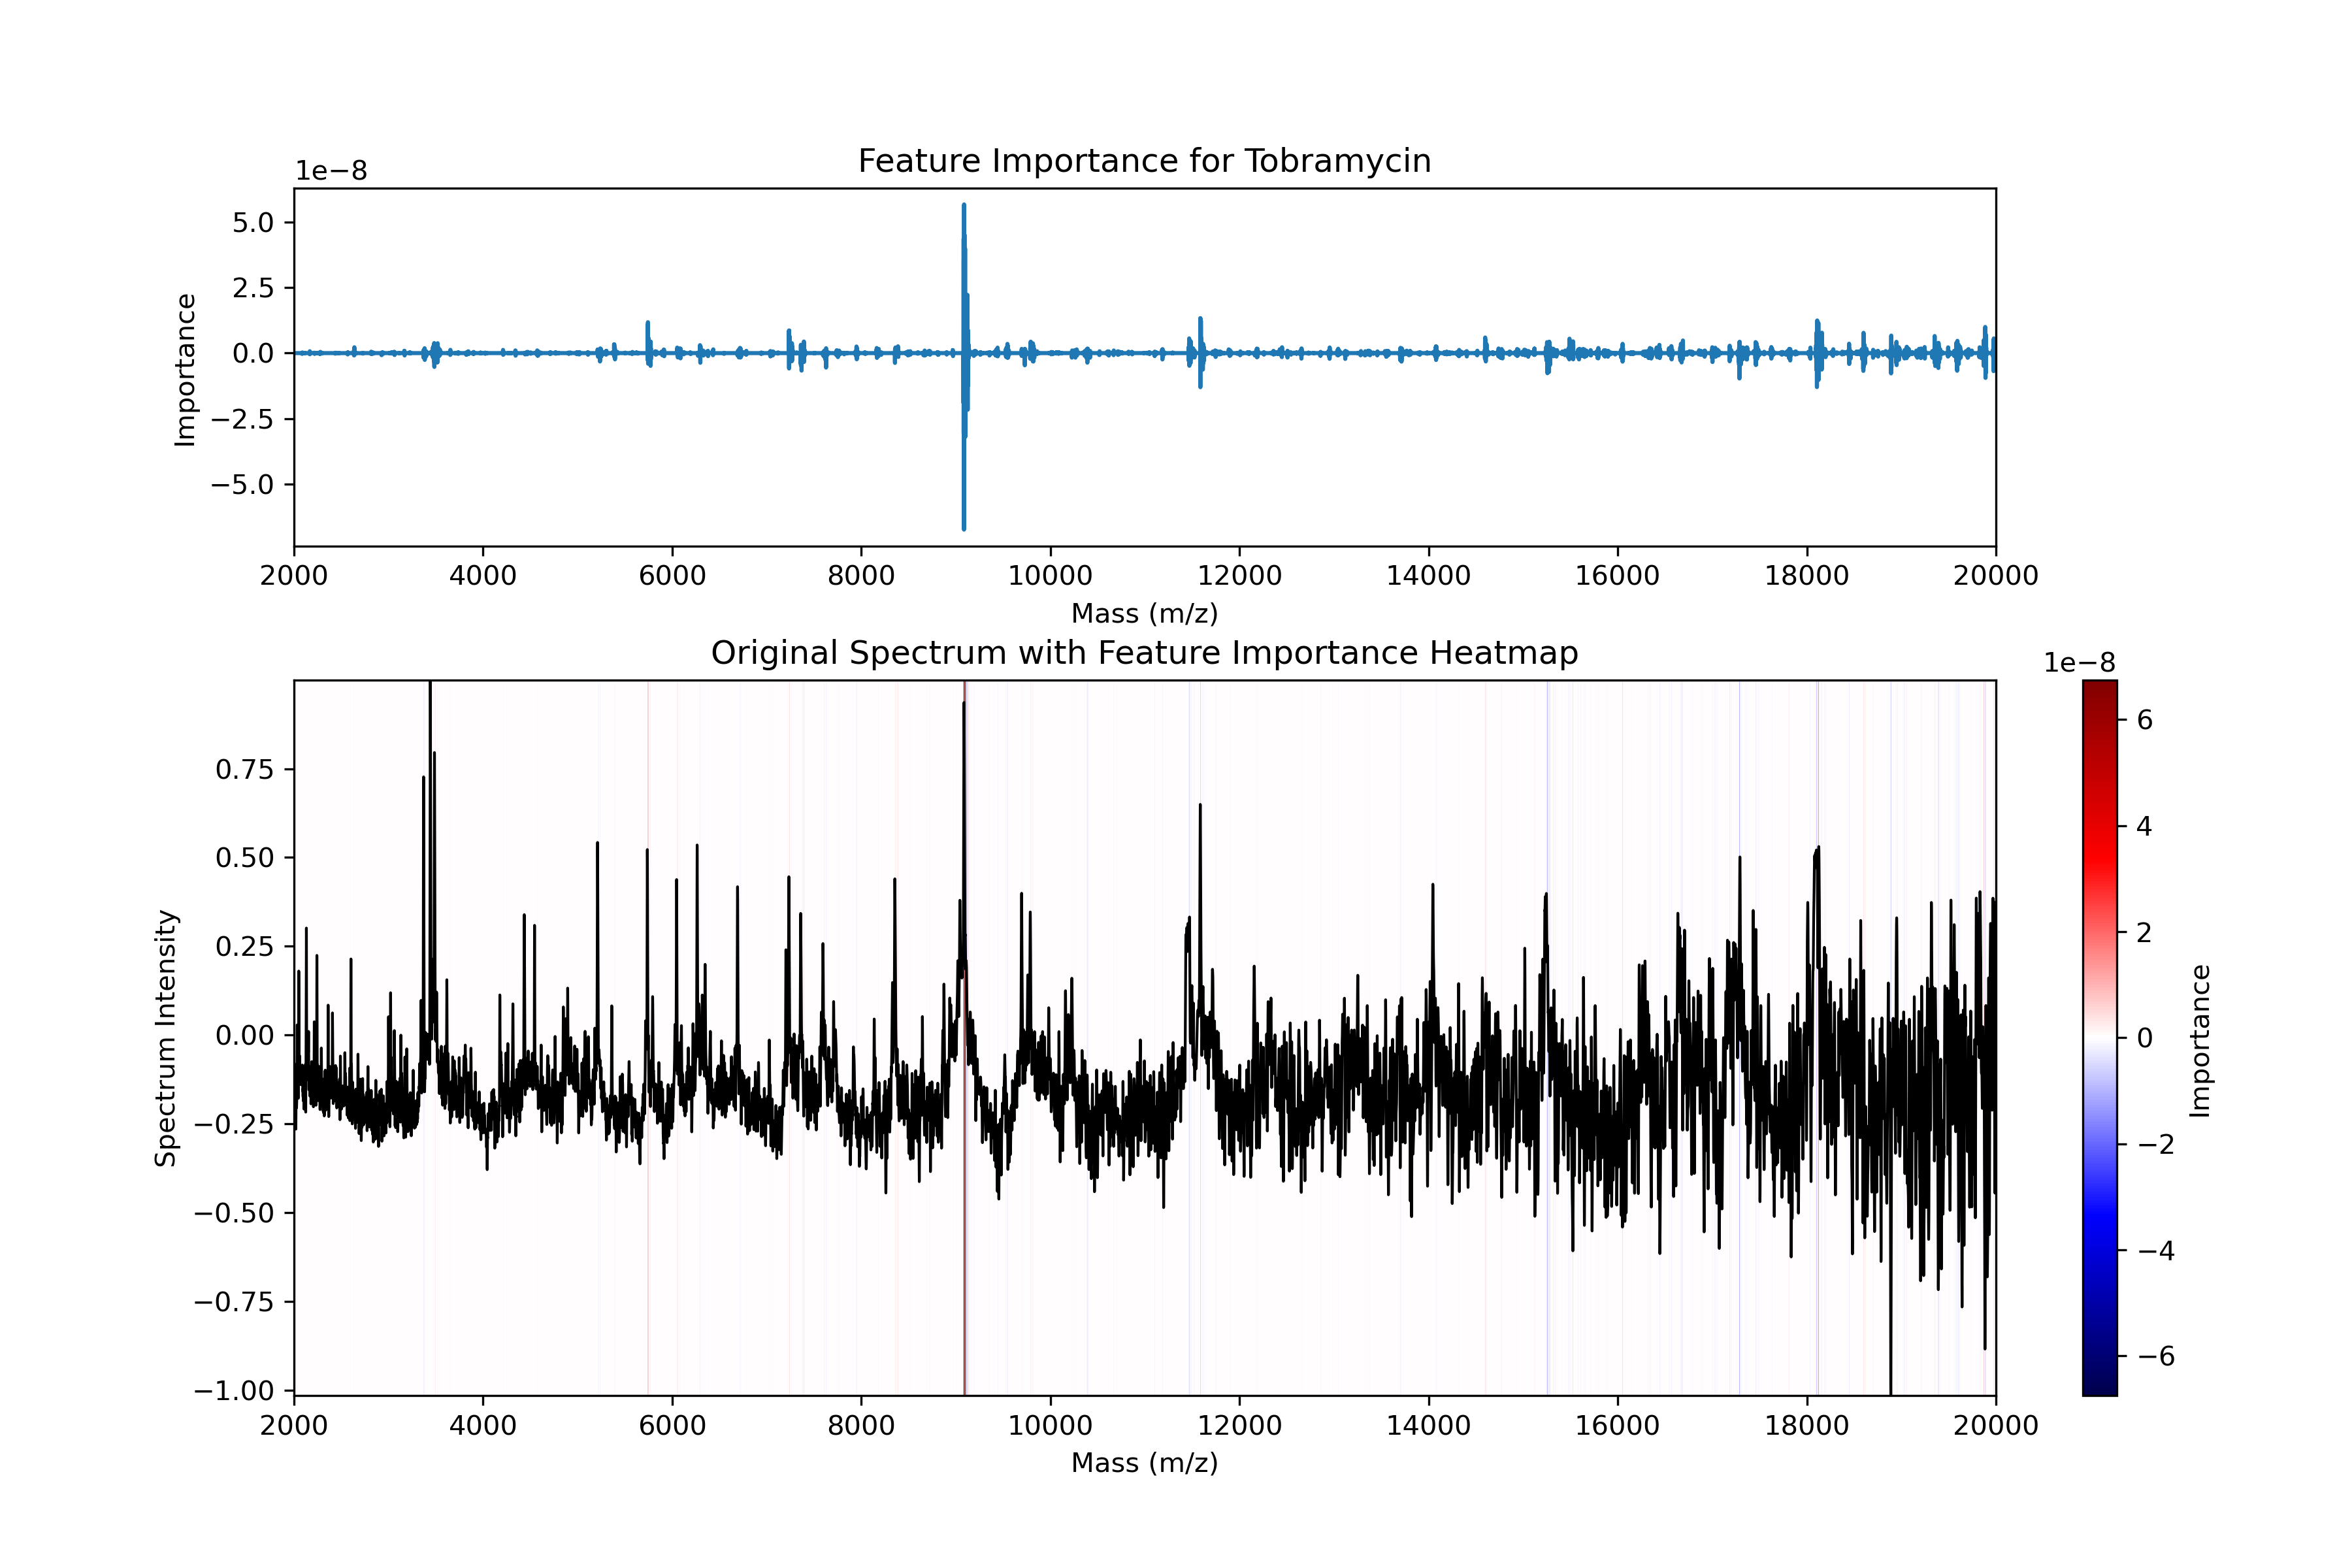
\includegraphics[width=0.9\textwidth]{img/Tobramycin_gradcam.png}
	\caption{Feature importance values derived using GradCAM for a CNN model predicting Tobramycin resistance. The top plot shows GradCAM values across the mass spectrum, while the bottom plot overlays these values on the original MALDI-TOF mass spectrum. GradCAM highlights regions of the spectrum that significantly influence the CNN's prediction.}
	\label{fig:feature_gradcam}
\end{figure}

\clearpage

\section*{Discussion}
\subsection*{Species Classification}
\subsubsection*{Distribution of Species}
The distribution of the top 10 species from 2015 to 2018 reveals significant insight into the composition and prevalence of various bacterial species over these years. As depicted in Figure \ref{fig:species_distribution}, there is a notable consistency in the top species across the years, with some fluctuations in their relative proportions.

\textit{S. epidermidis} and \textit{E. coli} are consistently among the most prevalent species each year. This align with known data on hospital-acquired infections and common bacterial pathogens in clinical settings \cite{ottoStaphylococcusEpidermidisAccidental2009,russoMedicalEconomicImpact2003}. Over the four years, the top 10 species collectively account for an increasing proportion of the total species identified, ranging from 38.7\% in 2015 to 45.9\% in 2018. This increase may reflect a greater focus or higher detection rates of these species in clinical samples.

\subsubsection*{Dimensionality Reduction Methods}
Both PCA (Figure \ref{fig:species_pca}) UMAP (Figure \ref{fig:species_umap}) were applied to the 2017 dataset, which contains the largest number of data points. Similar patterns of segregation are observed in the other large datasets from 2016 and 2018, while some differences are noted in the 2015 dataset, likely due to its smaller sample size (see supplementary 4-9).

UMAP demonstrates a clearer separation of species compared to PCA. Distinct clusters are more apparent in the UMAP plot, while some singular data points appear between clusters or in unmatched clusters. The exact reason for this occurrence is uncertain, but it may be attributed to noise or potential mislabeling of data points.

Overall, these dimensionality reduction techniques provide valuable insights into the structure of the dataset, with UMAP offering a more effective visualization of species segregation.

\subsubsection*{Machine Learning Model Comparison}
Ridge exhibits moderate performance across all years, with mean test scores ranging approximately between 0.2 and 0.6. Although there is some variability in its performance, Ridge generally does not achieve the highest accuracy among the models. This moderate performance can be attributed to the ability of Ridge to handle multicollinearity by penalizing large coefficients, thereby improving generalization but not excelling in prediction accuracy for this dataset. The underperformance of Ridge, along with elastic net, suggests that linear models are insufficient for capturing the complex interactions necessary to accurately classify species within this dataset. The nature of the data likely requires models capable of capturing non-linear relationships and interactions between features.

In contrast, random forest demonstrates relatively high and consistent performance, with mean test scores often exceeding 0.8. The ensemble nature of random forest, which aggregates the predictions of multiple decision trees, contributes to its robustness and ability to handle complex interactions within the data. This model’s effectiveness in capturing non-linear relationships and reducing overfitting makes it a reliable choice for species classification.

Elastic net shows poor performance compared to the other models, with mean test scores mostly below 0.2. This model appears to struggle with species classification, likely due to its simultaneous application of L1 and L2 penalties, which can lead to overshrinking of coefficients and insufficient complexity to capture the data patterns. The underperformance of elastic net highlights its limitations in scenarios requiring high-dimensional feature interactions and underscores the necessity for more complex models that can capture the nuances in the data.

The SVM model achieves the highest mean test scores, often close to 1.0 for the years 2016 through 2018. SVM also shows high performance for 2015 but with slightly more variability. The strength of SVM lies in its ability to find the optimal hyperplane that separates classes with maximum margin, which is particularly beneficial in high-dimensional spaces. 

The findings from this comparison align with the results presented by Mortier et al. (2019) \cite{mortierBacterialSpeciesIdentification2021} in their benchmarking study of bacterial species identification using MALDI-TOF mass spectrometry and machine learning techniques. Mortier et al. also observed that SVM outperforms other models, including random forest, in species identification tasks. The high accuracy of SVM in both studies underscores its robustness and effectiveness in handling complex biological data.

A relevant consideration in this analysis is the potential impact of data quality over the years. If the physical machinery used to record the data was not properly maintained or if it experienced wear due to regular usage, one might expect data drift over time. This drift could lead to inconsistencies, which would manifest as poorer performance in the aggregated category compared to individual years. However, the aggregated category does not perform worse than the individual years. This suggests that either the data quality has been consistently maintained across the years, or that the models used are robust enough to handle any minor variations in the data.

Overall, the SVM model emerges as the top performer in species prediction, followed by Random Forest, which also demonstrates high and consistent accuracy. Ridge Regression provides moderate performance, while Elastic Net consistently underperforms. These results emphasize the importance of model selection in bioinformatics applications and highlight the superior capabilities of SVM and Random Forest in species classification tasks. Integrating insights from Mortier et al. (2019) strengthens the evidence for the reliability of SVM and Random Forest in complex predictive tasks.

\subsection*{Antimicrobial Resistance}
\subsubsection*{Resistance Distribution}
The analysis of antibiotic resistance distribution across different species for the year 2017, as visualized in Figure \ref{fig:antibiotic_resistance_distribution}, highlights significant insights into the patterns of resistance. For a comprehensive understanding of these trends over the years, visualizations for the years 2015, 2016, and 2018 are included in the supplementary materials (Figures S10-S12). These figures illustrate similar resistance distributions for the top 25 antibiotics in each respective year.

In 2015, the resistance profile is similar to that observed in 2017, with \textit{S. epidermidis}, \textit{E. coli}, and \textit{S. aureus} being the primary contributors. This consistency suggests stable resistance patterns for these species across the years.

The 2016 data show a slight shift in the species contributing to resistance, with increased contributions from \textit{P. aeruginosa} and \textit{K. pneumoniae} for certain antibiotics. This shift might be attributed to changes in antibiotic usage, bacterial evolution, or differences in sample collection and analysis methods.

By 2018, the resistance trends largely mirror those observed in 2017, with continued dominance of \textit{S. aureus}, \textit{E. coli}, and \textit{S. epidermidis}. However, there is an increased presence of \textit{S. agalactiae} and \textit{P. aeruginosa} for some antibiotics, indicating ongoing shifts in resistance patterns.

These findings align with broader studies on antimicrobial resistance, which consistently identify \textit{S. aureus} and \textit{E. coli} as major contributors due to their prevalence and adaptability. Tacconelli et al. (2018) \cite{tacconelliDiscoveryResearchDevelopment2018} provide extensive evidence on the prevalence of resistance in these species, highlighting their significant role in the global burden of antimicrobial resistance.

\subsubsection*{Model Performance}
The performance of the Ridge and random forest models in classifying antibiotic resistance was evaluated using ROC curves (Figures \ref{fig:ROC_ridge} and \ref{fig:ROC_rf}). The preprocessing steps, particularly log-transformation, LOWESS smoothing, and rescaling, were crucial in stabilizing variance, normalizing the data, and enhancing signal clarity by reducing noise.

In contrast, Weis et al. (2022) \cite{weisDirectAntimicrobialResistance2022} used a different preprocessing approach. They binned the mass spectra with a bin size of 3 Da to handle measurement noise and ensure computational tractability. This method partitions the m/z axis into equal-sized bins and sums the intensity of all measurements within each bin, resulting in a fixed-dimensional vector of 6,000 features for each sample. Their study achieved high AUROC values (e.g., 0.80 for Oxacillin resistance in \textit{S. aureus}), demonstrating the potential of machine learning to accelerate resistance determination. The models in this study showed comparable or higher performance for several antibiotics, likely somewhat due to the different preprocessing techniques and hyperparameter settings.

Data filtering for focusing on the most prevalent resistances also lead to increased performance by all models. By selecting the top 25 most frequent resistances, the models were trained on a consistent and significant set of phenotypes, reducing dataset complexity and likely made it easier for the models to identify important features.

The Ridge model, with a mean AUC value of 0.83, performed notably lower compared to the random forest model, which exhibited a mean AUC value of 0.89. The higher performance of the random forest model suggests its superiority in handling complex, non-linear relationships in the data. The CNN model further demonstrated strong classification capabilities with a mean AUC value of 0.90 across the 27 antibiotics.

Despite the CNN model's slightly higher performance, it is important to consider the complexity and computational cost associated with training and deploying CNNs. While the CNN achieved a marginal increase in AUC compared to the random forest model, this improvement may not justify the additional computational resources and time required for CNN training and optimization. The random forest model, being less complex and easier to implement, offers a more practical solution for many applications, particularly when computational efficiency and simplicity are priorities. However, CNNs provide additional benefits in feature extraction and interpretability, as techniques like Shapley values and GradCAM can be used to understand and visualize the model's decision-making process. This will be discussed in more detail in the section below.

Given the highly imbalanced nature of the dataset, with approximately 95\% negative samples (no resistance), the \( F_\beta \) loss function was chosen for its ability to focus on hard-to-classify samples \cite{leeSurrogateLossFunction2021}. This focus on the minority class (resistant samples) improved the model's ability to detect resistance despite the imbalance. 

It was not viable to create a model for each individual year of data (2015, 2016, 2017, and 2018) due to the limited amount of data points available for each year. Instead, concatenating the datasets from all four years provided a larger and more comprehensive dataset, enhancing the model's predictive power. This approach mitigated the issue of data sparsity and allowed the models to learn more robust patterns from the combined dataset. This is also a good indication of resistance to antibiotics being a more complex problem.

The Weis et al. (2022) \cite{weisDirectAntimicrobialResistance2022} study emphasized the importance of large, high-quality datasets and advanced preprocessing techniques. Their binning approach contrasts with the smoothing and rescaling methods used in this study, which may account for some of the differences in model performance. Their work supports the notion that incorporating comprehensive preprocessing and careful data curation can significantly enhance model performance, reinforcing the methodologies applied here.

\subsubsection*{Feature Extraction}
The application of Shapley values and GradCAM for feature importance mapping provides valuable insights into the predictive mechanisms of the CNN model. These methods not only enhance the interpretability of the model but also highlight critical regions of the mass spectrum that are pivotal in predicting antibiotic resistance.

The Shapley value sampling method, as depicted in Figure \ref{fig:feature_shapley}, identifies specific m/z values that significantly contribute to the prediction of Tobramycin resistance. The presence of both positive and negative Shapley values indicates which features (m/z values) contribute positively or negatively to the model's predictions. The sparsity of significant Shapley values across the mass spectrum suggests that the model relies on specific peaks, rather than a broad range of values, to make its predictions. This sparsity can guide further investigation into these critical regions, potentially uncovering underlying biological or chemical markers associated with resistance.

GradCAM, shown in Figure \ref{fig:feature_gradcam}, provides a complementary perspective by highlighting regions of the spectrum that influence the CNN's predictions. The sparser distribution of important features compared to Shapley values suggests that the CNN model focuses on distinct, influential peaks within the mass spectrum. This method emphasizes the localized nature of the important features, aligning with the idea that specific m/z values are crucial for accurate resistance prediction.

Both methods largely agree on the important features, as seen in figures \ref{fig:feature_shapley} and \ref{fig:feature_gradcam}, indicating a robust identification of critical spectral regions. However, GradCAM has a significant advantage in terms of computational efficiency. Calculating GradCAM is much faster compared to Shapley values, making it a recommended method for retrieving feature mappings when speed is a crucial factor.

The use of these feature mapping techniques enhances the transparency of the CNN model, making it easier to understand how the model arrives at its predictions. This transparency is crucial for validating the model's predictions and ensuring trust in its application within clinical settings. By identifying key spectral regions associated with antibiotic resistance, these methods can also inform targeted experimental validation, potentially leading to new insights into resistance mechanisms.

Furthermore, the ability to visualize feature importance can aid in refining and optimizing the model. For instance, understanding which features are most influential can guide the development of more focused and efficient preprocessing steps, or inform the selection of features for training more streamlined models.

Upon examining the Tobramycin feature importance plots (figures \ref{fig:feature_shapley} and \ref{fig:feature_gradcam}), a prominent symmetrical peak is observed around 9100 m/z. A closer analysis of the feature importance map reveals that this peak is composed of several significant alternating peaks centered around 9085 m/z (Figure \ref{fig:tobramycin_zoomed}). This high variation in feature importance values corresponds to the peak of the mass spectrum. It is crucial to note that these feature importance values are mapped back to the original input vector, assigning values to each 0.5 Da interval. This level of granularity exceeds what is typically expected from such spectra, as an actual mass spectrum would not exhibit such abrupt interruptions. For future work, applying a smoothing technique, such as LOWESS used in the preprocessing step, to the feature importance values could help mitigate these sharp variations and provide a more realistic representation.

\begin{figure}[h]
	\centering
	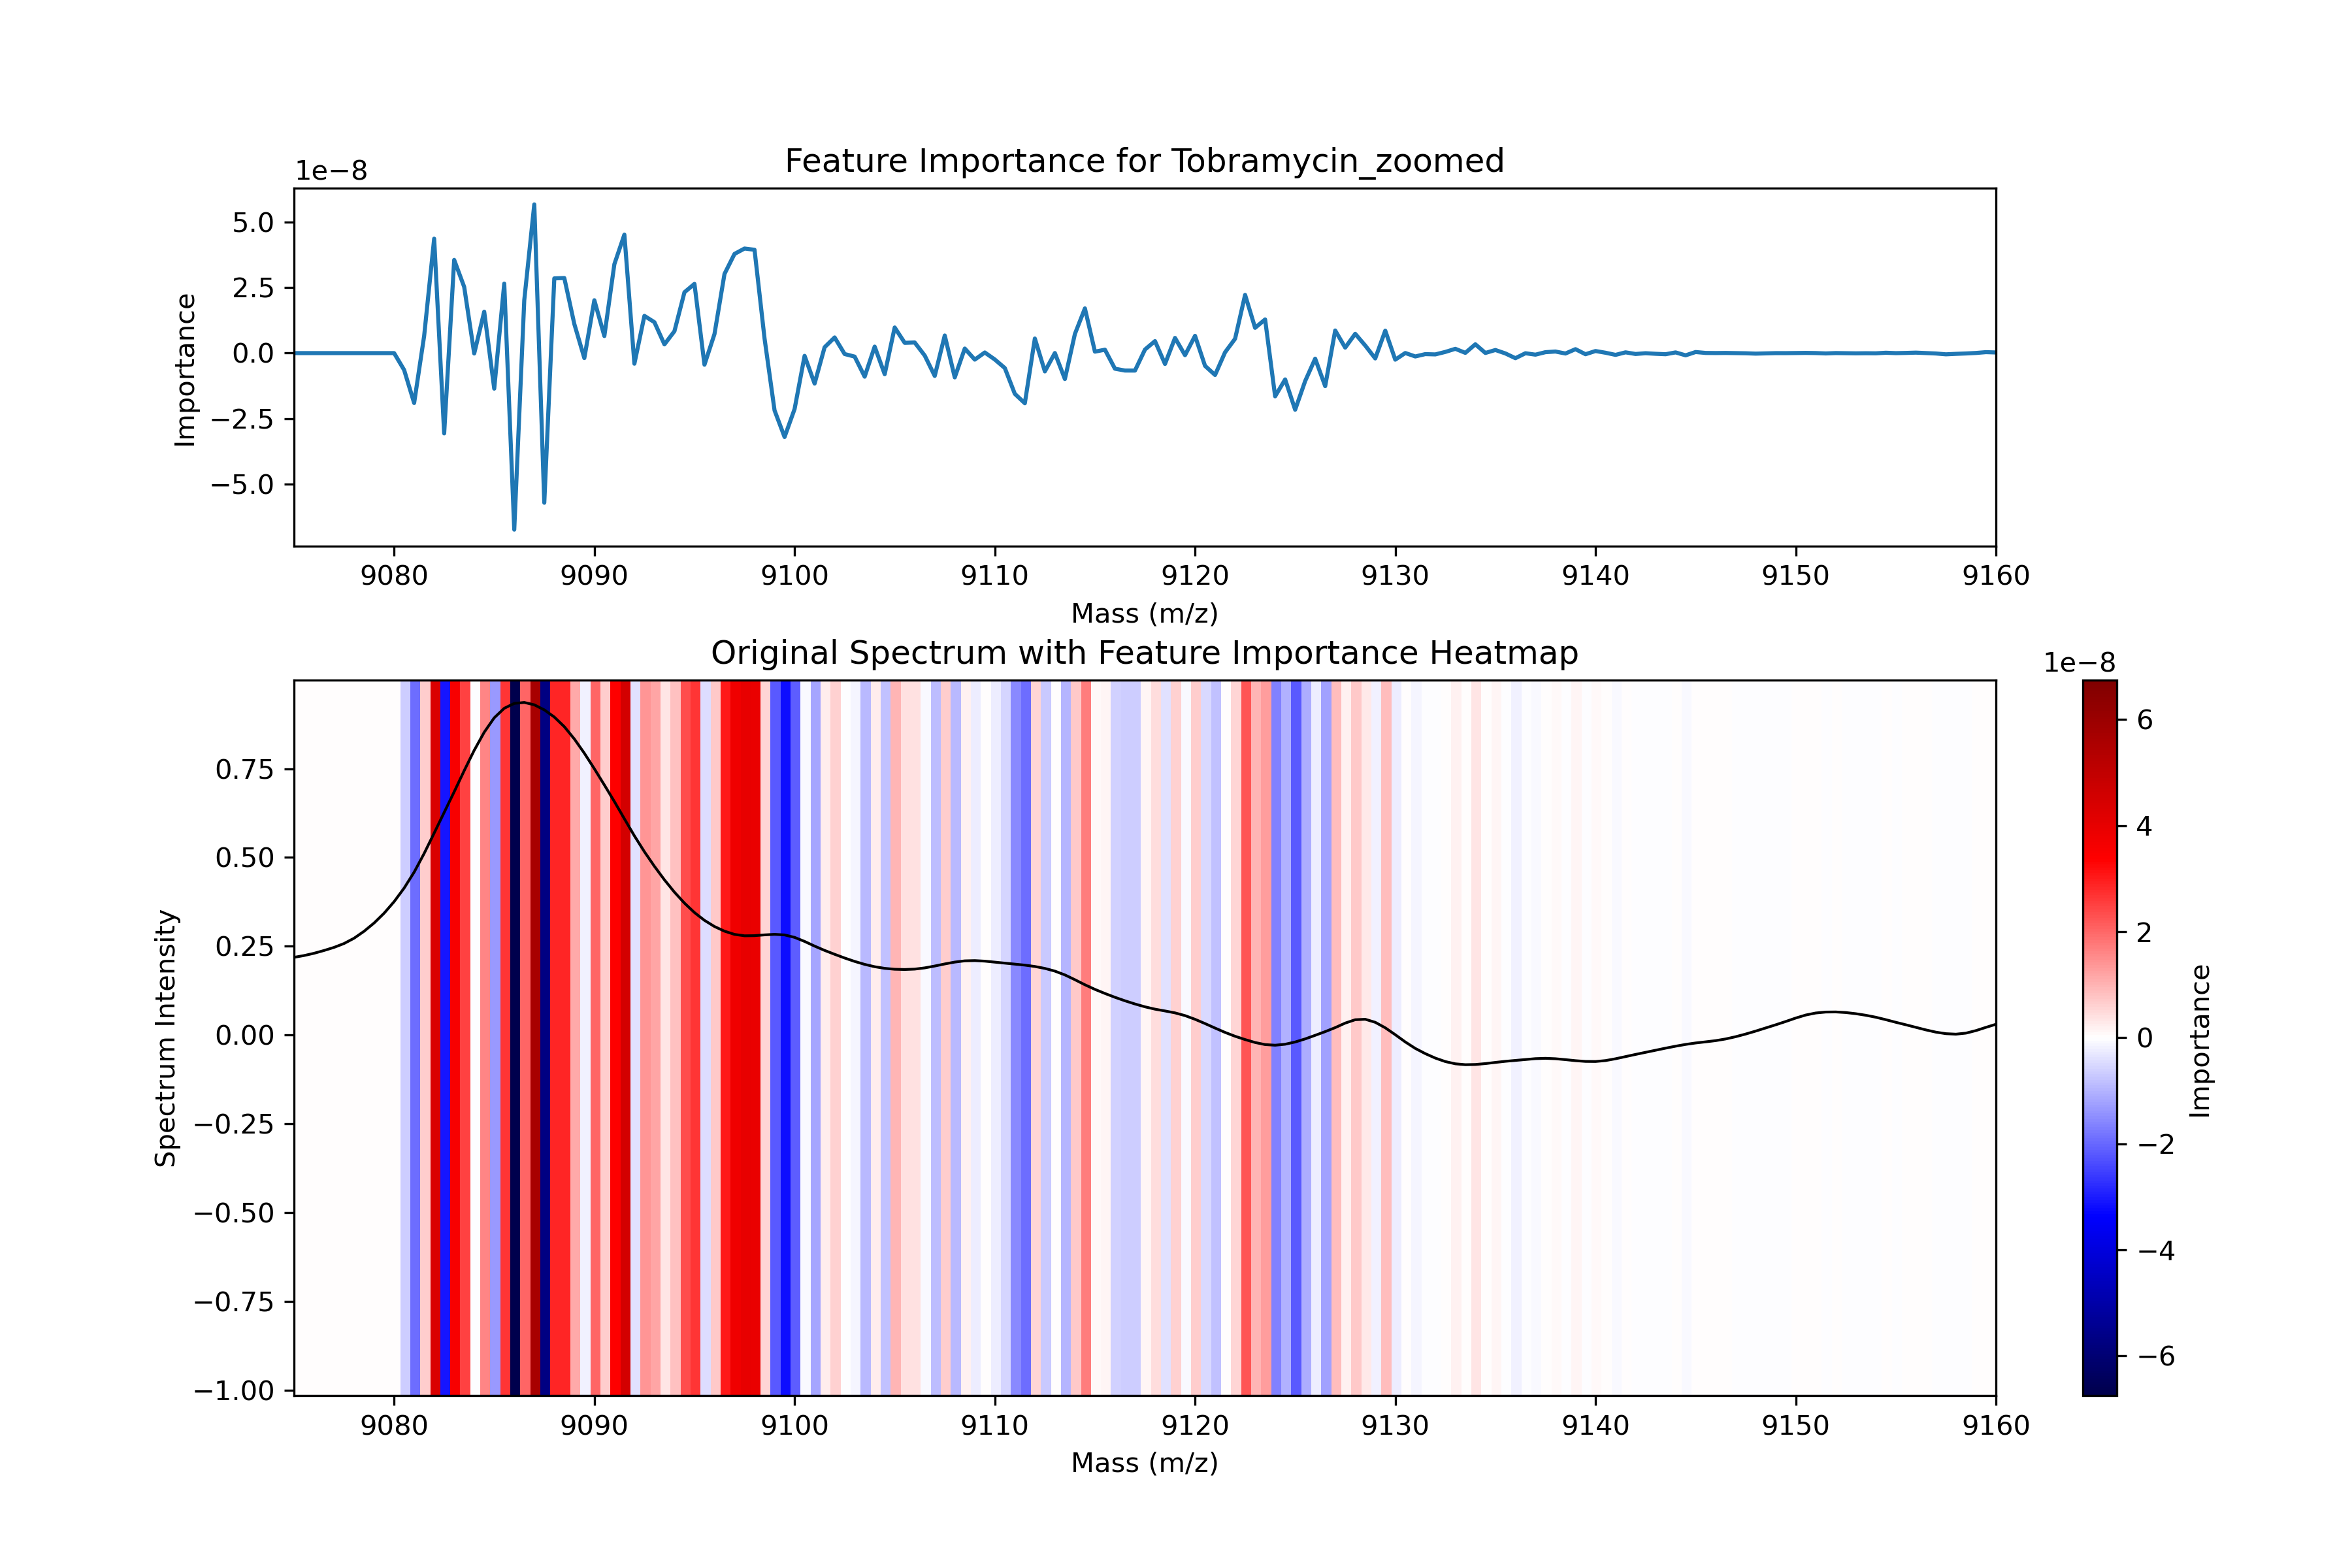
\includegraphics[width=0.9\textwidth]{img/Tobramycin_zoomed.png}
	\caption{Zoomed-in feature importance values derived using GradCAM for Tobramycin resistance around 9085 m/z. The top plot shows the positive and negative feature importances, while the bottom plot overlays these values on the original MALDI-TOF mass spectrum. This detailed view highlights the significant impact of specific spectral features on the model's predictions.}
	\label{fig:tobramycin_zoomed}
\end{figure}

Finally, while other studies have succesfully extracted feature importance maps from various machine learning models \cite{weisDirectAntimicrobialResistance2022,wangRapidDetectionHeterogeneous2018,feucherollesCombinationMALDITOFMass2022}, I have at time of writing not been able to find any studies that have experimentally determined whether or not these feature maps identify relevant proteins that are conducive to resistance. One potential problem with regards to this method is the limitation of MALDI-TOF in terms of its mass detection interval between approximately 2-20 kDa, which mostly includes ribosomal proteins along with certain housekeeping genes (stably expressed genes) \cite{singhalMALDITOFMassSpectrometry2015}. A few  examples of this is, first, the AcrAB-TolC multidrug efflux pump found in \textit{E. coli}  \cite{wangAllostericTransportMechanism2017} which consists of three proteins with masses of 42.2 kDa, 113.6 kDa, and 53.7 kDa, respectively. Similarly there is \( \beta \)-lactamase proteins, that break down Penicillin, with a mass of at least 29 kDa (depending on class) \cite{jelschLactamaseTEM1Coli1992}. However, smaller protein subunits like the AcrZ protein (5.3 kDa) that associates with the aforementioned multidrug efflux pump \cite{hobbsConservedSmallProtein2012} may still be detectable through this method . 

In conclusion, the application of Shapley values and GradCAM in this study not only enhances the interpretability of the CNN model but also provides critical insights into the specific spectral features that drive resistance predictions. These findings underscore the importance of interpretability in machine learning models, particularly in the context of clinical decision-making and antibiotic resistance research.

To illustrate that not all classes are equally easy to determine singular important features for, Clindamycin is shown in Figure \ref{fig:clindamycin_gradcam}. The remaining figures for other antibiotics can be found on the GitHub page linked under the methods section ("Code Availability").

\begin{figure}[h]
	\centering
	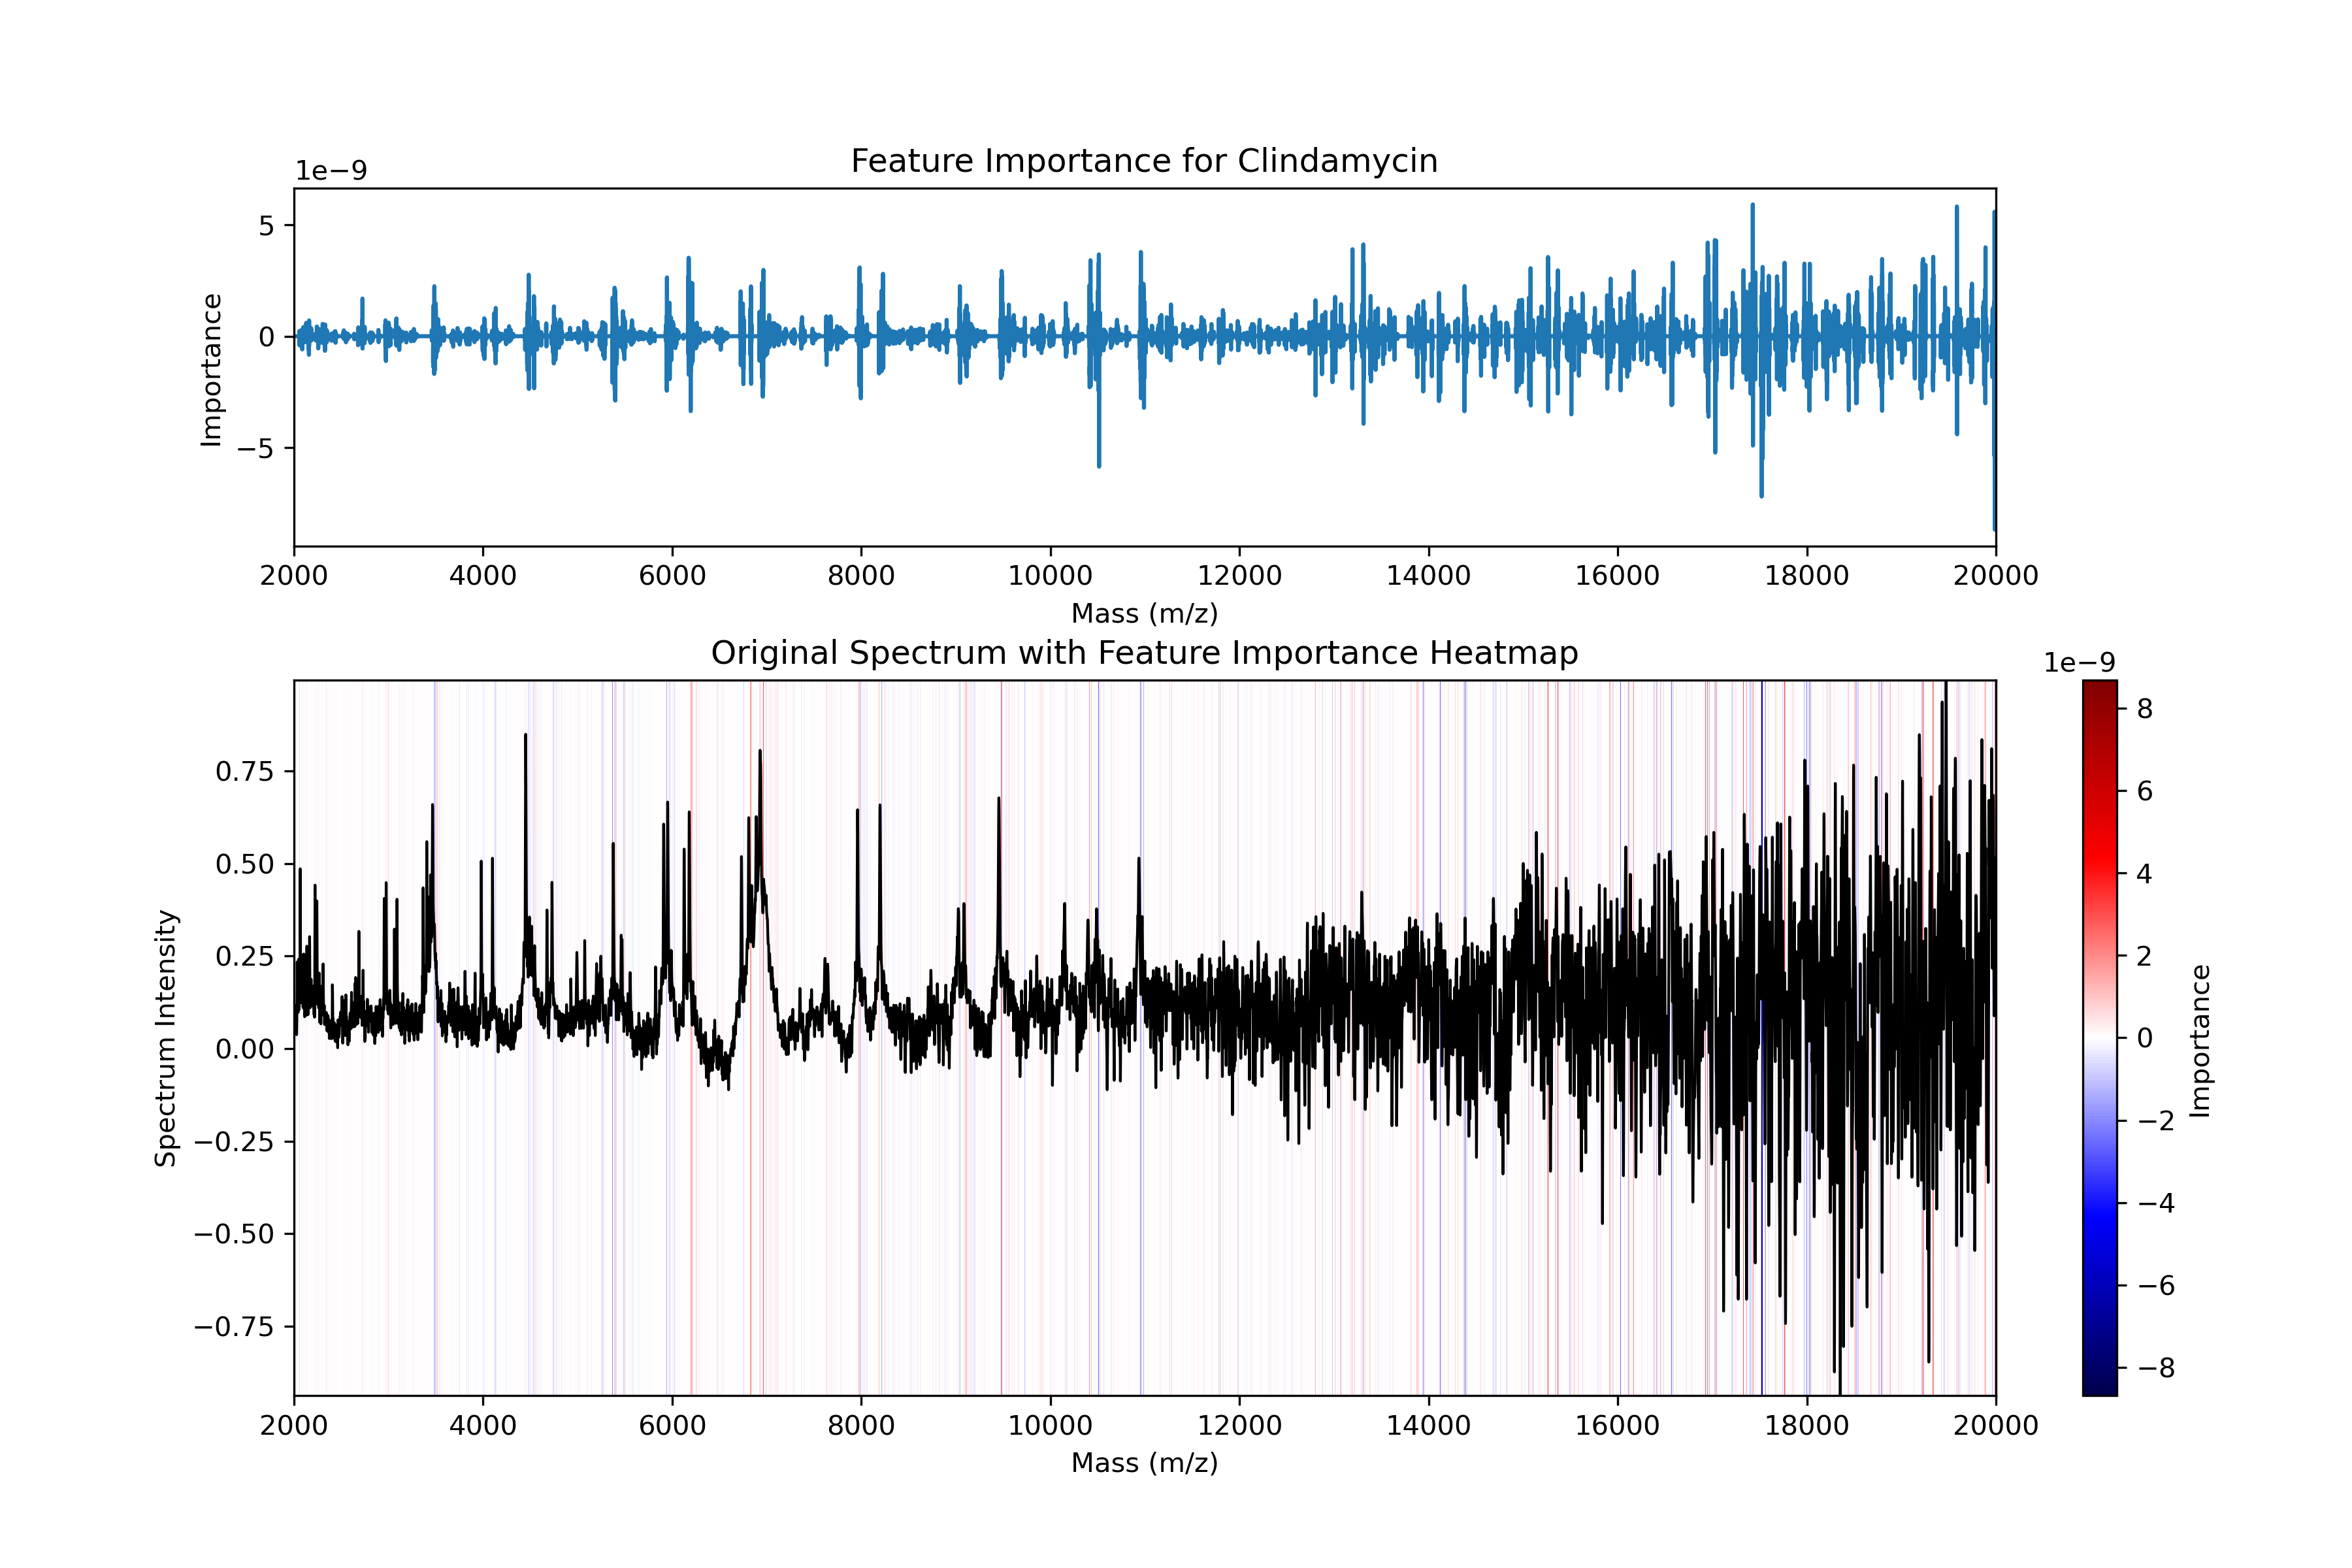
\includegraphics[width=0.9\textwidth]{img/Clindamycin_gradcam.png}
	\caption{Feature importance values derived using GradCAM for a CNN model predicting Clindamycin resistance. The top plot shows Shapley values across the mass spectrum, while the bottom plot overlays these values on the original MALDI-TOF mass spectrum.}
	\label{fig:clindamycin_gradcam}
\end{figure}

\subsubsection*{Future Prospects and Further Work}
The results of this study indicate that both random forest and CNN models show promise in predicting antibiotic resistance, with the CNN model performing slightly better overall. However, to achieve further improvements in predictive performance, it would be beneficial to explore more advanced techniques and methodologies.

One promising direction is the enhancement of existing models. For instance, the Random Forest model could be refined by tuning hyperparameters more rigorously or by employing additional feature engineering. Similarly, the CNN model can be optimized by experimenting with different architectures, to better capture the complex patterns in the mass spectra.

Moreover, alternative machine learning approaches like Transformers and Kolmogorov-Arnold networks (KANs) offer significant potential. The transformer architecture, particularly the Maldi Transformer proposed by De Waele et al. (2024) \cite{dewaelePretrainedMaldiTransformers2024}, is specifically designed for MALDI-TOF MS data and leverages self-supervised pre-training to improve performance on downstream tasks such as antimicrobial resistance prediction. This model addresses some of the limitations of traditional machine learning approaches by directly operating on sets of peaks using permutation-invariant self-attention mechanisms. The pre-training strategy of peak discrimination in Maldi Transformer shows promising results in enhancing predictive performance and robustness against spectra with high levels of background interference.

Similarly, KANs have shown potential in handling high-dimensional data by decomposing complex functions into simpler components \cite{liuKANKolmogorovArnoldNetworks2024}. This approach can be particularly useful in the context of MALDI-TOF data, where the relationship between spectral features and resistance phenotypes can be highly non-linear. By leveraging the expressive power of KANs, it might be possible to capture intricate patterns in the data that are not easily discernible by other models.

Another interesting type of network is the Capsule Network (CapsNet) which is designed to better capture spatial hierarchies in data compared to traditional CNNs \cite{sabourDynamicRoutingCapsules2017}. Where CNNs lose information through pooling, CapsNets preserve information about how parts relate to the whole.

Ultimately, the end goal would be to develop models that can be integrated into clinical workflows for real-time prediction of antibiotic resistance. This requires not only robust model performance, but also efficient and interpretable implementations that clinicians can trust and understand.

\subsection*{Conclusion}
In conclusion, this thesis demonstrates the efficacy of advanced machine learning models, particularly random forests and Convolutional Neural Networks (CNNs), in predicting antibiotic resistance using matrix-assisted laser desorption/ionization time-of-flight mass spectrometry (MALDI-TOF MS) data. Through rigorous preprocessing techniques and the application of Shapley values and GradCAM for feature importance mapping, the models achieved high accuracy and interpretability, crucial for clinical decision-making. While the random forest model exhibited strong performance, the CNN model's slightly superior results and its ability to provide detailed feature mappings underscore its potential. However, the study also highlights the importance of continuing to refine these models and exploring alternative approaches to further enhance predictive capabilities. Future work should also focus on experimental validation of identified spectral features and expanding datasets to improve generalizability. Overall, the findings emphasize the significant potential of machine learning in combating antimicrobial resistance, paving the way for more accurate and reliable diagnostic tools.

\newpage
\printbibliography

\clearpage
\renewcommand{\thefigure}{S\arabic{figure}}
\renewcommand{\figurename}{}
\setcounter{figure}{0}

\section*{Supplementary Materials}

\begin{sidewaysfigure}
	\centering
	\begin{minipage}[b!]{0.8\textwidth}
		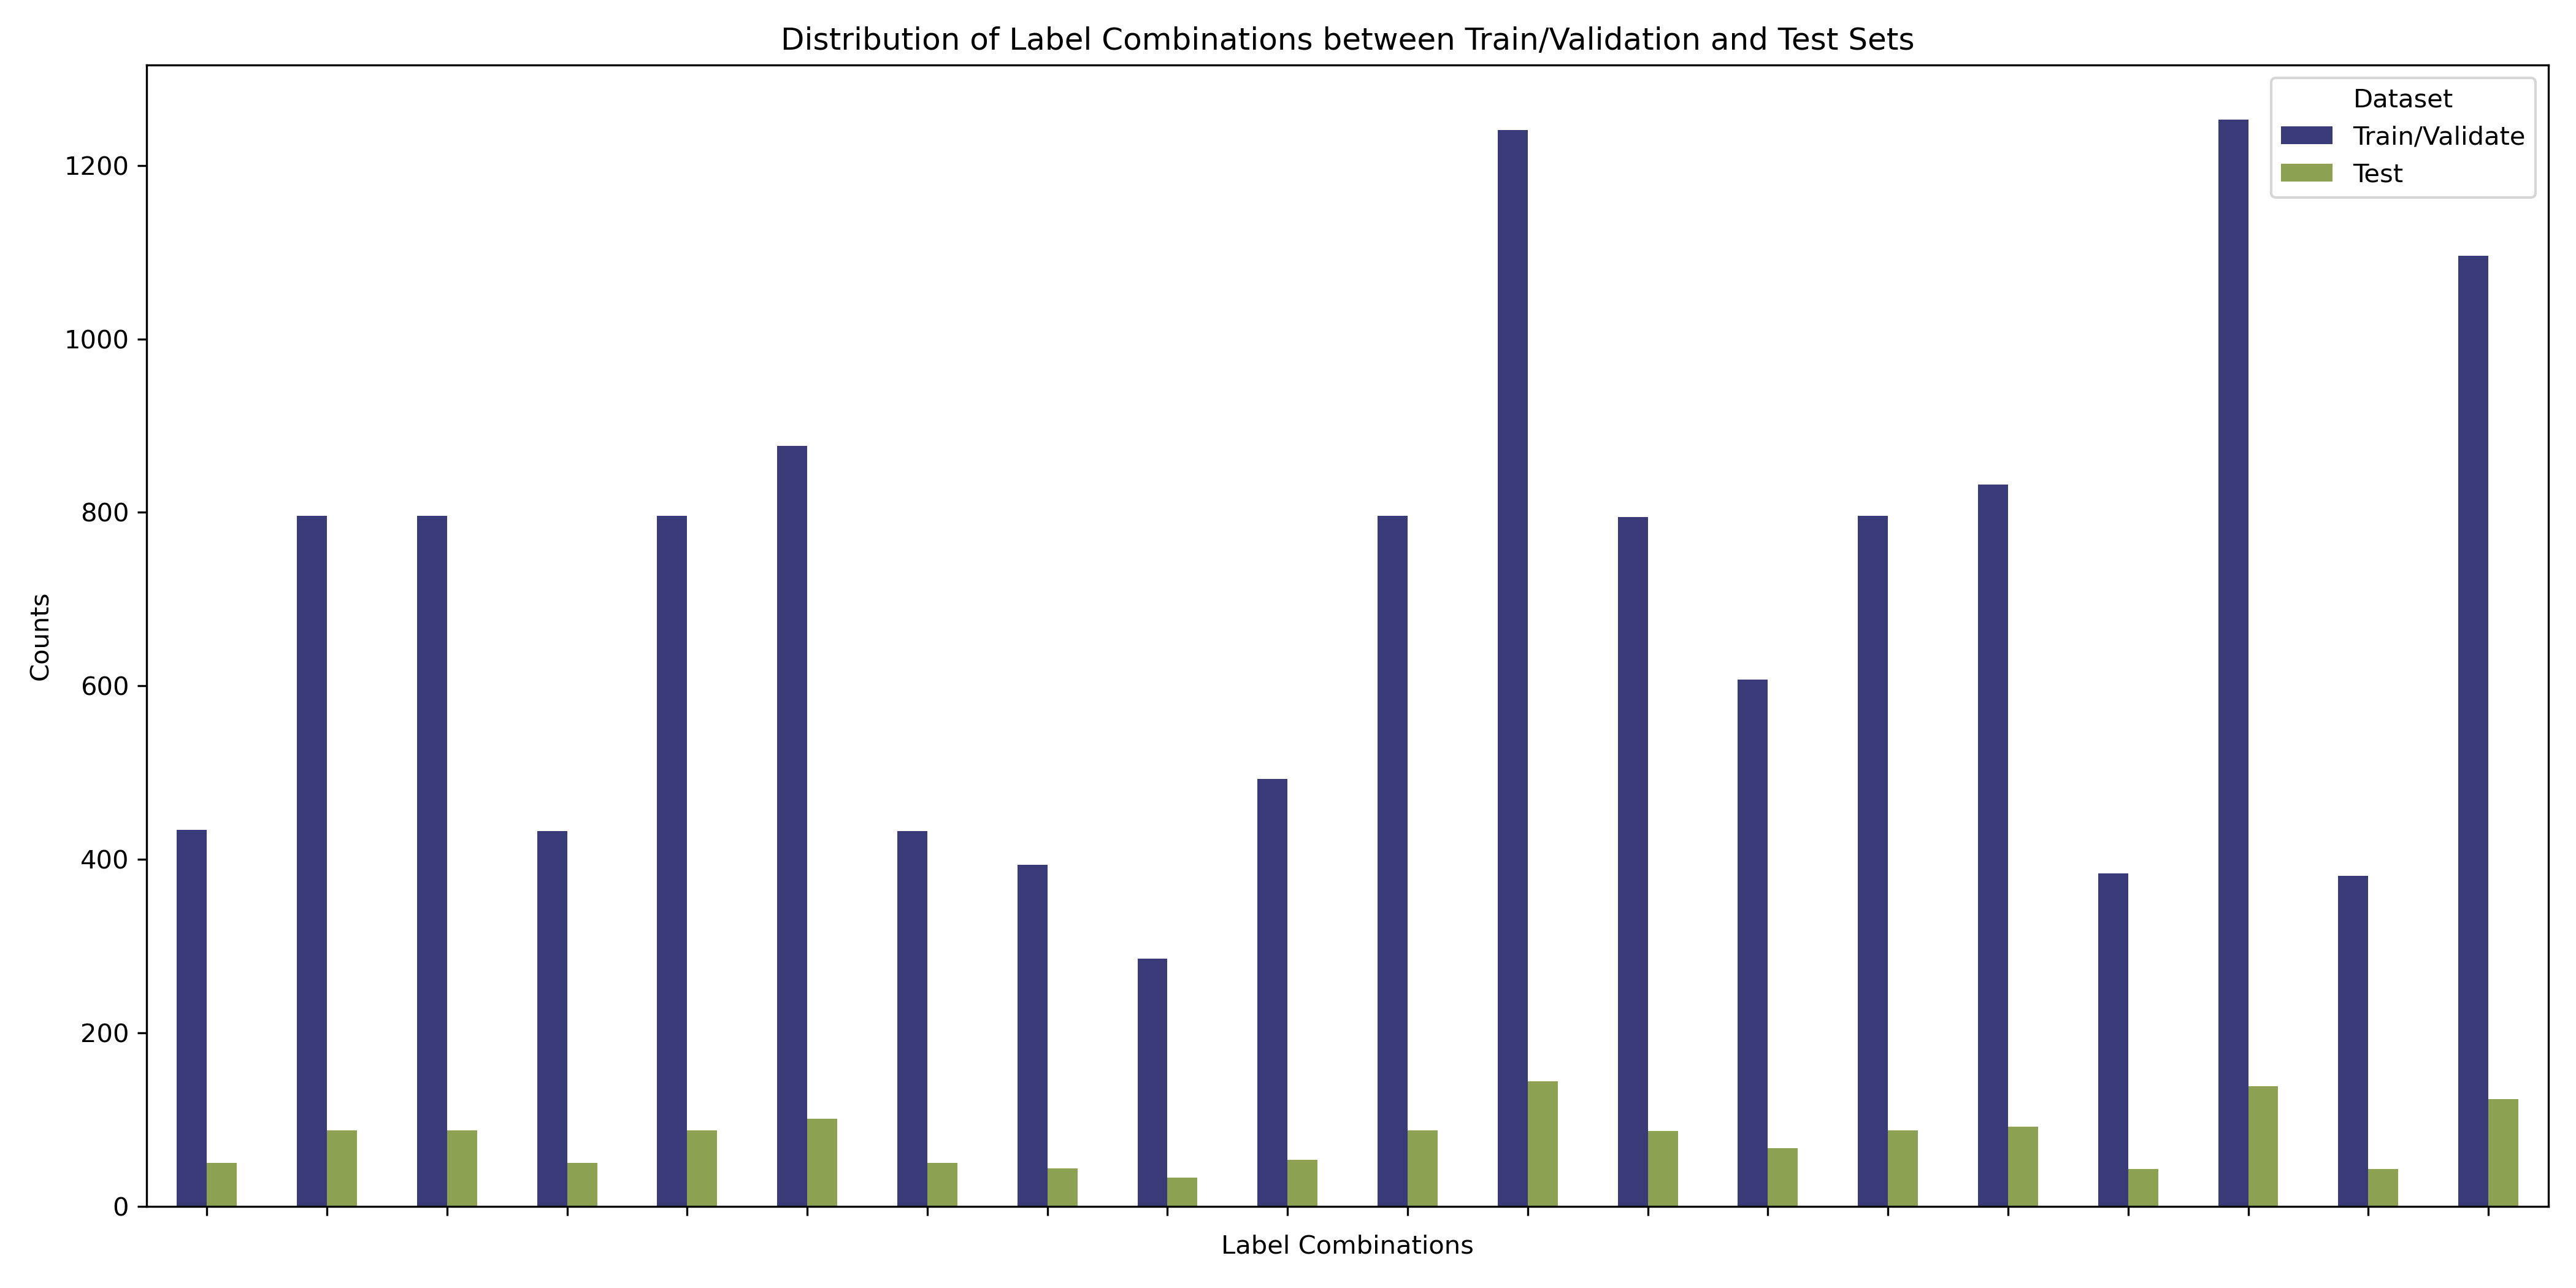
\includegraphics[width=\textwidth]{img/2018_train_val_test_split.png}
		\captionsetup{font=small}
		\caption{Distribution of Label Combinations between Train/Validation and Test Sets. The bar plot shows the frequency of some of the label combinations in the training/validation set (blue) and the test set (green). The x-axis represents the different label combinations, while the y-axis indicates the count of each combination in the respective datasets. This visualization demonstrates that the stratified split maintains the distribution of label combinations across the train/validation and test sets, ensuring that the datasets are representative of each other.}
		\label{fig:multilabel_split}
	\end{minipage}
\end{sidewaysfigure}
\clearpage

\begin{figure}[h]
	\centering
	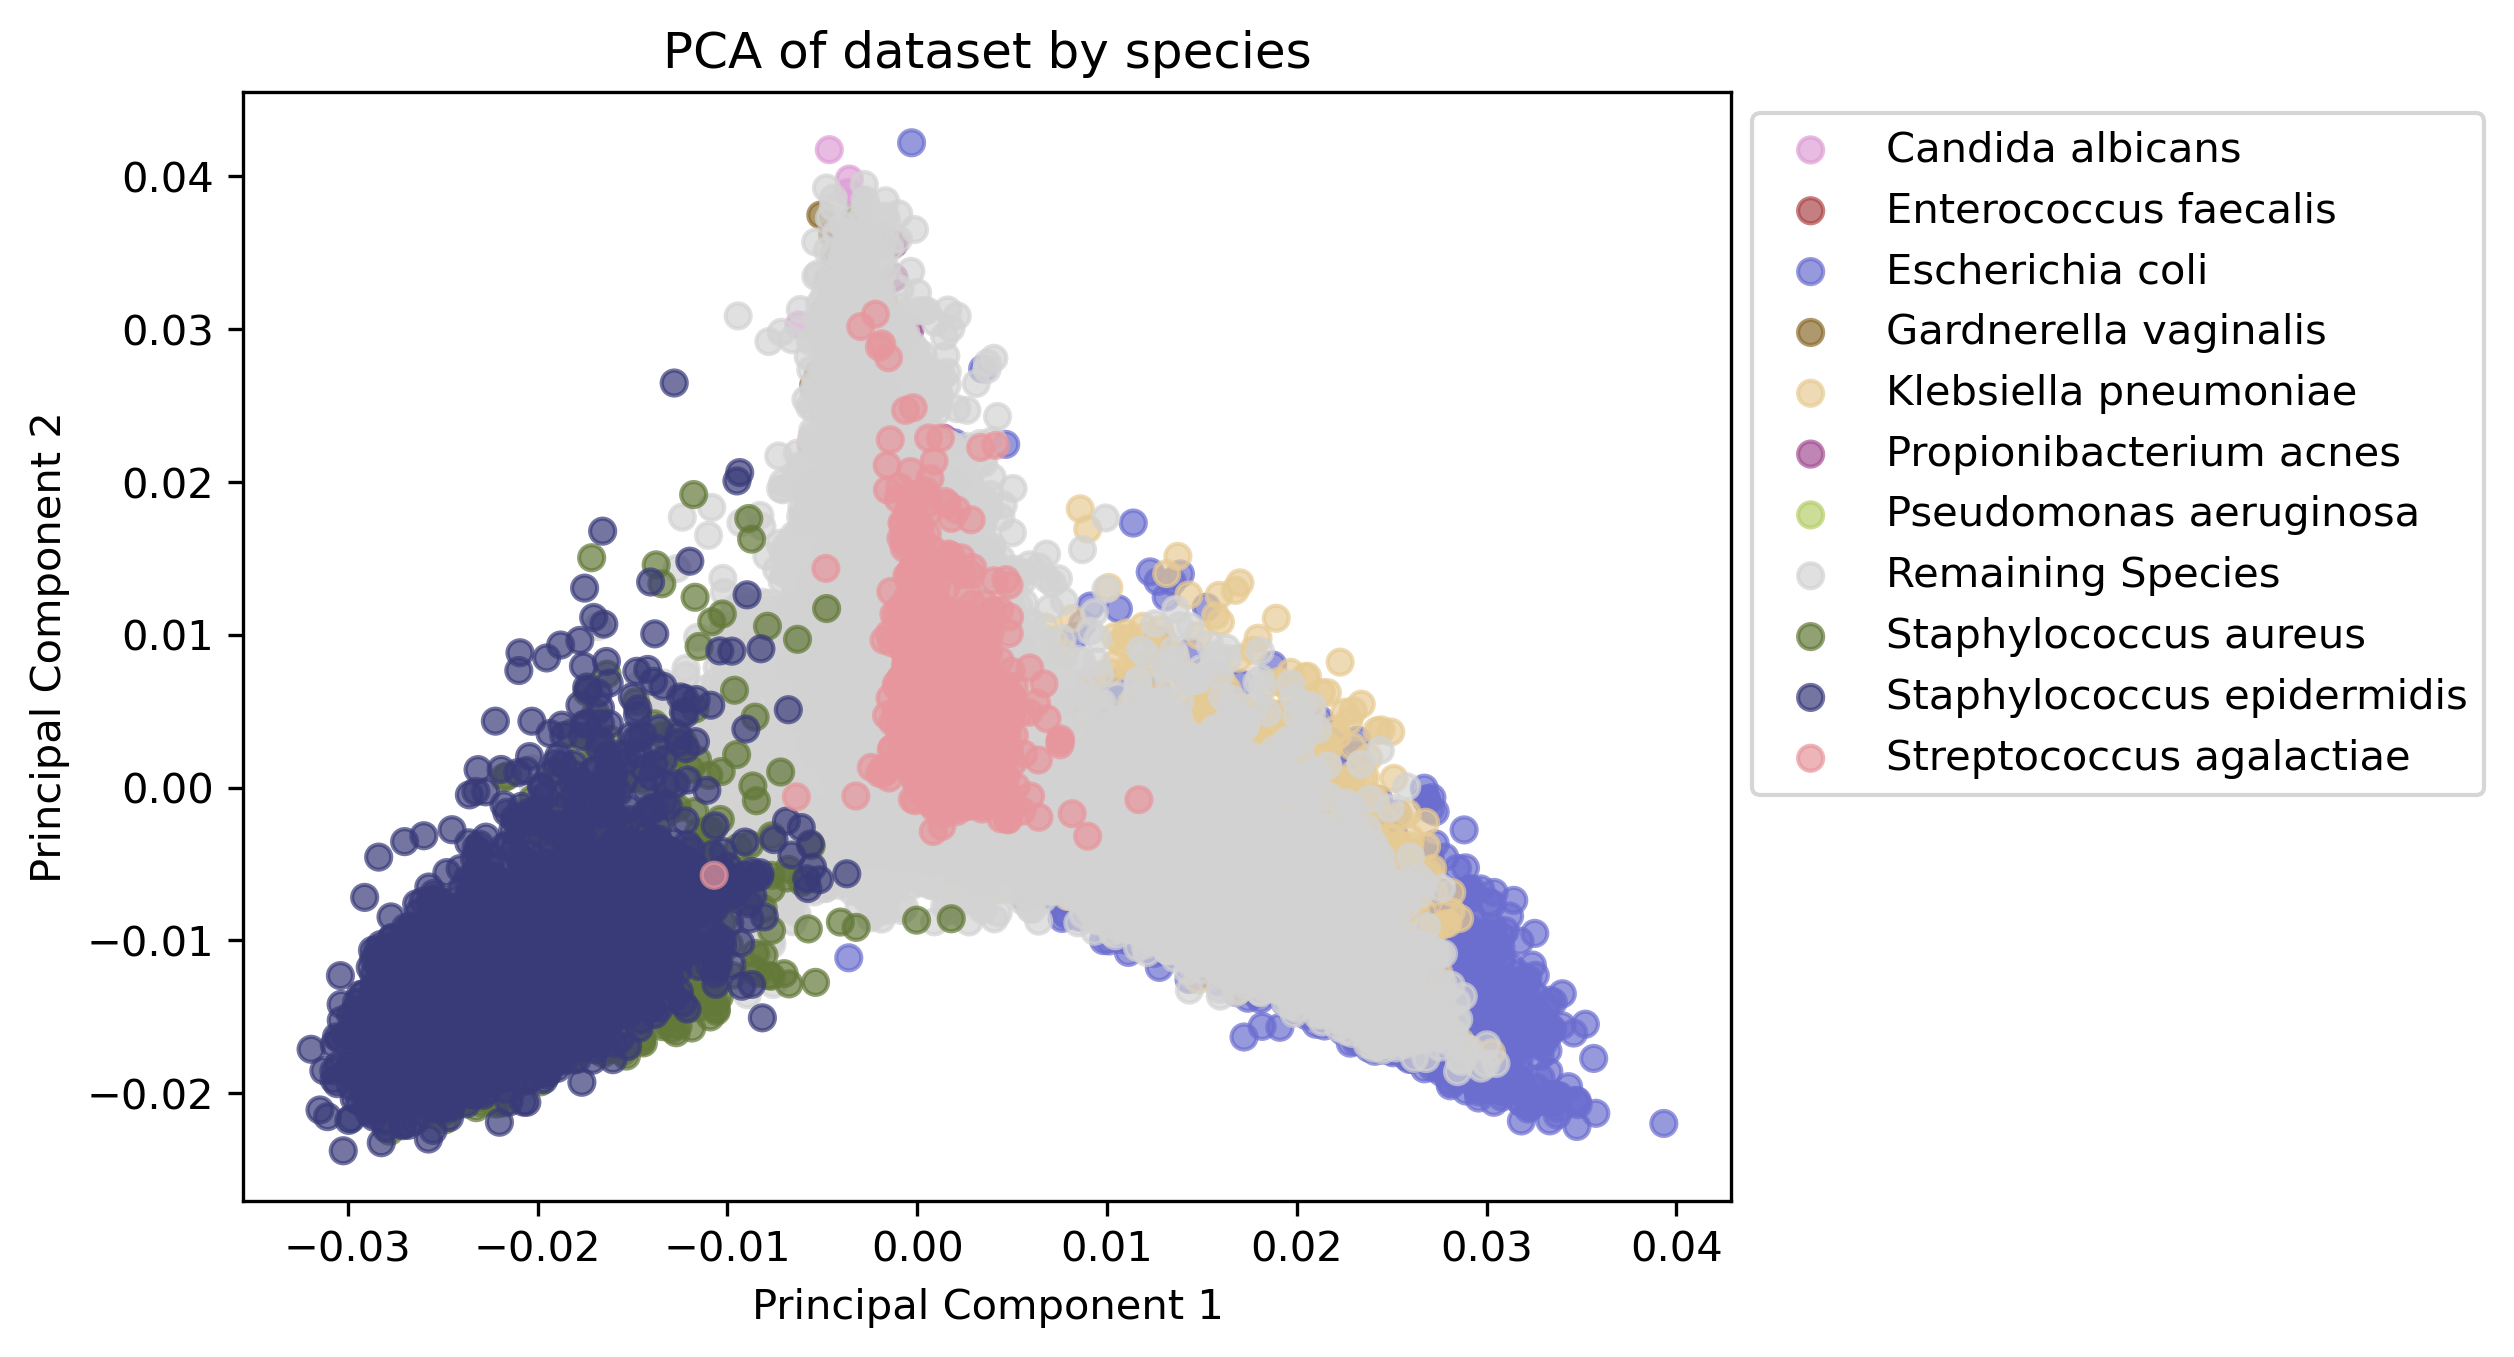
\includegraphics[width=0.9\textwidth]{img/PCA_species.png}
	\caption{Principal Components 1 and 2 from the 2017 dataset by species, including 'Remaining Species' which consists of all species outside the top 10.}
	\label{fig:pca_remaining}
\end{figure}


\begin{figure}[h]
	\centering
	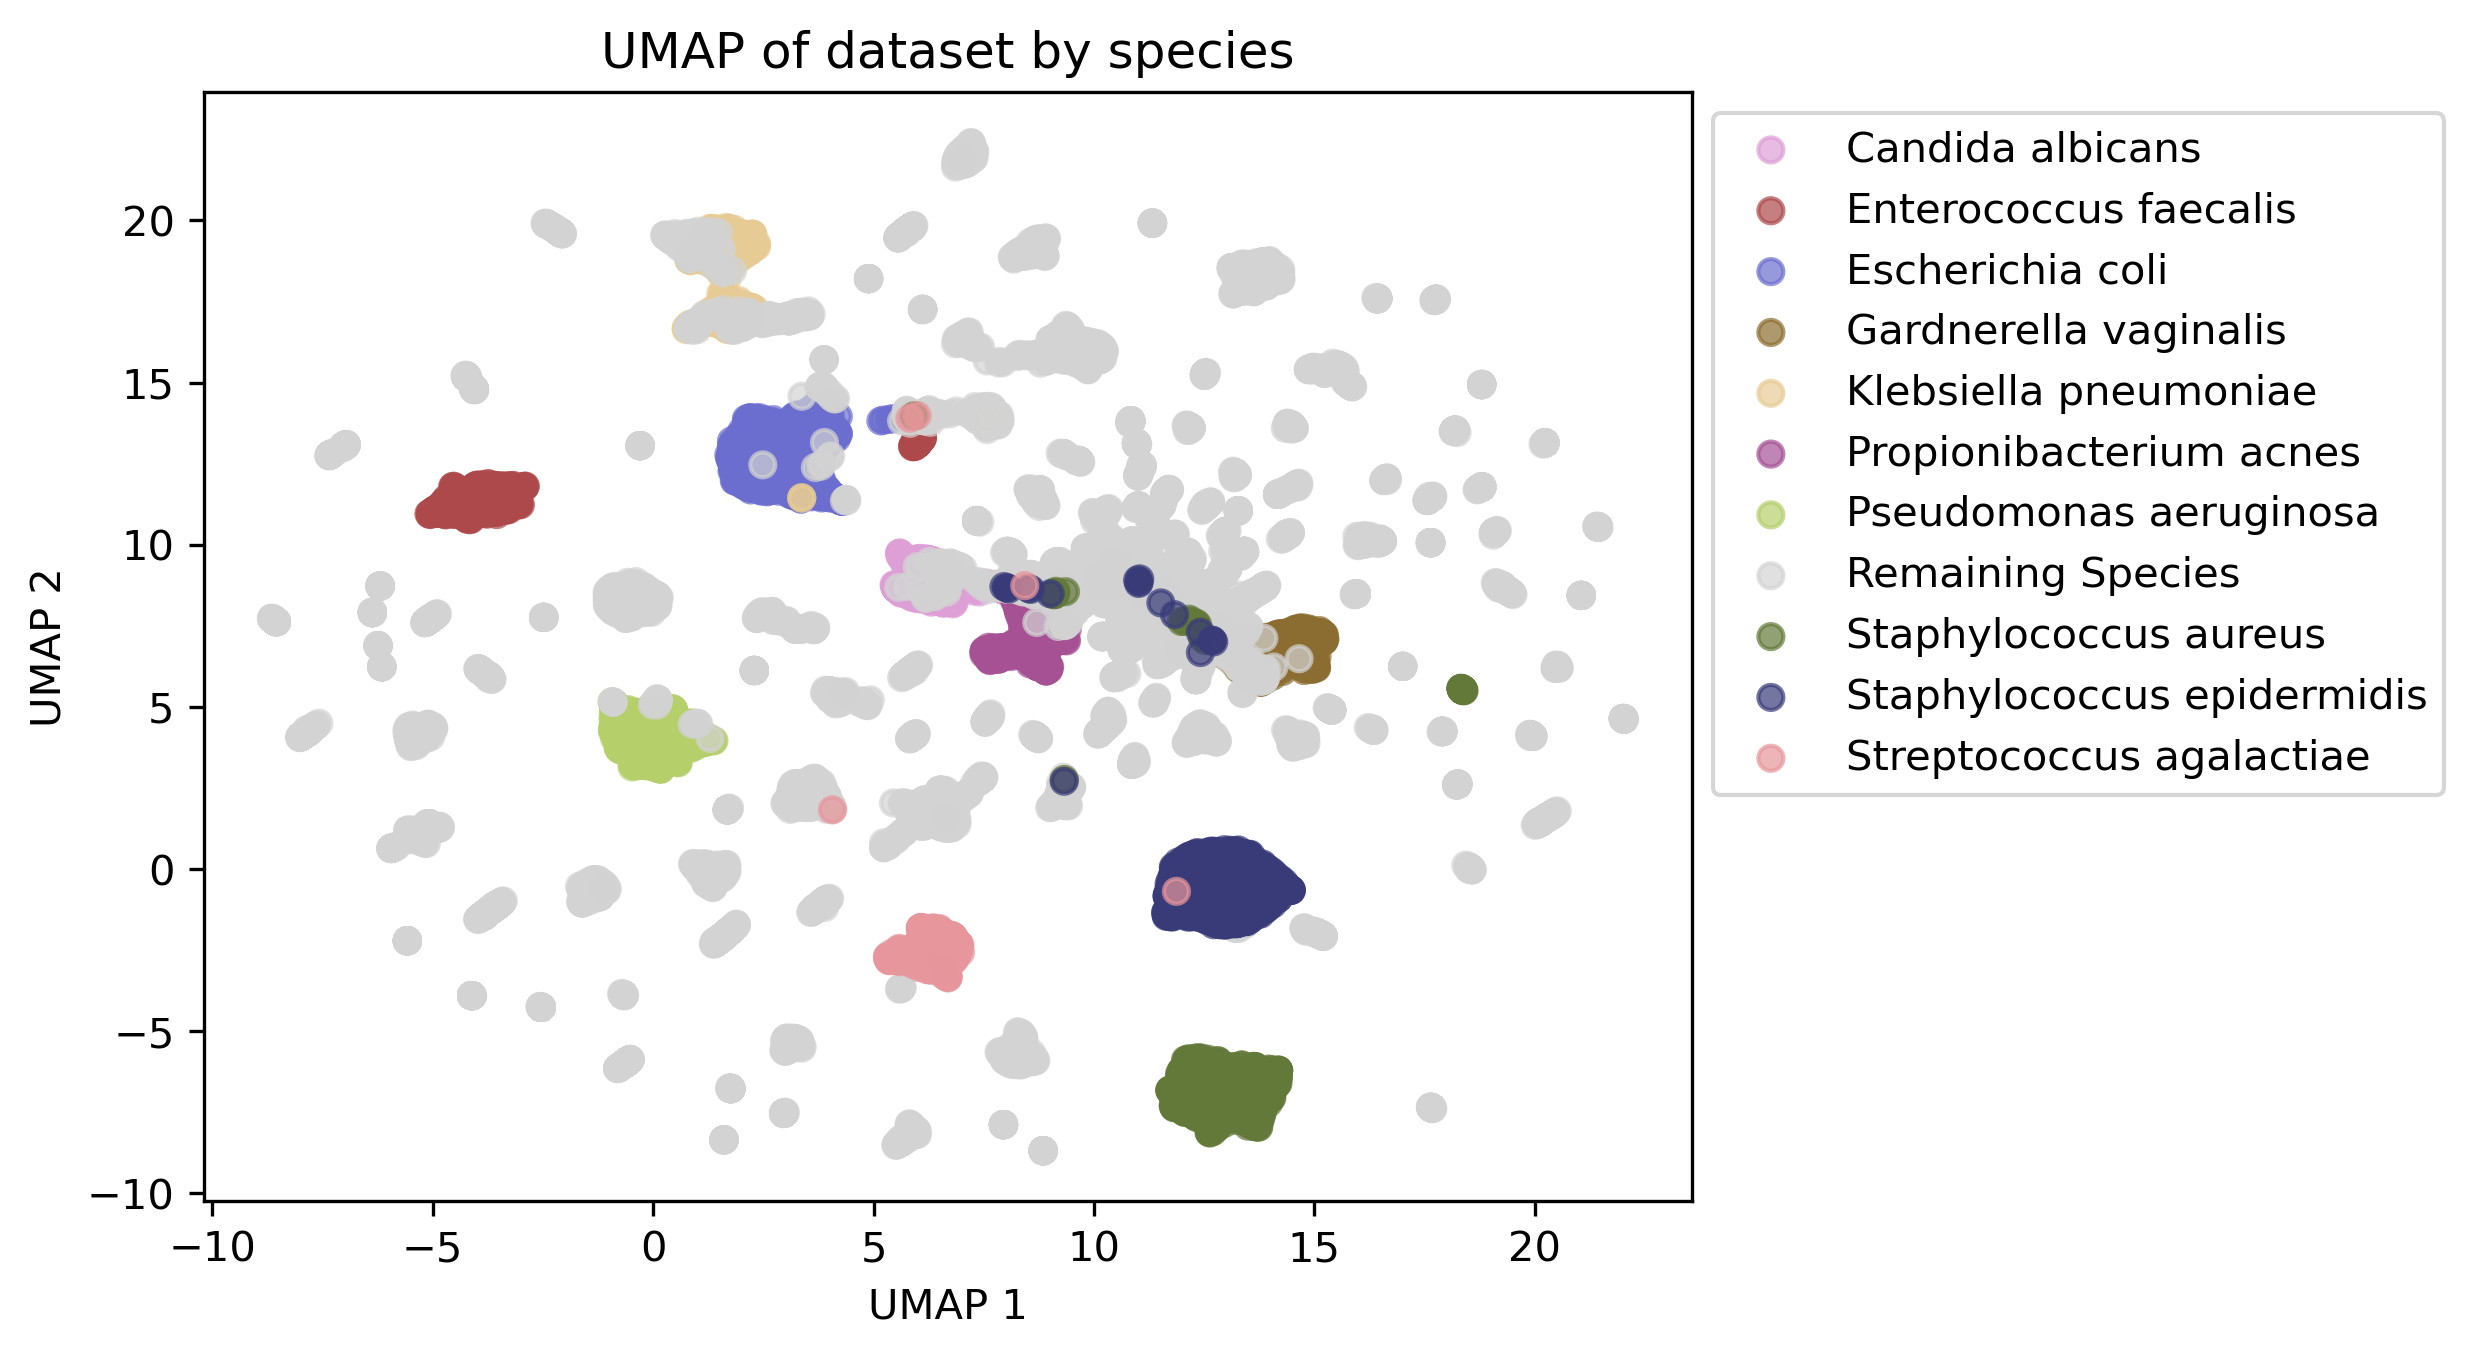
\includegraphics[width=0.9\textwidth]{img/UMAP_species.png}
	\caption{UMAP of the 2017 dataset by species, including 'Remaining Species' which consists of all species outside the top 10.}
	\label{fig:umap_remaining}
\end{figure}

\begin{figure}[h]
	\centering
	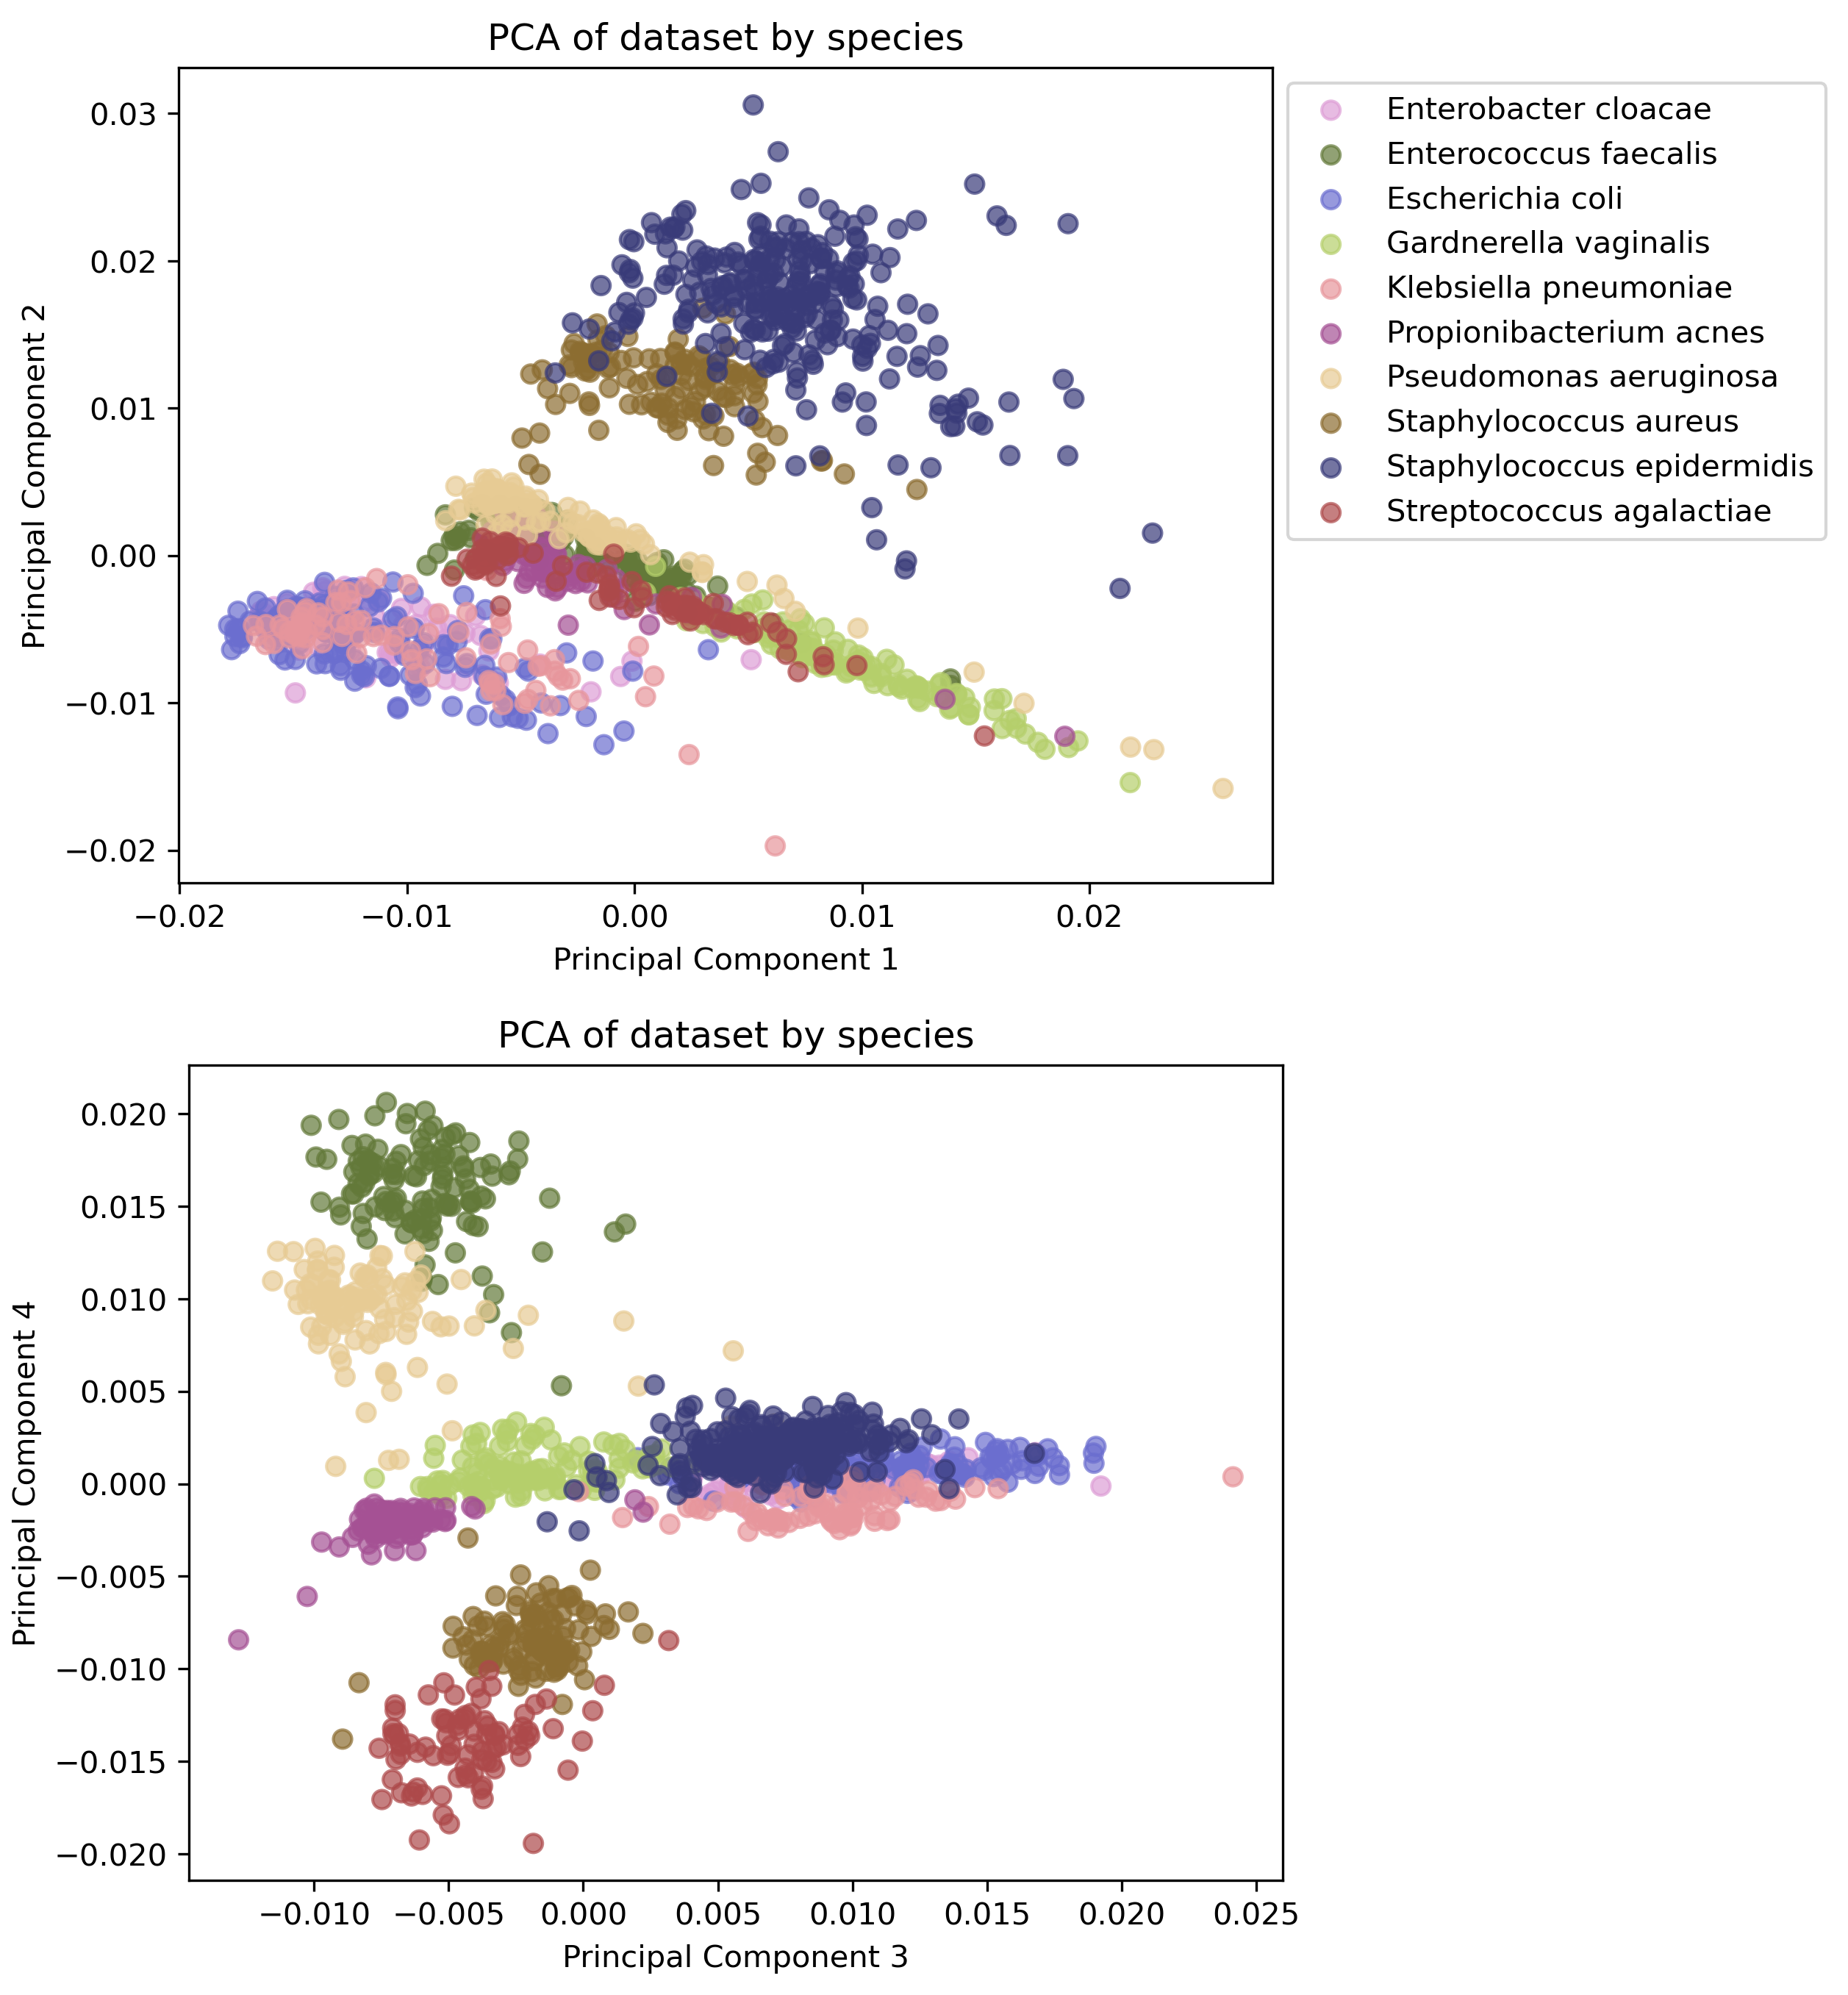
\includegraphics[width=0.9\textwidth]{img/PCA_species_2015.png}
	\caption{Principal Component Analysis (PCA) of the 2015 dataset by species.}
	\label{fig:pca_2015}
\end{figure}

\begin{figure}[h]
	\centering
	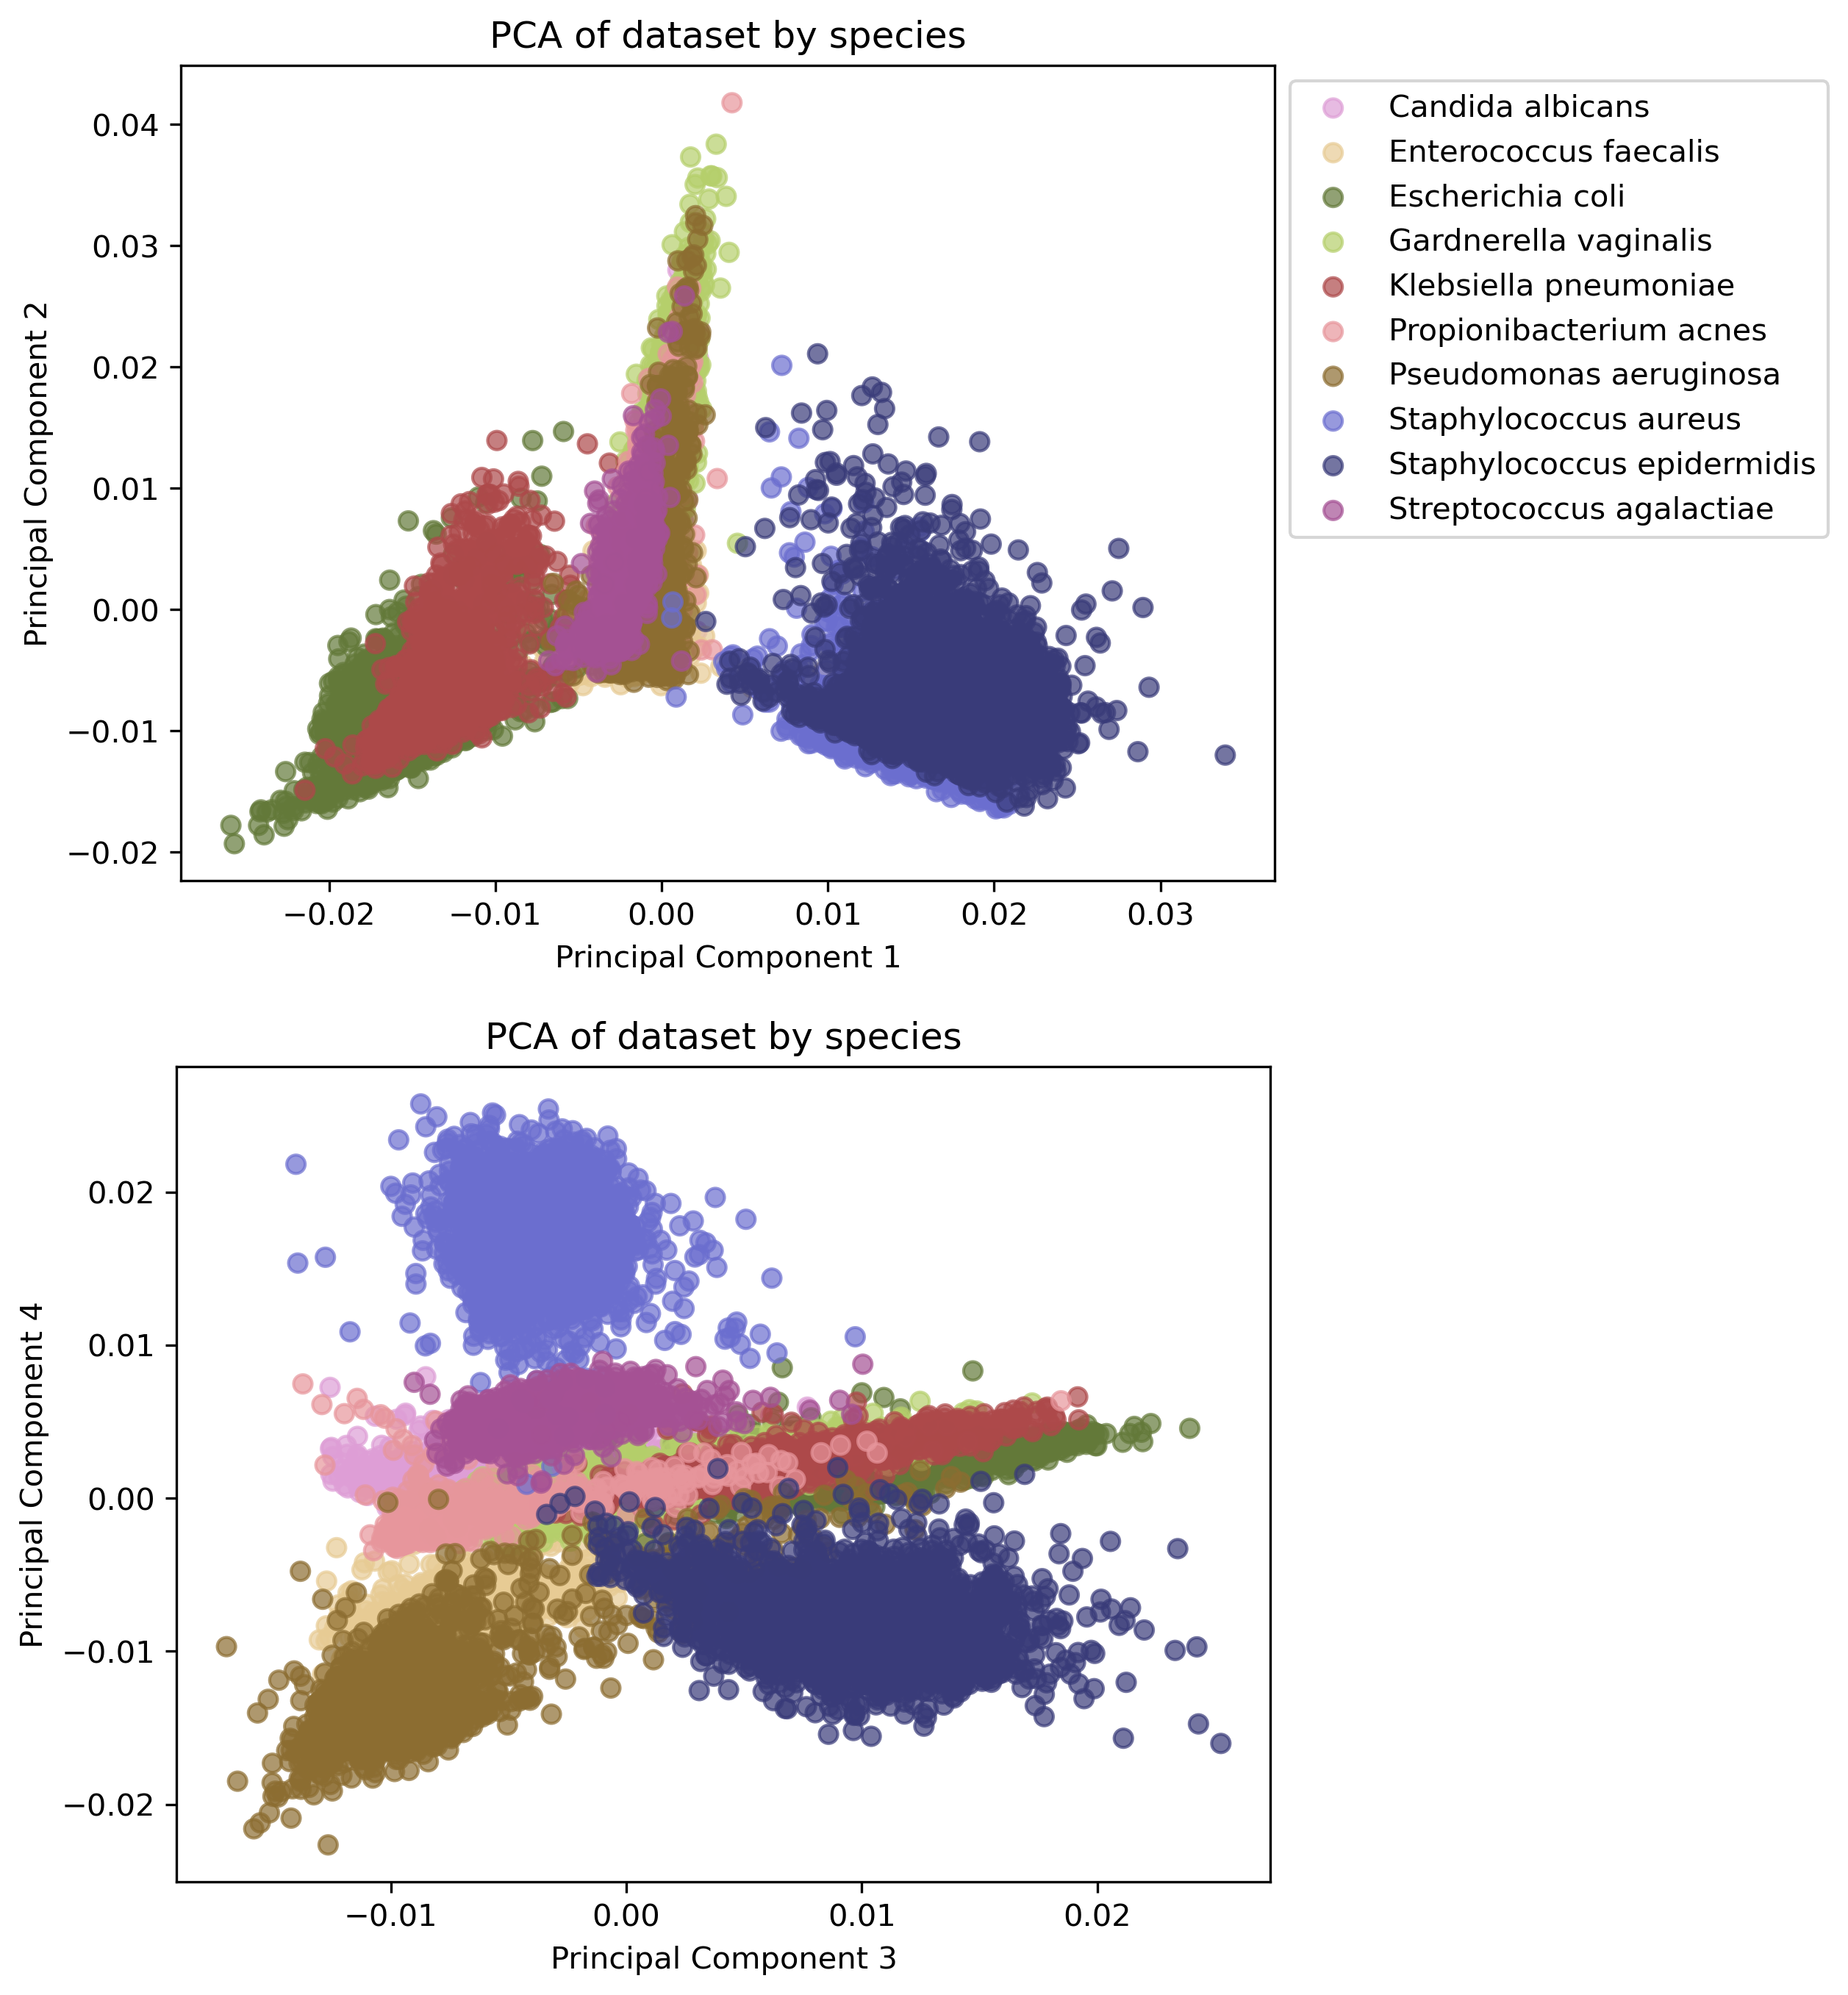
\includegraphics[width=0.9\textwidth]{img/PCA_species_2016.png}
	\caption{Principal Component Analysis (PCA) of the 2016 dataset by species.}
	\label{fig:pca_2016}
\end{figure}

\begin{figure}[h]
	\centering
	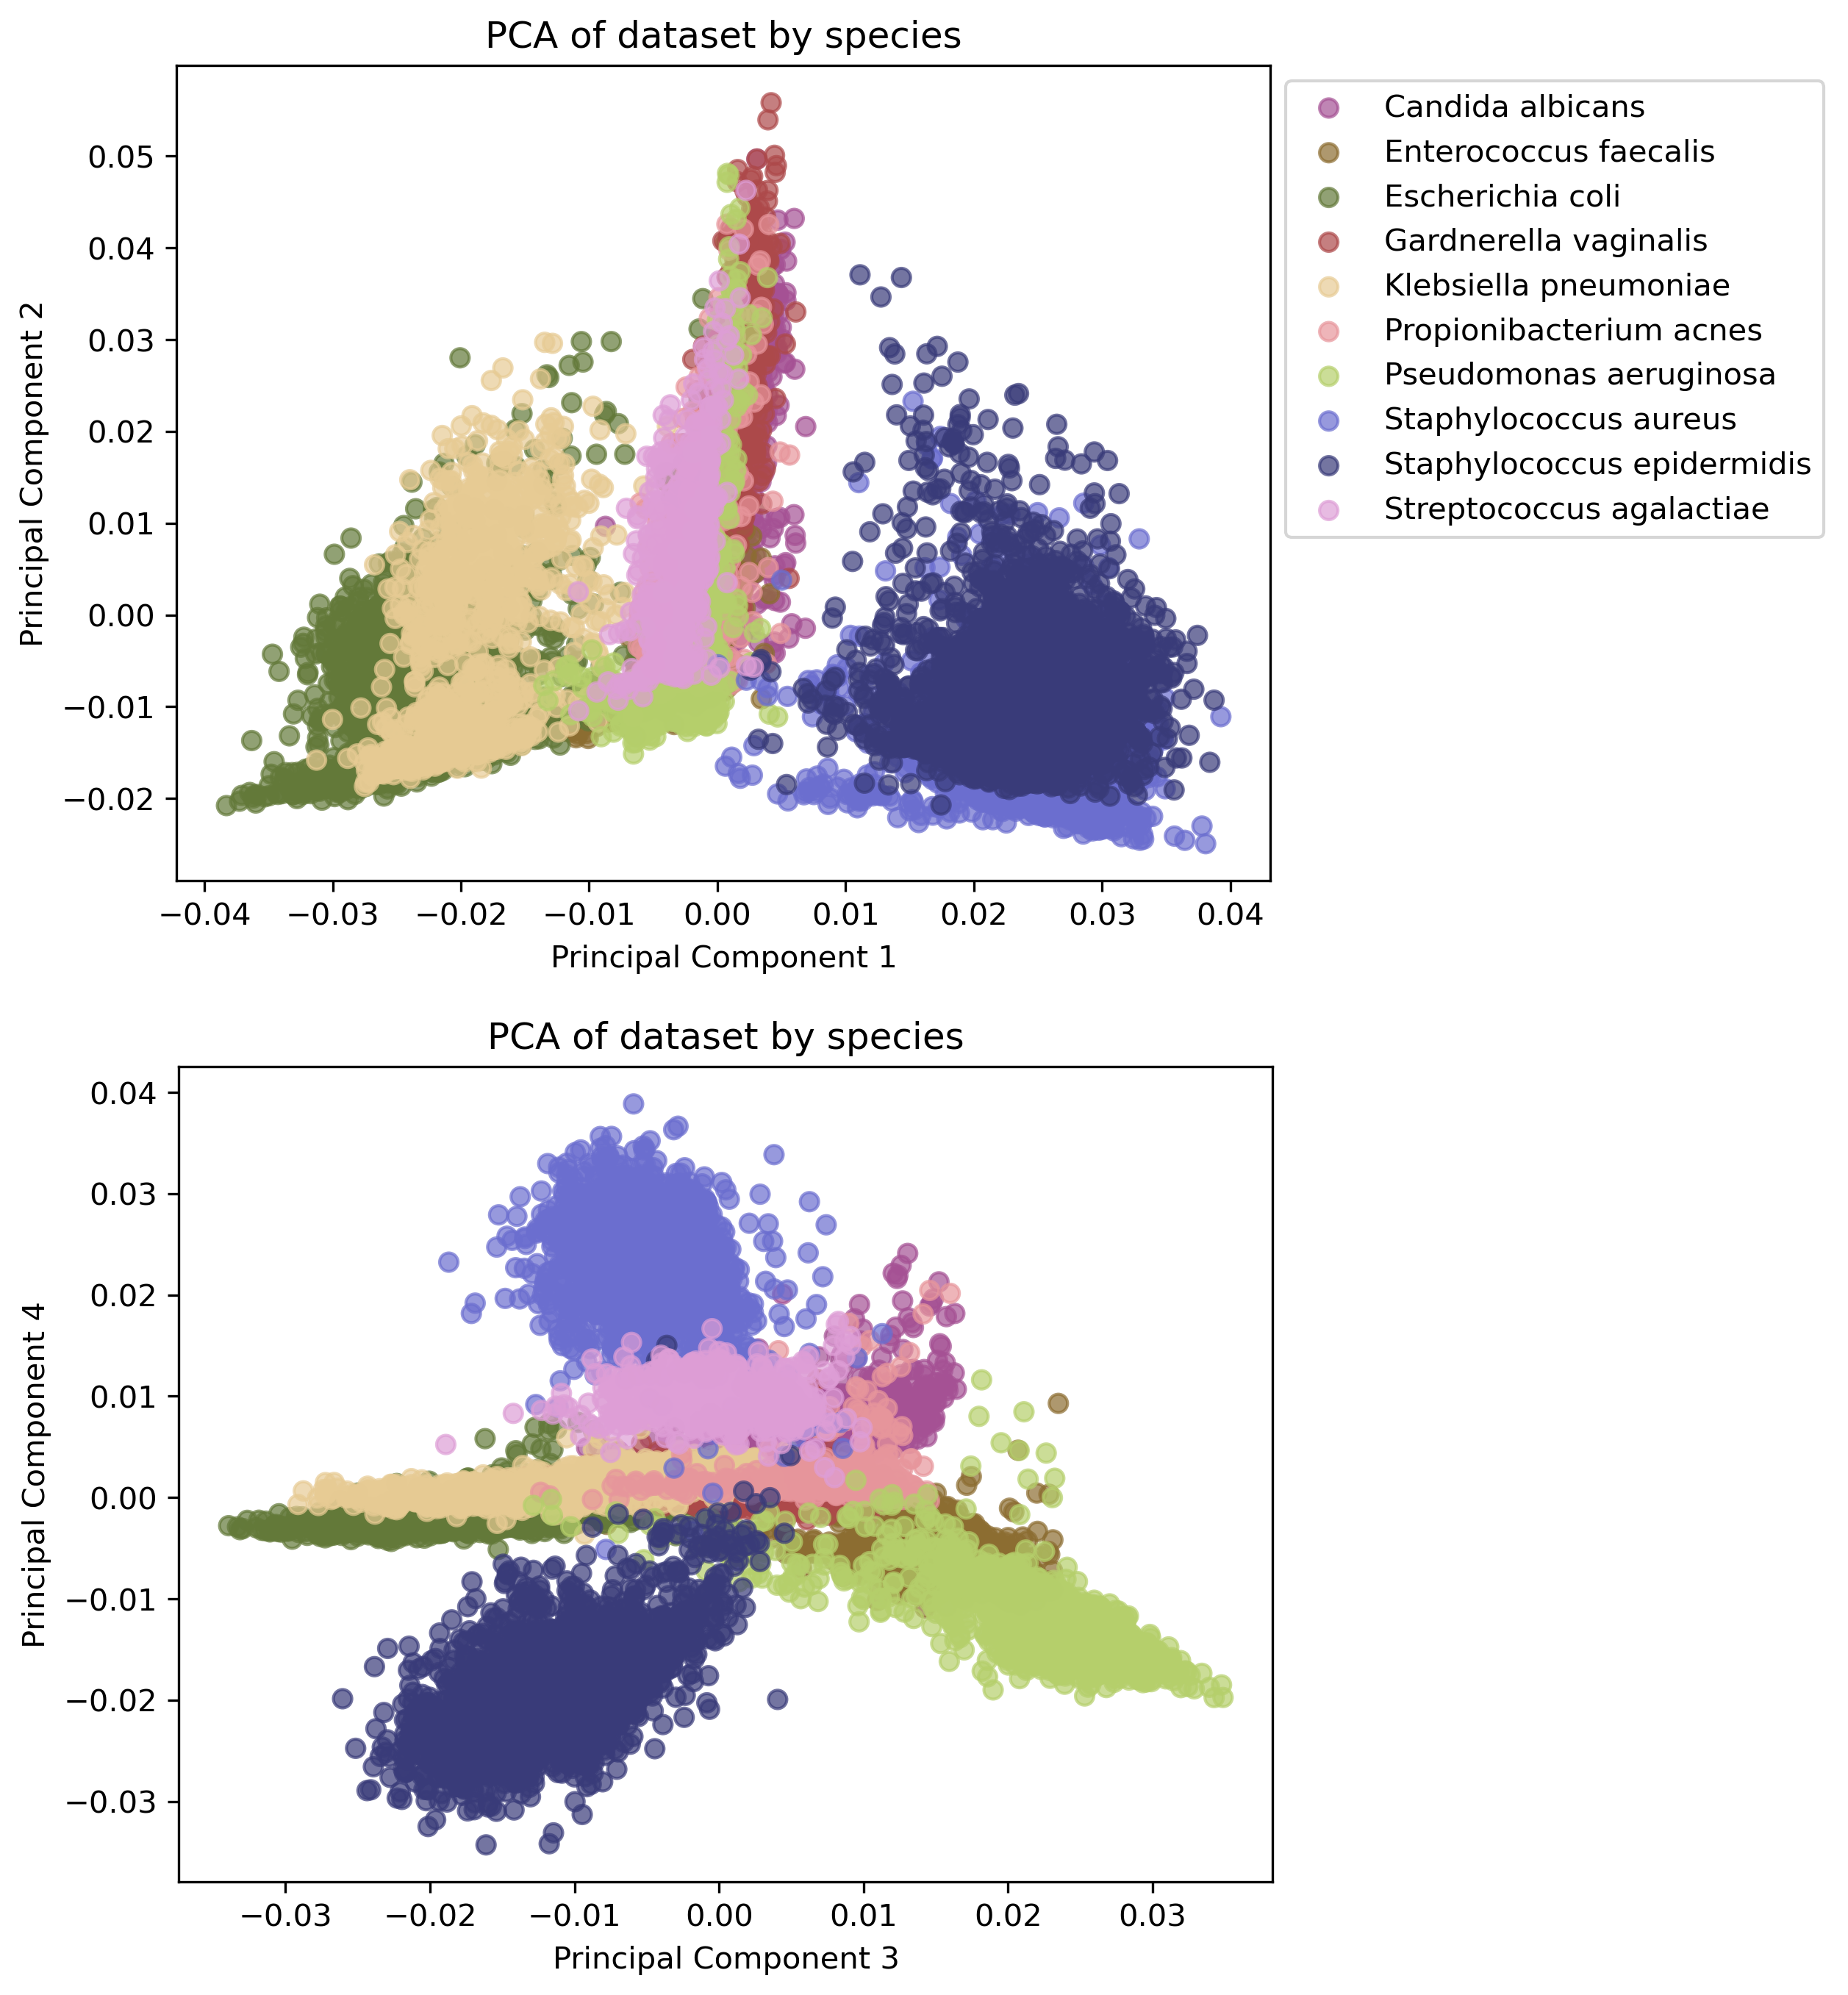
\includegraphics[width=0.9\textwidth]{img/PCA_species_2018.png}
	\caption{Principal Component Analysis (PCA) of the 2018 dataset by species.}
	\label{fig:pca_2018}
\end{figure}

\begin{figure}[h]
	\centering
	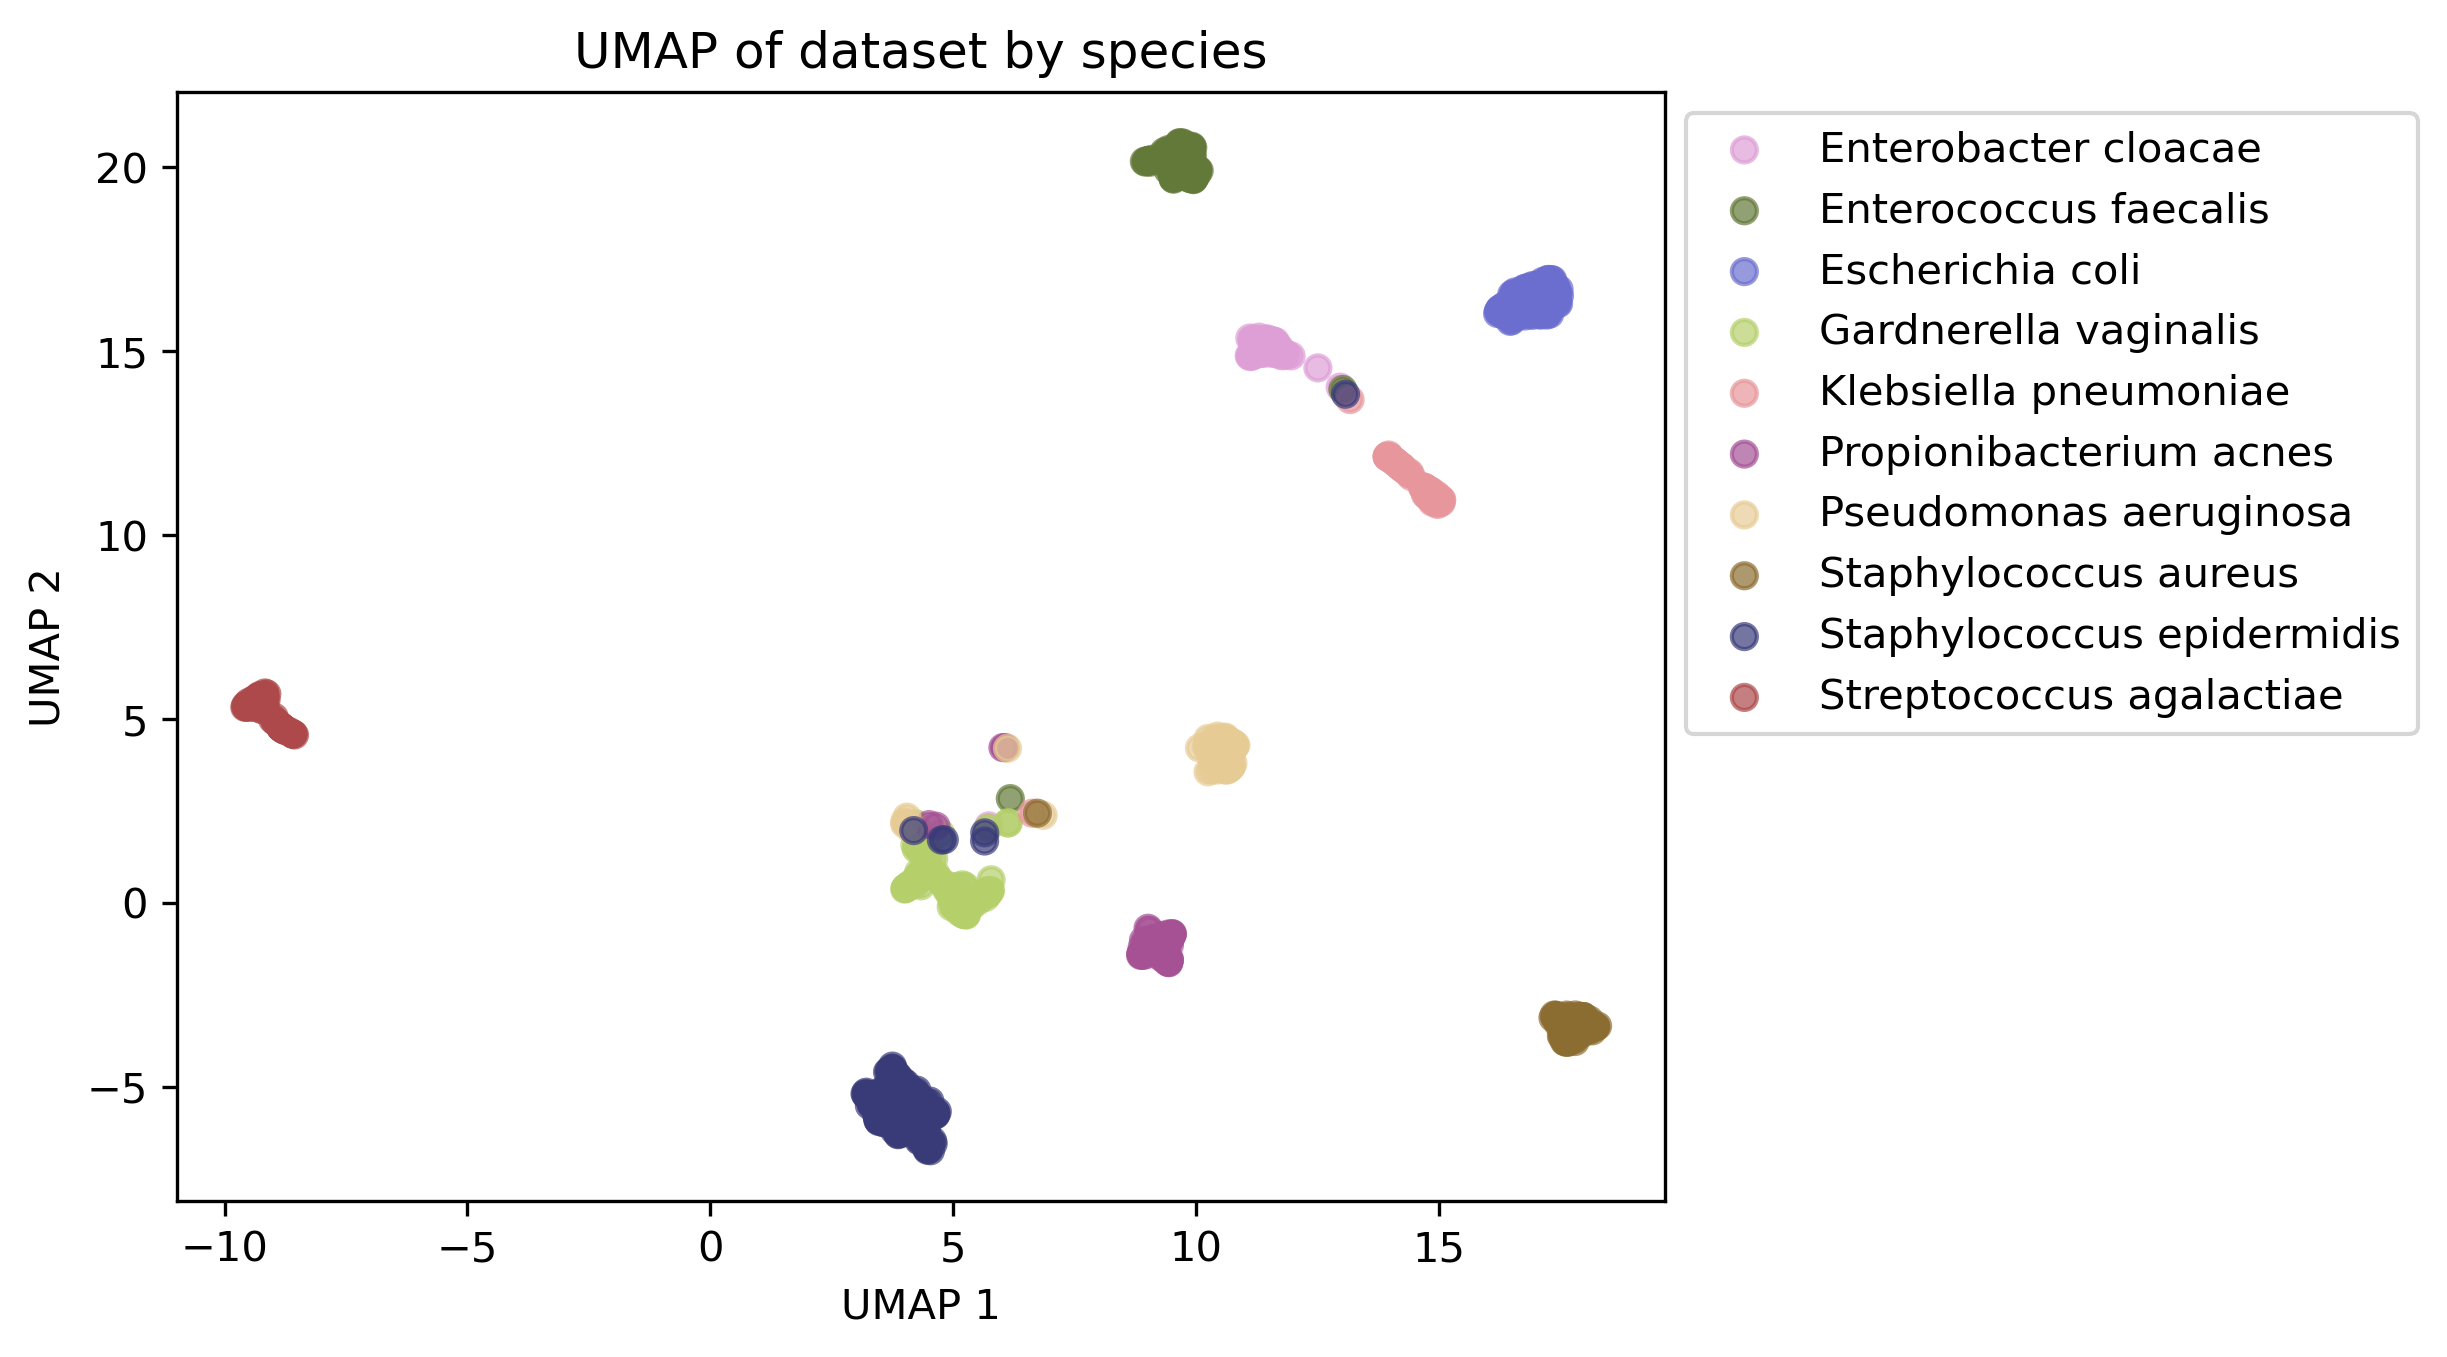
\includegraphics[width=0.9\textwidth]{img/UMAP_species_noRemaining2015.png}
	\caption{UMAP of the 2015 dataset by species.}
	\label{fig:umap_2015}
\end{figure}

\begin{figure}[h]
	\centering
	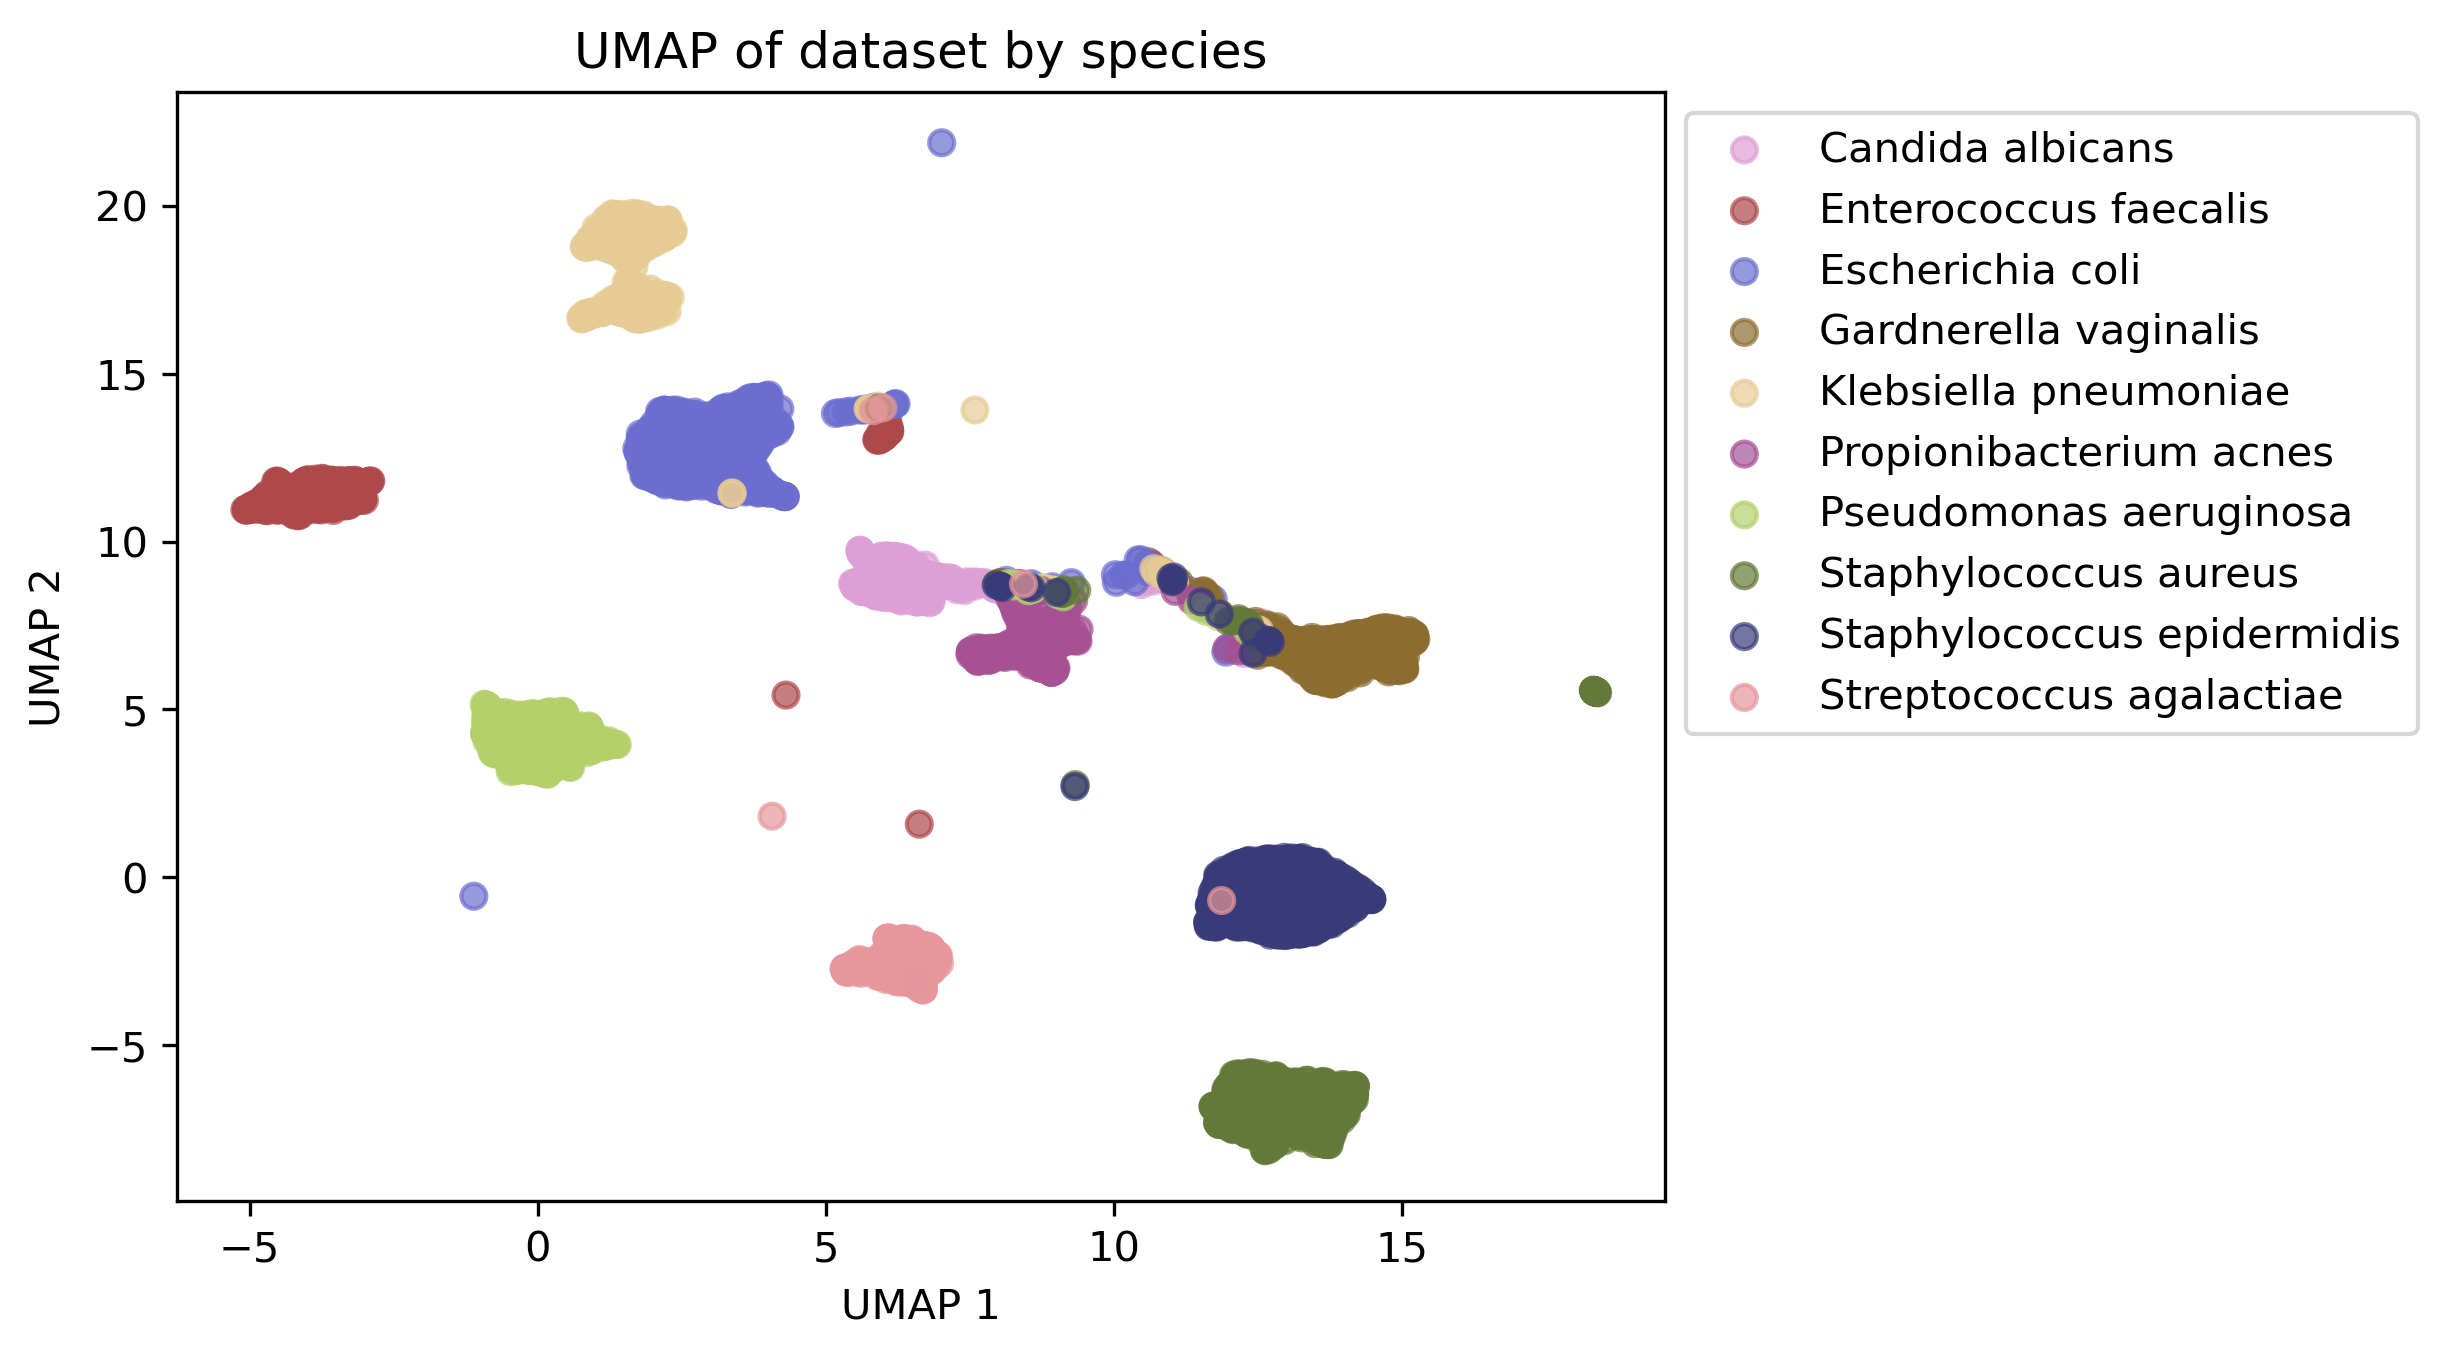
\includegraphics[width=0.9\textwidth]{img/UMAP_species_noRemaining2017.png}
	\caption{UMAP of the 2017 dataset by species.}
	\label{fig:umap_2017}
\end{figure}

\begin{figure}[h]
	\centering
	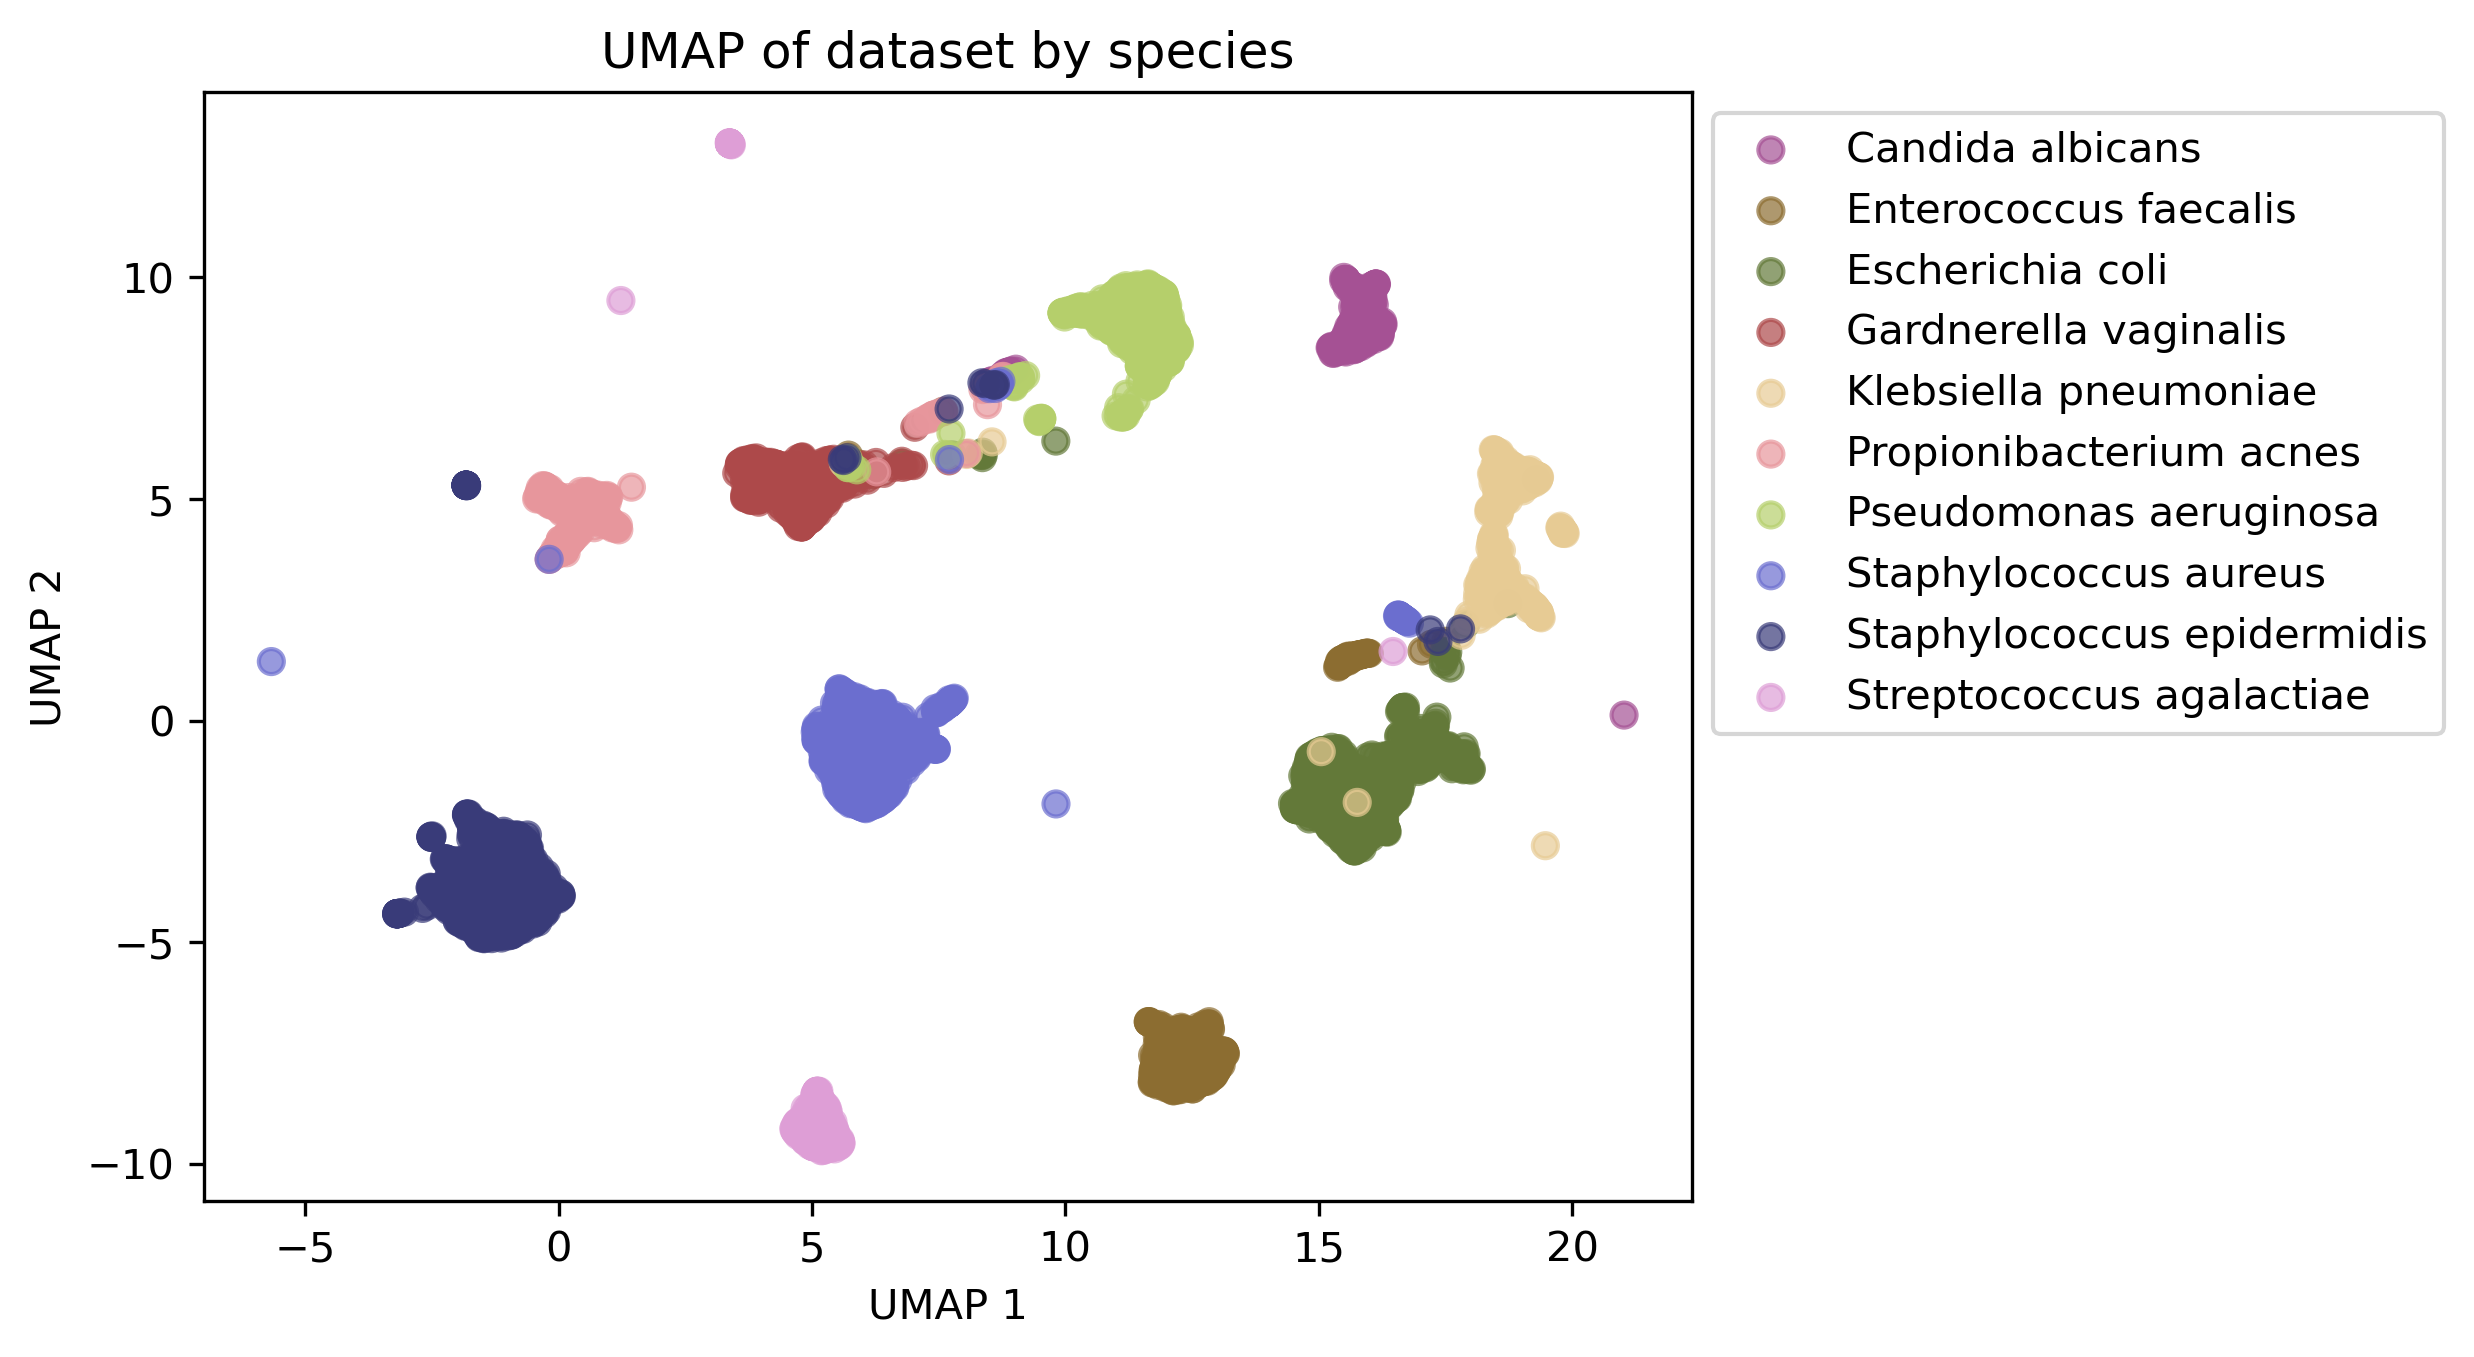
\includegraphics[width=0.9\textwidth]{img/UMAP_species_noRemaining2018.png}
	\caption{UMAP of the 2018 dataset by species.}
	\label{fig:umap_2018}
\end{figure}

\begin{figure}[h]
	\centering
	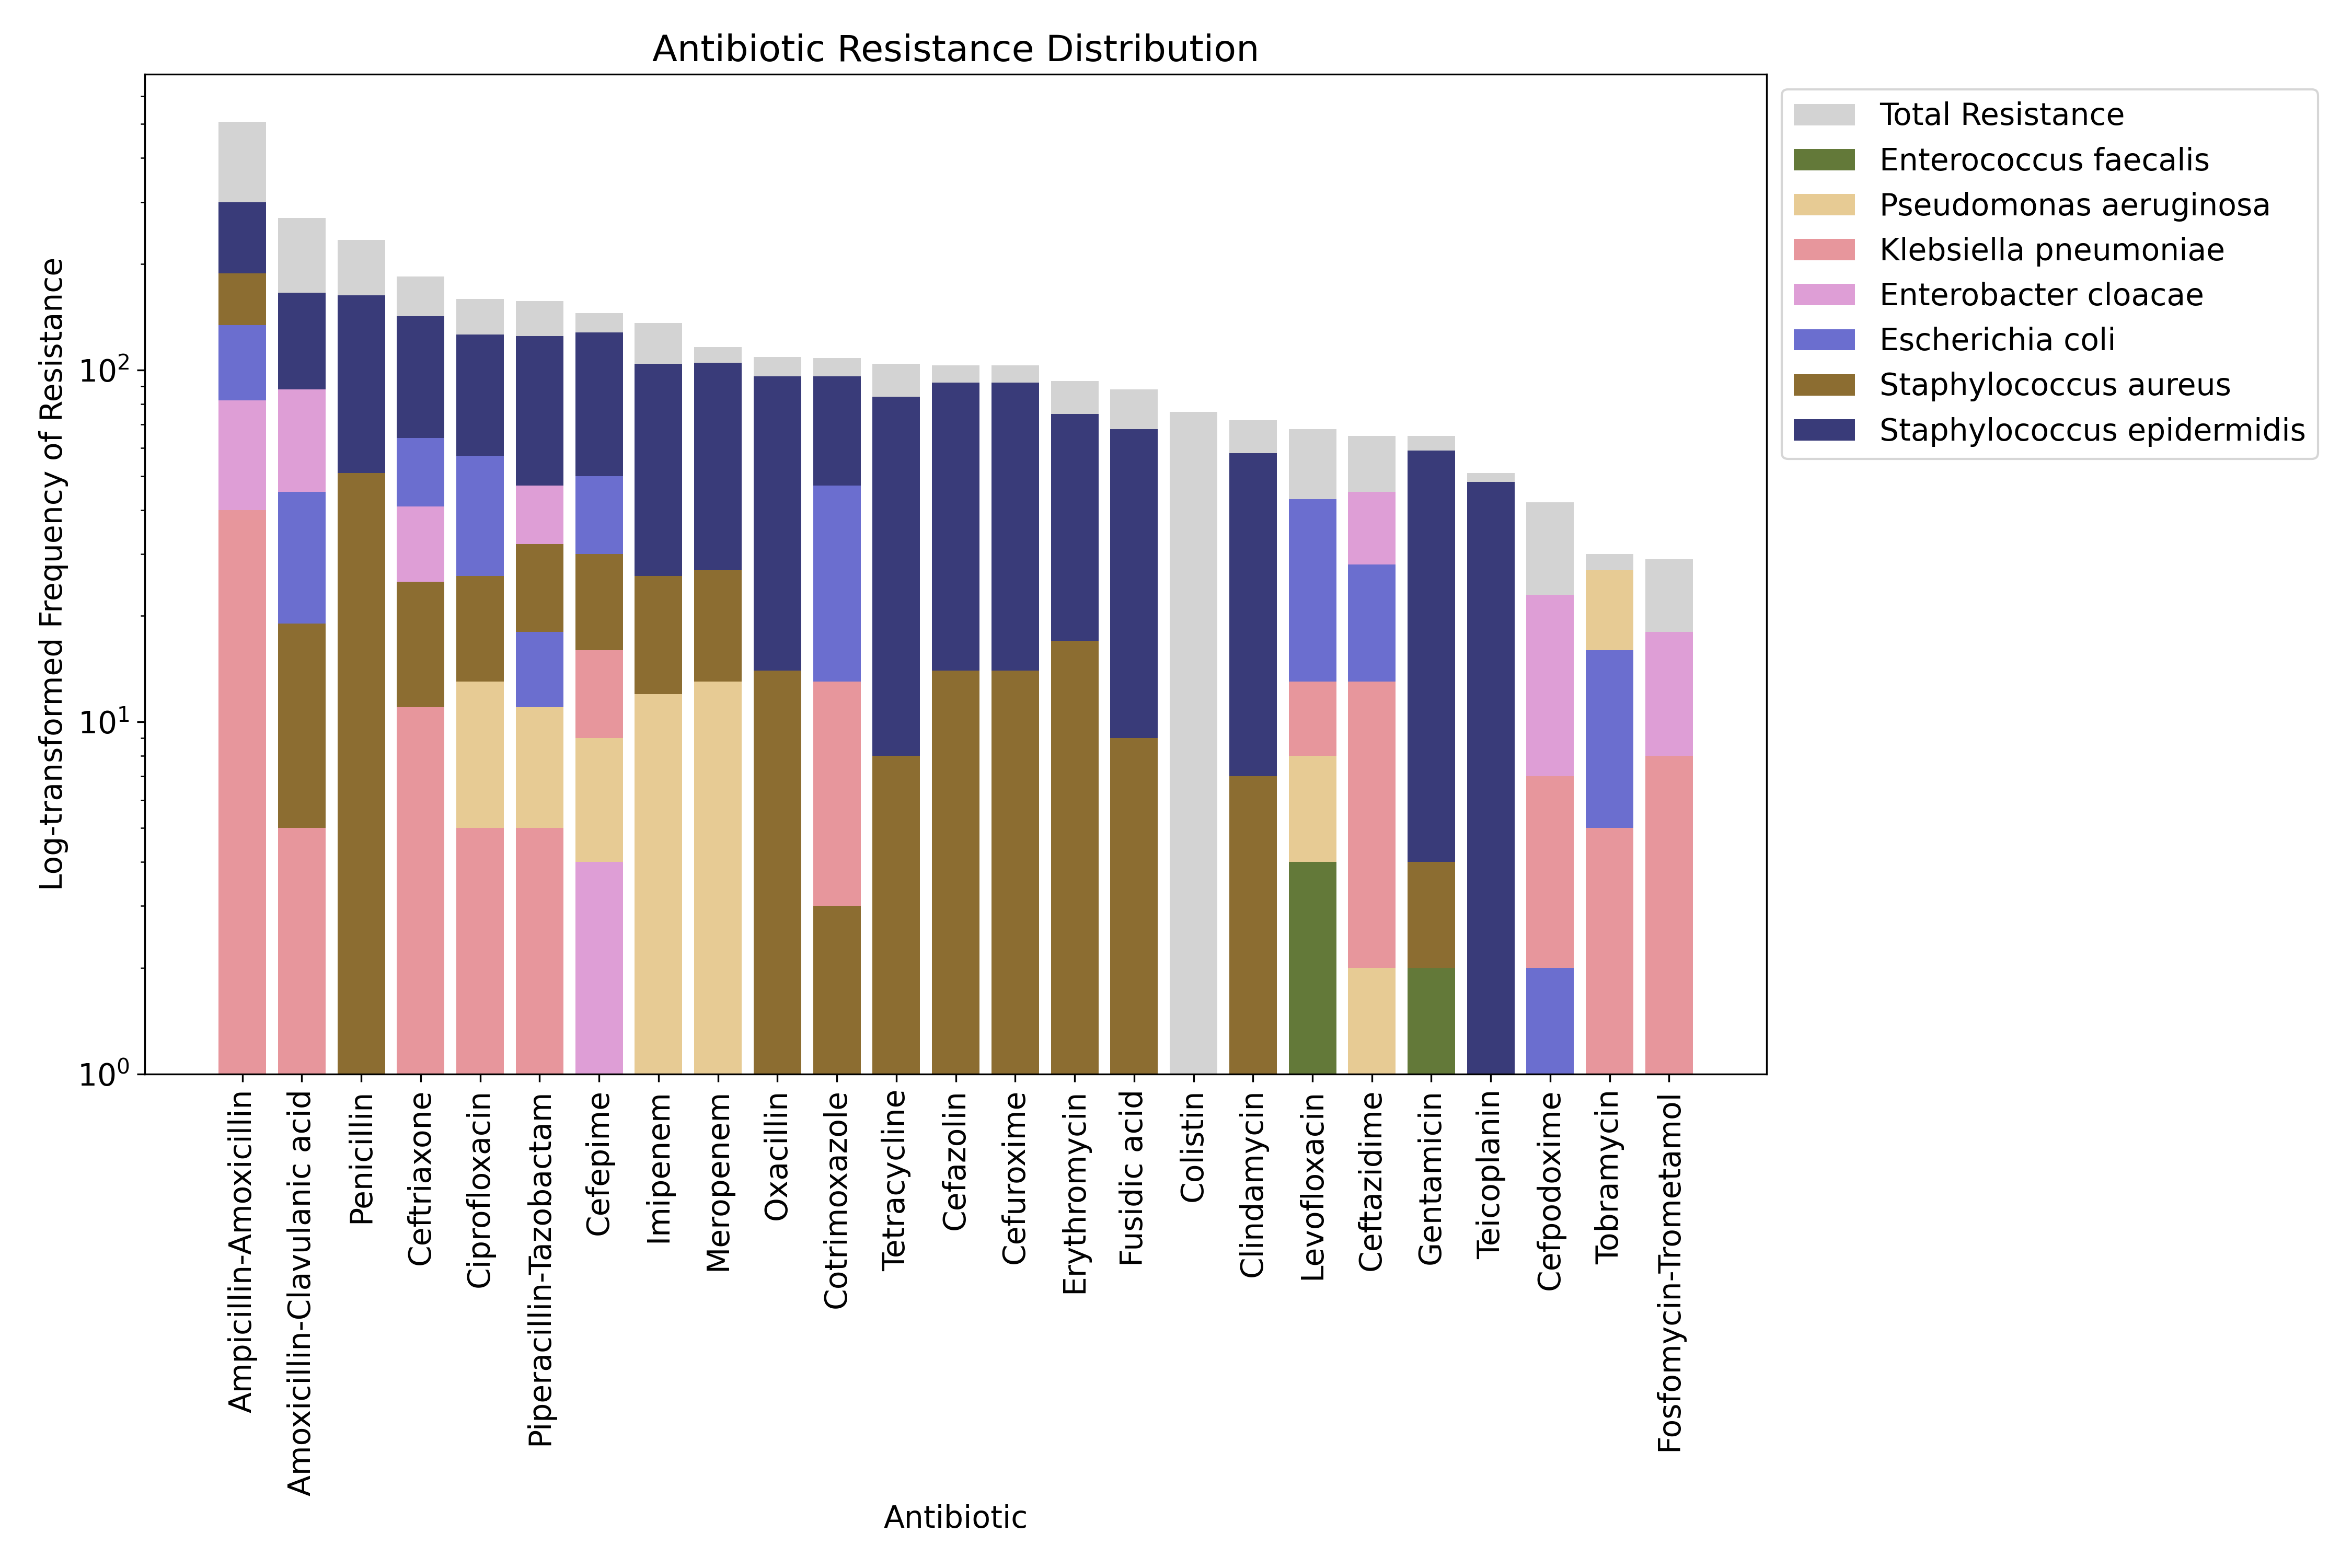
\includegraphics[width=0.9\textwidth]{img/antibiotic_resistance_distribution_filtered_2015.png}
	\caption{Antibiotic resistance distribution for 2015}
	\label{fig:resistance_distribution_2015}
\end{figure}

\begin{figure}[h]
	\centering
	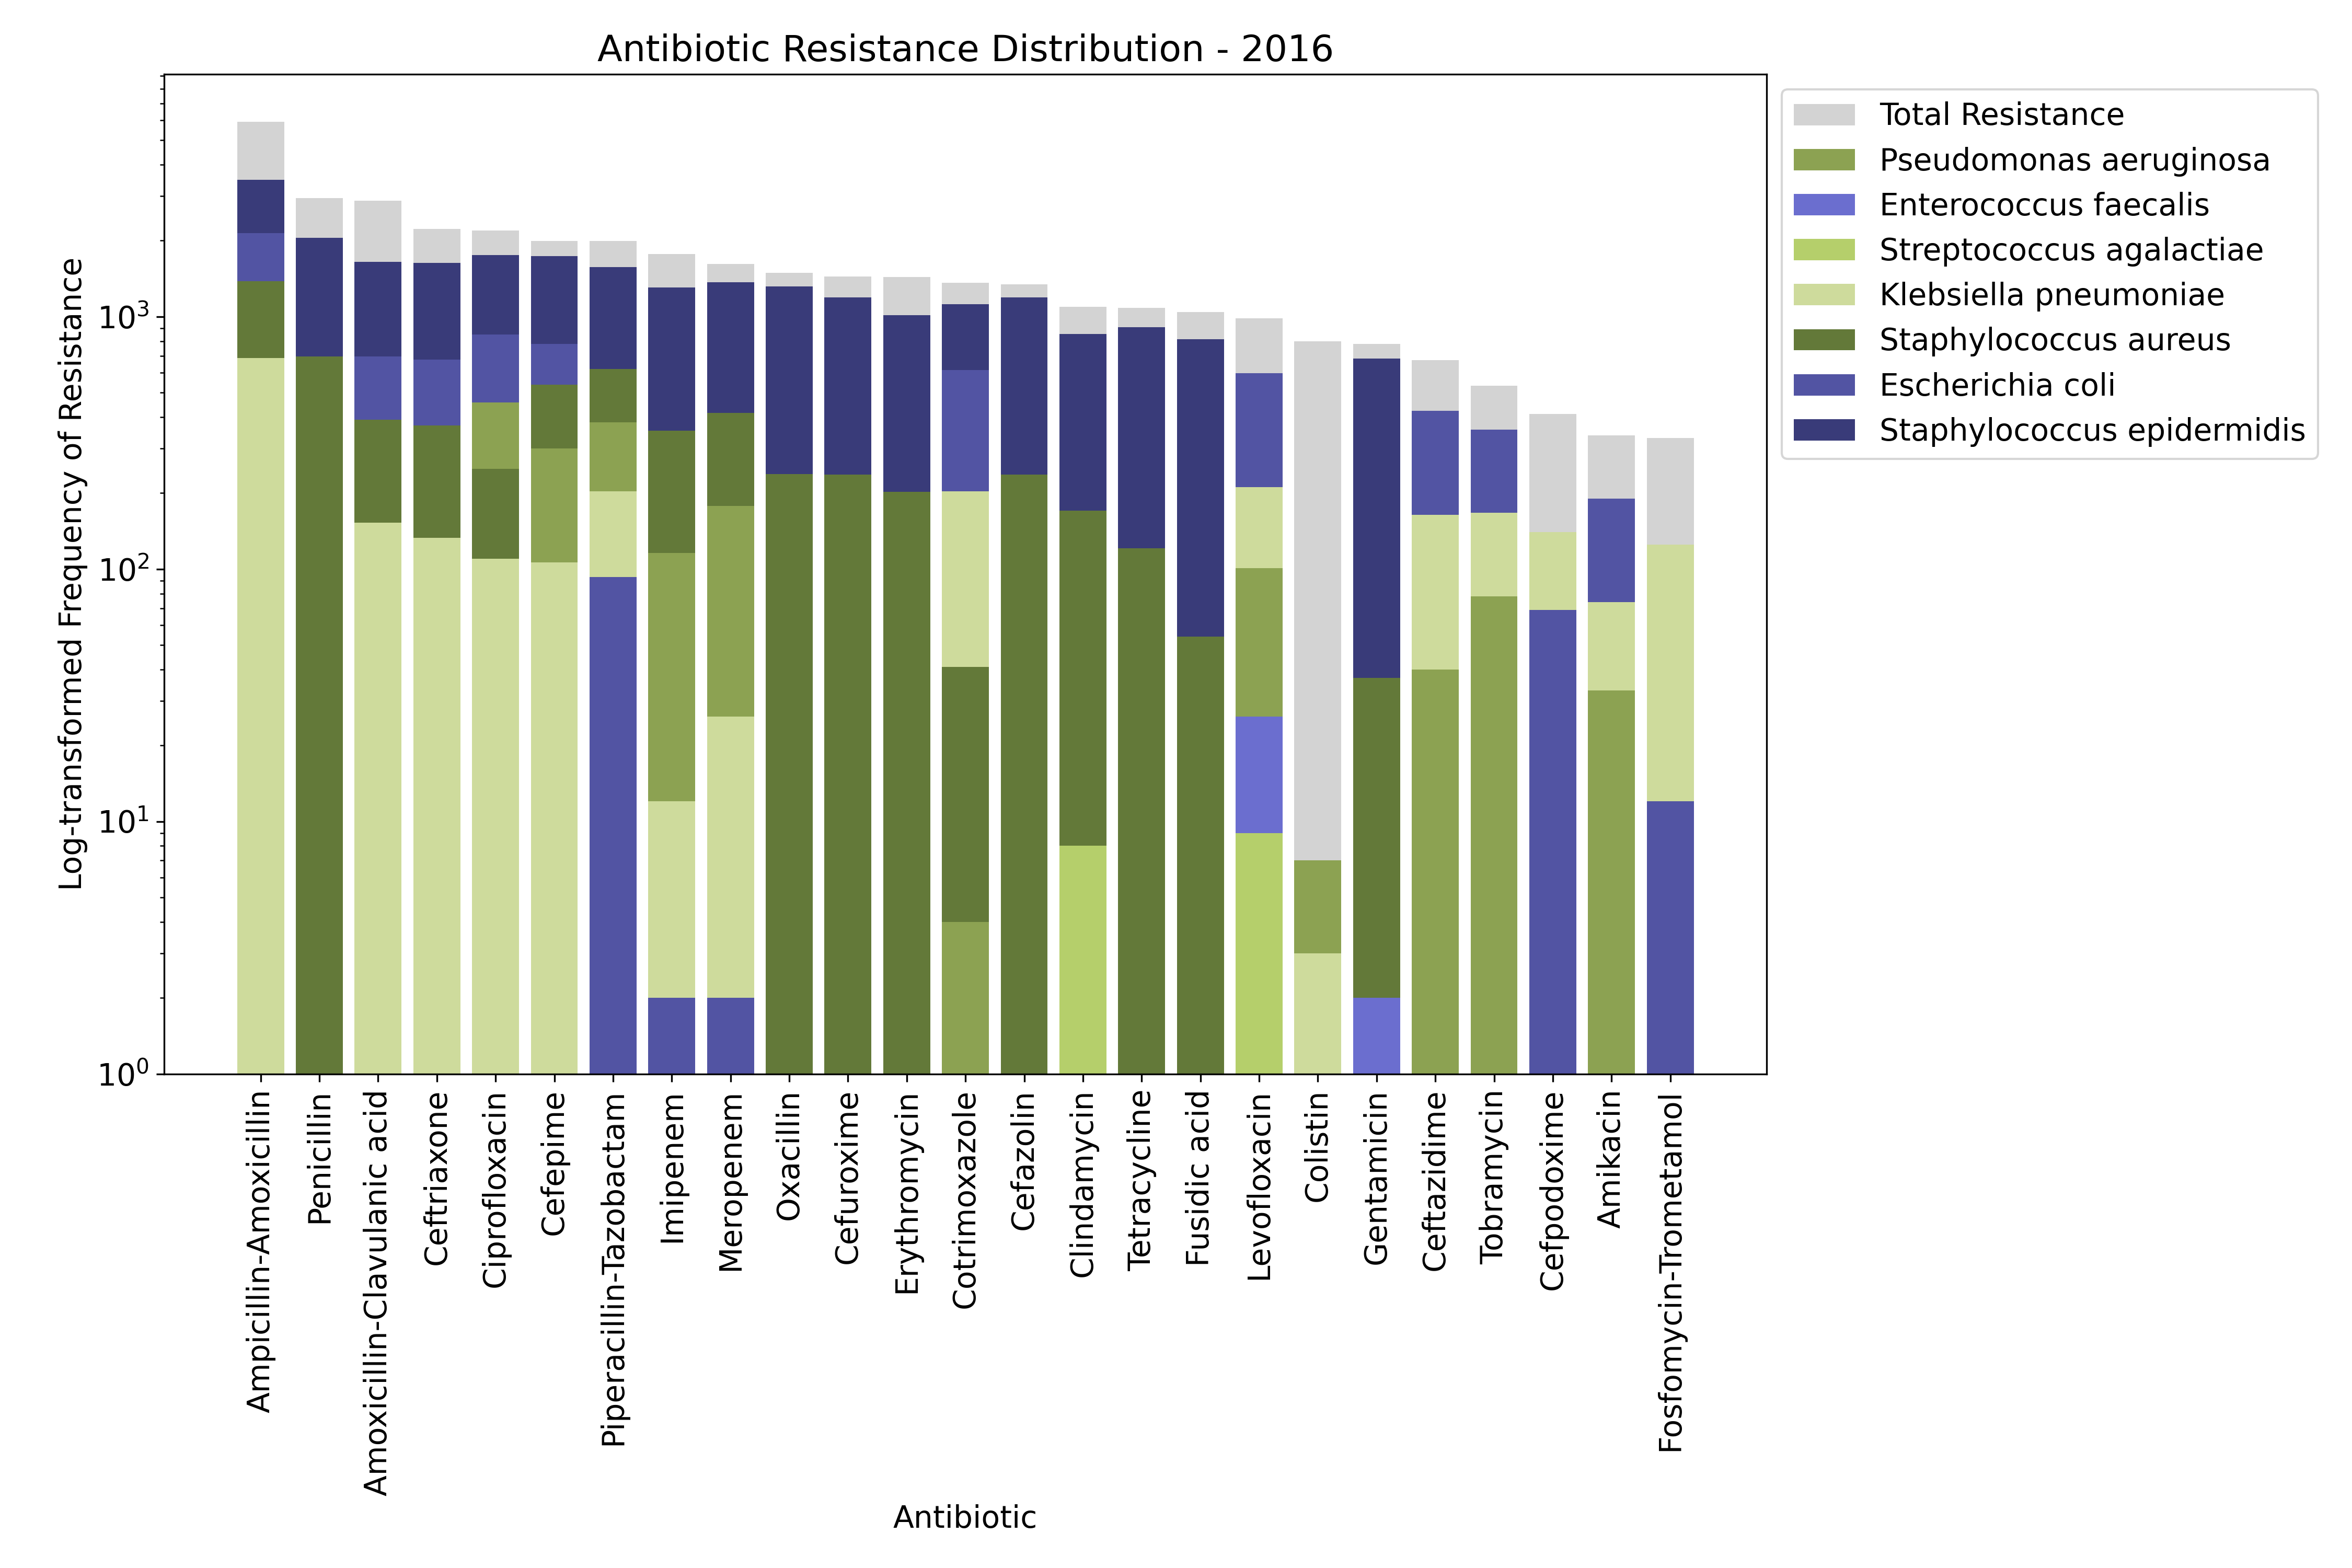
\includegraphics[width=0.9\textwidth]{img/antibiotic_resistance_distribution_filtered_2016.png}
	\caption{Antibiotic resistance distribution for 2016}
	\label{fig:resistance_distribution_2016}
\end{figure}

\begin{figure}[h]
	\centering
	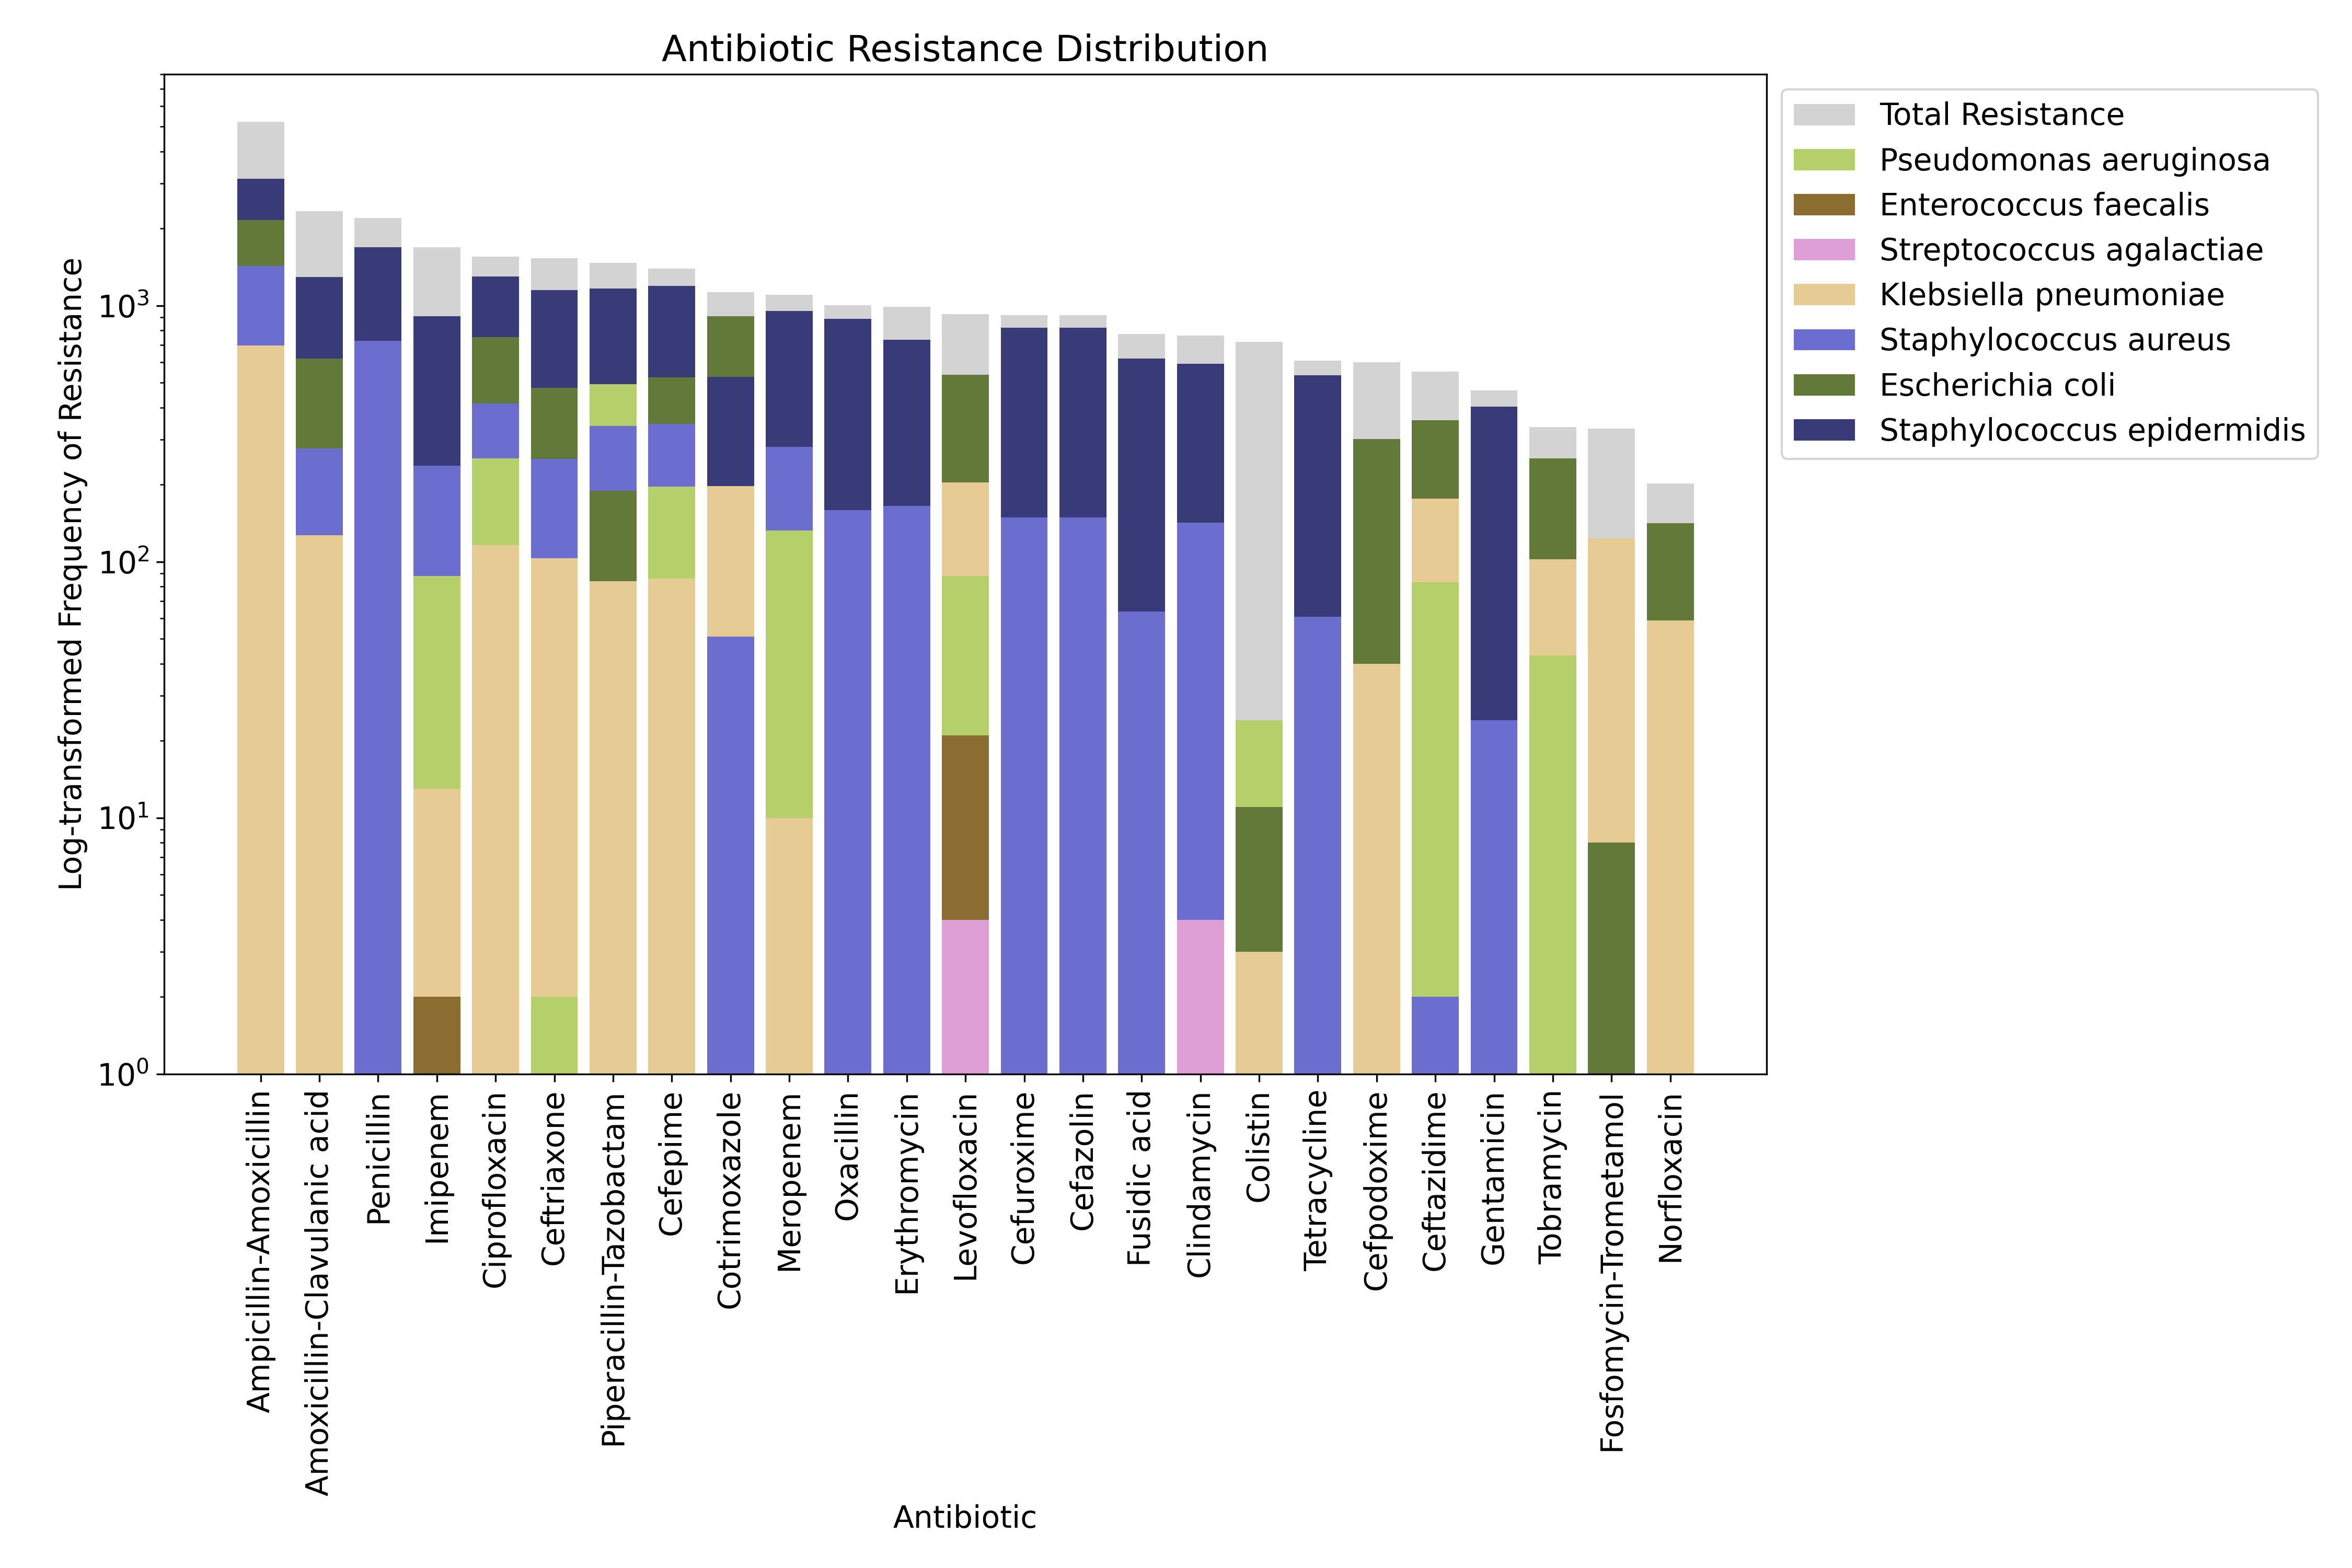
\includegraphics[width=0.9\textwidth]{img/antibiotic_resistance_distribution_filtered_2018.png}
	\caption{Antibiotic resistance distribution for 2018}
	\label{fig:resistance_distribution_2018}
\end{figure}



\end{document}